\documentclass{book}\usepackage{knitr}

% Preamble

%%%%%%%%%%%%%%%%%%%%%%
%% PACKAGES
%%%%%%%%%%%%%%%%%%%%%%
\usepackage[twoside,letterpaper,width=6in,height=8in]{geometry}
\usepackage{siunitx} % format units properly
\usepackage{wrapfig}
\usepackage[margin=10pt,font=small,labelfont=bf]{caption} % format captions
\usepackage{booktabs} % nicer tables
\usepackage{subcaption} 
\usepackage{csquotes} % block quotes
\usepackage{tikz}
\usepackage[inline, shortlabels]{enumitem} % inline enumeration
%\usepackage[version=4]{mhchem}
\usepackage{graphicx} % packages are used to modify the text and create bling.
%\includegraphics{{Home/CAMPUS/mwl04747/github/Environmnental-Sciences-in-East-Asia/images/}}
\usepackage{textcomp}
\usepackage{gensymb}
\usepackage[T1]{fontenc}
\usepackage{natbib}
%\usepackage{wasysym} %\smiley{}
% \usepackage{siunitx}
\usepackage{glossaries}
% \usepackage[automake]{glossaries} % automake option unknown.
\usepackage{amsmath}%
\usepackage{amsfonts}%
\usepackage{amssymb}%
\usepackage{soul}
\usepackage{comment}


%\usepackage[super,square,comma]{natbib}
%\usepackage{float}
%\usepackage{appendix}
%\usepackage{chngcntr}
%\usepackage{etoolbox}
%\usepackage[usenames]{xcolor}% for commenting in color!

\RequirePackage{hyperref} % For hyperlinked cross-references
\hypersetup{
    colorlinks,
    citecolor=blue,
    filecolor=blue,
    linkcolor=blue,
    urlcolor=blue
}

% Editorial Environments

\newcommand{\red}[1]{\textcolor{red}{[MLH: #1]}}
\newcommand{\blue}[1]{\textcolor{blue}{[MLH: #1]}}

%-----------------------------------------------------
\newtheorem{theorem}{Theorem}
\newtheorem{acknowledgement}[theorem]{Acknowledgement}
\newtheorem{definition}[theorem]{Definition}
\newtheorem{example}[theorem]{Example}
\newtheorem{exercise}[theorem]{Exercise}

\newtheorem{problem}[theorem]{Problem}
\newtheorem{remark}[theorem]{Remark}
\newtheorem{solution}[theorem]{Solution}
\newtheorem{summary}[theorem]{Summary}
\newenvironment{proof}[1][Proof]{\textbf{#1.} }{\ \rule{0.5em}{0.5em}}
%----------------------------------------------------------

\AtBeginEnvironment{subappendices}{%
\chapter*{Appendix}
\addcontentsline{toc}{chapter}{Appendices}
%\counterwithin{figure}{section}
%\counterwithin{table}{section}
}

\makeatletter
\newcommand{\chapterauthor}[1]{%
  {\parindent0pt\vspace*{-25pt}%
  \linespread{1.1}\large\scshape#1%
  \par\nobreak\vspace*{35pt}}
  \@afterheading%
}
\makeatother

\renewcommand{\glstextformat}[1]{\textbf{\color{blue}\em #1}}

\newcommand{\R}{\mathbb{R}}
\newcommand{\carbondioxide}{CO$_2$~}
\newcommand{\kms}{km$^2$}

\newcommand{\Mypm}{\mathbin{\tikz [x=1.4ex,y=1.4ex,line width=.1ex] \draw (0.0,0) -- (1.0,0) (0.5,0.08) -- (0.5,0.92) (0.0,0.5) -- (1.0,0.5);}}%



\title{Environmental Issues in East Asia}
\author{EA30e Spring 2021}
\date{\today}
\IfFileExists{upquote.sty}{\usepackage{upquote}}{}
\begin{document}
\makeglossaries
\maketitle


\frontmatter
\tableofcontents


\chapter*{Preface}

\section{Guiding Principles}

Environmental issues in East Asia are not unique or particularly more prevasive than other parts of the world. However, the issues are born from particular histories that may contrast with other parts of the world and other parts of the world may be able to learn from. 

In this project, the students in EA030e (Spring 2021) have written a textbook that highlights examples of environmental processes. Each student contributed to one theme, composed of two examples that highlight environmental issues of East Asia. 

\subsection{Context and Positionality}

As students in a college course located in Southern California, we approach the project with...


Our goal is not to call out environmental issues in East Asia, but to point to linkages of how a range of globalized economy contribute to these environmental problems. 

In the end, it would be useful for us to acknowledge we have some capacity to address these how these global linkages could be modified to reduce these environmental issues.

We are not experts, but learning... if there are errors please let us know... We recommend that suggestions be submitted via a github pull request.

\subsection{Goals}

Processes across horizontal boundaries define many environmental patterns that frame human interactions with the environment. How do humans impact processes that cross these boundaries and how do humans influence these ecosystem interface?

\subsection{Rationale}

We hope to learn more about the how environmental issues are expressed in different parts of the world and to what extent can we learn from this work. 

\subsection{Activity}

Each group will be composed of two students, that will become experts and teach their classmates on the topic. 

\section{East Asia and the World}







\section{Acknowledgments}

Everyone in the world!




\chapter{\LaTeX Guide}\label{ch:guide}

\section*{Why Learn \LaTeX?}

\subsection*{Creating Professional Typesetting}

In the past, I used \LaTeX to make publication quality text. In fact, many prefer writing in \LaTeX because they can focus on the text and avoid worrying about formatting. However, it is NOT WYSIWYG (``what you see is what you get'') word processor. In reality, the processing or compiling is a separate step. 

Nevertheless, the quality of the output and ability to integrate with R (or Python) allows us to have an exceptional tool to make reproducible documents with highly professional looking typesetting.

\subsection*{How to Learn \LaTeX?}

There are several ways to learn \LaTeX. I suggest you find a decent tutorial to get the basics. For example, here are some suggestions:

\begin{itemize}
  \item \href{https://www.overleaf.com/learn/latex/Learn_LaTeX_in_30_minutes}{Learning \LaTeX in 30 minutes}
\end{itemize}

If you are like me and can't remember commands very well, then here's a \href{https://wch.github.io/latexsheet/latexsheet-0.png}{cheet sheet} that might be helpful. 

\subsubsection{R Chunks}

To create effective graphics, each chapter will have a rchunk that creates a graphic for the chapter. To review and learn R, here are some resources: 

\begin{itemize}
  \item \href{www.tbd.com}{Marc's Video Description}
  \item \href{https://rmd4sci.njtierney.com/}{RMarkdown for Scientists (super helpful!)}
  \item \href{https://rmarkdown.rstudio.com/lesson-1.html}{R Studio Tutorial}
  \item \href{https://rstudio.com/wp-content/uploads/2016/03/rmarkdown-cheatsheet-2.0.pdf?_ga=2.107420162.161662097.1613074083-214354297.1613074083}{R Studio's Cheatsheet}
  \item \href{https://bookdown.org/yihui/rmarkdown-cookbook}{R Markdown Cookbook -- Robust Source}
\end{itemize}


\subsection*{Noting Your Contribution}

Because this is an ongoing project, you should record your contribution to each chapter -- but also let go of these contributions at some point; Others might revise and their authorship might take some precedence, so you should both invest in the product but also be willing to detach from the final outcome as others contribute. This will feel uncomfortable at times, but please note from the beginning this is a social process and as such subject to negotiation. Please be generous to the authors that laid the foundation and be respectful of those that follow. 

\section{Setting Up Book Project--Type Setting w/ \LaTeX}\label{sec:settingup}

\subsection{Latex Book Class}

Currently, the text is written using the standard book class. %However, in 2019, I (Los Huertos) will convert the format to a Tufte book class. 

\subsection*{Structuring the Text with Nested Hierarchies}

Contributors divide their contributions into sections and subsections. This format allows a consistent approach to structuring the text and forcing themes to be organized in blocks that can be used to organize the overall text. We use section, subsection, and subsubsection to break up the topic into bite sizes. 

To accomplish this, contributors use the \verb"\section{Section}" command for major sections, and the \verb"\subsection{Subsection}" command for subsections, and a similar approach for subsubsections. 

NOTE: for each nested level, it MUST be followed by the lowest level in the section before a paragraph is started -- in contrast to what is shown above!

NOTE: We may dispense with subsubsections in the future to provide a less blocky structure, but for now they remain useful. 

\subsection*{Font Changes}

We can use various methods to alter the typeset: \emph{Emphasize}, \textbf{Bold}, \textit{Italics}, and \textsl{Slanted}. We can also typeset \textrm{Roman}, \textsf{Sans Serif}, \textsc{Small Caps}, and \texttt{Typewriter} texts.  Look online to see the commands to accomplish these changes. 

You can also apply the special, mathematics only commands $\mathbb{BLACKBOARD}$, $\mathbb{BOLD}$, $\mathcal{CALLIGRAPHIC}$, and $\mathfrak{fraktur}$. Note that blackboard bold and calligraphic are correct only when applied to uppercase letters A through Z.

You can apply the size tags -- Format menu, Font size submenu -- {\tiny tiny}, {\scriptsize scriptsize}, {\footnotesize footnotesize}, {\small small}, {\normalsize normalsize}, {\large large}, {\Large Large}, {\LARGE LARGE}, {\huge huge} and {\Huge Huge}.

You can use the \verb"\begin{quote} etc. \end{quote}" environment for typesetting short quotations. Select the text then click on Insert, Quotations, Short Quotations:

\begin{quote}
The buck stops here. \emph{Harry Truman}

Ask not what your country can do for you; ask what you can do for your
country. \emph{John F Kennedy}

I am not a crook. \emph{Richard Nixon}

I did not have sexual relations with that woman, Miss Lewinsky. \emph{Bill Clinton}
\end{quote}

The Quotation environment is used for quotations of more than one paragraph. Following is the beginning of description of \LaTeX from \emph{Wikipedia}:

\begin{quotation}
LaTeX (/ˈlɑːtɛx/ LAH-tekh or /ˈleɪtɛx/ LAY-tekh, often stylized as \LaTeX) is a software system for document preparation. When writing, the writer uses plain text as opposed to the formatted text found in ``What You See Is What You Get'' word processors like Microsoft Word, LibreOffice Writer and Apple Pages. The writer uses markup tagging conventions to define the general structure of a document (such as article, book, and letter), to stylise text throughout a document (such as bold and italics), and to add citations and cross-references. A \TeX distribution such as \TeX Live or MiK\TeX is used to produce an output file (such as PDF or DVI) suitable for printing or digital distribution.

\LaTeX is widely used in academia for the communication and publication of scientific documents in many fields, including mathematics, statistics, computer science, engineering, physics, economics, linguistics, quantitative psychology, philosophy, and political science. It also has a prominent role in the preparation and publication of books and articles that contain complex multilingual materials, such as Sanskrit and Greek. \LaTeX uses the \TeX typesetting program for formatting its output, and is itself written in the TeX macro language.''
\end{quotation}

Use the Verbatim environment if you want \LaTeX\ to preserve spacing, perhaps when
including a fragment from a program such as:
\begin{verbatim}
#read csv data  // read data into R
my.dataframe <- read.csv(file.choose())   // read data from a popup window.

str(my.dataframe) // display data structure

\end{verbatim}
(After selecting the text click on Insert, Code Environments, Code.)


\subsection*{Mathematics and Specialized Characters}\label{sub:mathchar}

\subsubsection*{Warning: Special Characters}

When you use percent and ampersand symbols, hash tags, and other non-standard ASCII characters, \LaTeX will be very uncooperative. \LaTeX~doesn't like a range of characters or they reserved for special behavior. So, do yourself a favor and make sure you understand that these are used for special typesetting functions. To use them you have to ``escape'' and use commands to get them to do what you might usually expect!  

The following symbols \$, \%, \#, \&, \`e, \~n, `` and '' do not reflect the key stroke you might expect. 

For example, the \& is used for tabs in a table environment. \% is used to make comments, thus stuff behind a \% is ignored. There are lots of others, but these come up the most. If you want to show use the ampersand or one of these characters, put a backslash in front of the dollar sybmol, e.g. \textbackslash\$. See Table \ref{tab:tableofsymbols}.

If you want to a superscript (raised to 3nd power), we can create text in math mode, with \$ to start and end the text in math mode, e.g. m$^3$ is written in \LaTeX as m\$\^{}3\$. A subscript uses an underscore, x\$\_1\$ creates x$_1$. If you need more than one character as a subscript or superscript then enclose the content in curly brakets, e.g. x$^{2c}$ (x\$\^{}\{2c\}\$) and t$_{step}$ (t\$\_\{step\}\$).

\begin{table}[h]
\caption{Table of Symbols in \LaTeX}
\label{tab:tableofsymbols}
\begin{tabular}{|ll|ll|} \hline
Symbol  & \LaTeX code & Symbol & \LaTeX code \\ \hline\hline
\&  & \textbackslash\&  & 
\$  & \textbackslash\$ \\
``  & \`{}\`{} & 
''  & \'{}\'{} \\
mg~L$^{-1}$ & mg$\sim${}L\$\^{}\{-1\}\$ & 
    & \\ 
\hline
\end{tabular}

\end{table}

\subsection{Creating equations}

One of the most powerful parts of \LaTeX is how it can be used to write complex equations, with all those symbols and Greek letters! This can be done inline $y = mx + b + \epsilon$ for fairly simple equations, or set apart for more complex equations:

\begin{equation}
\int_0^\infty e^{-x^2} dx=\frac{\sqrt{\pi}}{2}
\end{equation}

\subsubsection{Theorems, etc}
\begin{theorem}
(The Currant minimax principle.) Let $T$ be completely continuous selfadjoint operator
in a Hilbert space $H$. Let $n$ be an arbitrary integer and let $u_1,\ldots,u_{n-1}$ be
an arbitrary system of $n-1$ linearly independent elements of $H$. Denote
\begin{equation}
\max_{\substack{v\in H, v\neq
0\\(v,u_1)=0,\ldots,(v,u_n)=0}}\frac{(Tv,v)}{(v,v)}=m(u_1,\ldots, u_{n-1})
\label{eqn10}
\end{equation}
Then the $n$-th eigenvalue of $T$ is equal to the minimum of these maxima, when
minimizing over all linearly independent systems $u_1,\ldots u_{n-1}$ in $H$,
\begin{equation}
\mu_n = \min_{\substack{u_1,\ldots, u_{n-1}\in H}} m(u_1,\ldots, u_{n-1}) \label{eqn20}
\end{equation}
\end{theorem}
The above equations are automatically numbered as equation (\ref{eqn10}) and
(\ref{eqn20}).


\subsection*{Lists Environments: Making bulletted, numbered, description lists}

We use special commands to create an itemized list.

You can create numbered, bulleted, and description lists
(Use the Itemization or Enumeration buttons, or click on the Insert menu
then chose an item from the Enumeration submenu):

\begin{enumerate}
\item List item 1

\item List item 2

\begin{enumerate}
\item A list item under a list item.

\item Just another list item under a list item.

\begin{enumerate}
\item Third level list item under a list item.

\begin{enumerate}
\item Fourth and final level of list items allowed.
\end{enumerate}
\end{enumerate}
\end{enumerate}
\end{enumerate}

\begin{itemize}
\item Bullet item 1

\item Bullet item 2

\begin{itemize}
\item Second level bullet item.

\begin{itemize}
\item Third level bullet item.

\begin{itemize}
\item Fourth (and final) level bullet item.
\end{itemize}
\end{itemize}
\end{itemize}
\end{itemize}

\begin{description}
\item[Description List] Each description list item has a term followed by the
description of that term.

\item[Bunyip] Mythical beast of Australian Aboriginal legends.
\end{description}

\subsection*{Theorem-Like Environments}

The following theorem-like environments (in alphabetical order) are available
in this style.

%\begin{acknowledgement}
%This is an acknowledgement
%\end{acknowledgement}

\begin{example}
This is an example
\end{example}

\begin{exercise}
This is an exercise
\end{exercise}


%\begin{proof}
%This is the proof of the lemma.
%\end{proof}

%\begin{notation}
%This is notation
%\end{notation}

%\begin{problem}
%This is a problem
%\end{problem}

%\begin{proposition}
%This is a proposition
%\end{proposition}

%\begin{remark}
%This is a remark
%\end{remark}

%\begin{summary}
%This is a summary
%\end{summary}

\begin{theorem}
This is a theorem
\end{theorem}

%\begin{proof}
%[Proof of the Main Theorem]This is the proof.
%\end{proof}

\subsubsection*{``Child'' Rnw Contributions to create a Textbook}

To create the texbook, we will each contribut chapters, which are referred to in knitr speak as a `child'. For each `child' or chapter, will be a sepreate Rnw fild, but without the need for the preamble, such as the \verb"\begin{document}" and \verb"\end{document}", which is pretty handy. Then each chapter has the exact same formatting as defined in the root document, which you have to select in the project options. 

\subsection*{Peer Review Commenting}

You can put your comments in square brackets and in color for things that need help. \textcolor{red}{[This section is confusing, I am not sure what commenting means.]} I have created a short cut command to do this with \verb"\red{}". 

\subsection*{Adding Figures, etc}

\subsubsection*{Using Rnw Files}

To generate R figures, we use R chunks in and Rnw file, where the text is integreated. When we compile into a PDF, the program converts the files into TeX files and then combineds them into a single pdf. 

For each chapter, we create a ``child'' document and Marc will help you create that text when you begin. 

\subsubsection*{Creating a floating figure}

This is my floating figure (Figure \ref{fig:plot}).

\begin{figure}

\caption{My plot's caption is here!}
\label{fig:plot}
\end{figure}

\subsubsection*{Using R to Create Effective Figures}

R Markdown can be a very powerful tool to integrate R code, figures and text. Making high quality figures that are both clear and aestically pleasing will be something that we need to think about it. 

\begin{itemize}
  \item Axis Labels -- Labelled with clarity 
  \item Axis Text -- Size, Orientation 
  \item Captions (usually better than titles)
  \item References connecting labels to references
  \item ADA accessible (e.g. color impairment mitigation)
\end{itemize}

For example, here's an example of a pretty good figure, and you can find the code in the 01-guide.Rnw file.





In the case of Figure~\ref{fig:co2-graphic}, we can a create a figure that has all of the characteristics listed above, except perhaps ADA. Creating a "alt text" for the figure is something we might want to consider -- For now a decent caption about what the reader is seing is super helpful. 

\begin{figure}
\begin{knitrout}
\definecolor{shadecolor}{rgb}{0.969, 0.969, 0.969}\color{fgcolor}
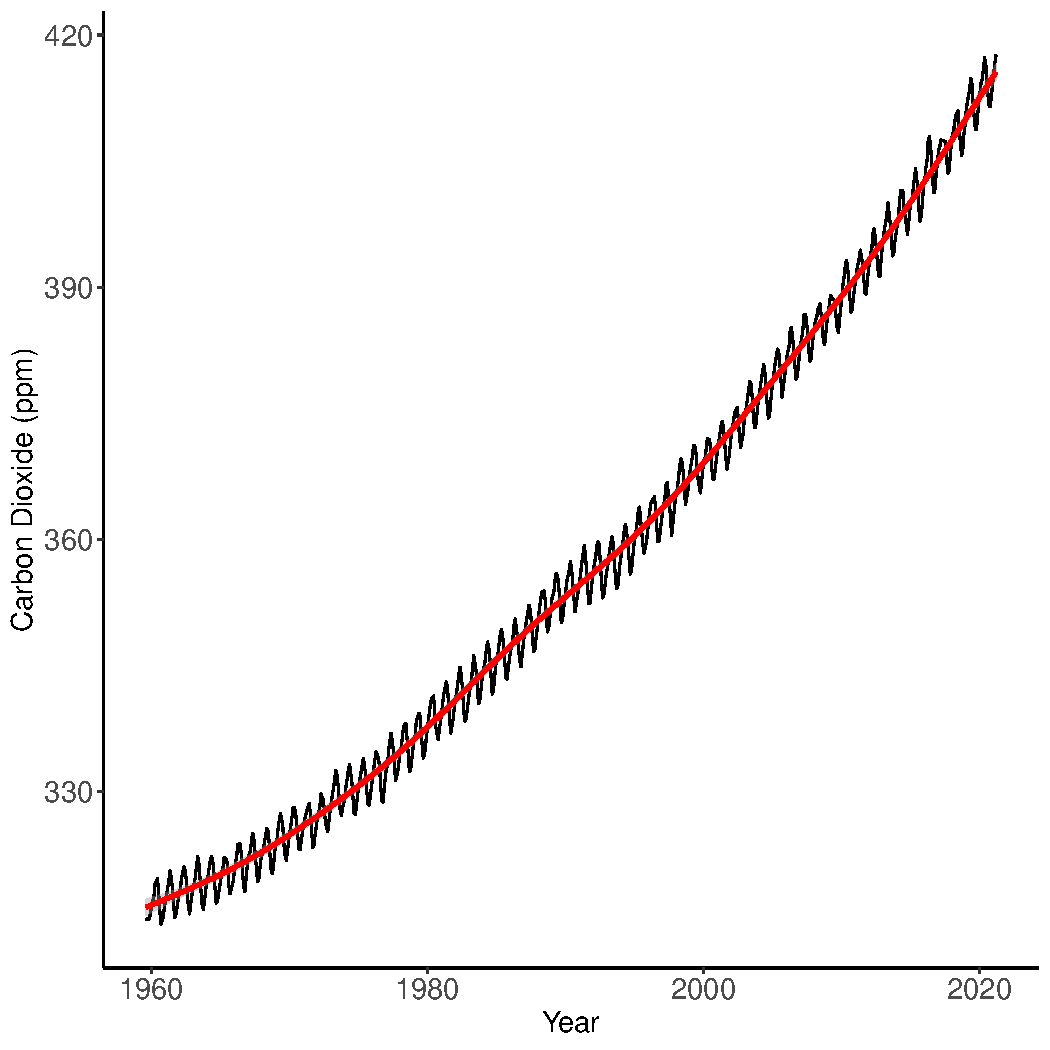
\includegraphics[width=\maxwidth]{figure/maunaloa-1} 

\end{knitrout}
\caption{Carbon Dioxide Concentrations (Mauna Loa, HI). Data demonstrate the CO$2$ concentrations are increases, but that a seasonal impact is embedded in the long-term trend. Source: Scripps/NOAA.}
\label{fig:co2-graphic}
\end{figure}

\subsection*{Using Boxes}

\fbox{
\begin{minipage}[c]{.9\textwidth}
\subsection{minibox X}

Some text
\end{minipage}
}

\section*{Cross-References, Citations, and Glossaries}

\subsection*{Cross-References}

We can cross-reference sections (e.g. Section~\ref{ch:critical-zone}  or figures (Figure~\ref{fig:maunaloa}) using several methods. I suggest you look at the this Rmd file to see how I did it in these examples.

You can also create links to URLs or hyperlinks, e.g. \url{http://texblog.org}. However, if these addresses change, then the link will break, so I suggest you only link to internal references.

\subsection*{Bibliography generation}

There will be two steps to cite our sources. First, we need to add the reference to a database, or bib file. This is titled 'References.bib' and is located in the main folder in our respository. When you add information to the bib file, be sure to paste in the reference using a bibTeX format. 

Second, we'll need to place in-line citations, using \verb"\citep{knitr}", which produces \citep{knitr}, by using a key, which is knitr in this case. 

For example, you might write, ``This document was produced in RStudio using the knitr package (\citep{knitr}). Also try \verb"\citet{LosHuertos2017OverviewR}" to create use the author name as the subject: \citet{LosHuertos2017OverviewR} wrote an guide to help students learn R. 

Note: You will see these citations automatically put in alphabetic order in the Bibliography at the end of the PDF. 

%Currently, we are using the ecology.bst, but it has trouble with misc type of references, so I will changing this in 2019. 

\subsection*{Creating glossary words}
 
Not sure why, I haven't been getting this to work yet -- stay tuned!


\newglossaryentry{peat}{
	name=peat, 
	description={is cool.}
}

\begin{definition}
This would be used in a glossary entry at the end of the book and the word is use in an glossary, e.g. \gls{peat}. \Gls{peat} is when you want to capitalize the defined word without having to re-define a capitalized version, the only downside of case sensitivity in \LaTeX.
\end{definition}

\section*{Custom Environments}

For text that we rely on many times, but require odd key strokes and hard to remember code, we can create new commands as shortcuts. 

For example, I have created two so far:

\verb"\carbondioxide}", \carbondioxide

and 

\verb"\kms", \kms


\chapter{Template Chapter Title}\label{ch:template}

\chapterauthor{Chapter Author}

\footnote{Statement of Contributions-- For example, ``The chapter was first drafted by Marc Los Huertos (2021). The author recieved valuable feedback from X, and Y and Z to improve the chapter. Slater revised the chapter in 2022 with suggestions from Cater.'' Note: I am still working on the formatting for this to improve it.}

\section{Section Heading}% Avoid putting text between section and subsection headings.

\subsection{Subsection Headings} % Avoid putting text between subsection and subsubsection headings. Not applicable if you don't have subsections!

Some text here...The hierarchy structure is described in the Author Guide, Section~\ref{sec:settingup} -- NOTE: This is a section cross reference.

if you cut and paste, be sure to make sure you don't include formatted characters outside the ASCII values. See Author Guide, Section~\ref{sub:mathchar}. NOTE: This is a subsection cross reference.


\subsubsection{Optional Subsubsection Headings}\label{subsub:optionalsubsub} % Again try to avoid putting text between the subheadig and the subsubheading to main a structural consistency.

some text here.... and a subsubsection cross reference (See Section \ref{subsub:optionalsubsub}).

\section{Goals of this template}

\subsection{Learning \LaTeX}

This template will NOT teach you how to use \LaTeX! To accomplish that, we'll rely on some great online resources that you can find on in Chapter~\ref{ch:guide}. 

Instead this section of the document is designed to demonstrate how our textbook will look, feel, and ultimately how we contribute to the project.

This document also compiles all of our projects into a single PDF, where each chapter is composed of a input tex file.

\subsection{Placing figure}

\subsubsection{R Created Figures}

First we create an R chunk and add some code. In this case, I created a floating figure which can be referenced (Figure~\ref{fig:pressure})!  

\begin{figure}
\begin{knitrout}
\definecolor{shadecolor}{rgb}{0.969, 0.969, 0.969}\color{fgcolor}\begin{kframe}
\begin{alltt}
\hlkwd{plot}\hlstd{(pressure)}
\end{alltt}
\end{kframe}
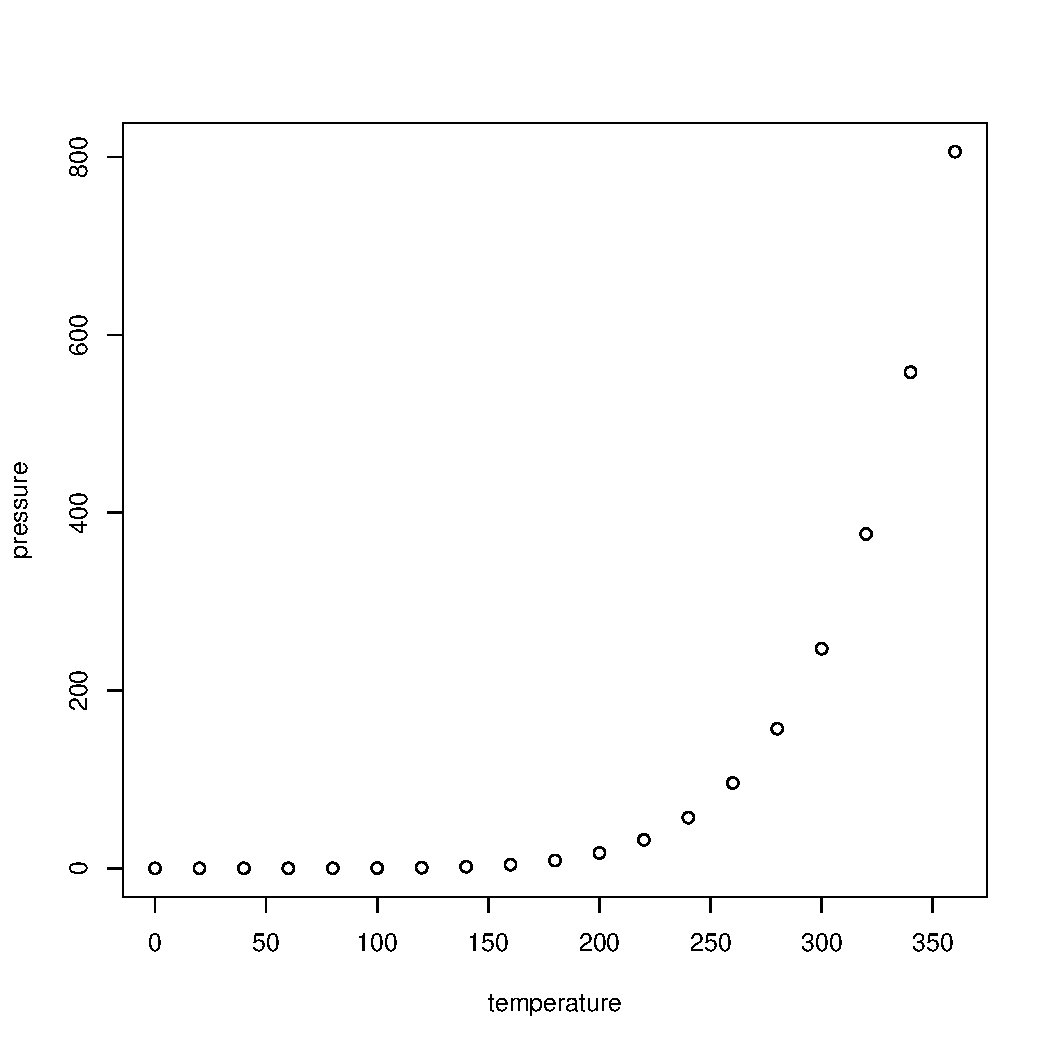
\includegraphics[width=\maxwidth]{figure/fig:pressure-1} 

\end{knitrout}
\caption{Figure Caption...we should turn "echo=False" in the R chunk options, but I left it true for now. (source: ??)} % define the caption, then the label.
\label{fig:pressure}

\end{figure}

\subsubsection{Floating Figures from External Sources}

All figures and images that are imported should be put into the ``images'' sudirectory to keep stuff organized. Even better to create a subdirectory with your images, but we can naviagate as we go.

Figure \ref{fig:vadose} is a good example of inserting an image from an external source.

\begin{figure}
\includegraphics[width=\linewidth]{images/Lee-Vadose}
\caption{Vadose zone is neato (Source: \citet{lee2017fifty}).}
\label{fig:vadose}
\end{figure}

In this case, I had to specify the width so it would fit on the page!  See the Rnw file for the code. Notice, I was also abel to ``reference'' the figure in the text.

\subsection{Adding Citations}

See the Guide, as well, but my video is probably the most helpful.


Generally, there are many environmental trends in Asia \citep{imura2005urban}.

\citet{imura2005urban} describes the how urbanization has affected the hydrology of East Asia. 

\subsection{Adding Glossary Words}

\newglossaryentry{entry}
{
  name={entry},
  description={my entry description.}
}

\gls{entry} is defined in the glossary! 
 

\chapter{Nora's Practice Sessions}

\chapterauthor{Nora}

$\rightarrow$

4/23
1. made new project titled ERTA2020-NewEA30e21-Project
2. did the single branch clone for EA30e21
3. switched the Git brach pull down to EA30e21 in remote: ORIGIN
4. testing if I can push to my branch only 
5. save changes
6. commit - TEST NEW PROJECT PUSH TO BRANCH at 2:04
      did it work? 2:03 est
      YES 2:16 est


1. added Marc's repo as the "upstream" to be able to pull from his branch when things are changed there
2. tried to fetch from marc's EA30e21 branch. - SUCCESSFUL
3. no need to use the "git merge origin EA30e21 "code
4. going to test making a pull request to Marc after saving, committing and pushing to my repo. 
    did it work? 7:45 est
    YES 7:51 est

\section{Testing Various Push and Pull Options}

test commit and pull request 


\subsection{What Factors Drive Land Use Change?}





\mainmatter


\chapter{The Earth System}\label{earthsystem}

\chapterauthor{Marc Los Huertos}

\section{The Sun's Energy and the Earth's Temperature}

The temperture of the Earth's surface is the result of a balance -- the energy entering the atmosphere and the leaving the atmosphere. Most of this energy is in the form of light or electromagnetic radiation (Figure~\ref{fig:earthbudget}). 

\begin{figure}
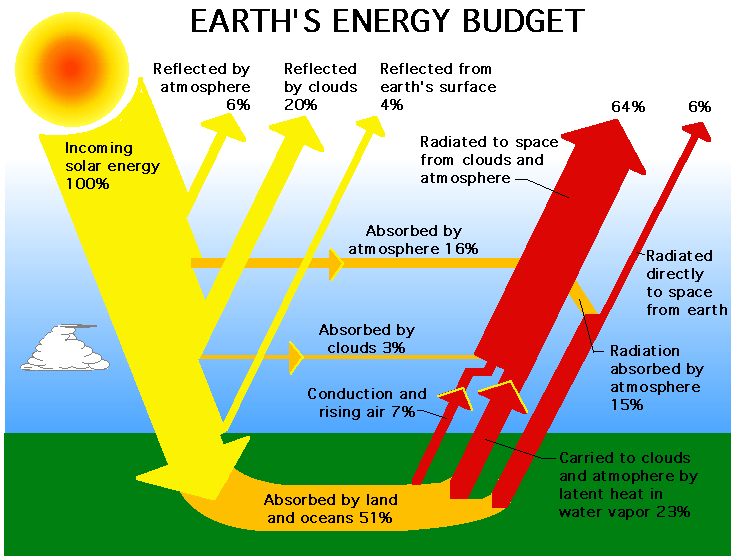
\includegraphics[width=\linewidth]{images/earth-system/earth-rad-budget-nasa-erbe.png}
\caption{caption}
\label{fig:earthbudget}
\end{figure}

Light enters the atmosphere, where some is absorbed and some is reflected. Light interacts in different ways with land, oceans, and vegetation, which is beyond the scope of our project. The ``quality'' of light changes through these processes. 

\subsection{The Spectrum of Light Entering and Exiting the Earth's Surface}

As the sun's electromagnetic radiation interacts with the Earth's Atmosphere, certain wavelengths are absorbed and filtered out (Figure~ \ref{fig:em-entering}).

\begin{figure}
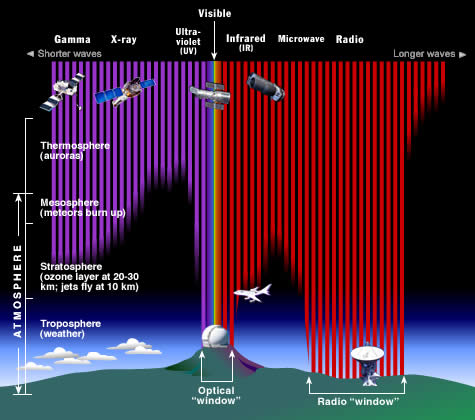
\includegraphics[width=\linewidth]{images/earth-system/em-radiation-atmosph-depth-stsci.jpg}
\caption{Various wavelengths of solar electromagnetic radiation penetrate Earth's atmosphere to various depths. Fortunately for us, all of the high energy X-rays and most UV is filtered out long before it reaches the ground. Much of the infrared radiation is also absorbed by our atmosphere far above our heads. Most radio waves do make it to the ground, along with a narrow `window' of IR, UV, and visible light frequencies. Source: STCI/JHU/NASA.}
\label{fig:em-entering}
\end{figure}

\subsection{The Atmosphere and Greenhouse Effect}



\section{Carbon Biogeochemistry}

\subsection{Long and Short Time Scales}

The carbon cycle processes occur at wide range of temporal scales from hundreds of millions of years to seasons of the year. These have been referred to as long and short carbon cycles. However, for our purposes, I will call them ``geologic carbon'' and ''biosphere carbon'' processes. 

\subsection{Rock Cycle and Geologic Carbon}

The carbon cycle describes changes in the fluxes and reservoirs of carbon in the Earth system. On very long time-scales, millions of years, the primary reservoirs of carbon are the atmosphere, ocean, and rocks (limestone). Carbon moves between these reservoirs through volcanic outgassing, silicate weathering, and limestone sedimentation. The carbon cycle is linked to Earth's energy balance through atmospheric carbon in the form of \carbondioxide, a greenhouse gas.

\subsubsection{Mountains and Erosion}

\ref{fig:carbonpools}

\begin{figure}
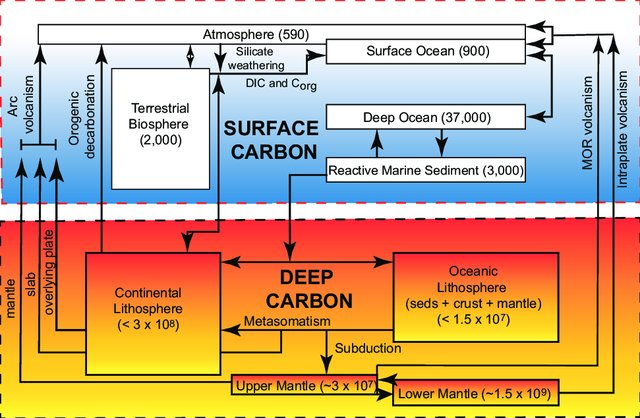
\includegraphics[width=\linewidth]{images/earth-system/Carbon-reservoirs-and-cycles-in-the-Earth.jpg}
\caption{Carbon reservoirs and cycles in the Earth. The figure shows short-and long-term cycles; biosphere and geologic carbon reservoirs and fluxes, and the relative sizes and residence times (y axis) of respective carbon. Numbers in brackets refer to the total mass of carbon in a given reservoir, in Pg C (1Pg C = 10$^{15}$ g carbon). All reservoirs are pre-industrial. Abbreviations: C org = organic carbon; DIC = dissolved inorganic carbon; MOR = mid ocean ridge; seds = sedimentary rocks. Adapted from Lee et al. (2019 And references therein).}
\label{fig:carbonpools}
\end{figure}

\subsubsection{Subduction Burial and Carbon Recycling}

Figure~\ref{fig:longtermcarbon}

\begin{figure}
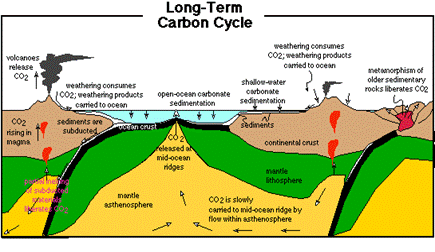
\includegraphics[width=\linewidth]{images/earth-system/long-term-carbon.png}
\caption{Schematic of the long-term carbon cycle (from Bice, 2001)}
\label{longtermcarbon}
\end{figure}

\subsection{Photosynthesis, Respiration, and Biosphere Carbon}

\subsubsection{Soil Respiration and the Soil Profile}

Carbon in soils is respired -- but different pools might have different rates of respiration. Sometimes these pools are distinquished as an active soil organic carbon pool and slow soil organic carbon pool. Although the reference of ``slow'' causes confusion with long-term, geologic carbon, but soil organic carbon remains a component of what we are refering to as biosphere carbon. 

The surface of the soil tends to have more SOC and microbes that can use that carbon for respiration. Lower down in the soil profile, we tend to see lower amounts of SOC and lower microbial biomass (Figure~\ref{fig:soilcarbon}. In addition, soils in the lower part of the profile tend to have more aggregation that protects SOC from microbial attack, thus a key area that soil carbon can seqeustor carbon. 

In addition to these microbial biomass and aggregate patterns, the microbes aree more senstive to temperature changes near the surface as measured by Q10 -- the rate of biochemical processes with a 10 degree C increase in temperature. Thus, soil processes, such as respiration, is likely to increase more near the surface with global warming that the lower part of the soil profile.  

\begin{figure}
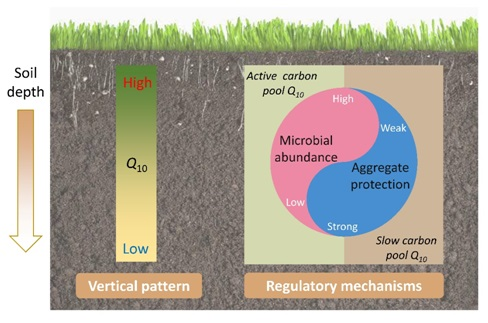
\includegraphics[width=\linewidth]{images/earth-system/Q10-SOC-Regulation.jpg}
\caption{Regulatory Mechanisms of the Temperature Sensitivity of Soil Organic Matter Decomposition in Alpine Grasslands (Source: \citet{Qineaau1218, CAS2021researchers}).}
\label{fig:Q10-SOC}
\end{figure}


\section{Fossil Fuels and Carbon Dioxide Trends}\label{sec:fossilfuels}

As part if the industrial revolution, our energy sources have put more \carbondioxide from the biosphere (soils and forests) and geologic carbon (coal, petroleum). 

\subsection{The Signal of Geologic and Biosphere Carbon in Atmosphere}

The combined contribution from geologic and biosphere carbon in the atmosphere is clearly documented from numerous sources. First, look at data collected at the Mauna Loa where \carbondioxide measurements have been taken continuously since the late 1950s (Figure~\ref{fig:maunaloa2}).

\begin{figure}
\begin{knitrout}
\definecolor{shadecolor}{rgb}{0.969, 0.969, 0.969}\color{fgcolor}
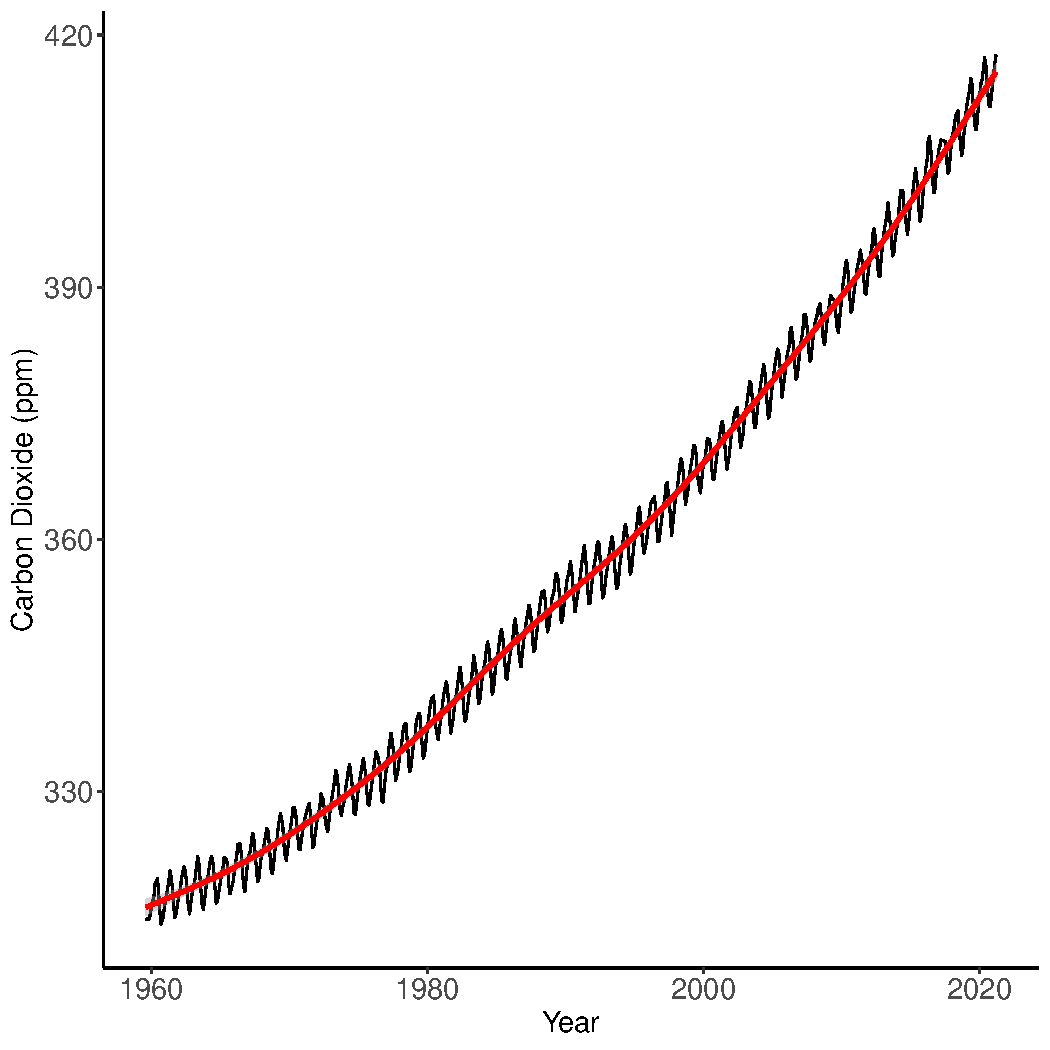
\includegraphics[width=\maxwidth]{figure/maunaloa3-1} 

\end{knitrout}
\caption{Carbon Dioxide Measure on Mauna Loa, HI}
\label{fig:maunaloa2}
\end{figure}






\chapter{Monsoons and East Asia Climates}

\section{Temperature Gradients and Latitude}

\subsection{Monsoon -- Dominant Climate for SE Asia}

Monsoons are identified with copious seasonal rainfall as well as with steady seasonal winds, which reverse their direction in a persistent manner with surprising regularity. The term `monsoon' has its origin in the Arabic word `mausim', which means season. Seamen used this word for many centuries to describe a system of alternating winds over the Indian Ocean and Arabian Seawhich blow from the north-east for six months and from the south-west for the remaining six months. In general, the shift in seasonal wind is about 120$\degree$, which is mainly caused by the differential heating of land and ocean. Monsoon winds are most pronounced in the summer season of either hemisphere. The monsoons blow over East Asia, South Asia, Africa, and northern parts of Australia. Recently the presence of a monsoon has also been recognized over south-western parts of North American continent. Overall, about half the tropics or a quarter of the surface area of the entire globe may be defined as having a monsoon climate.

The annual cycle of the monsoon contains two strong components. One is the summer monsoon, which lasts almost from June to September. The second component, the winter monsoon, lasts roughly from December through February. The summer monsoon in southern Asia is a huge climate system in which the Indian monsoon and the East Asian monsoon are the principal constituents.

For millions of people in monsoon regions, monsoon rainfall is the only accessible source of water. If the monsoon fails, people's lifestyles can be severely disrupted. Accurate prediction of monsoon onset and quantum of monsoon rainfall for a few days up to a season can make a difference between agricultural success and failure. Accurate monsoon forecasts with sufficient lead times are also required for government action and public response. Similarly, prolonged droughts and floods can bring excess hardship to the people in the monsoon region. These may lead to loss of life and property, and a heavy economic burden on the people as well as on the government.



\chapter{Critical Zone}\label{ch:critical-zone}

\chapterauthor{Marc Los Huertos}\footnote{The chapter was first drafted by Marc Los Huertos (2021). The author recieved valuable feedback from X, and Y and Z to improve the chapter.}

\section{What is the Critical Zone}

The crticical zone refers the the portion of the Earth's skin where the zone where rock meets life. The Critical Zone supports all terrestrial life.

The critical zone includes the following:

\begin{itemize}
  \item A permeable layer from the tops of the trees to the bottom of the groundwater;
  \item An environment where rock, soil, water, air, and living organisms interact and shape the Earth's surface;
  \item Water and atmospheric gases move through the porous Critical Zone, and living systems thrive in its surface and subsurface environments, shaped over time by biota, geology, and climate.
\end{itemize}

All this activity transforms rock and biomass into the central component of the Critical Zone - soil; it also creates one of the most heterogenous and complex regions on Earth.

Its complex interactions regulate the natural habitat and determine the availability of life-sustaining resources, such as food production and water quality.

These are but two of the many benefits or services provided by the Critical Zone. Such `Critical-Zone Services' expand upon the benefits provided by ecosystems to also include the coupled hydrologic, geochemical, and geomorphic processes that underpin those ecosystems.

\begin{figure}
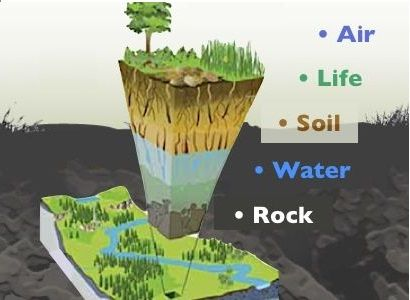
\includegraphics[width=\textwidth]{images/critical-zone/criticalzone.jpg}
\caption{The Critical Zone is an interdisciplinary field of research exploring the interactions among the land surface, vegetation, and water bodies, and extends through the pedosphere, unsaturated vadose zone, and saturated groundwater zone. Critical Zone science is the integration of Earth surface processes (such as landscape evolution, weathering, hydrology, geochemistry, and ecology) at multiple spatial and temporal scales and across anthropogenic gradients. These processes impact mass and energy exchange necessary for biomass productivity, chemical cycling, and water storage.}
\label{fig:criticalzone}
\end{figure}

\subsection{What are the environmental implications of the Critical Zone?}

The critical zone as a concept and as a material space pushes us to think of the porousity of the Earth's surface --- the gas and fluid flows through rocks, soils, and plants. We can begin to appreciate the complexity of the transport and fate of chemical pollutants as they enter the soil and become part of the vadose zone and perhaps the ground water table -- moving with water and diffusing through the water, simultaneously.

\section{Hydrologic Aspects}

\subsection{Subsurface Hydrology}

As water percolates into the soil or flows in the pour space below the surface waters it becomes part of the ground water. The study of this water might be called subsurface hydrology or ground water hydrology or hydrogeology. 

There are two main areas of subsurface waters: saturated zone and unsaturated zone (Figure~\ref{fig:groundwater}).

The saturated zone is the region where all the spaces between the particles are filled by water. The surface of the saturated zone is the water table. 

The unsaturated zone is also called the vadose zone has some percentage of the pour spaces have air. The vadose zone also includes an area called the capillary fringe. Because of the surface tension of water, water is found in between particles above the water table and this zone is referred to as the capillary fringe. 

\begin{figure}
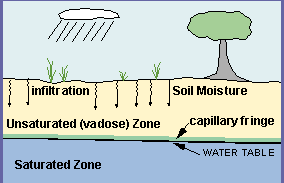
\includegraphics{images/critical-zone/groundwater}
\caption{Diagram of Ground Water. }
\label{fig:groundwater}
\end{figure}

\subsection{Saturated Zone}

\subsubsection{Aquifers and Aquitards}

\subsubsection{Confined and Unconfined Aquifers}

\subsubsection{Ground Water Flow}

TAKE A LOOK at some flow net sketches that will help clarify the relationships between aquifer matrix, and groundwater movement.

In general, water flow is driven by potential energy, e.g.  where water flows down hill, driven by gravity. If water flows from point A to point B, the the potential energy for the flow is the height of the water at point A minus the height at point B, which can be symbolized as $dl$. The head potential is the heigh difference divided by the distance between the two points.  

DARCY'S LAW

\begin{equation}
Q = KIA
\end{equation}

In 1856, Henry Darcy studied the movement of water through porous material. He determined an equation that described groundwater flow. The following description tell how Darcy determined his equation:

A horizontal pipe filled with sand is used to demonstrate Darcy's experiment. Water is applied under pressure through end A, flows through the pipe, and discharges at end B. Water pressure is measured using piezometer tubes (thin vertical pipes installed at each end of the horizontal pipe). The difference in hydraulic head (between points A and B) is dh (change in height). Divide this by the flow length (i.e. the distance between the two tubes), dl, and you get the hydraulic gradient ( I ).

The velocity of groundwater is based on hydraulic conductivity (K), as well as the hydraulic head (I). Therefore, the equation determined by Darcy to describe the basic relationship between subsurface materials and the movement of water through them is Q = KIA where Q is the volumetric flow rate (or discharge) and A is the area that the groundwater is flowing through. This relationship is known as Darcy’s law.

DISCHARGE
%* symbol-Q * units-volume/time EX. (m^3/day) * volume of water flowing through an aquifer per unit time * FIND WITH DARCY'S LAW Q = KIA

AREA OF FLOW
%* symbol-A * units-distance squared EX. (m^2) * Cross-sectional area of flow. (i.e. aquifer width x thickness)

Now, rearrange the equation to Q/A = KI, which is known as the flux (v), which is an apparent velocity. Actual groundwater velocity is lower than that determined by Darcy, and is called Darcy Flux (vx)

FLUX
%* symbol-v * units-distance/time EX. (m/sec) * v=Q/A=KI * this is a velocity measure and gives the IDEAL velocity of groundwater (assumes that the water molecules can flow in a straight line through the subsurface). * this is ideal because it doesn't account for tortuosity of flow paths (this means that the water molecules actually follow a very windy path in an out of the pore spaces and so travel quite a bit slower in reality than the flux would indicate).

DARCY FLUX
%* symbol - vx * units - distance/time EX. (m/sec) * vx = Q/An = KI/n * This is the ACTUAL velocity of qroundwater and DOES account for tortousity of flow paths by including porosity in its calculation.

Darcy's law is used extensively in groundwater studies. It can help answer important questions such as what direction an aquifer pollution plume is moving in, and how fast it is traveling

\subsection{The Vadose Zone}

The vadose zone is the 

Jeji is a volcanic island is located some XX km south of the Korean Penisula. Water runs off the steep slopes quickly and water supplies are limited on the island. To adddress this...\citet{lee2017fifty}.

\begin{figure}
\includegraphics[width=\linewidth]{images/critical-zone/Lee-Vadose.png}
\caption{... (Source: \citep{lee2017fifty}).}
\label{fig:vadose2}
\end{figure}



\chapter[Land Use Change and Monitoring]{Science of Remote Sensing on Biogeochemical Changes to the Land}

\chapterauthor{Samantha Beaton}

\section{Example of a Place: Urbanization and Land Use Change in Shenzhen, China}

Following the late 20th century reform period, China has embarked on a mass urban renewal project, and so it is\red{passive voice} a particularly interesting place to begin analyzing land use change. A study\red{is the study itself important or the results? It can be both, but in the intro, I would avoid jumping into studies per se} analyzing land use change in Shenzhen recorded a significant drop in arable land (covered by grassland or forests) between 1996 to 2006 from 51.36\% to 45.72\% (Qian et al.) (Figure~\ref{fig:shenzhen}). Regardless of potential impacts, it cannot \red{passive voice} be ignored that the land is changing at a rapid pace. This phenomenon, reflected in Figure 1\red{remove reference?}, may be particularly felt in South East Asia, as is the scope of this chapter, but is certainly relevant worldwide. How does land use change affect the environment?

\begin{figure}
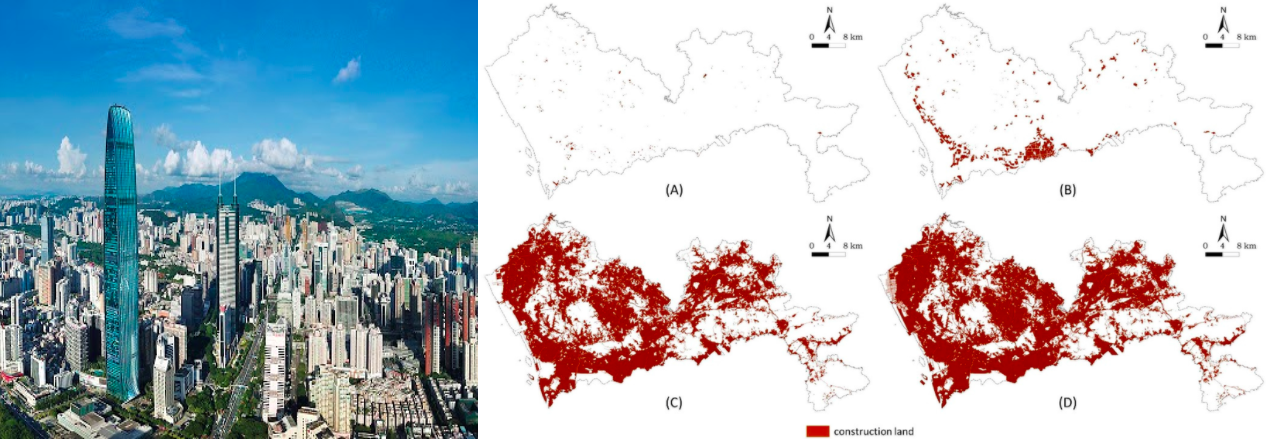
\includegraphics[width=\linewidth]{images/land-use/Shenzhen-cityscape.png}
\caption{(A) Shenzhen cityscape, China. (B) Change in construction land within Shenzhen from 1979, 1986, 2005, and 2014.}
\label{fig:shenzhen}
\end{figure}

As most scholars would agree, we are currently situated in the Anthropocene, \red{I like that you appeal to authority, but can you put this in more nuanced way?} or at least an age dominated by the systems of humans\red{I like this, start here then define anthropocene}. The supposed ''age of man,'' as described by environmental artist and engineer Natalie Jeremijenko,\red{a picture of her work here would be very useful!} asserts how humans are ''major biogeochemical forces in the world.'' By simple definition, humans have a true impact on the land, which then responds. Humans are entangled in the forces of nature. 

An interesting perspective to consider land use change can be situated in a comparison to the body through traditional Chinese medicine (TCM)\red{neat idea, but let's see if we can be more circumspect, and perhaps use evidence then cite this paper?}. In a paper understanding climate change through Qi,  et al.\red{let's work on references this week} describes how climate represents the Qi of nature, the larger body. In this framework, humans act as cells within this body. As with the traditional understanding of the human body, when the dynamic between the cells and body are disrupted, as with one dominating the other, the greater system suffers. Furthermore, in the context of yin-yang, in which two opposite factors are interrelated as one, all actions or changes yield a response. Changing the landscape always yields a response from the environment that can be positive or negative, depending on the action. When humans perform an action disharmonious to natural systems, the responses are negative for the entire body. The big question thus becomes how to impact the environment and live within it ``sustainably,''\red{open quotes are accent in latex... I fixed this one} in a way progressing from our current practices with radical change, deconstructs power systems, and moreover reimagines our relationship with nature.

''Land use changes''\red{fix quotes} encapsulates all the ways that humans change the land, which is particularly fascinating when analyzing highly urbanized spaces, and what that means for the surrounding environment. It goes\red{passive voice} into the discourse of where nature belongs, and how different people experience nature differently. What does nature look like in and around a city? How is the greater environment changed? While land use changes may only be implicated onto local land, they can be a contributing influence to places across the globe. Within the context of South East Asia, this chapter will specifically analyze land use changes through various places to understand its most\red{I wonder if this might not be universally agreed upon?} prominent, intersecting issues.

\section{What is Land Use Change?}

Simply,\red{I don't think we need the Simply} land use changes are the ways in which land is converted or transformed by humans to serve another purpose than its previous. In a largely industrial, capitalist society\red{currently, this is the driver, but that doesn't explain the previous 3000 years before the rise of capitalism and colonialism\ldots }, land conversion is most often described to its economic productive role: land is most often shifted to satisfy agricultural and urban needs. 

\subsection{What Factors Drive Land Use Change?}

Land use changes are influenced by both proximite (direct changes to environment from proximate sources) and underlying (indicative of larger social/biophysical processes that drive change) forces that set certain conditions specific to the place. Underlying forces are largely considered to include economic, policy and institutional, technological, sociopolitical and cultural, demographic factors.\red{can we make a graphic for this?} As used in a study analyzing land-use change across 8 regions in Southeast Asia over 10 years, proximite causes focused on agricultural expansion, wood extraction, and infrastructural development as the main factors, with space for others in a miscellaneous category (Fox and Vogler). In corroboration with previous research, this study\red{how about using authors as subjects?} found that multiple causes contributed to land use change, with agriculture being a common thread. On the underlying level, state policies (especially in relation to climate and property rights) influenced these motivations the strongest, as well as economic market pressures to establish commercial agriculture sites and the general impact of land tenure systems that determine land ownership.\red{super interesting!  nice}

\subsection{How is Land Use Change Measured and Quantified?}

Land use change is primarily measured through \st{processes of}\red{do we need this?} remote sensing. Temporal and spatial data are compiled\red{is this the right word?} from aerial photos, satellite images, and various radar sensing systems to be analyzed into topographic maps and more. It\red{what is `it'?} may also integrate interdisciplinary practices to further understand socioeconomic and institutional factors that affect a given landscape, as well as how that land has changed through history.\red{nice inclusiveness}

\section{The Science, Art, and History of Remote Sensing}

Socrates once wrote: ''\red{quote}Man must rise above the Earth to the top of the atmosphere and beyond, only thus will he fully understand the world in which he lives.'' The science of remote sensing attempts to do just that. The term ''remote sensing'' is attributed to be first officially used in the early 1960s by Evelyn Pruitt, a geographer within the U.S. Office of Naval Research (Fussel et al., 1986)\red{interesting -- a new science is born, in effect, right?}. In short, it is used to describe the science and art of identifying, observing, measuring, and analyzing a target object from a distance without direct contact (NASA, 1999). 

\subsection{Invention of Aerial Photography: Pigeons, Kites, Balloons}

Roots of remote sensing began upon the invention of photography, with one of the first practical processes developed in 1839 by Louis Daguerre in France (Moore, 1979). Aerial photography (that was also full-spectrum-sensitive) can be traced back to 1868 when Nadar aka Gaspard-Félix Tournachon captured the first from aboard a hot air balloon (Salomonson, 2015). From then, aerial photography was captured with cameras attached to pigeons, kites, and even more balloons. By the year 1909, the first photograph was finally taken from an airplane (HSU, 2019). \red{super interesting}

\subsection{Remote Sensing in the Early-to-Mid 20th Century and Military Reconnaissance}

Soon after, aerial photography was quickly taken up by the U.S. military for various reconnaissance purposes. The progressive development of aerial photography is deeply tied to military advances and demands beginning during World War I when cameras were mounted to German and American aircrafts to monitor positions of troops (Salomonson, 2015).\red{what were the first uses in Asia?} In 1918, it was\red{passive voice} recorded that the French military in particular captured and developed up to 10,000 photos per day from such camera mounts (Moore, 1979).\red{you can use moore here as the topic of the paragraph and then don't need to cite him in every sentance} During World War II, non-photographic remote sensing methodologies were developed using radar (radio detection/ranging), thermal infra-red detection, and sonor (sound navigation) systems (Moore, 1979). In particular, radar systems were developed by Britain and the U.S. to track ships and aircrafts (Salomonson, 2015).\red{as part of war efforts, thus explain why asia didn't have this??} In the 1950s, the University of Michigan spearheaded development of other systems including infrared radar and synthetic aperture radar (SAR) imagery, which was used (and later declassified) during the 1960s in experimental programs by the U.S. National Reconnaissance Office (Salomonson, 2015; Xiao et al., 2019). \red{and in Russia?}

\subsection{Satellites in Space: Remotely Sensed Earth Observations}

The beginning of remote sensing from space began with V-2 rockets, the first long-range missiles developed during World War II (Salomonson, 2015). As the late 1940s saw the end of WWII and the very beginnings of the Cold War, the Soviet Union and U.S. both took advantage of captured V-2 rockets to start research and development on launch vehicles for space programs (Britannica). While the first picture taken of Earth from the sky (high enough to see its curvature) was captured in 1935 on a balloon 13.7 miles high, it was in March of 1947 when a camera placed in the nose shell of a V-2 rocket flew more than 100 miles above ground; once the series of pictures were stitched together, it clearly showed for the first time Earth against the black space, spanning more than a million miles together (NASA, 2017).\red{oh, this is cool, how about some impages for each of these sections above to illustrate what you are talking about?} It was these pictures that set the stage for the potential of remote sensing to be used to monitor Earth’s processes. Still, it was not until the mass development and launching of various satellites during the Space Race when this prospect was cemented as reality.

In 1957,\red{good} the Soviet Union launched the first satellite into space, the Sputnik 1, with the U.S. following shortly behind (HSU, 2019). In 1964, photographs obtained from the Mercury-4 spacecraft were recognized as highly-valuable to understanding Earth sciences (Moore, 1979).\red{can we see this image} National institutions aside from NASA, such as the U.S. Department of Agriculture (USDA), U.S. Geological Survey (USGS), and National Oceanic and Atmospheric Administration (NOAA) all realized the potential application of remote sensing to fields of agriculture, hydrology, archaeology, geography, oceanography, and meteorology (Bauer, 2019). In 1960, NASA launched its first low-orbital experimental weather satellite, the TIROS-1, who’s success proved the feasibility of capturing images of Earth from space (NASA, 2017). Thus welcomed the 1968 development of the Earth Resources Technology Satellite series, now called LANDSAT, sent to record worldwide images on a continual basis--a series that has continued ever since (Moore, 1979). From these developments, images would from then on not only be turned towards enemy troops, nor towards space, but also towards the Earth--the beginning of modern remote sensing.\red{This is great stuff -- as a history goes, but I wonder if you could put East Asia in here more... even if the 'subject' of military surveilience (sp?).}

\subsection{Critical Remote Sensing}

Still, the history of remote sensing cannot be understood without analyzing its use in producing and controlling knowledge to monitor and manage global resources and populations. After all, the purpose behind remote sensing is deeply tied to map-making and cartography, which itself has a fundamentally colonial history. During the Western world’s\red{fix apostrophe} Age of Exploration, or Age of Information, between the 15th and 18th centuries, Europe financed global expeditions not only to conquer and colonize, but to gather information on the land’s resources and people (Bennet, 2020). In this way, maps were used to classify life for the purposes of exploitations. They were used to mark territory, regardless of local dynamics, for the use of settlers. Maps, then, were essential to the imperialist settler colonial state in dominating a land. As noted by University of Hong Kong Geography professor Mia Bennet, the quest for information is ''an activity critical to empire'' (Bennet, 2020).\red{great, and if you can link to SE Asia colonialism too...} If so, what then must be true to our current quest for information? What must we be critical of if remote sensing is just another rendition, albeit modernized, version of the colonizing tactics of those in power?

Additionally, a key component to colonial mapmaking was the arbitrary creation of boundaries. Remote sensing analyses can fall into a similar ''territorial trap'' that disregards how human activities, resources, and environmental change occurs as natural flows that transcend transnational boundaries (Bennett, 2020). By working within discrete state boundaries, data and resulting maps can reproduce certain narratives, particularly ones that suppress developing countries over developed ones.\red{nation building?} We can see this in the map below (Figure 2)\red{ref figure using latex command} on soil erosion rates and vulnerabilities across the globe, dictated by national boundaries. While developing countries are illustrated in red, indicating high rates of soil erosion and land degradation, developed Western countries look perfectly clean. This example is just one in a long line of historical misrepresentations of local occurrences that are ever-more complex than what can (and molded to) be portrayed in bordered images. Systems of remote sensing must strive to actively dismantle the colonial, militaristic foundation it is so strongly built upon.\red{great point -- which is a history of advances in Remote Sensing in total\ldots}

Figure~\ref{fig:Bonelli Erosion Map}\red{I generally put a tilde in between the ref and Fig because is make a "prettier" spacing}

\begin{figure}
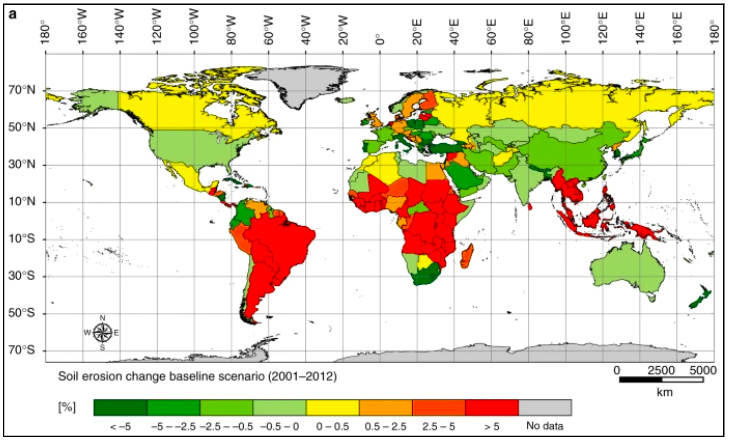
\includegraphics[width=\linewidth]{images/land-use/Bonelli_Erosion_Map.png}
\caption{Global land use change and soil erosion estimates, measured on a scale of severity by colors green (low erosion risk) to red (high erosion risk). As denoted by the red color, Southeast Asia is expected to experience a higher risk of soil erosion compared to other regions in the world (Borelli, et al.).}
\label{fig:Bonelli Erosion Map}
\end{figure}

In an analysis of China’s ''One Belt, One Road'' policy (aka the Belt and Road Initiative or BRI), which as of 2019 lacked an official map shifting the focus to governmental remote sensing illustrations for accountability of the policy’s efficacy, Bennet importantly points out an illusory distinction between traditional maps and those obtained through remote sensing: ''Whereas maps are considered malleable representations, satellite imagery is imagined as objective, neutral, and importantly, rational—a key word in Chinese narratives of development and modernization.''\red{wow, this is really important! nice job, perhaps make this more prominent?} In other words, while remote sensing may easily be seen as perfectly objective, it in fact requires interpretation and representation, so it too is\red{awk} inherently political. While the goal of remote sensing is to accurately capture reality, the ''processing of billions of pixels'' can just as easily be edited or reframed to \red{“}help turn policies into self-fulfilling prophecies” (Bennett, 2020). Remote sensing produces entire analyses of landscape that may look ‘rational’ or ‘self-evident’; the challenge thus requires a critical look into each trillion pixels and the spaces left unattended within its representation.

Bennett thus presents a methodology of three main principles to foster critical remote sensing:
\begin{enumerate}
\item Any analysis must ``be sensitive to the (geo)politics involved in the production and analysis of satellite imagery'' by looking closely at the motivations of goals of the controlling state
\item Analysis should not conform but rather act to contest ``dominant social meta-narratives and discourses about modernization and development'' that often use sensing to sustain development and paint a `pretty' picture of modernization. Critical remote sensing includings the encouragement of political debate.
\item Sensing should include mixed methods of qualitative and quantitative analysis at various research scales and levels throughout its production.
\end{enumerate}

Ultimately, the increased use of remote sensing systems within government agendas and policy initiatives requires the need for active critique on the politics and positionalities ingrained in satellite imagery, especially due to how ''images present the guise of the entire truth in a way that can dissuade debate'' (Bennet, 2020). Data must be transparent, management must be accessible, and analysis must be critical to rightly expose the complexities of the (sociopolitical) environment. Lastly, while remote sensing is without a doubt an advantageous to our modern society, it cannot entirely replace local observation and place-based understanding, but rather is best kept in balance.

One further point of hindrance to a more fair and just remote sensing system is that the large majority of imaging satellites currently being used are operated and controlled by the most powerful of countries. Increased participation in remote sensing can be created by giving smaller states, organizations, and universities the opportunity to launch their own satellites rather than needing to depend on powerful governments: a ''democratization of space'' (Bennett, 2020). While this potential is increasing in actuality, it is far from truly increasing representation. Still, it was promising in 2008 when the USGS decided to make all LANDSAT records available to the public for free, when previously it was kept behind a paywall (Xiao et al., 2019).\red{what were the political reason for this?} As remote sensing becomes increasingly popular, it is also increasingly common for data to be released and available to the global public. Using this available data, researchers, scientists, and the public are dedicating more time to analyzing ecological effects of land use change within Earth's systems. It is a\red{passive voice} practice becoming evidently more important as land degradation and desertification intensifies, necessitating directive action with transparent sources of data.

\section{Ecological Effects of Land Use Change on Soil, Air, and Water}

Land use change is associated with deforestation and the general destruction of land (at least the land that existed upon conversion), and is thus the biggest driver in terrestrial biodiversity loss. What other long-term impacts does land use change have on the environment, especially when the land is converted into agricultural or urban spaces?

Land use change is the encroachment into habitat for greater space, whether for farmland or urbanization, and so is therefore acted upon through deforestation. By replacing native vegetation with crops or buildings, the soil degrades, suffering a loss of stability that the vegetation provided. It is for this reason that anthropogenic land use change is the primary accelerant of soil erosion. Forests, by far, hold the lowest soil erosion value, certainly in comparison to semi-natural and cropland vegetation (Bonelli, et al.). Additionally, uprooting the land and changing its function creates  a loss potential for carbon sequestration. It is estimated that approximately 12.5\% to 17\% of carbon emissions have originated from loss during land use and land cover changes (Houghton, et al., Paustian, et al.).\red{great points, let's see if we can more succinct}

\subsection{An Introduction to Land Use Change}

\subsubsection{types of data source??}

perhaps some type of intro to the categories coming... even an illustration might be useful. 

\subsubsection{Soil Classification}\red{I suggest we put this in the critical zone chapter and then you can reference that\ldots}

Soil is the combination of biotic organisms and dirt—it is the thick, rich, brown substance that gives rise to life on earth. Soil also exists as layers, divided generally into five horizons. The first layer is the O horizon where organic matter such as plant residue accumulates (NRCS, 2010). Decomposing material mixes with dark nutrient-rich mineral soil in the A horizon (Montgomery, 2007). Layers O and A characterize the topsoil where most plant activity takes place as well as weathering processes and erosion, so it is the layers of soil most relevant to land use change. The first layer within the subsoil is the B horizon where the soil is generally thicker and denser with less organic content; leached materials and minerals from above also accumulate here (Montgomery, 2007). The subsequent C horizon contains older materials than those above it, and overlies the lowest R horizon which makes up the bedrock (NRCS, 2010). Again, the topmost layers of soil have the greatest relevance to agriculture and land use change.

\subsubsection{Weathering, Soil Formation, and Erosion}

Soil is a function of five main environmental factors: 1) regional climate, taking into account average temperature and precipitation 2) topography that describes the landscape shape and slope 3) parent material from which the soil has formed 4) organisms and 5) time (Birkeland, 1999). Aside from basic geology of the landscape, topography in particular—proximity to the water table, degree of slope, etc.— can help predict the effects of weathering that the soil may take from the other factors.

Rocks and soils at Earth’s surface represent two stories: an original formation and a secondary breakdown. Weathering describes this secondary breakdown which, like soil formation, is similarly dependent upon climate, parent material composition, biotic influences, and other factors. It is “the process of rock and mineral alteration to more stable forms under the variable conditions of moisture, temperature, and biological activity that prevail at the surface” (Birkeland, 1999). Physical or mechanical weathering breaks rocks into smaller pieces. Chemical weathering breaks rock or soil bonds at the atomic level i.e. through dissolution (polarity of water molecules pull apart atoms), oxidation, hydrolysis, and other biological reactions (Wiese, 2019). Both physical and chemical weathering processes occur simultaneously in reinforcing each other, and biological activity from plants, microorganisms, or other animals work to increase those processes. The products of weathering contribute to soil profiles. Through chemical processes, released ions may participate in further synthesis or may be removed from the soil environment via transportation of the dissolving water (Birkeland, 1999). If the environment has high levels of aluminum, silica, or oxygen, they could hydrolyze with water to form various types of clay (Wiese, 2019). The resulting soil composition, ever dynamic, depends in large part on the elements, minerals, structures of those elements, and the interactions of those particles with the greater environment. Soil is thus characterized by the rocks from which it is formed, which in term became available via weathering.

Erosion is the natural removal of weathered debris by agents including water, wind, glaciers, or simple gravity (Wiese, 2019). In replacement of the lost mass, new rock rises up bringing with it essential minerals that replenish the soil and further parent material can be deposited from elsewhere. In the words of Montgomery, 2007, the ''soil regulates the transfer of elements from inside the earth to the surrounding atmosphere. Life needs erosion to keep refreshing the soil'' (p.16). In this way, soil integrity is dependent upon weathering and deposition to replenish its nutrient stocks.

Soil will develop withstanding weathering, that is, until the rate of erosion exceeds the rate of soil formation (Birkeland, 1999; Montgomery, 2007). In general, erosion increases with steepness of slopes, sparser vegetation holding the ground, and greater precipitation that all work to weather the soil/rock surface. As described by Montgomery, 2007, landscapes can often get caught in positive feedback loops of erosion, particularly if human influences are involved: when vegetation is removed exposing bare soil, precipitation can more rapidly and forcefully erode soil, reaching deeper to denser layers unable to absorb water, thus increasing runoff and ever more rapid stripping of the topsoil. This phenomenon can of course be compounded by the type of soil being eroded and human influences acting upon it.\red{I think we can put this in the critical zone chapter and then you can jump into source of impacts\ldots what do you think?}

\subsection{Impacts of Agriculture on Soil, Air, and Hydrological Cycles}

\subsubsection{Industrialized Monoculture in the 20th Century}
The thin topsoil layer that covers Earth’s land feeds the world is the foundation of a thriving civilization, yet due to intensive and extensive land use, is experiencing massive risk of degradation and erosion. Big-ag systems of monoculture have been driven by advanced farming technology in response to rising food demands and growing populations worldwide.\red{what is the percent of land use in monocrops?} Induction of high-yielding varieties of crops, including wheat and rice, that require chemical fertilizers and pesticide has also been a defining feature of this age. This intensive, tillage-based agricultural system is associated with many long-term negative ecological impacts, including: a decrease in soil organic matter, biodiversity, nutrient-use efficiency, and water table level, as well as an increase in soil erosion risk, soil quality degradation, groundwater pollution, air pollution, and greenhouse gas (GHG) emissions. Since most land use change is associated with agriculture, the understanding of intensive systems and the promotion of alternatives is an imperative facet to this discussion.

\subsubsection{Soil and Carbon Nutrient Cycling}\red{we can put this in the long and short carbon cycle that I started in the the critical zone chapter}
Carbon is the foundation to life on Earth and is an imperative global cycle, especially in soil where twice as much carbon exists compared to the atmosphere (FAO; Batjes and Sombroek, 1997). Carbon stocks are maintained in an important balance between inputs and outputs with significant implications to the production of atmospheric carbon dioxide. This is important to land use change because the biggest negative driver to soil carbon loss is land-use change (Poeplau et al., 2011). Following industrial processes and fossil fuel combustion, land use change is the second largest contributor to global greenhouse gases (EPA). Land use change is thus an imperative process to consider in analyzing threats to carbon cycles balances.\red{can we get a figure for this?}

Moreover, understanding shifting land uses on carbon cycling is important to understand nutrient stock dynamics. Due to growing socioeconomic pressures, natural vegetation cover has been steadily decreasing. More and more, forest and grasslands are extensively and intensively being converted to agricultural lands or other urban needs, while reforestation projects are also growing in popularity. Poeplau et al., 2011 reviewed shifting carbon stocks in soil following five different types of land use change types across nearly 350 sites in the temperate zone, in which China and much of Eastern Asia resides. Unsurprisingly, complete deforestation resulted in a -32±20\% decrease in equilibrium SOC over 23 years, and grassland to cropland similarly resulted in a -36±5\% equilibrium decrease after 17 years. These numbers in particular reflect the relative vulnerability of topsoil to intensive change.\red{I think this is super interesting, but we'll need to make a direct connection to earlier sections, remote sensing history, or methods or about critical evaluation of the good and bad in these data\ldots}

Figure \ref{fig:LUC-SOC-Table}

\begin{figure}
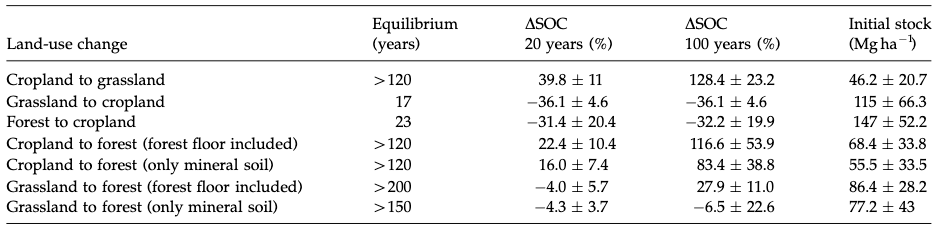
\includegraphics[width=\linewidth]{images/land-use/LUC-SOC-Table.png}
\caption{Comparison of land use change types on years to reach equilibrium, predicted change rates of soil organic carbon stock after 20 and 100 years, and average initial stock value (Poeplau et al., 2011). Note the rapid rates of deforestation (values 17 and 23) compared to longer predicted rates of reforestation land use changes.}
\label{fig:LUC-SOC-Table}
\end{figure}

In comparison with other land use change transitions, restoration of grasslands has one of the greatest potentials for carbon stock restoration. As displayed in Figure 4, shifting croplands to grasslands can result in a 128±23\% increase in SOC—grasslands in particular are long-lasting nutrient sinks (Poeplau et al., 2011).\ref{what is the trade-off?} This is due in part to how grasses form extensive fine root systems. Decomposing roots are considered to be major contributors to organic biomass in soil, further bolstering nutrient loads (Wei et al., 2009). While land degradation and loss of carbon can be a relatively rapid process compared to longer rates of restoration, native grassland restoration at least presents a big potential for successful carbon sequestration, especially in comparison to other land use transitions.

\subsubsection{Shifting Practices}
Still, global populations depend on agricultural land: shifting land practices even if for agricultural purposes is important. More and more studies are providing evidence for both economic and environmental potentials in shifting management practices to return to a more regenerative strategy. This is particularly important in a region like Northeast China where the land provides 30\% of total national maize production for a crop already being one of the biggest food crops in the country. Differences in production potentials can be measured by yield: potential yield is the theoretical ``\red{I fixed opening quote}ceiling” yield for a given place, partially dependent upon its specific environmental conditions, under perfect management. In general, the yield gap between the potential and actual is usually constrained by 1) non-controllable factors (i.e. environmental conditions, access to technology) 2) agronomic and 3) socioeconomic factors (Liu et al., 2016). Compared to other areas of improvement, such as chosen crop variety, the largest potential for increased yield is found to be associated with management practices. These practices move away from intensive systems towards regenerative or conservationist strategies, including the incorporation of crop residue and low-to-no-till practices that combat shallow topsoil.

An increasing demand in maize and rice not only exists  in China but largely South East Asia within the continent, in part due to growing populations and the dependence on such crops\red{let's see if we can make this sentence less complex}. According to some studies, rice production in particular needs to increase an estimated 42\% by 2050 to meet rising global demands (Ray, et al.). \red{maybe a new paragraph?} One of the biggest biotic constraints on actual yields are diseases and pests, including root-parasitic nematodes. Suong et al., 2019 contrasted conventional plough-based tillage rice farming practices to a direct-seeding mulch-based rice cropping system (described closely to practices of regenerative agriculture) based on population densities of root-parasitic nematodes. They found that while nematode population densities were significantly higher in the regenerative system than the conventional system, the rice yields were still higher. These results\ref{can we do a figure to help explain this?} thus show how regenerative systems improve soil fertility and quality both for more productive plants and microbial communities; the higher-nutrient-dense soil not only provided a better environment for microbial biodiversity and nematofauna, but it was moreover productive enough to compensate for any plant damage from the nematodes. These results add to the immense body of research and knowledge that the level of microbidoviersity is a key indicator for soil health. Any land use system that supports this life, then, is most beneficial and sustainable.

Sustainable, regenerative, conservation, or permaculture-based land systems are all names for a common approach in using the land.\red{do these show up in remote sensing analyses?} This approach has the potential to not only ensure food security, but most importantly, has the ability to sustain soil health, promote carbon sequestration (along with other nutrients), decrease GHG emissions, and protect functional ecosystems that then can provide humanity various services. Regenerative agriculture presents an alternative approach characterized by no-to-minimal soil disturbance, diverse crop rotation, and residue retention to enhance nutrient cycling. In short, this integrated, holistic management of land is meant to mimic the natural world—rather than interfere with intensive systems, it is meant to work with existing natural systems.\red{I have some more resources for this that you might find useful}.

''The art of agriculture is a sacred act of collaboration between heaven, earth, and humanity for the production of life-sustaining food.'' —Torizo Kurosawa

Figure \ref{fig:Climate-Smart-Soils}

\begin{figure}
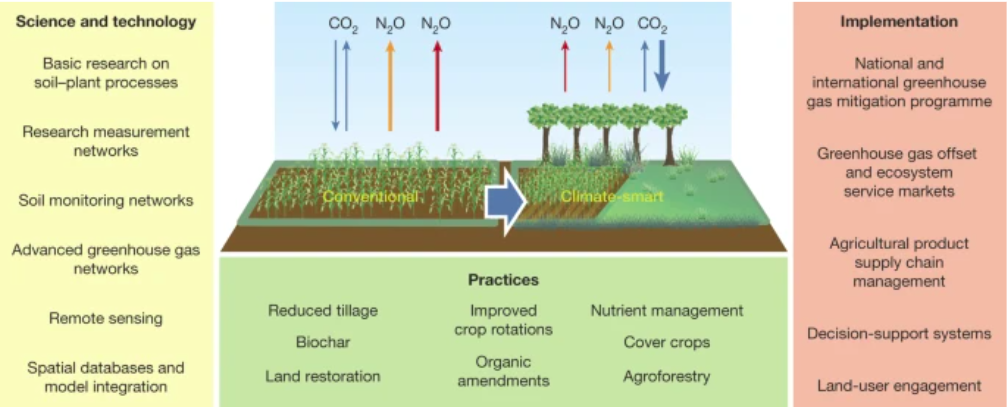
\includegraphics[width=\linewidth]{images/land-use/Climate-Smart-Soils.png}
\caption{Integrated strategy of scientific research, management practices, and widespread implementation of GHG-mitigation-driven agricultural systems (Paustian et al., 2019).}
\label{fig:Climate-Smart-Soils}
\end{figure}

Direct impacts on soil: enhances water infiltration/retention, aeration, structure, porosity → \red{$\rightarrow$} these conditions naturally promote robust root growth, easy nutrient cycling, carbon sequestration (specific values of course vary across climates and soil types)

Enhances microbial biomass and activity: essential to biogeochemical cycling and providing nutrients to plants (essential symbiotic relationships)

Conversely, intensive tillage practices destroy soil ecosystems via changing soil structure, interfering with nutrient dynamics, and altering the soil habitat\red{we'll need to describe these a bit more\ldots}

\subsubsection{Impacts on Local Watersheds}
Land-use changes can alter hydrology of land i.e. infiltration/pollution, groundwater recharge, flow of river basins, runoff
Higher risk of flooding and droughts\red{link to remote sensing?}

\section{Regeneration Efforts in the Loess Plateau, China}

Due to its long history within northeastern China, the Loess Plateau is an apt case study to analyze how a place so important to humanity is related to soil degradation, land management, the potential for restoration, and how to critically go about such a process.

\subsection{The Cradle of Eastern Civilization}

The Loess Plateau, with agriculture beginning in the region nearly 7000 years ago, was once the cradle of Chinese civilization. It receives its name from the loose, porous, easy-to-farm sedimentary deposits originating from the Gobi Desert that define the region. Covering approximately 640,000 sq km, the Loess Plateau was also once the largest distribution of such fertile soil on Earth.\red{good place for a map?}

However, due to intense human activity in the past 2500 years (largely agriculture as well as social conflicts), the high flat plain has experienced severe erosion, transforming it into a land marked by steep, barren hills and deep-cutting ravines. Agricultural processes led to the overgrazing of land that, over a very long period of time, damaged the vegetation. Without trees or plants rooted in the earth, water no longer seeped into the soil but rather evaporated immediately or slid off the hillsides\red{usually don't think of water as sliding\ldots}, eroding massive amounts of topsoil away with it. The land of the plateau eroded seasonally, both by wind and water (Xiao et al., 2009). Over time, \st{massive amounts of}{\red{defin "massive amounts"} silt swept into the Yellow River (thus giving the river its distinct name), with an estimation of 90\% river sediment originating from Loess Plateau erosion, hence the name of the river. Due to lack of water retention, this phenomenon contributed to increased flooding events: as quickly as water would come, it would just as quickly go away so that the region experienced severe droughts. While this is all true, it must be kept in balance with the knowledge that the Loess Plateau was, for thousands of years, a place that built civilization. Generations of people who lived within the region, a center for traditional pastoral life,\red{nomads, I assume?} gave and received a great deal from the soil. The longstanding history of humanity within the region should not be taken for granted beneath the landscape we may see today.\red{try to avoid relative times\ldots, ``in the early part of the 21st Century''?}

\subsection{Beginnings of Modern-Day Restoration}

Beginning in the 1960s, mass efforts have been made to restore the Loess Plateau. After all, one must only look to the neighboring provinces with rich environments,\red{how does one look and see this? not obvious to me how\ldots, perhaps with remote sensing?} such as Sichuan, to realize the potential of such efforts. The primary goal of these endeavors were, and continue to be, increase biomass and biodiversity in all ways within the environment. Methods include terracing of the hills that level out parts of the steep slopes, natural vegetation rehabilitation to restore soil productivity, and additional efforts in check dams for sediment control. A study analyzing the Loess Plateau rehabilitation reflected a trend of increased retention of water in the land, especially since 2000, seen through decreased streamflow and sediment concentration into the Yellow River. (have to regain access to the article—will input figures and explanations of the science here)\red{great!}. While restoration is actively being worked upon on a comparatively small area in the big region, the Loess Plateau rehabilitation effort is representative of the true potential to restore massively degraded land from harmful land usage (Figure~\ref{fig:Loess-Comparison}).

\begin{figure}
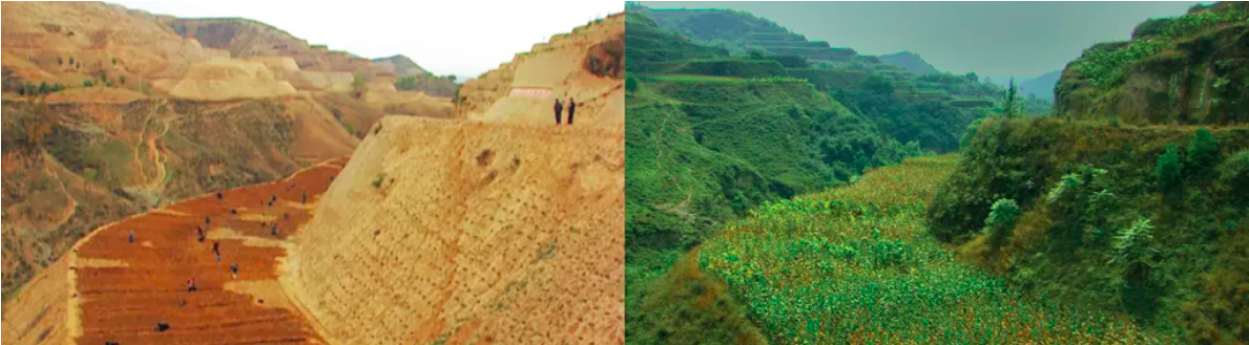
\includegraphics[width=\linewidth]{images/land-use/Loess-Comparison.png}
\caption{Comparison of Loess Plateau from 1995 to 2009 (Liu).}
\label{fig:Loess-Comparison}
\end{figure}

\subsection{Importance of Grasslands and Cautions Against Afforestation}
The Loess Plateau and its unique (yet universal) history of land degradation highlights the importance of maintaining native habitats, particularly grassland ecosystems. Historically, the Loess Plateau was dominated by a grassland ecosystem with the most common native grasses including bunge needlegrass (Stipa bungeana) and Dahurian bush clover (Lespedeza daurica) (Wei et al., 2009). Beginning predominantly in the 1970s when the push to ''green slopes'' reached its highest point in political agendas, large populations of non-grassland vegetation were introduced to reduce erosion. Some of the most popular included the Chinese Pine (Pine armandii)  and Korshinsk Peashrub (Caragna korshinskii) (Wei et al., 2009).

In a study comparing the soil organic carbon, nitrogen, and phosphorous stocks of native grassland and implanted woody ecosystems dominated by the pine and peashrub, Wei et al., 2009 found that the soil of native grass exhibited the highest concentration of SOC and nitrogen stocks. While much of the rhetoric surrounding the \red{“}fight” against desertification centers around reforestation, regeneration of grasslands, especially if it is the historically native ecosystem, can be overlooked at least in predominant media. Still, especially in the Loess Plateau, native grasslands are the ecosystems that generally hold a greater potential for carbon and nitrogen stocks, contributing to more productive soil. Ultimately, grassland root systems play an essential role in nutrient cycling and stocks within soil of the Loess Plateau, and are thus an important measure to consider in relation to land use change.\red{could this be in a figure?}

\section{How GIS Can Be Used to Inform Loess Plateau Restoration}

Just as the ecosystems it attempts to restore, regeneration efforts like that being done in the Plateau are different everywhere. Processes must consider the historical, natural habitat and current conditions—an area made possible in using remote sensing. Remote sensing can be used to develop a site history or a place, an especially important tactic when dealing with projects involving development or restoration. Remote sensing can be used to assess an ecosystem and its soil surface conditions, local hydrology, nutrient cycles, vegetation, and overall geology (Abdullah et al., 2015). Especially in terms of restoration sites, remote sensing can be used to identify reference sites with similar characteristics to further evaluate the target site, thus contributing to a more robust directive towards proper objectives, plans, and action. This was done in modern studies of the Loess Plateau in comparing it to its neighboring region of Sichuan which hosts a rich, lush ecosystem of vegetation and biota. Monitoring is, of course, also important to keep track of long-term changes in vegetation cover and efficacy of restoration methods.\red{I wonder if you can outline a research project and what imagery one would need to conduct this?}




\section{Conclusion \& Prospect of Sustainable Urbanization/Land Use Change}


\chapter{Deforestation}\label{ch:deforestation}

\chapterauthor{Xinlan Chen}

\footnote{Statement of Contributions-- For example, ``The chapter was first drafted by Marc Los Huertos (2021). The author recieved valuable feedback from X, and Y and Z to improve the chapter. Slater revised the chapter in 2022 with suggestions from Cater.'' Note: I am still working on the formatting for this to improve it.}

\red{I added my comments from before, it looks like you didn't get them. Be sure to pull my changes}.


\section{Overall}\red{not a very descriptive heading\ldots}

Deforestation is not a small issue in East Asia, since most countries here depend on the money source they got from the wood export industry.\red{I like this as a start} There are\red{let's see if we can avoid passive voice} many issues that could be caused by deforestation with but not limited to air pollution, water pollution and climate change. Upon having looked at all the presentations that people make, I realized that most East Asia countries that was originally covered mostly in forest have significantly reduced in their forest coverage,\red{let's see if we can find some data on forest changes over the last 200+ years} and nevertheless, natural is punishing\red{interesting, let's see if we can define this} them for that. Over-logging is when the level of deforestation exceeds the self-sustaining state of the ecosystem, leading to desertification\red{important concept, let's see if we can define this too}. Excessive cutting of trees can bring a series of troubles and problems. Many countries have started having regulations on business regarding wood exports and forests protection, more have to be done in order to resolve the issue that people have done in the past that resulted in deforestation. \red{as a road map this intro is very nicely structured}

\section{Damage Done by Deforestation – Example of China}

After soil erosion and deforestation\red{let's see how we can use the land use chapter as a basis / foundation for this section}, the bare land cannot withstand the wind and rain. On sunny days, due to the sun exposure, the ground temperature rises, the process of organic matter decomposition into soluble mineral elements is accelerated;\red{great, let's see if we can make a figure for this\ldots} On rainy days, rainwater is washed directly, carrying the fertile topsoil along with mineral elements into rivers.\red{great! and let's see if we can connect to the processed described in the land use chapter so we are not repeating ourselves.} It is \red{passive voice}estimated that more than 5 billion tons of soil are washed into rivers in China every year\red{how do we know if this it alot or too much?}. The siltation of quicksand\red{?} blocked the channel of the reservoir. Sediment concentration in the Yellow River in China is the highest in the world, and when floods come, water and sand are equally divided. Due to the deposition of quicksand\red{I don't think we mean quicksand}, the riverbed in some places in the lower reaches of the Yellow River is 12 meters higher than the land beyond the embankment and even higher than the city wall of Kaifeng City, posing a serious threat to the safety of people's lives and property.\red{to make a paragraph break, just add a line space\ldots}

The deteriorate of environment always accompanies with frequent disasters. The forest coverage rate in Wanning County, Hainan Province, used to be as high as 63 percent.\red{can we map the changes?} Due to forest regulation, there was no drought in the 1940s and 1950s. Since then, natural disasters have been on the rise. From the 1960s to the 1970s, droughts hit an average of six out of every ten years, cutting the flow of 21 rivers, reducing the output of three-quarters of farmland and drying up 25 reservoirs.\red{super interesting!}  In particular, the destruction of the forest, so that some rare animals lost their breeding base\red{let's cite some examples}. Animals there can't survive. China's Hainan slope deer, South China tiger, black - crested gibbon and other precious animals are endangered due to habitat destruction\red{yes, here they are!  nice, I wonder if we can get these into the previous sentance?}. There is less oxygen supply when deforestation issue is present\red{the atmosphere is 21\%, is there any evidence that O2 is impacted?}, consequently there is more carbon dioxide \red{how is this created?} and less natural filters \red{agreed, but we might need to explain this to our readers}. The ecological environment was forcibly occupied, and the law of ecological circulation was destroyed. The temperature can change, causing unstable changes in the climate.

\section{Overall Losses – Example of Indonesia and Thailand}

In the past decade, Southeast Asia has suffered the greatest loss of forest area, with a net loss of more than 900,000 hectares a year.\red{wow! is there a map of this?} Trees are widely used as materials in construction, decoration, paper making, metallurgy\red{weird, how?}, chemical industry. Used in paper making, as furniture, chopsticks and other main daily necessities, wood floor, plywood, ceiling and other industrial supplies. Cutting down trees so that people can use the land in their own benefits. To sum up, people cut down trees mainly for their own needs.\red{not sure how to interpret this statement\ldots, humans generally do everything to meet their own needs, right? or are you implying something else?}

	In some parts of Thailand, inspectors inspect thousands of smuggled trucks at roadblocks every day. Instead of guns and drugs, they are carrying wood. Thailand, once a major teak producer in the world, is now on the verge of disappearing its forest resources, and most of the forest areas have become a mess\red{let's find a better word} of tree stumps. According to government statistics, Thailand's forest cover has almost halved in two decades\red{or -- One half of Thailand's tree cover had been lost}. In 1961, it still accounted for 53\% of China's forest areas, and in 1981, it only accounted for 28\%.\red{why are we talking about China?  I thought this was Thailand} Some experts believe that the actual forest coverage is much less at present\red{not sure what you mean}. According to the latest survey report of the United Nations, in South Asia, Southeast Asia and the Pacific Islands, forests are disappearing at the rate of 12500 hectares per day\red{but Thailand is 900,000/day, seems like something is off here}, that is, 4.5 million hectares per year. The report also points out that Indonesia, the largest producer of tropical hardwood in the world, loses more than 1.2 million hectares of forest land every year.\red{huh?  all these numbers seem in conflict} Thailand is more serious, with an annual deforestation of 800000 hectares, while the land area of this country is only one fourth that of Indonesia.\red{I suggest we make a table} The large-scale disappearance of forests has caused climate change and the death of wild animals and caused ecological disasters. \red{looks like a new topic, should be in a new subsection or paragraph} In Thailand, 42 people died of floods in 1979. If effective measures to protect wildlife areas are not formulated, wild elephants may disappear in 30-40 years.\red{how do we know that?} Another reason for the destruction of forests is that mountain tribes in Thailand still carry out primitive farming.\red{new topic} They cut down trees to burn wasteland and clear land for farming. According to the United Nations survey, 70\% of the forests in the north have been destroyed.\red{and how are they using the forests?} Online Thailand has changed from a major log exporter to an importer, with an annual cost of US \$4400 in foreign exchange.
	Since 1968, Thailand has divided nearly half of the country's forests into more than 500 leased plots for logging. \red{new topic} The annual deforestation rate of Southeast Asian countries is relatively high, and the annual reduction of forest area is increasing year by year. Indonesia has increased from 600000 hectares before the 1990s to 1084000 hectares between 1990 and 1995.\red{yes we need a table to track these. I suggest you create one in word/google docs and then I'll help you create one here} At the same time, Thailand increased from 244000 ha to 329000 ha, Malaysia from 255000 ha to 400000 ha, Philippines from 91000 ha to 262000 ha, Myanmar from 102000 ha to 387000 ha. Compared with the period before the 1990s, the annual average amount of logging in these countries increased by one cup in the first half of the 1990s, and even tripled in some countries. Since Vietnam's reform and opening up, due to a large number of logging and fire, the forest area has also been greatly reduced. From 1990 to 1995, a total of 1.5 million hectares of forest were lost, that is, 26000 hectares per year. In recent years, four of the six countries with the most deforestation in the world are Southeast Asian countries. Their average annual felling rates are 513300 acres in Thailand, 400500 acres in Myanmar, 396000 acres in Malaysia and 316100 acres in the Philippines. From 1969 to 193, about 6000 square kilometers of forests, swamps and grasslands were opened up for agricultural use by immigrants in Indonesia. Although forest is a renewable resource, its growth cycle is decades or even hundreds of years. For a long time, a large number of forests have been cut down in Southeast Asia, but the work of forest restoration and afforestation has not been given due attention. The speed of forest restoration is far behind the speed of deforestation, resulting in the decrease of forest area year by year.\red{this is a great start!, Let's link the deforestation to the market demand and then connect to documented ecological impacts with more specificity and documentation. I think the UN sources are useful, but we need more primary sources.}
	
\begin{figure}

\includegraphics{images/deforestation/Example_image}
\end{figure}

\section{Correlation Between Deforestation and Pandemic}

Deforestation has led to more outbreaks of human infectious diseases, and in 1997, in Indonesia, a haze shrouded the rainforests, an area the size of Pennsylvania \red{why this state? seems odd} was burned to promote agriculture, and droughts exacerbated the fires. Under the smog, the trees are unable to bear fruit, leaving local fruit bats with no choice but to fly elsewhere in search of food, and carry with them a deadly disease\red{super interesting, let's get this cited and put in more details}. Soon after the bats took up residence in the trees in the Malaysian orchards, nearby pigs began to get sick -- \red{probably?? let's put this in more scientific terms, was this tested?} from eating fallen fruit eaten by the bats, and local pig farmers also began to get sick. By 1999, 265 people had severe encephalitis\red{this is an important disease, let's define it and the vector} and 105 had died. This was the first known case of Nipah virus in humans, and since then there have been a series of repeated outbreaks across Southeast Asia\red{interesting, can we learn more about the biology?}. Such infectious diseases are usually confined to wild animals but are spreading to areas\red{open areas? or areas where people live?, I am a bit confused} where forests are being cleared rapidly. Human infections \red{symptoms?} vary from asymptomatic to fatal encephalitis. Infected people initially develop flu-like symptoms: fever, headache, muscle pain, vomiting and sore throat. This may be followed by dizziness, lethargy, confusion, and neurological signs that indicate acute encephalitis. Some people may also develop atypical pneumonia and serious respiratory problems, including acute respiratory distress.\red{interesting! I wonder if we can find a diagram?}In severe cases, encephalitis and epilepsy develop, leading to coma within 24 to 48 hours. The time between infection and onset of symptoms ranges from four to 45 days. Most acute encephalitis survivors who recovered from it are left with residual neurological consequences, such as persistent seizures and personality changes. A small number of people recover and relapse or develop delayed encephalitis. Over the long term, persistent neurological dysfunction has been observed in more than 15\% of the population. The case mortality rate\red{define what this means} is estimated at 40\% to 75\%. Over the past two decades, scientific evidence has mounted that deforestation sets off a complex chain reaction that sets the stage for a host of deadly pathogens to spread to humans, like Nipah and Lassa\red{what's this?} viruses, as well as the parasites that cause malaria and Lyme disease.\red{maybe a table of diseases and their locations and symptoms?} Today, large areas of the Amazon rainforest, parts of Africa and Southeast Asia are still burning, and experts are concerned about the health of people living on the edge of deforestation. They also worry that the next serious pandemic could emerge from the planet's forests.\red{or perhaps did!?} Researchers have identified the correlation between malaria and deforestation, which kills more than a million people a year and is mainly transmitted by the malaria parasite carried by mosquitoes.\red{good, detail the research results here}

\section{Data Proving the Damage of Deforestation as a Broader Picture and Policy Implemented}\red{let's see if we can find a better heading}
In Southeast Asia, the area of forest is gradually decreasing, and the forest coverage rate is decreasing due to the migration and reclamation, deforestation, expansion of farmland, backward farming methods and large-scale commercial forest development. Before the 1970s, the forest coverage rate of Indonesia, Cambodia, Laos and Brunei was as high as 70\%, that of Myanmar and Malaysia was 66\%, and that of Vietnam, Philippines and Thailand was less than 50\%.\red{seems like we covered this already?} By 1995, the forest coverage of these countries had decreased significantly, to 55.7\% in Cambodia, 41.3\% in Myanmar and 47.7\% in Malaysia. 60.6\% in Indonesia, 22.8\% in Thailand and 22.7\% in the Philippines. Forest is the habitat of animals. With the decrease of forest area, the habitat of animals and plants also decreases.
	The rate of net loss is significantly lower than the annual loss of 2.4 million hectares during the period 1990-2000. Despite a net increase in forest area reported at the regional level, the rate of deforestation remains high in many countries. In the past decade, Southeast Asia has suffered the greatest loss of forest area, with a net loss of more than 900,000 hectares\red{now I am even more confused\ldots} a year. However, the rate of net loss is significantly lower than the annual loss of 2.4 million hectares during the period 1990-2000.\red{let's make a table and / or plot of the data, better than text!} Overall, the Asia and Pacific region lost 700,000 hectares of forest per year in the 1990s but gained 1.4 million hectares per year between 2000 and 2010.\red{let's add some references here} This is largely the result of China's massive reforestation\red{back in China? I am pleased by the geographic range, but let's organize it so the reader can follow the trek back and forth with ease} efforts, which saw the country's forest area increase by 2 million hectares a year in the 1990s and an average increase of 3 million hectares a year since 2000. \red{new section}As article 8 of the Forest Law of the People's Republic of China stipulates that the state shall implement the following protective measures for forest resources:\red{create numbered bullets} (1) implement quota cutting for forests, encourage afforestation, close mountains for forest cultivation, and expand the area covered by forests; (2) to give economic support or long-term loans to collectives and individuals for afforestation and forest cultivation in accordance with the relevant provisions of the state and local people's governments; (3) To advocate the comprehensive utilization and economical use of wood and encourage the development and utilization of wood substitutes; (4) Collect forest raising fees and use them exclusively for afforestation and forest raising; (5) In the departments of coal and paper making, a certain amount of funds shall be set aside according to the output of coal, wood pulp and paper to be used exclusively for the construction of pit timber and timber for paper making; (6) Establishing a forestry fund system. The State shall establish a forest ecological benefit compensation fund to be used for the construction, upbringing, protection and management of protection forests that provide ecological benefits and forest resources and trees with special uses. Forest ecological benefit compensation funds must be earmarked for special purposes and may not be misused for other purposes. Specific measures shall be formulated by the State Council.\red{paragraph or section?} Bhutan, India, the Philippines and Vietnam also reported an increase in forest cover over the past 10 years. Despite a net increase in forest area reported at the regional level, the rate of deforestation remains high in many countries. In the past decade, Southeast Asia has suffered the greatest loss of forest area, with a net loss of more than 900,000 hectares a year. China, India and Vietnam have all set targets for large-scale reforestation, as well as incentive programs to encourage small farmers to plant more trees. China plans to increase its plantation area by 50 million hectares to 23 percent by 2020. If the current rate of afforestation continues, it may be possible to achieve this goal by 2015. India has set a goal of 33 percent forest and tree cover by 2012. Forests, other woodlands or land covered with trees accounted for about 25 percent of India's land area in 2010, according to the Global Forest Resources Assessment. The area of unknown rows of trees planted and other "trees outside the forest" should be included in this percentage. The government's goal was to restore forest cover to 43 per cent by 2010, and according to information provided to the Global Forest Resources Assessment, this goal has been met.

\section{Suggestions}\red{are these policy suggestions? if so, we need to be more specific and precise --country agency and funding sources while addressing political capacity and will}
(1) Strengthening the awareness of forest resources protection

\red{read and cite Wenhua, Li. "Degradation and restoration of forest ecosystems in China." Forest Ecology and Management 201.1 (2004): 33-41. and}

\red{Cheng, Shengkui, et al. "Spatial and temporal flows of China's forest resources: Development of a framework for evaluating resource efficiency." Ecological Economics 69.7 (2010): 1405-1415. and} 

\red{Sloan, Sean, and Jeffrey A. Sayer. "Forest Resources Assessment of 2015 shows positive global trends but forest loss and degradation persist in poor tropical countries." Forest Ecology and Management 352 (2015): 134-145.}

The human living environment is increasingly bad, the ecological environment problem has become the focus of globalization. The destruction of forest resources leads to soil erosion, land desertification, poor air quality and even harm to human health. We should realize the importance of forest resources, strengthen the awareness of forest resources protection, the protection of forest resources is everyone's responsibility, starting from ourselves, fundamentally accept and support the forest resources protection policy, dare to report illegal logging behavior, participate in the protection of wild animals and plants. On the basis of not destroying, afforestation can promote the healthy and sustainable development of forestry, mobilize the enthusiasm of the broad masses of people, effectively protect forest resources to the greatest extent, improve the ecological environment, and enable people to live in harmony with nature.
(2) Strengthening the construction of forest resources management institutions
The management and protection of forest resources should be based on the principle of sustainable development and operation, and rational harvesting should be carried out according to the quality and structure of forest resources. Forest resources management agencies should be established and the management system should be improved. According to the actual situation of forest resources, forest management and protection stations should be set up reasonably, and the management and protection personnel should be trained to improve their management and protection ability and legal awareness of forest resources. We should reasonably formulate quotas for forest cutting, conduct management and supervision over the issuance of cutting licenses in accordance with the Forest Law, ensure that there are laws to follow for cutting with vouchers, supervise the progress and management of cutting, and resolutely prohibit arbitrary cutting. Forestry departments should also adapt to the requirements of the current social development situation, under the trend of rapid development of information, increase investment to improve hardware and software infrastructure, establish a perfect information system, improve configuration facilities, improve work efficiency. The perfect forest resources information management system, standardized management data collection and analysis, improve the level and quality of monitoring, scientific management and protection of forest resources.
(3) Strengthening control of diseases and insect pests of trees and protection against forest fires
Natural disasters of forest resources mainly have two aspects, one is pests and diseases, the other is forest fires. These two kinds of harm to the forest destruction and loss are huge. As for the prevention and control of diseases and insect pests, the quarantine of quarantine forest plants and the prevention and control of forest diseases and insect pests should be strengthened. The Quarantine Law should be strictly implemented to prevent the introduction of harmful organisms and put an end to the man-made spread of pests. Monitoring and forecasting of forest diseases and insect pests, taking the initiative to prevent disasters and effectively control the scope and harm of diseases and insect pests; On the other hand, the prevention and control of forest fires has always been the top priority of forest resource management. For a long time, the need to constantly, vigorously adhere to the propaganda of fire prevention work, multimedia, multi-faceted personnel into the forest to strengthen the awareness of fire prevention, has been unable to relax vigilance. Implement the fire prevention responsibility of relevant units, control fire source management, carry out regular joint prevention of responsible households, establish and perfect fire monitoring and forecast system, strengthen the allocation of fire prevention equipment, fundamentally control fire sources, timely control when fire occurs, and reduce the loss of forest resources.
(4) Improve the utilization rate of forest resources
The utilization of forest resources is mainly the development of forestry, and the industrialization of forestry development is its development trend. In the management and management of forestry, we should first cultivate forest resources fundamentally, increase the intensity of forest cultivation, improve the quality of forest resources and improve the ecological environment. On this basis, forestry industrialization, technological production technology improvement, research and development of new wood processing industry, adjust the direction and structure of wood products. At the same time, the comprehensive development of forest resources, the development of breeding, planting, and related processing industries, in many ways to improve the maximum utilization rate of forest resources.

\red{great start, Xinlan! Now that we have a skelton, let's see if we can add images (use the images/deforestration folder) and let's add citations. I think the paper could use some organization and then we can be more specific in how deforestation is caused and it's concequences, which are mentioned, but could have more detail. I am looking forward to the next version}




\section{Overall}
Deforestation is not a small issue in East Asia, since most countries here depend on the money source they got from the wood export industry. There are many issues that could be caused by deforestation with but not limited to air pollution, water pollution and climate change. Upon having looked at all the presentations that people make, I realized that most East Asia countries that was originally covered mostly in forest have significantly reduced in their forest coverage, and nevertheless, natural is punishing them for that. Over-logging is when the level of deforestation exceeds the self-sustaining state of the ecosystem, leading to desertification. Excessive cutting of trees can bring a series of troubles and problems. Many countries have started having regulations on business regarding wood exports and forests protection, more have to be done in order to resolve the issue that people have done in the past that resulted in deforestation. 

\section{Damage Done by Deforestation – Example of China}
After soil erosion and deforestation, the bare land cannot withstand the wind and rain. On sunny days, due to the sun exposure, the ground temperature rises, the process of organic matter decomposition into soluble mineral elements is accelerated; On rainy days, rainwater is washed directly, carrying the fertile topsoil along with mineral elements into rivers. It is estimated that more than 5 billion tons of soil are washed into rivers in China every year. The siltation of quicksand blocked the channel of the reservoir. Sediment concentration in the Yellow River in China is the highest in the world, and when floods come, water and sand are equally divided. Due to the deposition of quicksand, the riverbed in some places in the lower reaches of the Yellow River is 12 meters higher than the land beyond the embankment and even higher than the city wall of Kaifeng City, posing a serious threat to the safety of people's lives and property.
The deteriorate of environment always accompanies with frequent disasters. The forest coverage rate in Wanning County, Hainan Province, used to be as high as 63 percent. Due to forest regulation, there was no drought in the 1940s and 1950s. Since then, natural disasters have been on the rise. From the 1960s to the 1970s, droughts hit an average of six out of every ten years, cutting the flow of 21 rivers, reducing the output of three-quarters of farmland and drying up 25 reservoirs. In particular, the destruction of the forest, so that some rare animals lost their breeding base. Animals there can't survive. China's Hainan slope deer, South China tiger, black - crested gibbon and other precious animals are endangered due to habitat destruction. There is less oxygen supply when deforestation issue is present, consequently there is more carbon dioxide and less natural filters. The ecological environment was forcibly occupied, and the law of ecological circulation was destroyed. The temperature can change, causing unstable changes in the climate.

\section{Overall Losses – Example of Indonesia and Thailand}
In the past decade, Southeast Asia has suffered the greatest loss of forest area, with a net loss of more than 900,000 hectares a year. Trees are widely used as materials in construction, decoration, paper making, metallurgy, chemical industry. Used in paper making, as furniture, chopsticks and other main daily necessities, wood floor, plywood, ceiling and other industrial supplies. Cutting down trees so that people can use the land in their own benefits. To sum up, people cut down trees mainly for their own needs.
	In some parts of Thailand, inspectors inspect thousands of smuggled trucks at roadblocks every day. Instead of guns and drugs, they are carrying wood. Thailand, once a major teak producer in the world, is now on the verge of disappearing its forest resources, and most of the forest areas have become a mess of tree stumps. According to government statistics, Thailand's forest cover has almost halved in two decades. In 1961, it still accounted for 53\% of China's forest areas, and in 1981, it only accounted for 28\%. Some experts believe that the actual forest coverage is much less at present. According to the latest survey report of the United Nations, in South Asia, Southeast Asia and the Pacific Islands, forests are disappearing at the rate of 12500 hectares per day, that is, 4.5 million hectares per year. The report also points out that Indonesia, the largest producer of tropical hardwood in the world, loses more than 1.2 million hectares of forest land every year. Thailand is more serious, with an annual deforestation of 800000 hectares, while the land area of this country is only one fourth that of Indonesia. The large-scale disappearance of forests has caused climate change and the death of wild animals and caused ecological disasters. In Thailand, 42 people died of floods in 1979. If effective measures to protect wildlife areas are not formulated, wild elephants may disappear in 30-40 years. Another reason for the destruction of forests is that mountain tribes in Thailand still carry out primitive farming. They cut down trees to burn wasteland and clear land for farming. According to the United Nations survey, 70\% of the forests in the north have been destroyed. Online Thailand has changed from a major log exporter to an importer, with an annual cost of US \$4400 in foreign exchange.
	Since 1968, Thailand has divided nearly half of the country's forests into more than 500 leased plots for logging. The annual deforestation rate of Southeast Asian countries is relatively high, and the annual reduction of forest area is increasing year by year. Indonesia has increased from 600000 hectares before the 1990s to 1084000 hectares between 1990 and 1995. At the same time, Thailand increased from 244000 ha to 329000 ha, Malaysia from 255000 ha to 400000 ha, Philippines from 91000 ha to 262000 ha, Myanmar from 102000 ha to 387000 ha. Compared with the period before the 1990s, the annual average amount of logging in these countries increased by one cup in the first half of the 1990s, and even tripled in some countries. Since Vietnam's reform and opening up, due to a large number of logging and fire, the forest area has also been greatly reduced. From 1990 to 1995, a total of 1.5 million hectares of forest were lost, that is, 26000 hectares per year. In recent years, four of the six countries with the most deforestation in the world are Southeast Asian countries. Their average annual felling rates are 513300 acres in Thailand, 400500 acres in Myanmar, 396000 acres in Malaysia and 316100 acres in the Philippines. From 1969 to 193, about 6000 square kilometers of forests, swamps and grasslands were opened up for agricultural use by immigrants in Indonesia. Although forest is a renewable resource, its growth cycle is decades or even hundreds of years. For a long time, a large number of forests have been cut down in Southeast Asia, but the work of forest restoration and afforestation has not been given due attention. The speed of forest restoration is far behind the speed of deforestation, resulting in the decrease of forest area year by year.

\section{Correlation Between Deforestation and Pandemic}
Deforestation has led to more outbreaks of human infectious diseases, and in 1997, in Indonesia, a haze shrouded the rainforests, an area the size of Pennsylvania was burned to promote agriculture, and droughts exacerbated the fires. Under the smog, the trees are unable to bear fruit, leaving local fruit bats with no choice but to fly elsewhere in search of food, and carry with them a deadly disease. Soon after the bats took up residence in the trees in the Malaysian orchards, nearby pigs began to get sick -- probably from eating fallen fruit eaten by the bats, and local pig farmers also began to get sick. By 1999, 265 people had severe encephalitis and 105 had died. This was the first known case of Nipah virus in humans, and since then there have been a series of repeated outbreaks across Southeast Asia. Such infectious diseases are usually confined to wild animals but are spreading to areas where forests are being cleared rapidly. Human infections vary from asymptomatic to fatal encephalitis. Infected people initially develop flu-like symptoms: fever, headache, muscle pain, vomiting and sore throat. This may be followed by dizziness, lethargy, confusion, and neurological signs that indicate acute encephalitis. Some people may also develop atypical pneumonia and serious respiratory problems, including acute respiratory distress. In severe cases, encephalitis and epilepsy develop, leading to coma within 24 to 48 hours. The time between infection and onset of symptoms ranges from four to 45 days. Most acute encephalitis survivors who recovered from it are left with residual neurological consequences, such as persistent seizures and personality changes. A small number of people recover and relapse or develop delayed encephalitis. Over the long term, persistent neurological dysfunction has been observed in more than 15\% of the population. The case mortality rate is estimated at 40\% to 75\%. Over the past two decades, scientific evidence has mounted that deforestation sets off a complex chain reaction that sets the stage for a host of deadly pathogens to spread to humans, like Nipah and Lassa viruses, as well as the parasites that cause malaria and Lyme disease. Today, large areas of the Amazon rainforest, parts of Africa and Southeast Asia are still burning, and experts are concerned about the health of people living on the edge of deforestation. They also worry that the next serious pandemic could emerge from the planet's forests. Researchers have identified the correlation between malaria and deforestation, which kills more than a million people a year and is mainly transmitted by the malaria parasite carried by mosquitoes.

\section{Data Proving the Damage of Deforestation as a Broader Picture and Policy Implemented}


Deforestation and long-term destruction of forest resources are the causes of drought and flood disasters. The destruction of forest resources will lead to serious soil and water loss which will lead to the decline of soil fertility, make the land lose the its foundation of sustainable development, and aggravate soil drought. At the same time, soil erosion will also increase the rainstorm runoff, resulting in water and river siltation and aggravate the flood.Large area of continuous and high intensity rainfall is the fundamental reason for the occurrence of flood disasters, and the increasingly serious destruction of forest, soil erosion, river siltation, lake shrinkage, collapse, landslide, debris flow and other non-climatic factors also aggravate the formation and development of flood disasters.Debris flow is a kind of serious natural disaster. It carries the amount of sand and stones with the flood from the height of the dump, and has a devastating damage, endangering human beings and their living environment. It is not difficult to find the relationship between debris flow and forest change. Good forest vegetation can restrain the occurrence of debris flow and weaken the disaster of debris flow within a certain limit. Debris flow is a kind of geological disaster caused by heavy rainfall. When it breaks out, it can devastate villages, homes, living transportation facilities and people's lives. It is often impossible to prevent.

1. Characteristics and causes of debris flow

Debris flow is a sudden collapse of the mountain due to the loss of the protection of the forest and other vegetation on the mountain and the continuous rainfall, the swelling of the forest land, the high degree of weathering of the rock parent material and the comprehensive influence of the slope and slope direction. It mainly occurs in the rainfall concentrated season from July to September, especially in mountainous areas and hilly areas with poor ecological environment and little forest vegetation, which directly causes grave disasters such as buried villages and reservoirs, water hitting and sand pressing farmland, rivers and communication being blocked, as well as a large number of human and animal casualties and missing.

2. Measures for preventing and mitigating debris flow disasters

In the areas with poor vegetation protection, mountains shall be closed off and farmland shall be returned to forests. All management measures and economic compensation for the protection and construction of ecological public welfare forests shall be conscientiously implemented, and illegal cutting and felling of trees on public welfare forest land shall be strictly prohibited. It is strictly prohibited to cut up mountains for rock quarrying, destroy forest land, change the use of woodland and other illegal acts, and gradually restore and enhance the protection function of forest vegetation, which is a long-term plan to prevent and reduce the harm of debris flow. We will implement and do a good job in ecological planning.

Forests can improve soil aggregate structure and increase rainwater infiltration rate. The litter layer under the forest surface has strong water absorption capacity, and when its water absorption is saturated, it can slow the runoff and improve the rainwater infiltration rate, so the forest can reduce the slow mountain flood. The roots of forest plants intersect and form a network in the soil, just as steel does to concrete, consolidating the soil together and enhancing its integrity and stability. If there is good forest vegetation in the development period of the gully accumulation body, the effect of the root system consolidating the soil can reduce the scale of the mountain being washed away by the flood and reduce the risk of collapse. Therefore, good forest vegetation can restrain the occurrence of debris flow, reduce the content of soil and sand, and reduce the viscosity of debris flow, so as to reduce the harm of mountain flood debris flow.

In Southeast Asia, the area of forest is gradually decreasing, and the forest coverage rate is decreasing due to the migration and reclamation, deforestation, expansion of farmland, backward farming methods and large-scale commercial forest development. Before the 1970s, the forest coverage rate of Indonesia, Cambodia, Laos and Brunei was as high as 70\%, that of Myanmar and Malaysia was 66\%, and that of Vietnam, Philippines and Thailand was less than 50\%. By 1995, the forest coverage of these countries had decreased significantly, to 55.7\% in Cambodia, 41.3\% in Myanmar and 47.7\% in Malaysia. 60.6\% in Indonesia, 22.8\% in Thailand and 22.7\% in the Philippines. Forest is the habitat of animals. With the decrease of forest area, the habitat of animals and plants also decreases.
	The rate of net loss is significantly lower than the annual loss of 2.4 million hectares during the period 1990-2000. Despite a net increase in forest area reported at the regional level, the rate of deforestation remains high in many countries. In the past decade, Southeast Asia has suffered the greatest loss of forest area, with a net loss of more than 900,000 hectares a year. However, the rate of net loss is significantly lower than the annual loss of 2.4 million hectares during the period 1990-2000. Overall, the Asia and Pacific region lost 700,000 hectares of forest per year in the 1990s but gained 1.4 million hectares per year between 2000 and 2010. This is largely the result of China's massive reforestation efforts, which saw the country's forest area increase by 2 million hectares a year in the 1990s and an average increase of 3 million hectares a year since 2000. As article 8 of the Forest Law of the People's Republic of China stipulates that the state shall implement the following protective measures for forest resources: (1) implement quota cutting for forests, encourage afforestation, close mountains for forest cultivation, and expand the area covered by forests; (2) to give economic support or long-term loans to collectives and individuals for afforestation and forest cultivation in accordance with the relevant provisions of the state and local people's governments; (3) To advocate the comprehensive utilization and economical use of wood and encourage the development and utilization of wood substitutes; (4) Collect forest raising fees and use them exclusively for afforestation and forest raising; (5) In the departments of coal and paper making, a certain amount of funds shall be set aside according to the output of coal, wood pulp and paper to be used exclusively for the construction of pit timber and timber for paper making; (6) Establishing a forestry fund system. The State shall establish a forest ecological benefit compensation fund to be used for the construction, upbringing, protection and management of protection forests that provide ecological benefits and forest resources and trees with special uses. Forest ecological benefit compensation funds must be earmarked for special purposes and may not be misused for other purposes. Specific measures shall be formulated by the State Council. Bhutan, India, the Philippines and Vietnam also reported an increase in forest cover over the past 10 years. Despite a net increase in forest area reported at the regional level, the rate of deforestation remains high in many countries. In the past decade, Southeast Asia has suffered the greatest loss of forest area, with a net loss of more than 900,000 hectares a year. China, India and Vietnam have all set targets for large-scale reforestation, as well as incentive programs to encourage small farmers to plant more trees. China plans to increase its plantation area by 50 million hectares to 23 percent by 2020. If the current rate of afforestation continues, it may be possible to achieve this goal by 2015. India has set a goal of 33 percent forest and tree cover by 2012. Forests, other woodlands or land covered with trees accounted for about 25 percent of India's land area in 2010, according to the Global Forest Resources Assessment. The area of unknown rows of trees planted and other "trees outside the forest" should be included in this percentage. The government's goal was to restore forest cover to 43 per cent by 2010, and according to information provided to the Global Forest Resources Assessment, this goal has been met.

\section{Suggestions}
(1) Strengthening the awareness of forest resources protection
The human living environment is increasingly bad, the ecological environment problem has become the focus of globalization. The destruction of forest resources leads to soil erosion, land desertification, poor air quality and even harm to human health. We should realize the importance of forest resources, strengthen the awareness of forest resources protection, the protection of forest resources is everyone's responsibility, starting from ourselves, fundamentally accept and support the forest resources protection policy, dare to report illegal logging behavior, participate in the protection of wild animals and plants. On the basis of not destroying, afforestation can promote the healthy and sustainable development of forestry, mobilize the enthusiasm of the broad masses of people, effectively protect forest resources to the greatest extent, improve the ecological environment, and enable people to live in harmony with nature.
(2) Strengthening the construction of forest resources management institutions
The management and protection of forest resources should be based on the principle of sustainable development and operation, and rational harvesting should be carried out according to the quality and structure of forest resources. Forest resources management agencies should be established and the management system should be improved. According to the actual situation of forest resources, forest management and protection stations should be set up reasonably, and the management and protection personnel should be trained to improve their management and protection ability and legal awareness of forest resources. We should reasonably formulate quotas for forest cutting, conduct management and supervision over the issuance of cutting licenses in accordance with the Forest Law, ensure that there are laws to follow for cutting with vouchers, supervise the progress and management of cutting, and resolutely prohibit arbitrary cutting. Forestry departments should also adapt to the requirements of the current social development situation, under the trend of rapid development of information, increase investment to improve hardware and software infrastructure, establish a perfect information system, improve configuration facilities, improve work efficiency. The perfect forest resources information management system, standardized management data collection and analysis, improve the level and quality of monitoring, scientific management and protection of forest resources.
(3) Strengthening control of diseases and insect pests of trees and protection against forest fires
Natural disasters of forest resources mainly have two aspects, one is pests and diseases, the other is forest fires. These two kinds of harm to the forest destruction and loss are huge. As for the prevention and control of diseases and insect pests, the quarantine of quarantine forest plants and the prevention and control of forest diseases and insect pests should be strengthened. The Quarantine Law should be strictly implemented to prevent the introduction of harmful organisms and put an end to the man-made spread of pests. Monitoring and forecasting of forest diseases and insect pests, taking the initiative to prevent disasters and effectively control the scope and harm of diseases and insect pests; On the other hand, the prevention and control of forest fires has always been the top priority of forest resource management. For a long time, the need to constantly, vigorously adhere to the propaganda of fire prevention work, multimedia, multi-faceted personnel into the forest to strengthen the awareness of fire prevention, has been unable to relax vigilance. Implement the fire prevention responsibility of relevant units, control fire source management, carry out regular joint prevention of responsible households, establish and perfect fire monitoring and forecast system, strengthen the allocation of fire prevention equipment, fundamentally control fire sources, timely control when fire occurs, and reduce the loss of forest resources.
(4) Improve the utilization rate of forest resources
The utilization of forest resources is mainly the development of forestry, and the industrialization of forestry development is its development trend. In the management and management of forestry, we should first cultivate forest resources fundamentally, increase the intensity of forest cultivation, improve the quality of forest resources and improve the ecological environment. On this basis, forestry industrialization, technological production technology improvement, research and development of new wood processing industry, adjust the direction and structure of wood products. At the same time, the comprehensive development of forest resources, the development of breeding, planting, and related processing industries, in many ways to improve the maximum utilization rate of forest resources.


\chapter{Invasive Species}

\chapterauthor{Soliel}

\footnote{Statement of Contributions-- For example, ``The chapter was first drafted by Marc Los Huertos (2021). The author recieved valuable feedback from X, and Y and Z to improve the chapter. Slater revised the chapter in 2022 with suggestions from Cater.'' Note: I am still working on the formatting for this to improve it.}

\section{Section Heading}% Avoid putting text between section and subsection headings.



\chapter{Flood Pulse System of the Mekong River and Tonle Sap}\label{ch:floodpulse}

\chapterauthor{Kristin Gabriel}

\section{Introducing the Mekong and Tonle Sap}

\subsection{The River-Lake System}

The Mekong River and Tonle Sap Lake function as one of the most important river-lake systems in the world. The river itself runs through six countries: China, Myanmar, Thailand, Lao PDR, Cambodia, and Vietnam (Figure~\ref{fig:tonlesap}). The Mekong river is currently ranked as the 10th largest river by volume on the planet, while the Tonle Sap is the largest freshwater lake in Southeast Asia.

\begin{figure}
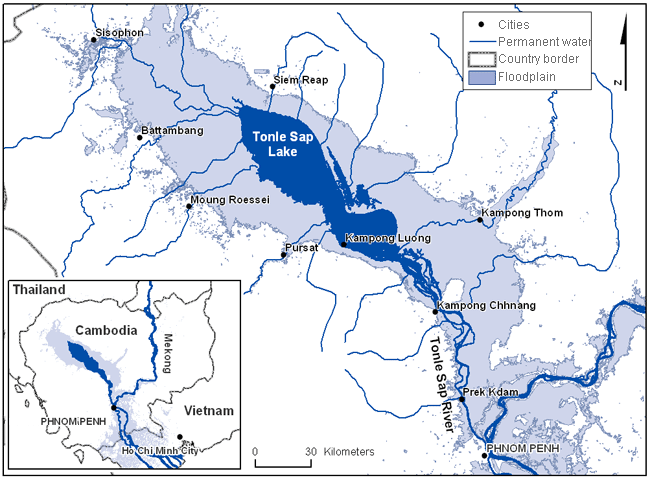
\includegraphics[width=\linewidth]{images/floodpulse/TonleSapMap}
\caption{Map of Tonle Sap (Source: Wikicommons}
\label{fig:tonlesap}
\end{figure}

Throughout the year, the Mekong River experiences significant flow alterations due to the seasonal monsoon (FIND SOURCE). Because of this, the water level in the Tonle Sap is controlled by the water level in the Mekong main stem.

Because of the unique weather patterns of southeast Asia and connection between the Mekong and Tonle Sap, a unique flood pulse system is created. The flood usually lasts an average of 258 days, or 71\% of the year. On average, the flood begins at the end of June, peaks at the beginning of October, and ends in early March, with some variation of course. During the wet season, the Tonle Sap's size expands by about four or five times, and this water then flows into the Mekong during the dry season as its level drops (Evans et al. 2004). This creates a distinctive flow pattern, in which the river's main stem actually flows in opposing directions in the flood season and dry season (SOURCE).

The Tonle Sap ecosystem is also one of the most heavily relied-upon ecosystems in the world. The lake is especially important to those in Cambodia and the lower Mekong Basin; in this area, over one million people depend on the natural resources of the lake . In many areas of the basin, water resources are used intensively at a small-scale loval level. However, the Mekong basin is under rapid development, including the construction of large-scale hydropower dams, deforestation, development, and climate change . However, recent research has found that the construction of dams and other development activities may significantly alter the hydrology, and therefore the health, of the ecosystem.

\section{What is the Flood Pulse System?}

Scientists who study riverive systems, such as water flow, channel morphology dynamics, and plant and animal organisms have tried to characterize streams to better understand them and make predictions about them. 

The Flood-Pulse Concept does exactly this. By acknowledging how rivers can extend well beyond their low flow channels and flood a broad lowlying area on a seasonal basis is a clear pattern of certain rivers, especially those that experience highly seasonal rainfall that is a characteristic of monsoon climates.

\begin{figure}
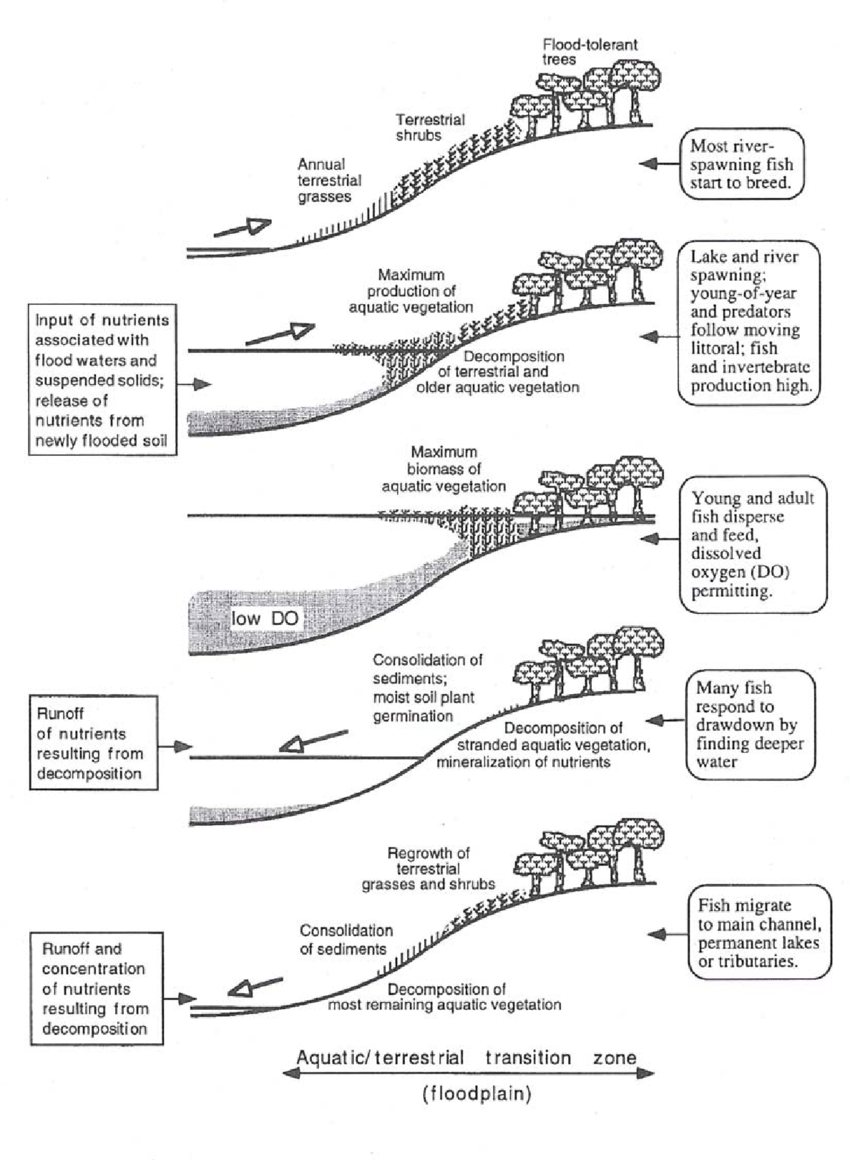
\includegraphics[width=\linewidth]{images/floodpulse/flood-pulse-concept-of-Bayley-1995.png}
\end{figure}

\subsection{Habitats in the Flood-Pulse System}

The floodplain vegetation is one of the most important elements of the Tonle Sap ecosystem. Because  they are inseparable in terms of water, sediment, and shared organic material, rivers and their respective floodplains are considered the same unit, and they work as a combined river-floodplain system. Floodplains are defined ecologically as areas that are periodically inundated by the lateral overflow of rivers or lakes, and/or by direct precipitation or groundwater (The flood pulse concept in river flood-pulse systems).  The river-floodplain system comprises a permanent moving-water ecosystem (lotic), a permanent marshy, stillwater habitat (lentic), and the floodplain. Despite many researchers’ efforts, it is impossible to apply stable and defined borders between land and water in any floodplain.

\subsection{Organisms}
This p  eriodic flooding produces similar anatomical and physiological adaptations in the organisms inhabiting different areas affected by the same phenomenon, and it produces characteristic community structures. The life cycles of organisms in the floodplain are very related to the timing, duration, and rate of rise and fall of the flood pulse system. As an ecosystem, floodplains are very unique because they have both aquatic and terrestrial phases. This leads to specific adaptations among both aquatic and terrestrial animals. For example, aquatic organisms are selected to populate the floodplain at rising and high levels because of the abundance of food. Conversely, terrestrial organisms have adapted to take advantage of the floodplain at low water levels.

\subsection{Nutrient Patterns}
The  lateral exchange of nutrients between floodplain and river channel has the most direct impact on the biota of the ecosystem. The floodplains receive all nutrients directly from the main channel; however, because of their differing biogeochemical cycles to the Mekong River and Tonle Sap, the floodplains develop a different nutrient profile (The flood pulse concept in river flood-pulse systems). These nutrients include both organic and inorganic compounds, that can be further divided up into gaseous compounds, dissolved solids, and particulate matter.

\subsection{Hydrology}

\subsubsection{Climate, Monsoons, and the Holocene}

@article{penny2006holocene,
  title={The Holocene history and development of the Tonle Sap, Cambodia},
  author={Penny, Dan},
  journal={Quaternary Science Reviews},
  volume={25},
  number={3-4},
  pages={310--322},
  year={2006},
  publisher={Elsevier}
}

\subsubsection{Ecosystem Productivity}

The Tonle Sap ecosystem is widely perceived as an ecosystem with naturally high productivity. The Asian Development Bank even considers the productivity of the lake to be ``among the highest in the world'', and this is widely believed to be because of the flood pulse system itself. However, most of the beliefs surrounding the ecosystem productivity of the Tonle Sap actually refer to fisheries production and productivity. Despite fish catch statistics being incomplete and historically unreliable, there has been no research or specific data collected to determine either the primary or secondary productivity of the ecosystem.

Therefore, fish catch data must be used as an indication of ecosystem productivity in this situation. Another powerful indication of the ecosystem's productivity is the livelihoods that are supported, either directly or indirectly, completely or partially, by the river-lake system.

Because the surrounding communities and other users of the lake’s natural resources are especially dependent on its productivity, the lake's ability to support these communities’ livelihoods is a robust way of determining its productive capacity. This also makes the ecosystem's productivity especially important, in that it is not only a key factor of environmental health, but it is also a key determining factor for social equity and economic welfare.

Ask: what is the best way to talk about fish catch data? It seems very all over the place from family fisheries to large scale operations. Would a description/summarization of the data be helpful, or should I just summarize overall findings and trends?

\section{People and the Flood Pulse System}

\subsection{Anthropology}
	The Tonle Sap's abundance of fish and sustenance has been documented for centuries. It has even been hypothesized that the Tonle Sap's productivity was the basis for the development of the Khmer Empire: The huge productivity of the Tonle Sap sustained a Khmer empire at Angkor from 802 C.E. until the fifteenth century. (Evanssourcefromthissource) 

\subsection{Human Impacts on the Flood Pulse System}

\subsubsection{Hydropower Development}

\subsubsection{Climate Change}

\subsubsection{Urbanization and Development}

Main focuses:
•	Importance of flood patterns
o	Not just a diagram, but also math about how floods are measured/work
o	Some equations/acknowledgement of hydrology that looks at flood patterns and that can also tie in with the climate change section
•	Define lentic and lotic
o	Identify groups of organisms that like the different types of organisms
o	Then we can link that in the productivity section
o	Look at California levee that broke and filled in farmland and the fish were more successful in the flooded zone
o	Carbon input and insects in floodplains look at carbon input in lotic zone and lentic as well
•	River continuum concept
o	Historical development, the flood pulse system was in response to the river continuum concept
o	Ignores the lateral movement of  water
o	This will be helpful in the lotic zone of the river
o	Only covers part of the reality
o	Flood pulse model only covers part of the reality too. So we need to put them together!!
•	Use case studies of specific fish to explain the larger processes going on in the river
o	Can even use case studies from north America and Europe and hypothesize about what could be parallel in the Mekong
•	Don’t pretend like you know all the answers, invite questions, and POSE questions
•	Ecosystem Productivity: tell the reader how fisheries are measured and WHY that’s uncertain
o	Also define primary productivity and secondary productivity and how that’s measured in real life, like how do scientists figure that out
•	Look up river culture: an eco-social approach
•	Values of inland fisheries in the Mekong river basin
•	Influence of built structures on the tonle sap ecosystem
•	Civil society and interdependencies chapter on the tonle sap
•	Ngo doing toilets on the lake, what local ngos are doing
•	Look at Lucas’ article “Design With Nature” for inspiration
•	Should I include the Delta in Vietnam?? Food for thought
•	


Ecosystem Services

Fish stocks

Fisheries

Immigration and emigration


\chapter{Hydroelectric Dams in East Asia}

\chapterauthor{Quyen Hoang Ballagh}

\section{Former Residents of Balui}
\red{if you have subsections, try to include one after the section to keep the hierarchy consistent}

Prior to construction of the Bakun Dam, dozens of different Indigenous communities practiced subsistence farming, hunting, and rich cultural traditions along the Balui River. Indigenous communities such as the Kayan have developed and practiced knowledge of the environmental (Traditional Ecological Knowledge) for centuries in agriculture such as rice cultivation. Traditinoal tattoos, stretched earlobes, and connected apartments known as long houses have been the practice of communities such as the Kayan and others who live[d] along the Balui River until development of a megadam called the Bakun Dam which disrupted their watershed and displaced thousands of communities members from their homes \citep{aiken2015dams}. A series of case studies was conducted with the community forcibly displaced to government-controlled Sungai Asap in September 2002. The following quotes are pulled from anonymously interviewed Indigenous village members on comparing the conditions of their original home and their government controlled resettlement in Sungai Asap \citep{choy2004sustainable}. They are translated to English as directly as is possible. \blue{great start}

\subsection{On Survival}

\red{subsections create numbers, do you just want to give the quote some framing? we could try using a minibox or just a bolded text?. if you want to use subsection without the numbers, we could do subsection*}
\begin{quote}
``Life has been difficult for us since we moved to this area a few years ago. Now we are running out of means to buy our foodstuffs to pay our water and electricity bills. You just look at the electricity meters up there, supplies have been cut off as we have not been able to settle our electricity bill for months.'' \emph{}
\end{quote}

\subsection{On Social Change and Economic Development}
\begin{quote}
``I do not think the Bakun project has brought us social and economic development as claimed by the government. The environment here is just not suitable for us. Last time we did not have to worry about our daily consumption because we got everything from the forest. Now everything is so different. No money, no food. Just look at the three acres of farmland allocated to me; it takes me about 20 to 25 minutes by land cruiser to get there. Yes, the government built the road for us but where is the means of transport? A return trip from here (Sungai Kojan) to my farmland in Sungai Asap cost me RM4 (US \$1.05). That is very costly for me.''
\end{quote}

\blue{long quotes don't need quotation marks}
\subsection{On Returning Home}
\begin{quote}
 [If given the chance, would you return to your original settlement?] 
 
``Of course! [The] former settlement is better. Furthermore, when we are asked to pay for the house installment amounting to RM52,000 (US 13,684), we are ''habits'' [finished]. Where do we have the means to pay? Makan pun susah [Eating is also a problem]. By then, we have no choice but to go back to the jungle.'' 
\end{quote}

\citep{choy2004sustainable}\red{put inside the long quote or as a indented citation?}

e.g. 
\quad \quad \quad \quad\quad\quad\quad\quad --As quoted in \citet{choy2004sustainable}.


\begin{figure}
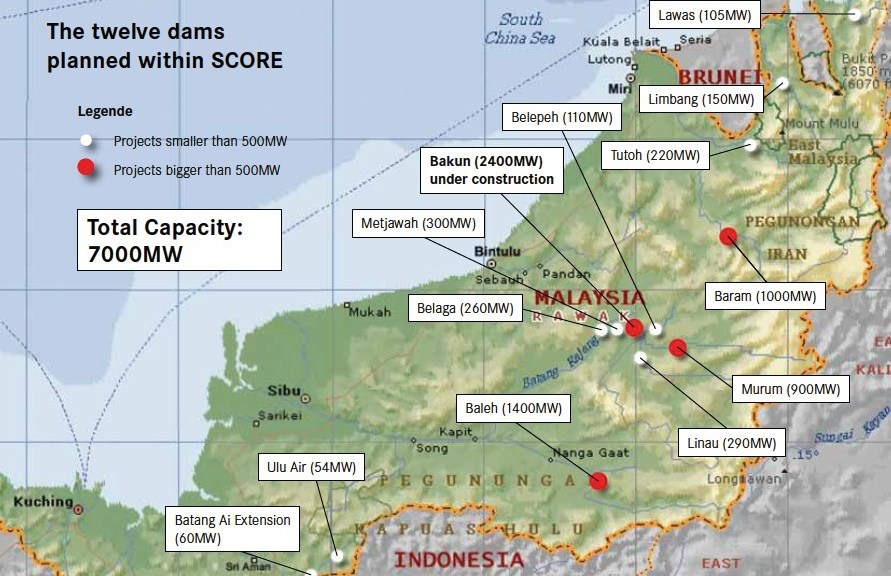
\includegraphics[width=\linewidth]{images/hydroelectric/borneomap.png}
\caption{CAPTION--great figure!}
\label{fig:refborneo}
\end{figure}

\section{Introduction}

Megadams across the globe have \st{caused the }forced displacement of between 40 and 80 million peopled (Hai, 2016). Hydroelectric dams account for 19\% of the world's electricity needs. In Sarawak, Malaysia on the island of Borneo, dozens of new megadam projects are set to be built with plans to account for 7,000 megawatts of electricity by the end of 2020, and up to 20,000 megawatts of electricity on a long-term scale. For reference, China's annual electricity needs are in the 5.8 billion megawatt range and the U.S.was in the 1.2 billion megawatts range in 2020 \citep{gullen2013statista}.\blue{convert to per capita for the comparision?} 
    
  Hydroelectricity and mega dam projects are notorious for displacing billions, disrupting \red{Idd}igenous and traditional modes of livelihood, social structures, and impacting the social-emotional well-being of millions. Additionally, one of the largest ironies of hydroelectricity is \blue{the divergence between who are?} the benefactors and recipients of the produced energy\blue{good addition, but a bit awkward\ldots, fix as you see fit} With the harnessing of hydropower, large construction and deveopment companies profit off of the ecological and humanitarian degradation involved to generate electricity in megadams. Conversely, Indigenous and local populations bear the burden of the development a process termed water grabbing. In most cases (specifically with mega dam construction), the produced electricity is either exported to nearby urban cities, or, in the case of regions like Sarawak, Malaysia, the energy is often exported to different countries altogether. It is estimated\red{passive voice} that in Sarawak, local energy demand in 2020 was about 972 megawatts with estimated increases to 1,500 megawatts annually. Despite the low energy demand in the region, the dams in the area including the Baram and the Bakun both have approximate averages of 1,200 MW (megawatts) of annual production. In most cases, the produced energy (which far exceeds the regional demand) is exported to other regions or countries and the displaced Indigenous groups are not granted access to the energy (\blue{Stephenson}). This is in part due to the funders of dams and who facilitates construction.\red{great transtion, let's see if we can entice the reader with a shorter sentance} Prior to the late 1900s (1940 to roughly 1970-1990), dam construction was funded by the World Bank \citep{awojobi2015were}.
  
      One of the reasons that dams were seen as a critical part of \red{"}development" and subsequently funded by large investment groups such as the World Bank was because at the beginning of the 20th century, the United States and North America began to be used. President Roosevelt of the United States began construction of large dams in the 1930s in the New Deal \citep{billington2006big}. This development continued in post World War II economic and population growth \citep{severnini2014power}. As colonization and imperialism occured in proxy states throughout the later half of the 20th century, countries such as Brazil and China began to encourage hydropower development \citep{folch2019hydropolitics}.\red{red, you can add a line to start a new paragraph}
      
    For example, Brazil during the 1970s under Alfredo Stroessner's dictatorship and U.S. imperialism in Latin America, dam construction was viewed as the pinnacle of modernity and development (in part because dam development was so prominent in the United States in previous centuries) \citep{folch2019hydropolitics}. Under U.S. control of Latin America, the military dictatorships and big loans for development projects from funders such as the World Bank enabled mega\red{did you define mega?} dam construction such as the Itaipu in Brazil which is the \st{next} \blue{second} largest dam \blue{in the world} \st{ to date} after the Three Gorges Dam in China \citep{mainardi2017first}.

   The World Bank began funding projects such as The Three Gorges Dam (one of the largest and most notorious hydroelectric dams) as well as the Sardar Sarovar Dam in India, the Chonoy in Guatemala, and the Itaparica hydropower project in Brazil\red{start with this one since it's from the previous paragraph} as well as countless others. Beginning in the 1970s, criticism arose about the lack of social protection policies for the local and Indigenous communities \st{that} \blue{affected by} dam construction\st{ was impacting} \citep{awojobi2015were}. Action was\red{passive voice} called to both assess, and end the harm caused by the World Bank so the World Commission on Dams was released, outlining the human rights abuses by the World Bank and they withdrew official funding from hydropower projects in the 1990s. Despite this, other corporations have filled the gap in funding, namely actors based in China such as the China Three Gorges Corporation and Sinohydro \citep{cooke2017limits}. 
  
Since the 1990s, alongside a global push for renewable energy sources, construction of hydroelectric dams surged ({See Table~\ref{tbl:bigdams}})--specifically in East Asia with over 10,000 of the dams (approximately 28\% of all worldwide dam construction)\red{I am told editors don't like parathetical statements anymore} centered in Asia. Even within that disproportionate 28\%, a large number of dams lie in Laos which has been devastated by Chinese foreign investment and funders. Many even refer to Laos as the ``Battery of [Southeast]Asia.'' In cases of water grabbing in hydropower in Laos, energy is exported to other countries or urban cities and the Indigenous or local groups who were impacted by dam development are not granted access to the benefits of the dams that uprooted their lives. Many of these corporate projects have failed international guidelines on human rights and Indigenous rights, as well as ecological harms (which are often tied to subsistence and cultural reciprocity)(See Table~\ref{tbl:UNrights}). \\

\begin{table} 

\caption{Selected? UN Indigenous Rights Articles \red{more detail}1 column table to list things CHANGE THIS NAME MAYBE\red{reformatted, better? remove quotes; do we need all of these listed? pretty compelling, but not sure.}} 

\label{tbl:UNrights} 

\begin{tabular}{lp{5.5in}}\hline 

Article & \\ \hline\hline 


Article 3 & ``Indigenous peoples have the right to send determination'' \\ 

\rule{0pt}{3ex}

Article 4 &``Indigenous peoples, in excercising their right to self-determination, have the right to autonomy 
or self-government''\\
\rule{0pt}{3ex}
Article 5 & ``Indigenous peoples have the right to maintain and strengthen their distinct political, legal, economic, social and cultural institutions, while retaining their right to participate fully, if they so choose, in the political, economic, social and cultural life of the State.''\\

\rule{0pt}{3ex}
 Article 7 & ``Indigenous peoples have the collective right to live in freedom, peace and security as distinct
 peoples and shall not be subjected to any act of genocide or any other act of violence, including forcibly removing children of the group to another group.''\\ 
\rule{0pt}{3ex}

Article 8 &  ``1. Indigenous peoples and individuals have the right not to be subjected to forced assimilationor destruction of their culture. 

2. States shall provide effective mechanisms for prevention of, and redress for:

(a) Any action which has the aim or effect of depriving them of their integrity as distinct peoples,
or of their cultural values or ethnic identities; 

(b) Any action which has the aim or effect of dispossessing them of their lands, territories or resources; 

(c) Any form of forced population transfer which has the aim or effect of violating or undermining any of 
their rights; 

(d) Any form of forced assimilation or integration''\\

\rule{0pt}{3ex}
Article 10 & ``Indigenous peoples shall not be forcibly removed from their lands or territories. No relocation shall take place without the free, prior and informed consent of the indigenous peoples concerned and after agreement on just and fair compensation and, where possible, with the option of return.''\\ 


\rule{0pt}{3ex}

Article 11 & ``1. Indigenous peoples have the right to practise and revitalize their cultural traditions and customs. This includes the right to maintain, protect and develop the past, present and future manifestations of their cultures, such as archaeological and historical sites, artefacts, designs, ceremonies, technologies and visual and performing arts and literature.''\\

\rule{0pt}{3ex}

Article 20 & ``1. Indigenous peoples have the right to maintain and develop their political, economic and social systems or institutions, to be secure in the enjoyment of their own means of subsistence and development, and to engage freely in all their traditional and other economic activities.

2. Indigenous peoples deprived of their means of subsistence and development are entitled to just and fair redress. ''\\ 

\rule{0pt}{3ex}

Article 26 & ``1. Indigenous peoples have the right to the lands, territories and resources which they have traditionallyowned, occupied or otherwise used or acquired. 

2. Indigenous peoples have the right to own, use, develop and control the lands, territories and resources that they possess by reason of traditional ownership or other traditional occupation or use, as well as those which they have otherwise acquired. 

3. States shall give legal recognition and protection to these lands, territories and resources. Such recognition shall be conducted with due respect to the customs, traditions and land tenure systems of the indigenous peoples concerned.''\\ 

\rule{0pt}{3ex}

Article 29 & ``1. Indigenous peoples have the right to the conservation and protection of the environment and the productive capacity of their lands or territories and resources. States shall establish and implement assistance programmes for indigenous peoples for such conservation and protection, without discrimination.''\\

\hline 


\end{tabular} 

\end{table}

  In many cases, the current social protection policies that do exist are lacking\red{too vague -- lacking how?} and can lead to justification for displacement. For example, relocation schemes enable hydropower companies to write off the harm they are causing to communities under the guise of some form of [insufficient] reparation. Furthermore, most relocation schemes force Indigenous communities into cramped living conditions with poor sanitation, education, traditional modes of livilihood (including but not limited to subsistence/agriculture), as well as cultural aspects of tradition such as crafts, styles, and familial structure. This, paired with the fact that in most cases of water grabbing in hydropower construction, the Indigenous communities displaced are moved into or not given access to the electricity their lives were destroyed to create\red{need a history of rural electrification}. Instead, many Indigenous groups must find their own way to pay for or generate electricity should they desire it in their community.  


\begin{table} 

%\caption{3 column table example, left justified, right justified, and center justified} 
\caption{These are some of the largest or most famous dams mega dams world wide (energy capacities of more than 400 Megawatts and heights above 15 meters). The Three Gorges Dam is the largest dam globally and produces the most electricity. Dams in East Asia are beginning to be built with more frequency, but other dams such as the Itaipu and Sardar Sarovar are also notorious for their human rights failures. Due to the nature of megadams and the amount of space they need, all of the dams in this chart have caused forced displacement of local or Indigenous populations. TO BE ADDED TO AND EDITTED! \red{I tried to get it to fit!}}
\label{tbl:bigdams} 

\begin{tabular}{llrrrl}\hline 

Dam Name & Location/Watershed & Reservoir Vol. & Height & Energy Capacity & Dam Type \\
        &                    & (km$^3$)      & (m)     & (MW) & \\ 
        
        \hline\hline 

Three Gorges Dam      & China/Yangtze River             & 39.3 & 181 & 101.6x10$^8$ & Gravity Dam\\ \hline 

Bakun Dam & Malaysia/Balui River & 43.8 & 205 & 2,400 & Embankment Dam \\ \hline

Sardar Sarovar Dam & India/Narmada River&5.8 &139 & 1,450 & gravity dam\\ \hline
Son La Dam&Vietnam/Black River &3.1 &138 &2,400 &Gravity Dam\\ \hline
Hoa Binh Dam&Vietnam/Black River& 1.6 &128  &1,920 & Embankment Dam\\ \hline
Nam Ngum & Laos/Nam Ngun River &4.7 & 70 & 865,000 &Gravity Dam\\ \hline
Itaipu Dam & Brazil \& \footnotesize{Paraguay/Parana R.} & 29 & 196  & 96.6 x 10$^8$ & Gravity and Embankment dam\\ \hline

\end{tabular} 
\end{table} 


\section{Dam Function}
  Hydroelectric dams hold water in artificially created bodies of water, or reservoirs. To generate electricity, water is released through a turbine which spins a metal shaft (propeller) within the turbine to convert the energy of the flowing water into energy from movement, or mechanical energy (USGS). Because energy cannot be created or destroyed, the hydroelectric dams convert one form of energy (in this case the energy of the moving water), into another (watts to be distributed to a larger electrical grid for purposes such as energy for a household's lighting) \citep{jansen1983dams}. This type of turbine that turns moving water's energy into electricity is known as a hydraulic turbine (Figure~\ref{fig:USBR})


\begin{figure}
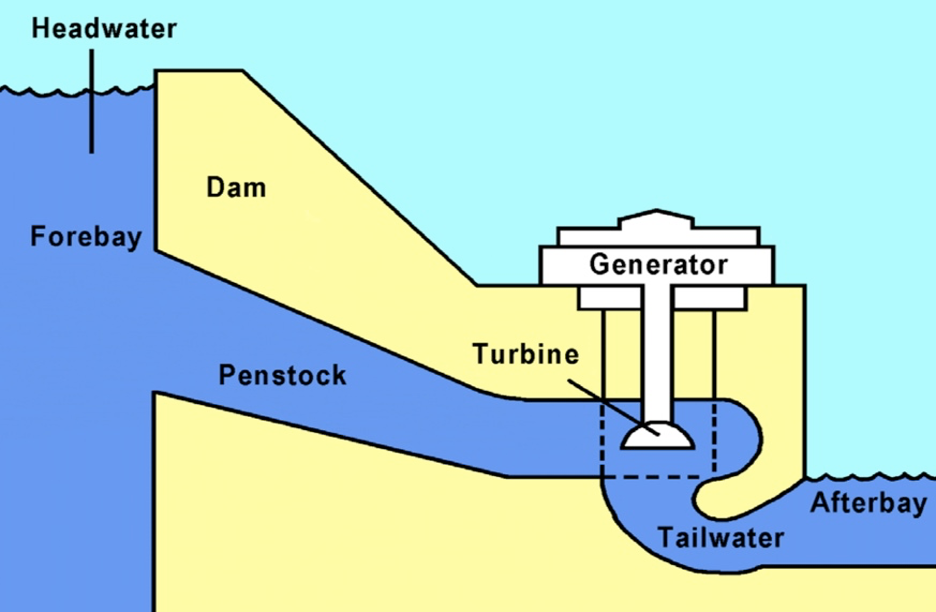
\includegraphics[width=\textwidth]{images/hydroelectric/diagram.png}
\caption{USAGE RIGHTS Available TO ALL/public use The reservoir or body of water is often called the headwater. Water travels down to the forebay, then into a sloped area called the penstock where it reaches the turbine then the tailwater is released into the afterbay (which will be lower than the forebay to allow gravity to move the water to generate electricity for the turbine to collect) (Photo and description courtesy of USBR).}
\label{fig:USBR}
\end{figure}


\subsection{Hydroelectric Generators}

Hydroelectric generators are based on the ideas of Michael Faraday who found that when a magnet moves past materials that allow electricity to flow easily, conductors, the magnet causes electricity to flow through the conductor.\blue{big sentence\ldots, break up a bit?} When direct currents of electricity are circulated through loops of wire around magnetic steel (electromagnets), poles of electromagnetivity are created (field poles).\red{great place for a figure and some discussion of some physics} The field poles are put on the outside of the rotor which is attached to the turbine shaft. When the turned rotates, the field poles move past the conductors and electricity flows, causing an electromotive force, voltage, to develop. 
  
  
\subsection{Dam Type}

\blue{start with an engaging, non-passive voice-- e.g. Dams are not created equally, nor are impact the same\ldots} types vary due to their 
There are \red{passive} differences in artificial dam types that impact structure, function, and energy production. Large dams that are over 15 meters high \blue{mega?} and have energy capacity's of 400 Megawatts or more are termed mega dams\red{okay, here it is, patience, marc}. Two of the most common mega dams are gravity dams, and embankment dams. Another type of dam that is common are run of river dams. Run of river dams can be classified as mega dams or small dams depending on their size. Small dams are also used for hydroelectricity generation although they have less energy production capacity than mega dams.
\red{did you see the talk on dams on Thurs?, I think it was recorded}

\subsubsection{Gravity Dams}

Gravity Dams are dams that are made of concrete or stone and often hollow. They use the horizontal pressure of the water from gravity to create energy. Because they are reliant on gravity, they tend to have large heights and require stable foundations to bear the weight of the reservoirs.
\\If reservoirs are fully filled, the excess water flows over the top in a process called overtopping occurs. Gravity dams are generally resistant to the over-topping flows of the excess water because they are usually made with concrete which is not impacted by the erosion or scouring from the excess water overflow \citep{jansen2012advanced}. Depending on the size of the dam and the required energy production capacity, they can range in height, but in general, higher dams will yield more energy production \citep{lemperiere2017dams}. 

\subsubsection{Embankment Dams}

Embankment dams are usually made from natural minerals such as soil, sand, clay, rock, or occasionally, industrial waste materials. They can also be filled with either compacted earth (hydraulic fill dams) or rocks (rockfill dams) that are smaller than about 3 inches \citep{lemperiere2017dams}. Because of the materials used, embankment dams are generally more susceptible to erosion which means over-topping flows are more of a risk for embankment dams because the excess water can cause erosion of the minerals which puts the dam at risk for collapse or failure because the erosion of the top can cause imbalance of the dam and compromise the structure and the dam could fracture into pieces. Embankment dams are often on some sort of hill or bank with a different levels (high to low elevation) \citep{jansen2012advanced}.

\subsubsection{Run of River Dams}
Run of river dams are usually classified by the fact that the water flow upstream and downstream of the dam is the same\blue{wordy}. Run of river dams should not dam\blue{a bit vague in what you mean} the rivers so drastically to create a reservoir. For this reason, there is \red{passive} a lot of literature that advocates unequivocably for run of river dams as non destructive to the environment. Despite this, run of river dams actually can cause disruptions to fish migration patterns and buildup of soil, rocks, and particles that sink to the bottom of rivers or bodies of water (sediment) around the dam itself in a process known as sedimentation \citep{csiki2010hydraulic}. ADD MORE ON THIS FROM THE ENVIROLABASIA TALK\blue{:-)}

\subsection{Energy}

\subsubsection{Kinetic Energy}

  The size of reservoirs for hydroelectric dams can impact the amount of energy the dam can produce because of the pressure which impacts energy of motion, or kinetic energy. It is the amount of energy from the movement of the water which can be modeled \red{estimated?} with the equation. 
\begin{equation}
KE = 0.5mv%^2%
\end{equation}
In this equation, $m$ is the mass of the object and $v$ is velocity or speed. 

This is important\red{passive} for hydroelectric dams because turbines can be spun through how quickly or strongly water travels in what is termed water flow. The mass of water is 1 kg/liter \red{kg~L$^{-1}$} and the speed depends on multiple factors, including the amount of pressure in the dam. For example, when using a hose to clean dirt from a surface, when the hose is hardly turned on, the flow is weak and slow. The water flow will not clean the surface very well because of the low amounts of moving energy. A hose turned on to its highest setting has larger amounts of water moving through the same sized hose at faster rates. This means the hose would have high amounts of moving energy and clean the dirt more efficiently.
The same applies to hydroelectric dams and how their turbines are propelled to convert the moving energy. The higher speed and pressure means more moving energy which impacts how efficient a dam will be based on size and height. When thinking about a dam with a small reservoir, the amount of water will not create a lot of pressure on the released water, meaning the moving energy is low and the dam will produce fewer amounts of energy. A large dam reservoir will have high amounts of pressure and thus a greater moving or kinetic energy \citep{khawam2006solid}.

\subsubsection{Potential Energy}

Similarly, the height of a dam impacts its energy potential. The higher a dam is, the more the water \red{“}falls” and the higher the potential energy is. Potential energy can be viewed as the amount of energy an object has (or has stored) if moved out of its equilibrium position, so when there is a further height to fall from, the stored or potential energy of the water is greater. This potential energy based on height or gravity can be modeled with the equation:

\begin{equation}
PE_{grav}=m*g*h
\end{equation}

In this, the $PE$ grav is the potential energy, $m$ is the mass, $g$ is the gravitational strength (this is generally based on planet in which it will remain constant at about 9.8N/kg on Earth where N stands for a Newton which is the force needed to accelerate a mass of one kilogram per one meter per second per second), and $h$ is the height\blue{I changed height to h in equation, but make the variable in math mode}. The mass of water is also consistent at 1~kg/liter on Earth. With this in mind, the gravitational potential energy of water (as is the case of hydropower) is based on the variable of height. The higher the dam, the greater the height, and the greater the potential energy \citep{thorin2014basics}.



\subsubsection{Total Mechanical Energy}
There is also a type of energy that is the energy of an object as the result of motion. In essence, it is the stored potential energy and motion energy when moved out of its equilibrium. A simple model for Total Mechanical Energy in dams (assuming there is no bounce of the object [water] in motion), the equation is
\begin{equation}
TME=PE+KE
\end{equation}
In this, TME stands for the Total Mechanical Energy, PE is the potential energy, and KE is the kinetic energy \citep{thorin2014basics}. This means that the most basic way to model the total mechanical energy, or total produced energy, of a hydroelectric dam is dependent primarily on two factors, height of the dam and size of the dam. This is part of the reason that mega dams are favored by development companies—they have larger reservoirs and greater heights which allows the dams to produce more electricity, and thus garner larger profits, even though mega dams require exponentially larger volumes and surface areas which requires more local communities to be uprooted and increased deforestation and other ecological consequences. 

  \begin{figure}
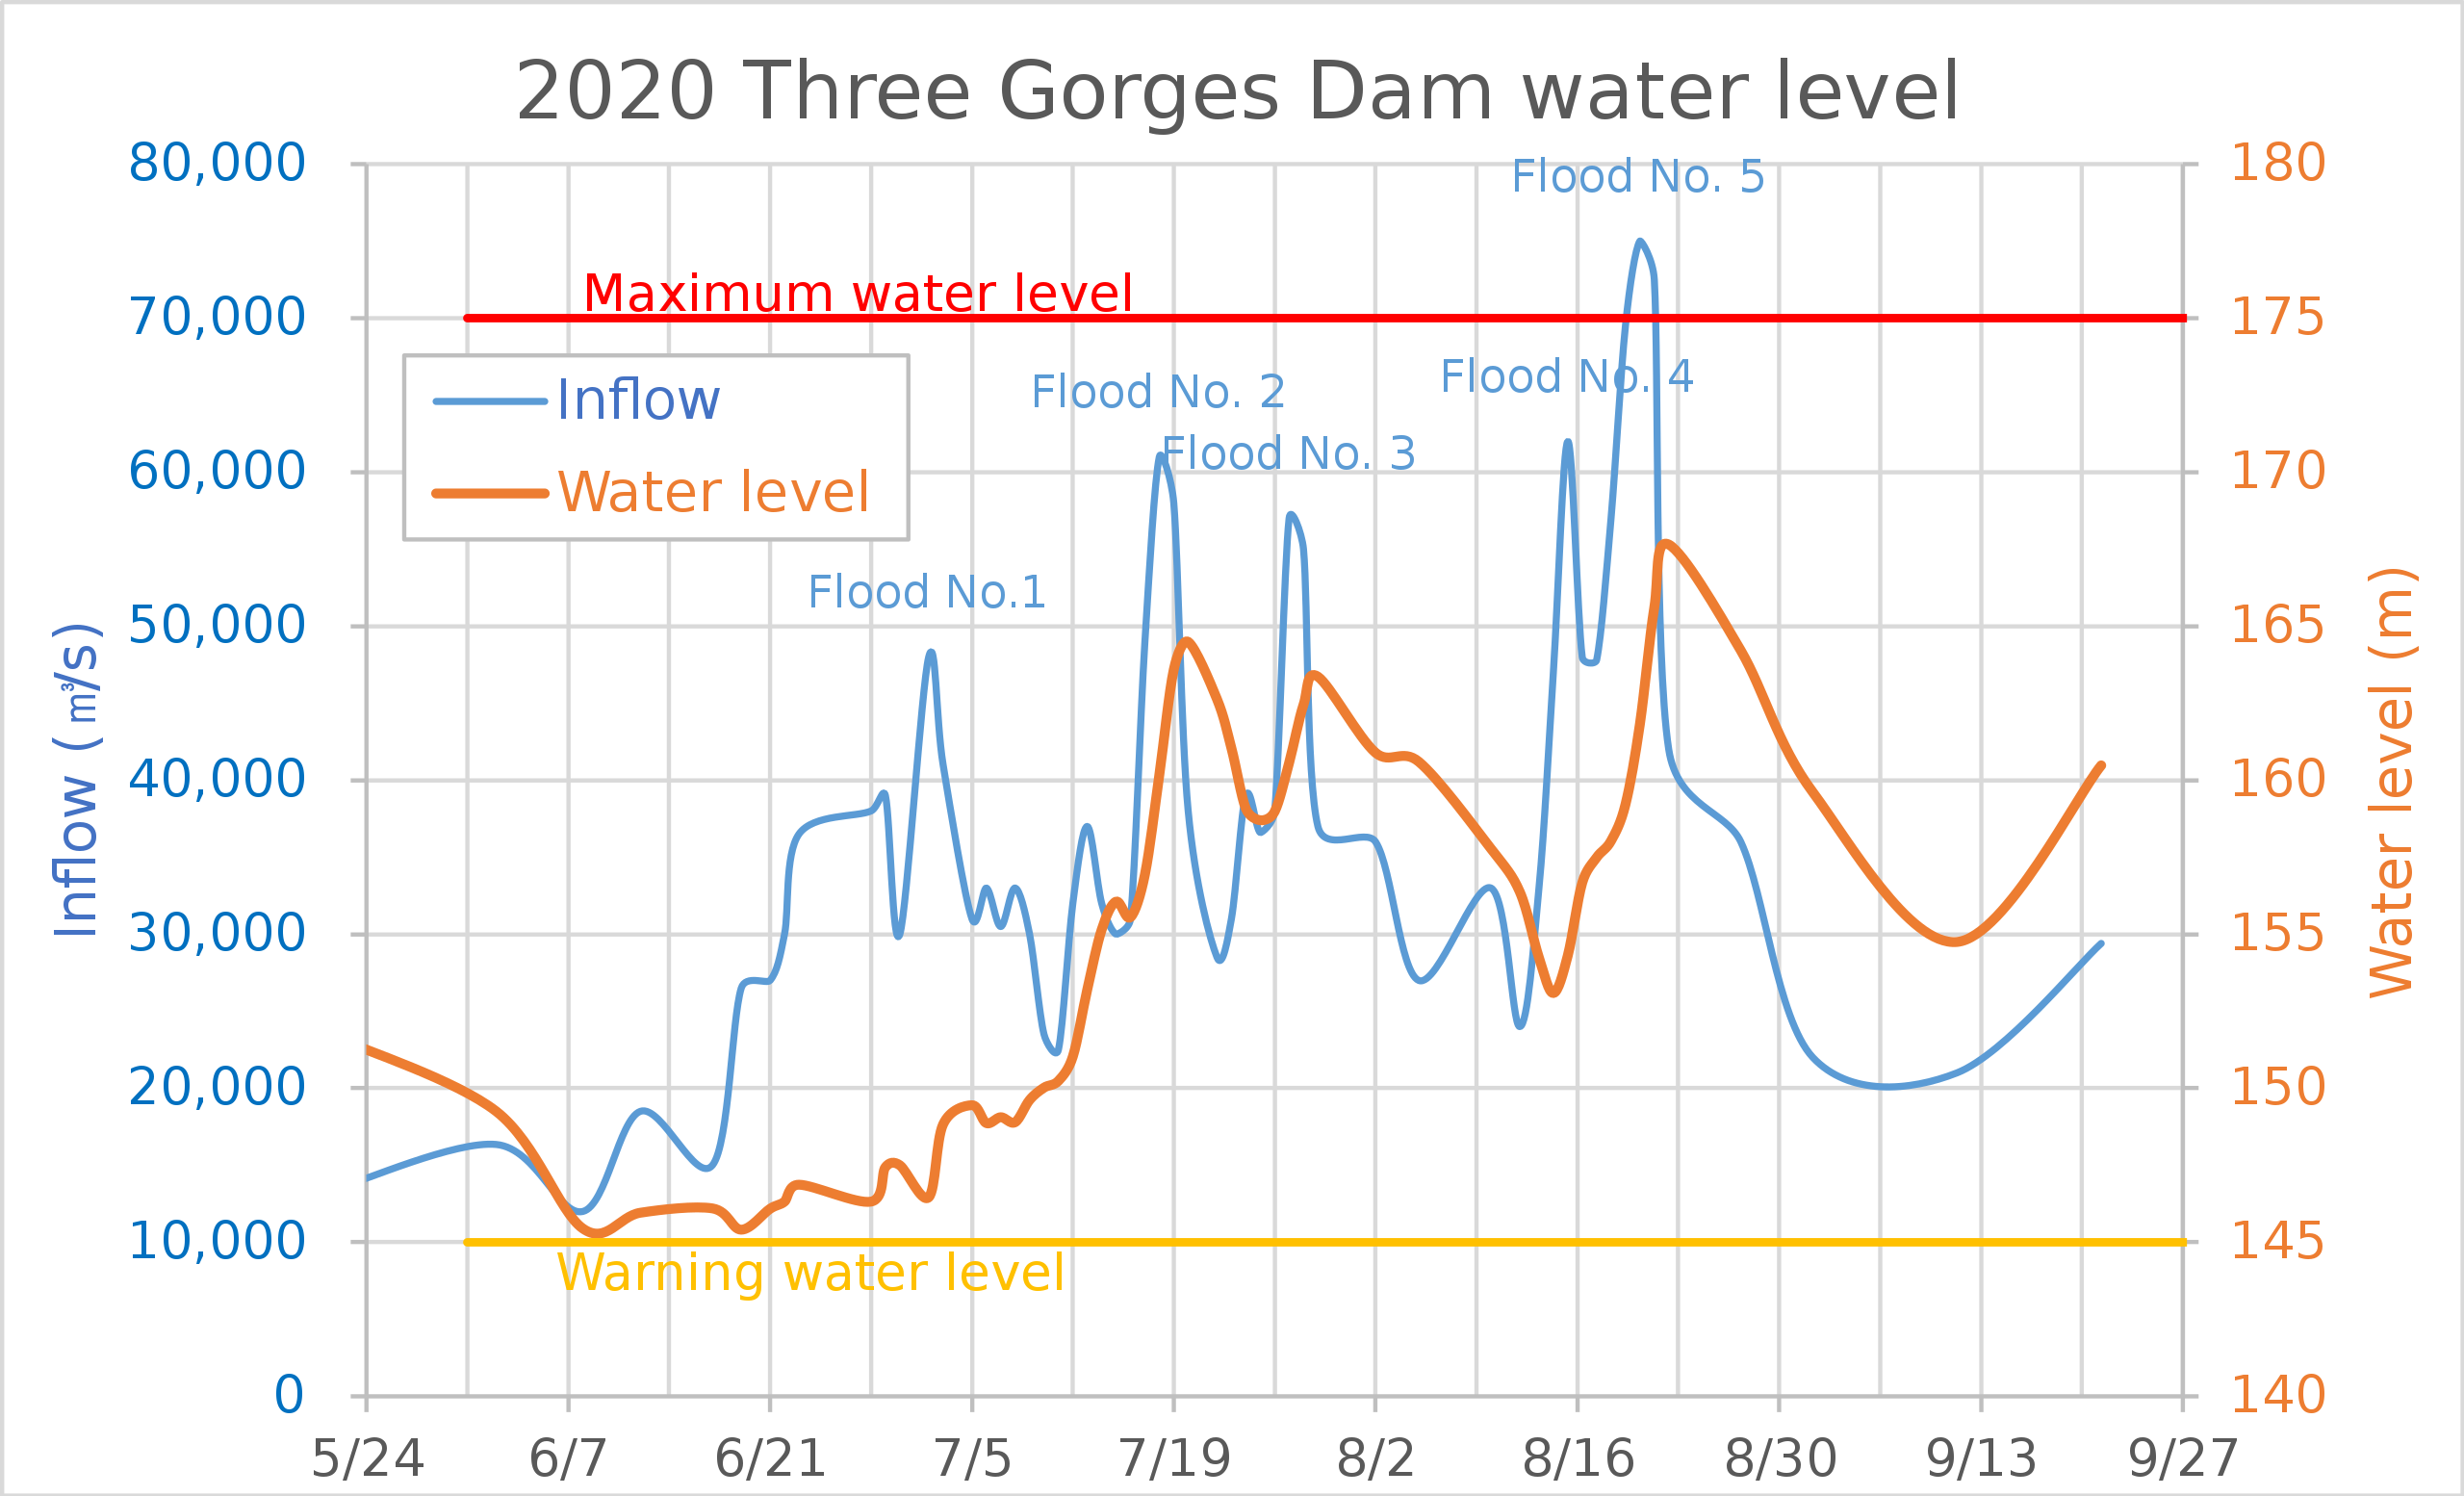
\includegraphics[width=\linewidth]{images/hydroelectric/TGDTME.png}
\caption{This is a graph of the inflow and subsequent water levels of the Three Gorges dam from May to September in 2020. It demonstrates how flooding is both possible and frequent. As the amount of water going into the dam increases dramatically (the inflows), the dam's water levels also increase. This can be seen in each of the floods (for example, flood 2 increased the water levels dramatically on 7/19). }
\label{fig:reftme}
\end{figure}

  
\subsection{Megawatts and Electricity Usage}

   Hydroelectric Dams produce an average of 42 billion kWh (kilowatt-hour) per year. This is enough energy to meet the needs of a developed residential area of about a million people, or 72 million barrels of oil \citep{turner1999realizable} \red{and?} (USBR). To put this into other perspective of just one megawatt is enough energy to power about 10 cars, or 300 homes an hour. Furthermore, part of the reason hydroelectric dams is touted as so efficient is because unlike alternate sustainable energy sources such as solar or wind, hydropower can run at all hours of the day regardless of weather conditions \citep{butler2009headwinds}.
   
\red{Okay, I hate adding to this, but after the talk last week I realized we have another driver -- electrical demand in the region is SUPER high and growing fast. ADDED to that we need to meet that demand without burning fossil fuels. Are we left with hydroelectric or nuclear?  To many yes. That is something we need to engage, I am thinking}


\section{Three Gorges Dam}

  Construction of one of the biggest hydroelectric dams, the Three Gorges Dam in the Yichang Hubei Province in China began in 1994 with the aim to prevent flooding, generate electricity, and to allow ocean freighter ship to navigate inland from Shanghai along the Yangtze river basin \citep{jackson2000resettlement}. The Dam is estimated\ref{passive voice} to have production capacity of 18,600--22,800 Megawatts of hydro powered electricity which accounts for about 10\% of all of China's energy production \citep{xu2011impacts}.\blue{nicely done.}

  By 2012, the dam's 32 turbine generators were all operational \citep{fu2010three}. The dam\red{’}s reservoir holds 5.85 trillion gallons of water and is estimated by the dam’s beneficiaries to eliminate flood related damage for up to a century to protect human development on the banks of a river, or a riparian ecosystem. The dam produces about 84.\red{68 is this important} billion kWh of non-fossil fuel energy a year \citep{wang2003three}. The water flow on the Yangtze has also deepened by the dam to allow ships to carry commercial goods to and from Shanghai to reduce shipping costs by 35-37\% and thus increase profits for large commercial enterprises \citep{wang2003three}.
The number of people displaced and affected by Three Gorges Dam is highly controversial, with estimates below one million (from the Dam's developers) to 10.2 million people in 1996 \citep{jackson2000resettlement}, and estimates ranging up to 900 million people affected (not displaced) due to disruptions in watersheds upstream or downstream of the dam \citep{kittinger2009toward}. 

\begin{figure}
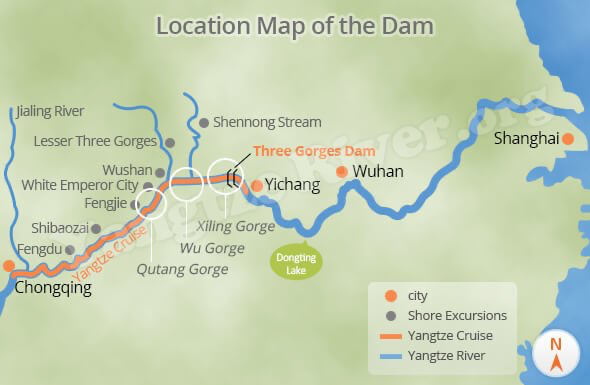
\includegraphics[width=\textwidth]{images/tgd.png}
\caption{USAGE RIGHTS Available TO ALL/public use\\This is a map of the impacted towns along the Yangtze River that the Three Gorges Dam flooded or impacted. Chongqing is an urban center that many displaced populations are forced to move to (it is upstream and was not flooded).}
\label{fig:tgdref}
\end{figure}

  The local region and population around the dam prior to construction was below the poverty line and reliant on agriculture with dense but patchily populated areas \citep{kittinger2009toward}. Literacy rates were lower than the national average and upon construction of the dam, new townships were created to house the local displaced populations, but many displaced people were forced into urban centers for which they were poorly equipped to find work given their reliance on subsistence farming previously\blue{long sentance} Displaced populations were often forced into facotry and production jobs (often for foreign export items) \citep{cernea1997risks} and \citep{cernea2004impoverishment}. 30,000 hectares of farmland that local populations once relied on were flooded and water borne illnesses such as schistosomiasis and other diseases such as tuberculosis and pneumonia become more common in relocation areas due to reduced access to sanitation \citep{cernea2004impoverishment}.\blue{another long sentance} 
  
  Furthermore, psychosocial impacts on the displaced populations were devastating. The complete forced shift away from traditional livelihoods as well as loss of cultural sites and disintegration of social support networks caused traumatic stress, stigmatization, depression, and inter-community violence as a result of the destruction. The Yangtze (a watershed involved in the dam) is known as the ``sorrow of China'' due to the millions of lives the dam project has destroyed both through forced displacement, and even death due to natural disasters \citep{kittinger2009toward} and \citep{jiang2011larger}.
  
  \subsection{Hazards and Flooding}
  
  Another threat posed\red{threat implies future} by the Three Gorges Dam is the impact it has on natural disasters. Due to alterations in the Yangtze’s hydrological patterns, sedimentation and saltation of the basin is also altered. As populations were forced to move, many of them moved to areas downstream of the Yangtze river into areas that are now considered floodplains due to the altered hydrology \citep{world2000dams}. It was predicted\red{passive} that there would be increased flooding and landslides as a result of the dam construction that has since been confirmed in the 21st century (See Figure~\ref{fig:reftme} of water inflows in 2020).
    
  Following the construction of the Three Gorges Dam in the 1990s, the amount of landslides in the region increased. Of the almost 6,000 kilometers of reservoir shoreline, 5\% of it was considered dangerous and at risk for landslides \citep{wu2005comprehensive}. With forced relocation, many people moved into the high-risk shoreline areas, putting them at huge risk for landslides. The increased risk of the landslides is due to the changed siltation and sedimentation which have the potential for loose rocks and sediment \citep{wei1989investigation}. 
  
  Another risk \blue{posed} by dam construction includes flooding; the alteration of hydrological patterns in the region means that previous flood plains are no longer flooded, and new flood plains are established, sometimes in areas population with humans. Estimates from \citep{jiang2011larger} has documented up to 3,000 people having been killed due to flooding in 1998 as a result of the changed to the Yangtze River Basin due to construction. There also exists the possibility for dam collapse should an earthquake occur, although flooding and landslides are more common \citep{world2000dams}. 

\subsection{Displacement}
    One of the common costs of ``development'' is displacement of local and Indigenous populations—-hydroelectric dams are no different. Due to the fact that flood plains are covered in water, the reservoirs themselves take up large amounts of space (in the case of the Three Gorges Dam, an area of over 400 square miles), and local hydrology is often drastically altered as a result of dam construction, forced displacement is a common result of dam building. Displaced has further implications for even more construction and development for the displaced populations\red{—}new infrastructure such as hospitals, schools, roads, water irrigation, and electricity needs to be set up for displaced populations. Unfortunately, new infrastructure for forcibly displaced peoples often is insufficient or inadequate to sustain populations \citep{world2000dams}.
  
  One measurement of human well-being following construction of the Three Gorges Dam was done by \citep{fekete2010millennium} by the Millenium Ecosystem Assessment and World Resources Institute. They classify human well-being under five categories: 
\begin{enumerate}
  \item ``access to basic materials''
  \item ``freedom and choice, health''
  \item ``social relations and social capital''
  \item `` security''\red{don't need quotes}
\end{enumerate}

Due to a number of factors, the MA assessment concluded that the Three Gorges Dam does not meet the requirements to be socially responsible and equitable. \red{can we rank numerous project on this scale to show some variance?}
  
  \red{need a transition :-)}

\subsection{Schistosomiasis}

Snail fever, or schistosomiasis is a disease from parasitic worms called schistosomes. Schistosomiasis causes abdominal pain, diarrhea, bloody stool, or blood in urine. Schistosomes typically live in freshwater snails which are vectors of the disease. The parasite comes out of the snail in freshwater and humans can become infected from skin contact with the contaminated freshwater \citep{verjee2019schistosomiasis}. Snails infected with schistosomes live in freshwater dams such as the Three Gorges Dam \citep{zhu2008three}. 
  
Schistosomiasis is found only in certain areas, making the virus endemic, but along with the construction of hydroelectric dams, snails commonly become vectors for the disease, and they bring Schistosomiasis from the endemic regions. The dams have the potential to increase the quantities of snails entering the region every year, making the disease more common \citep{zhu2008three}. Due to displacement of local populations due to dam construction, this often means influxes of people from schistosomiasis endemic zones enter greater populated areas and this may lead to an increase in infections near the flooded areas.

One of the dams in East Asia that experiences cases of schistosomiasis is the Three Gorges Dam. There is a narrow reservoir attached to the dam that is 1084 \kms which extends into the Jianhan Plain in the Hubei Province and the Chengdu Plains in the Sichuan province\red{—}both regions are endemic for schistosomiasis \citep{zhou2007epidemiology}.
  
  Dam construction throughout the globe such as Egypt, Senegal, and other continents such as South America caused increased cases of Schistosomiasis. African snails for example, have thin and lightweight shells that make their dispersal throughout regions especially effective and dangerous \citep{zhu2008three}. Following construction of the Diama dam in Senegal, a strain of infection from \textit{S. mansoni} snails occurred due to the stabilized water levels. Inadequate health care services in the area of the Diama dam led to an outbreak infection everyone in the city of Richard-Toll (in the dam region) \citep{waldstein1997schistosoma}. 

Despite differences in snail type, the Diama Dam serves as a cautionary tale for large dam construction such as the Three Gorges Dam. Healthcare for displaced populations is limited and due to numerous factors, the Three Gorges dam construction poses increased risk for snail dispersal, breeding, and survival. The most common type of snails in East Asian regions such as the Three Gorges Dam is the \red{O.} \textit{Hupensis} \citep{shi1990schistosoma}. For the purposes of this case study of the Three Gorges Dam and schistosomiasis, the “snails” referred to are of the\red{genus needs to be italized too O. \textit{hupensis} or S. \textit{Japonicum} variety.} 

\citep{nelwan2019schistosomiasis} and the Center for Disease Control observed that schistosomiasis cases occurred frequently in the Three Gorges area after the construction of the dam, with estimates of up to 100,000 cases of infection. If these cases return to their homes from hospitals, the presence of O. \textit{hubensis} in the region could mean their co-existence can lead to increased numbers of infected snails, and later, increased cases in humans. In comparison to other areas of the world, proponents of the Three Gorges Dam argue that there is no correlation between cases of schistosomiasis and the dam, but as evidenced by \citep{zhu2008three} and other authors, The Three Gorges Dam may make the region more susceptible to both O. hubensis (vectors for the disease), and thus increased cases among humans.

\subsubsection{Temperature}

  One factor that has the potential to draw snails to the region of the Three Gorges Dam is the ideal temperature for the snails. The compatible range for the snails was approximately 0.9\degree-21.1\degree C. The Three Gorges region's average temperature is 3.9-18.8\degree C which is not quite currently compatible with that of the snails. Despite this, because the dam has a greater heat capacity than naturally occurring bodies of water in the area, the average temperatures have the potential to increase in a range from 0.3-1.2\degree C depending on the season, making the climate changes more compatible with the snail’s ideal temperatures which may make the region around the dam increasingly ideal for their presence \citep{wenxiang2006index}. 

\subsubsection{Breeding Patterns and Resettlement}

  As displacement of millions of local and Indigenous communities occurred due to the construction of the dam, migrants often resettled as close to their homes as possible away from the reservoir. This means that slopes or hilly areas near the dam are newly inhabited by farmers and the displaced populations, causing soil erosion in the farmed resettled regions, and it causes increased silt deposits in the Hubei region (recall this is a region endemic to the snails). This causes sedimentation and creation of marshlands in areas such as Hubei which are conducive to snail reproduction \citep{jian2000study}.  
  
Figure~\ref{fig:schis}

\begin{figure}
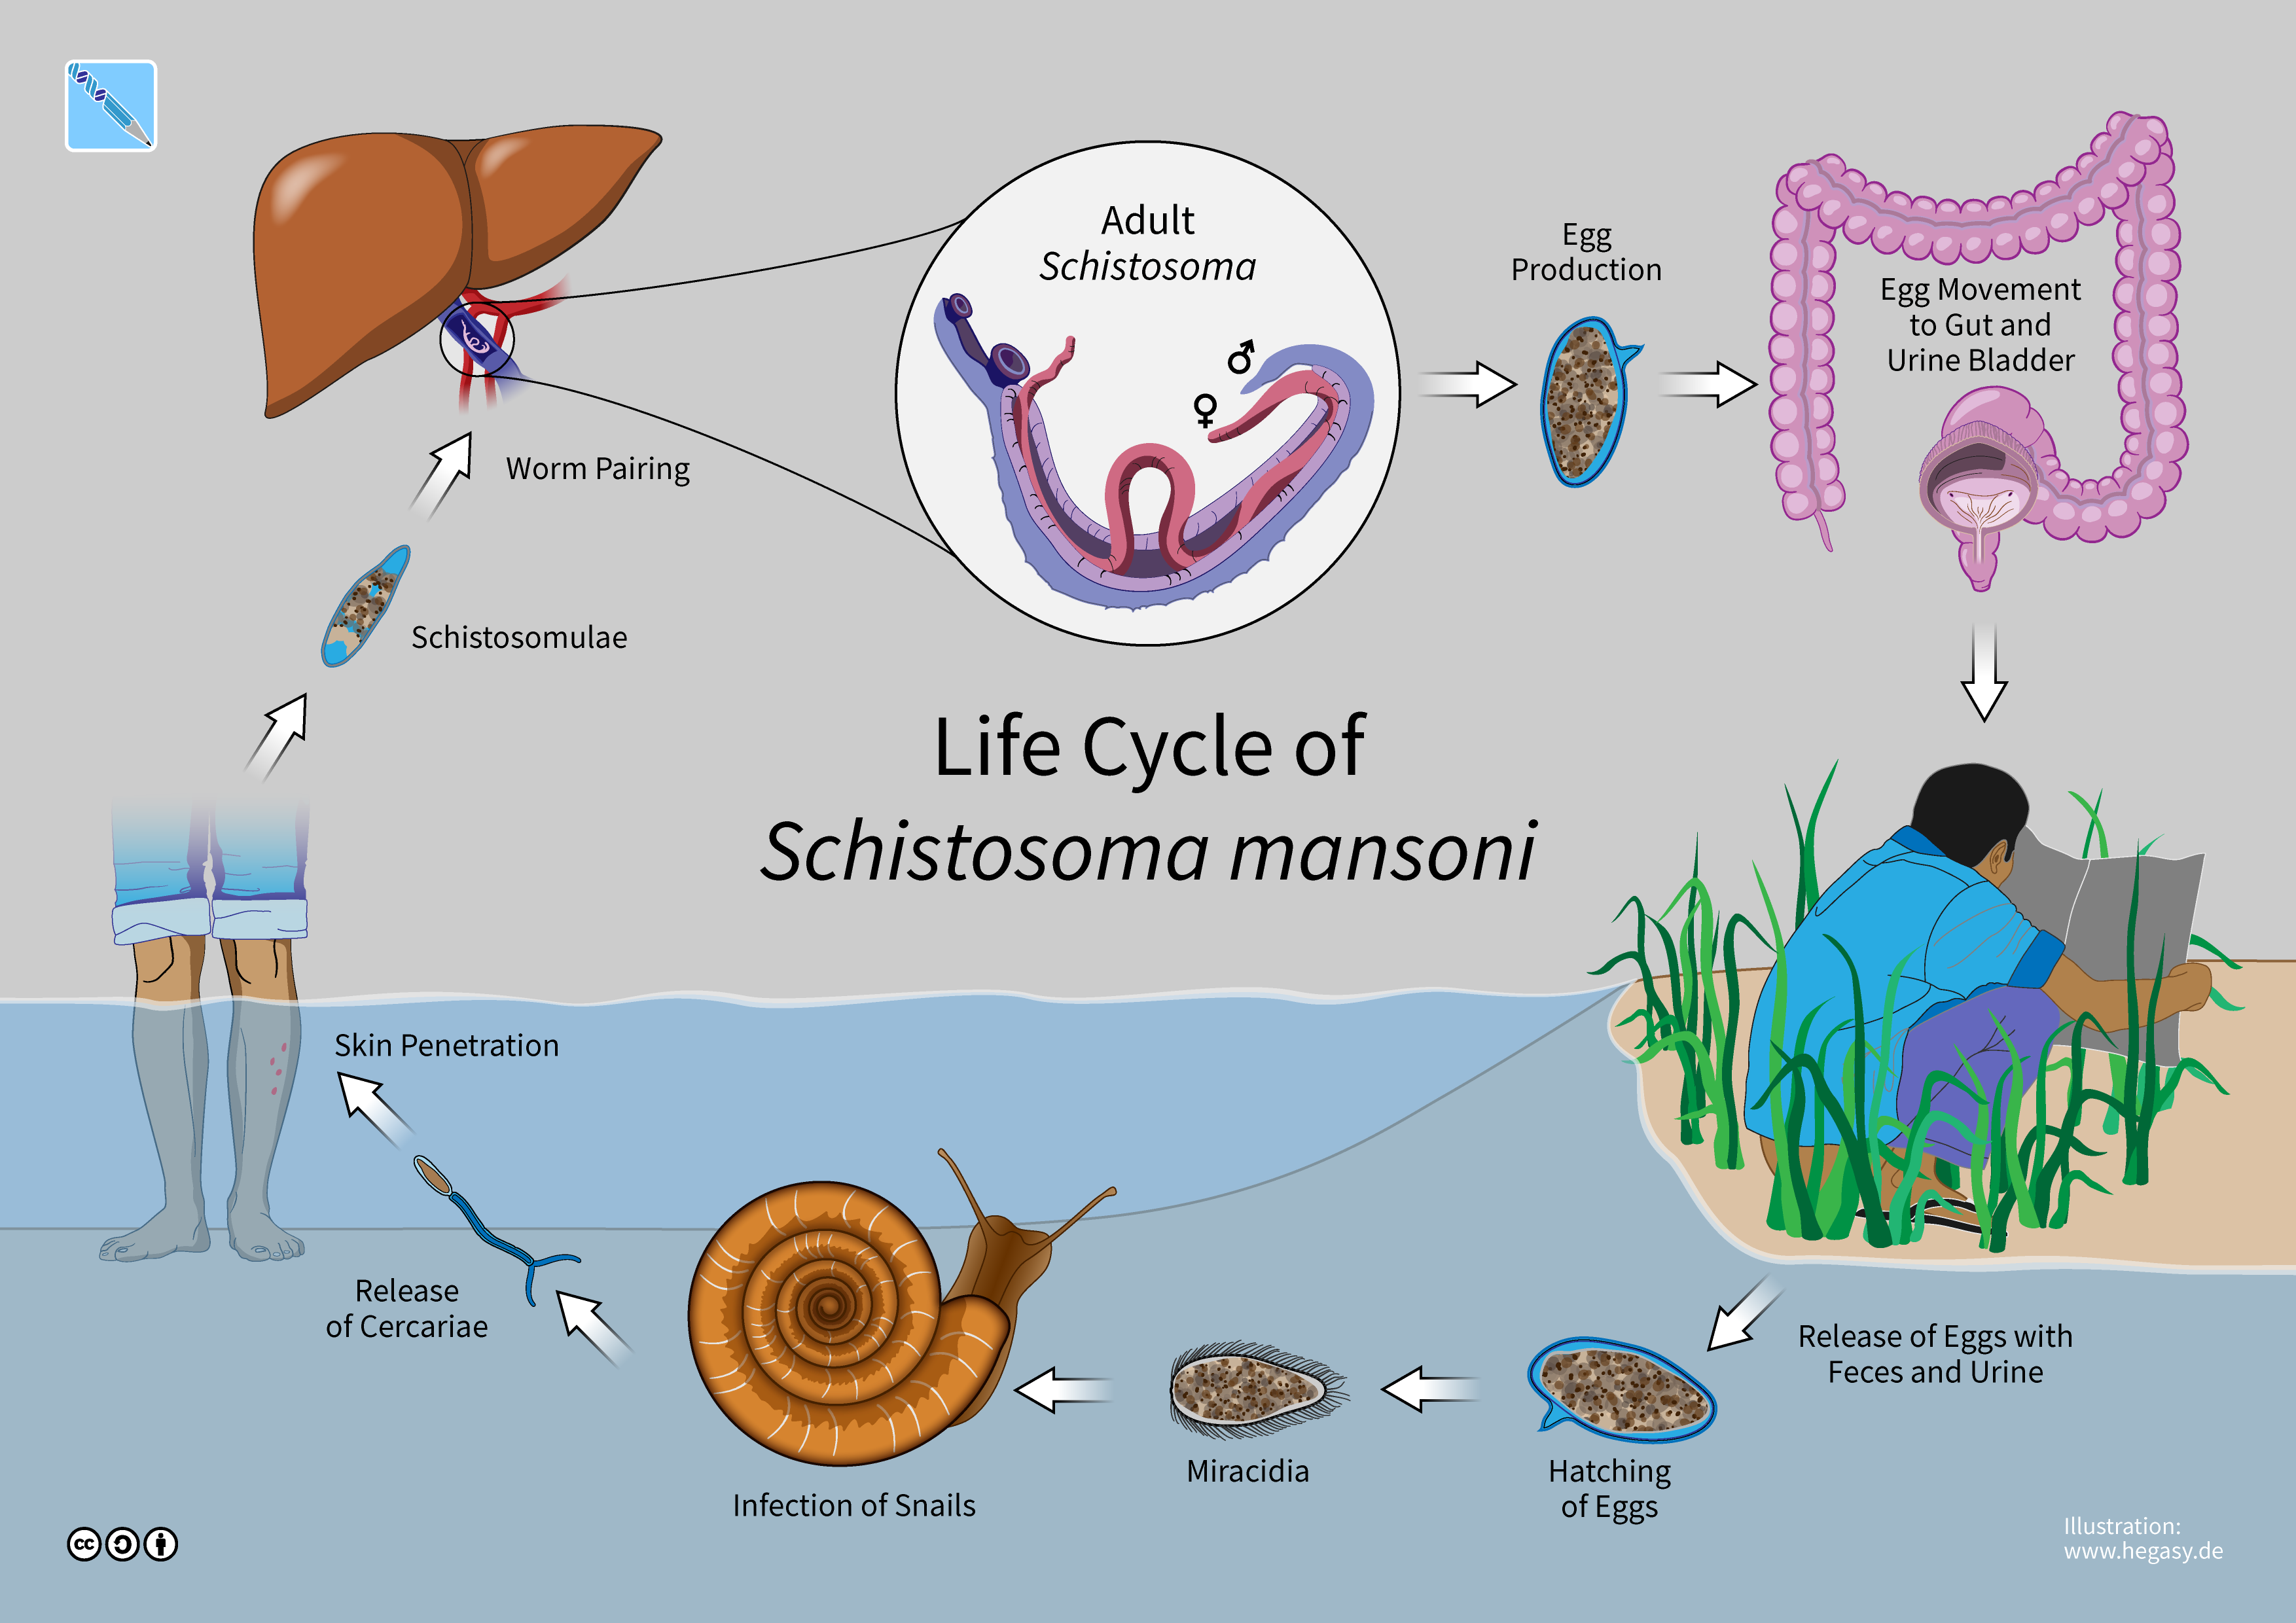
\includegraphics[width=\textwidth]{images/schis-life.png}
\caption{USAGE RIGHTS Available TO ALL/public use. This is an image of the lifecylce of schistosomiasis both inside, and outside of the human body. ADD TO THIS CAPTION}
\label{fig:schis}
\end{figure}

\subsubsection{Snail Dispersal}

  Snails are distributed or dispersed throughout regions in two ways—-actively and passively (Wu 2005). An example of passive dispersal is snails attaching to ships that move to new areas. Active dispersal can look like snails moving across regions via water currents. Passive dispersal does not necessarily have a limit to potential distance traveled, but through active dispersal, \citep{zhu2008three} observed a snail can travel distances of up to 168 kilometers. The closest endemic region to the dam itself is 299 kilometers and there have been documented cases on paper-making reeds that snails and snail eggs have lived on which carried the infected snails across large distances into paper factories in the region \citep{wei1989investigation}. Documented cases such as these imply that the snails could have made their way to the dam from endemic regions through passive dispersal such as the paper-making reeds, or even soil brought into the region that contains snail eggs. \red{citet instead\ldots}\citep{zhu2008three} suggests that the Yangtze River facilitates an increase of merchandise imports which in turn increases the chance for infected snails to enter through passive dispersal. 

\begin{figure}
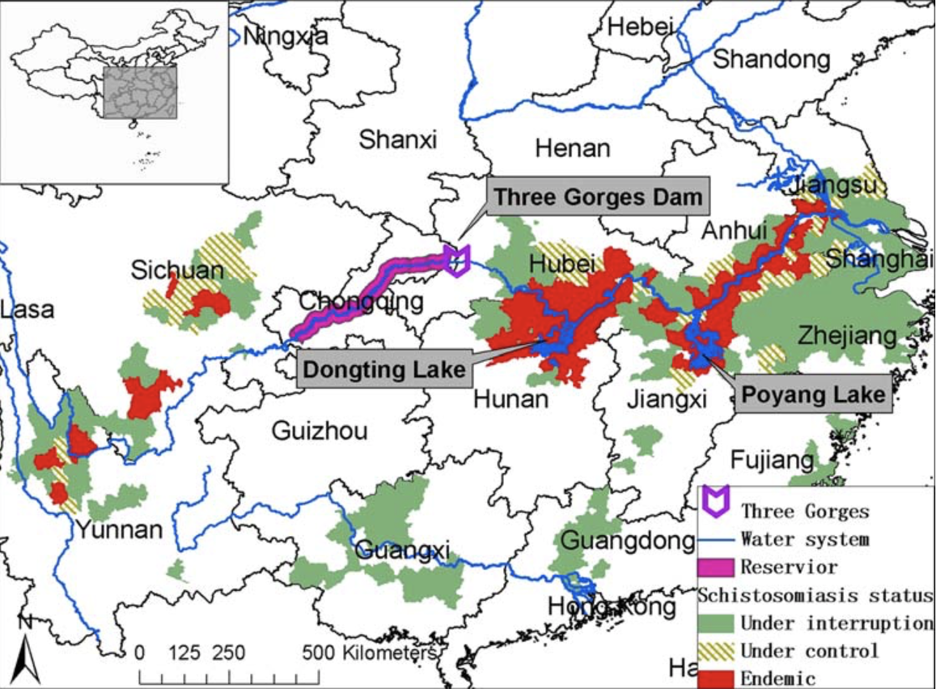
\includegraphics[width=\textwidth]{images/schis-map.png}
\caption{This is a map of schistosomiasis in the Three Gorges Region. As evidenced by the yellow regions, very few amounts of the disease is under control in the region and there is a huge concentration of schistosomiasis just upstream of the dam itself near the flooded regions (i.e., the Dongting and Poyang lake area upstream and east of the dam)}
\label{fig:schis2}
\end{figure}

\subsubsection{Health Infrastructure}

  One of the reasons the risk for Schistosomiasis remains high in the Three Gorges Region is because relocated populations are moved into crowded urban areas which make the possibility for outbreaks and spread of disease higher. Furthermore, insufficient infrastructure (i.e., hospitals, clean water, or proper sanitation) is availbale to prevent or treat the disease. Crowded living arrangements with multiple generations forced into crowded housing also does not aid either sanitation, or the prevention of the spread. For this reason, transmission of diseases such as Schistosomiasis is a threat and danger. Other diseases (water borne or otherwise) are also common, including but not limited to hepatitis, pneumonia, diarrhea, and a virus often spread through rodents—Hantavirus. 

\subsection{Eutrophication}

\red{begin with some discussion of eutrophication defining before jumping into cause, throws the reader (me :-)) off a bit to start about flow changes and toxicity\ldots}

  Outside of Schistosomiasis and the spread of disease, another issue presented by the Three Gorges Dam and other mega dams is altered hydrological flows, increased nutrient sedimentation, and toxin buildup. DISSCUSS EUTROPHICATION HERE

The Three Gorges Reservoir is fed by the Yangtze River (among others). There have been shifts in both water flow, and water levels in the Yangtze as a result and it disrupts the aquatic life, including but not limited to the plankton and microbes of the river \citep{sekiguchi1989case}. An excess of nutrients from runoff leading to dangerously low depleted oxygen levels in the water, a process called eutrophication, has occurred in the Yangtze and its tributaries and watersheds. Agricultural practices that were once not harmful are now causing the eutrophication due to the changed water levels and flows \citep{liu2012effects}.

  Furthermore, industrialization in areas of the Yangtze River watershed has occurred, due in part because of extending urbanization from other areas, as well as urbanization of the displaced populations due to the dam construction.\red{can we map these changes?} For this reason, the nutrient runoff and toxin runoff associated with industrialization and urbanization has worsened \citep{wilmsen2018damming} and \citep{peng2016spatial}. \red{can we show the data?}. Because of the excess of nutrients associated with eutrophication, there have been increased number of scum and deleterious (dangerous) toxins such as neurotoxins which are a threat to public health--this growth as a result of nutrient excess of nutrient loading is known as cyanobacterial algal blooms \citep{fristachi2008occurrence}. This buildup of toxins that effects the water quality is especially prevalent in the Three Gorges region because of the amount of subsistence farming that occurs. 
  
  Most of the local populations in the Three Gorges regions live rural agrarian lives based on subsistence. Populations along the Yangtze River that do rely on the subsistence farming are also hugely dependent on the river for a water source. As the water quality decreases with eutrophication and the buildup of toxins, the local populations that rely on the water and soil nearby are exposed to the toxins that are caused upstream due to industrialization. The water quality can impact crops and nutritional needs, but also daily life water usage such as washing and cleaning \citep{kravitz1999quantitative}.
  
\section{Social Systems and Infrastructure}
  As a result of millions of people being forcibly displaced, local communicties are faced with the question of where to relocate. Some populations move downstream or into regions nearby, maintaining some level of autonomy and subsistence that they had prior to their displacement. Despite having lost often culturally significant lands, this seems to be a better option for many than those who are forced into townships or urban areas such as Chongqing—-an island city at the mouth of the Yangtze in Shanghai that has been growing in population and size where many displaced populations from the Three Gorges Dam were relocated to. (Figure~\ref{fig:tgdref}) In these cases, the displaced populations are forced into areas with existing political institutions which causes social unrest, resentment, and discontent among populations who were once primarily autonomous and maintained soverignty. 
  
  Within these townships and urban centers, there is insufficient living space or housing, education, health care, sanitation, job opportunities, space for subsistence farming/traditional careers, and ironically, energy or electricity. With the loss of 30,000 ha of farming land and government policies to discourage subsistence farming in the region (known as ``de-farming''), malnutrition has increased. Almost half of the resettled populations will not have access or resources to farm and provide subsistence for themselves, driving them away from agrarian jobs into industrial careers \citep{jim2006local}. Forced career changes can be detrimental to mental health and personal/individual agency when stripped of the ability to provide for oneself through traditional modes of subsistence \citep{jackson2000resettlement}. 
  \\    The World Health Organizations reported that similar psychosocial effects are results of displacement such as traumatic stress, depression, and increased violence as a result of the displacement from homelands. Furthermore, social and cultural networks that were once in place in communities collapsed following displacement in many cases. Communities were split up or simply altered so significantly that the social support that was once available has disintegrated. This too causes mental illnesses such as depression. With a lack of health care system for both physical and mental needs, none of the mental health issues are addressed at a health care level. 
\\
       Furthermore, the lack of availability of traditional food sources have led to inadequate diets that have documented cases of having caused chronic diseases and ailments \citep{fekete2010millennium}. It would be naive to group all populations impact by hydroelectric dam construction under the same universal or to assume they all rely on the same modes of livelihood, but a large majority of local or Indigenous populations in dam construction regions rely on agrarian lifestyles. Groups such as the community of Long Lawen and neighboring villages in Malaysian Borneo for example rely on agriculture, hunting, and fishing and this is the case with most other villages in numerous villages in East Asia near dams such as the Three Gorges or Bakun dams.
        A member of the Kayan Indigenous community (former residents of Balui who were forcibly displaced for construction of the Bakun dam) wrote about their subsistence before and after the dam.
    
\begin{quote}
``[Before] the change of lifestyle, we live very close to the jungle and we had a large area where we can hunt, rivers for fishing and we have everything in the jungle, not only food but also medicine. [Now], here [in Sangai Asap] there are 15 longhouses, 10,000 people. There are no rivers where to fish, there is no jungle where to hunt. And even if there were, the little fish or wild animals would end very quickly. Here we have no natural resource. This is the main problem.''
 \emph{Alex}
\end{quote}
        
   Elsewhere, Laos or Lao PDR (known as the ``Battery of Asia'' because of the number of hydroelectric dams in the country), relies on agriculture for up to 80\% of employment and almost a quarter of the country lives at or below the international poverty line \citep{costenbader2015drivers}. Using Laos as an example, the threat to subsistence for forcibly displaced or impacted populations. Rural populations in Laos rely on fish for anywhere between 47-80\% of their protein intake in their daily diets, often supplemented by carbohydrates and fats from other sources including (though not limited to) crops from farming. This means that when displacement occurs, or when watersheds are altered (i.e., flooding to create reservoirs, eutrophication, or other alterations to water quality), so too is subsistence and traditional food sources are disrupted. This often leads to malnutrition and simply insufficient amounts of food. A case study that briefly illustrates this is that of the Ladakh people. Anthropologist and author Helena Norberg-Hodge did a study of the Indigenous Ladakh people and found that with the introduction of dam construction and western development, the Ladakhi’s shifted away from traditional subsistence (both forcibly and willingly). In her time with the Ladakh people, she noticed a shift in diet from the agrarian crops produced, to less nutritious options such as instant noodles which are increasingly popular as an affordable food source for Indigenous populations who no longer have access to farmland or fish. This leads to malnutrition as well as psychosocial impacts from a shift away from traditional nutritious food sources for Indigenous and displaced populations \citep{norberg2000ancient}.

\subsection{Cultural Sites}
  Another issue that is posed\red{create some context first} by the displacement and forced relocation lies in the loss of cultural sites. Estimates of more than 140 villages were destroyed due the dam and it has been impossible to even count the number of cultural sites lost, as well as their value to communities \citep{liu2013chinese} and \citep{du1996university}. This loss of cultural sites such as traditional alters, ancestral lands, or other culturally significant landmarks, topographical features, homes, burial grounds, and other sites lost to the dam construction is incalculable. It is truly impossible to do an accurate cost benefit analysis when comparing the number of megawatts produced as opposed to the unquantifiable number of cultural sites lost and lives altered.\red{agreed, but let's be more sophisticated in how we discuss this -- for example, can you find a source the documents the failure of benefit-costs analyses and cultural values/sites?}
  
  Entire towns and temples have been flooded by singular dam development. The Three Gorges Dam for example submerged the White Crane Ridge\red{—}a hydrology inscription--, the original sites of the Zhangfei Temple--a temple that was removed by archeologists from its original location to prevent it from being completely submerged--, and Dachang—-an ancient town that was submerged and had to be replicated/rebuilt downstream \citep{du1996university}. 

\red{we'll need a transitions and a hint in the intro of the countries you plan to cover}

\section{Vietnam and the Hoa Binh Dam}
\red{create a reason why we want to know about this}
  One of the country's most reliant on hydroelectric energy is Vietnam due to its Riparian ecosystem that makes it ideal for the dams. Between 1995 and 2009, 20 large scale hydropower dams with capacities of more than 100 Megawatts were constructed in Vietnam (Ty, and Westen, 2011). Most of the dams were built in areas populated by ethnic minorities with more than 144 dam investment projects in the Kon Tum and Dak Nong provinces (both rural areas populated with ethnic minorities)\blue{revise to avoid paratheticals} \citep{dao2010dam}. 
  
    \begin{figure}
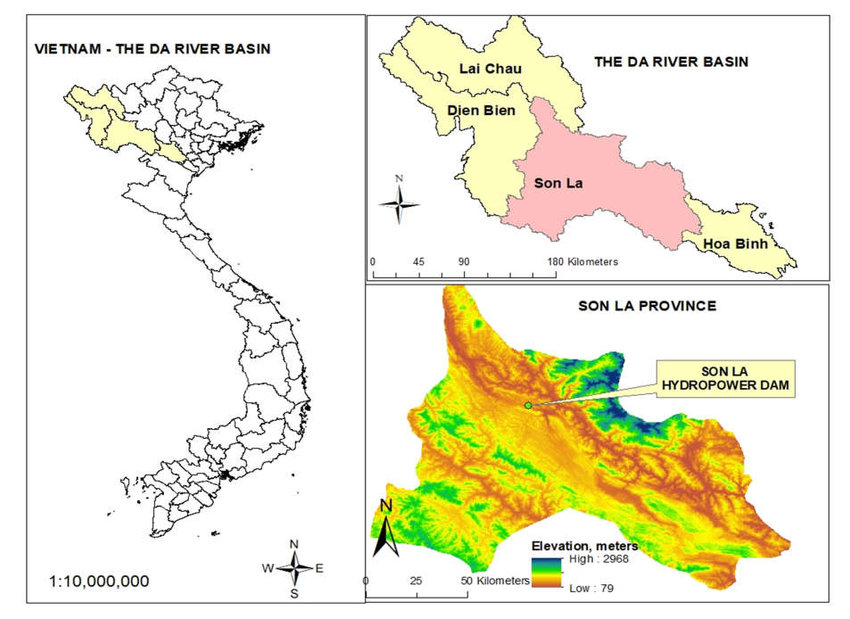
\includegraphics[width=\linewidth]{images/hydroelectric/vietmap.png}
\caption{This is a map of the Da River Basin in the Northwest of Vietnam. Both the Son La and Hoa Binh disrupted the region's watersheds}
\label{fig:refviet}
\end{figure}

  
  Dak Nong for example is located in Vietnam in the central highlands in a mountainous region with generally nutrient rich soils due to high levels of\red{map with soils?} basalt which makes it ideal for farming and many of the people in the Dak Nong province farm coffee, rubber, cashews, sugar cane, and pepper trees. Around 85\% of the population lives in rural areas and it is one of the poorest provinces in Vietnam. Furthermore, the Vietnamese government made it a priority to bring electricity to Indigenous and rural communities in 2004 to reach 100\% of households by 2020 but these goals were not met. Instead, rampant dam construction has occurred at the expense of the Indigenous populations the Vietnamese government tried [and failed] to bring electricity to and they instead ravaged local ecology in the name of progress and energy \citep{thao2019assessment}. \red{again, the history of rural electrification might be good context, many things have been justified by this development goal and the USA is a key part of this}
  
  The dams in this area caused damage to forests and altered river streams and flow speeds, causing sedimentation and erosion which threatened the biodiversity of the rivers and surrounding areas.\red{good, can you give explicit examples?} The 200-kilometer Hoa Binh Dam displaced 58,000 people, 79\% of whom belonged to ethnic minority groups including the Muong, Tay, Dao, Thai Trang and Thai Den \citep{dao2010dam}. The dam destroyed 20,800 hectares of farmland, crop fields, and forests which were crucial to traditional production and subsistence practices of the rural poor in the area \citep{nguyen2013linking}. 
  
  The Muong people for example are the second largest ethnic minority in Vietnam and the largest ethnic minority in the Indochina region. They rely on agrarian farming with crops such as rice. They rely on local resources for subsistence including crops, hunting, and raising animals. They also engage with tourists and western economies to some extent as they gather wood and cinnamon for trade with those outside their communities. The destroyed farmland and crop fields were incredibly destructive for the Muong living in the region impacted by the Hoa Binh dam as it stripped necessary farmland and forests necessary for subsistence as well as products to trade \citep{trang2004local}.
  

  
  Of the 58,000 people displaced by the dam and surrounding destruction to the ecosystem, clean water, education, healthcare, and other basic human needs were unavailable. Up to 34\% of the displaced population did not have access to clean water, and ironically, 20\% of them did not have access to electricity (regardless of the fact that their displacement stemmed from exploitation of their lands to produce electricity for the national grid which they did not have access to). In 2009, poverty rates of the displaced population were 59-60\% compared to the national rate of 14\%.\red{but what were they before?  I can see if they were 80\% for the govn't might call it a success\ldots} Primary school completion was also almost 10\% lower than the national rate.\red{again before?} The Hoa Binh hydropower project demonstrates the lack of comprehensive Environmental Impact Assessments (EIA) and sustainable relocation plans—allowing for the valuation of profit over human life \citep{vinh2014impact}.

\section{Long Lawen and Long Liam}
  Another case study that is important for understanding Indigenous sovereignty alongside the issue of hydroelectric dams is that of Malaysian Borneo, and more specifically, the villages of Long Lawen and Long Liam. Both villages are case studies in which the people protested or refused resettlement and dam construction and they found energy alternatives. This is not to say hydropower development has a \red{“happy ending” }but Long Lawen and Long Liam are arguably more optimistic case studies for the autonomy and advocacy in Indigenous communities.  

  To begin, Long Lawen set some model of an example for what is called micro hydro projects as termed by Headman Gara Jalong of the village. He has been fighting for many years to protect Long Lawen, often at the cost of imprisonment. In the 1990s, the Bakun company tried to forcibly remove the community of Long Lawen to build a mega-hydropower dam called the Bakun Dam. It is one of the largest dams in Southeast Asia to this day in the rainforest in the Belago District in East Malaysia in Sarawak on the Balui river. The village of Long Lawen lives in this area and their original location was in the way of dam construction. The dam is 14,170 \kms (which for reference, is the size of the entire country of Singapore—-this is an extremely large dam). It occupies 12\% of Sarawak and its main funder is a Chinese company. During construction of the dam, the company Bakun was practically uninvolved with the relocation scheme which they left to the local government in Borneo. This relocation scheme required the removal of the Long Lawen village and was intended to remove them to a government-controlled site, stripping them of their cultural autonomy and land.  

  Gara Jalong, as well the community members refused the government's resettlement plan and the community moved independently in a safe area above the dam construction. While an imperfect solution (which already is flawed as Long Lawen should not have been presented with the requirement to move at all), this did allow Long Lawen to remain somewhat autonomous and independent as opposed to moving into the government-controlled resettlement location.
  
  Long Lawen still remains in the rainforest in longhouses with connected apartments for the community members which is the traditional style of residency, and it is not uncommon for the older generation to maintain many of the traditional practices such as stretched long ears, as well as traditional modes of livelihood such as creating forest products and hunting and fishing. Many members of the younger generation prefer western fashion or living. Most of the younger generation moved out of Long Lawen but they still visit annually.  

  In 2000, the Malaysian Senator Banie Lasimbang helped Long-Lawen build a micro-hydro turbine. The science of these micro-dams remains like that of mega-dams (a turbine utilizes gravity to turn and generate electricity), but a key difference is that this micro-hydro power installation was built by, approved by, and desired by the community of Long-Lawen. 

  Through Senator Banie\red{’}s help, Gara Jalong and the community were able to construct a dam that did not displace them or alter their watershed to detrimental effects. One of the \red{largest ironies--better adjective?} of hydroelectric dams as mega projects by outside contractors is that the local and Indigenous communities they displace almost never receive the benefits of the generated electricity. This is the case with Long Lawen which made the micro-dam so appealing to bring “cleaner” and arguably better electricity to the village as it was advocated for by the community members themselves.  

  There are of course limitations\red{passive} to the micro-hydroelectric dams, including but not limited to the amount of energy they produce. For example, during the winter holidays, younger community members and extended family members of the Long Lawen community return home and during this time, the 4-6 kilowatts a day produced by the dam is insufficient for the village. The micro dam was supposed to produce up to 12 kw/day of electricity a day, but the actual numbers have fallen quite short of those estimates.  

  Despite the lower energy production than anticipated, the micro dams have been replicated in almost a dozen other villages in the region including Long Liam who also built a micro dam using Long Lawen as an example. The village of Long Liam also ran into issues with their dam, including technical problems. 
A feature of hydroelectric dams is a penstock which channels the water towards the turbine, but in the case of Long Liam’s micro dam, the pathway towards the penstock isn't a straight path which complicated the efficiency of the energy production. While this is technically fixable, it would require manual labor and be difficult to fix without some level of alteration to the ecosystem (notably though, this alteration would be considerably less than any destruction caused by mega dams, and it would be facilitated by the community members). 

//THIS IS A SUMAMRY OF THE TECH ISSUES COME BACK AND EXPLAIN !\red{sound good!}

  This is not an argument in favor of the mega dams, nor for energy sources such as fossil fuel, just an acknowledgement of the inadequacy of micro dams as a sole energy source for a village.\red{very good, let's talk this week about run of the river dams as alteranatives} Mega dams are so harmful in both the social aspect, as well as the ecological aspect that micro dams may in fact be a potential alternative to the alternative energy source of mega dams. 

  Author of the book Ancient Futures, Helena Norberg-Hodge argues for a transition from globalization and globally based economies/development (such as mega dams), towards localization of agriculture, as well as energy production. She advocates for small-scale energy development projects such as micro dams, but explains that “when it comes to small-scale projects that truly promote self-reliance, such as village-scale hydroelectric installations or solar ovens and water heaters for the household, the question is immediately asked: ‘Can the people pay?’ Nuclear reactors and big dams are heavily subsidized, while small scale-technologies based on renewable energy receive no significant support from any major aid agencies” (Norberg-Hodge 146-147). There is a very fine line to balance between imposition of western technology and aid. Should Indigenous communities or villages desire such village-scale installations of hydroelectric dams (or other energy sources), one must ask whether it is the obligation of global aid organizations to subsidize, or even fully fund such projects. 

  An important part of this desire can be explained by Author John Bodley’s proposal for cultural autonomy for Indigenous nations. He says that its purpose is “establishing the Indigenous peoples’ right to self-determination and ‘helping to secure the future of Indigenous cultures in concurrence with their own efforts and desires: \red{make into enumerated list}
\\1. to focus international attention on the contemporary situation of Indigenous peoples 
\\2. To pressure governments to respect the internationally recognized rights of Indigenous peoples 
\\3. to provide financial assistance to Indigenous peoples in support of their self-determination struggle 
\\which would “permit tribal peoples to choose the degree of isolation they want to maintain (Bodley). These ideas of cultural autonomy for Indigenous community is key in the discussion of both mega and micro hydroelectric dams. Part of the reason most hydropower development so radically violates Indigenous rights is because it ignores land rights and human rights as well as the desires of the Indigenous communities and their right to make decisions for themselves. If village-scale hydropower is an avenue to further explore in terms of electricity generation, it must comply with ideas of cultural autonomy. In other words, any development, even at the micro scale, must permit Indigenous groups to determine the level of involvement and development they would want in their villages.  

\subsection{Conclusion}

  The alternative energy source of mega dams is far from ``clean'' or ``sustainable'' both from an ecological standpoint, as well as from a humanitarian point of view. The water-grabbing that occurs in the mega dam development results in clear winners and losers as big construction companies profit off the ecological degradation and human impact of the dams. The displaced populations face loss of culturally important homelands, as well as threats to social systems and modes of livelihood that are clear violations of cultural autonomy and Indigenous rights. We must halt mega dam construction for good and at least attempt to give back autonomy and agency to the Indigenous groups so deeply impacted. In the face of the Climate Crisis,a departure from this avenue of ``cleaner'' energy production must not occur, but it is key to ensure hydro power projects are smaller, do not cause displacement, and are done at the behest of the local populations they will impact.  




\chapter{The Political Ecology and Economy of Rice in Myanmar}

\chapterauthor{Lucas Florsheim}

\section{Introduction}

As climate change becomes an increasingly concerning threat to agriculture many countries throughout Southeast Asia are rushing to adopt new agricultural practices that subvert issues like flooding and rising temperatures. According to the IPCC, Southeast Asian food production could fall by up to 30\% BY\red{why in caps?} 2050 If certain agricultural adaptations are not implemented (Wassman et al., 2009).\red{let's create the citations using citep{}} Although specific agricultural adaptations and solutions differ depending on climate and region, several scientists have outlined the general changes that will need to be implemented to sustain food production in the face of the climate crisis. \red{is this a new paragraph? add a space to make one}
Adaptive options for confronting issues related to increasing temperatures and hydrological disruption include incorporating crops that are heat-resistant and less vulnerable to salinity stress, improving water management, altering crop management practices, implementing resource-conserving technologies (RCTs), diversifying crops, improving pest management, and creating better weather forecasts and crop insurance (Wassman et al., 2009).\red{wow, this is a mouthful and probably needs to be translated\ldots} While there is \red{passive voice}significant scientific evidence that these methods will indeed work to sustain agricultural production in countries throughout Southeast Asia, many of these adaptations may not be feasible implementations for developing countries with complex political structure and history. 
Myanmar certainly fits the bill of having a convoluted government\red{uniquely or just recently convoluted?} and political history. \red{Did japanese occupation have an impact?} Since its independence from Great Britain in 1948, the country has fallen victim to several coups and has been ruled by its military for most of the last 70 years. Leading up to the Green Revolution in the 19660s\red{:-)}, Myanmar was one of the top rice exporters in the world (Naing et. al, 2008). The deltaic regions of Myanmar had an advantage over other rice producing areas as deep-water or floating rice systems were routinely used the country’s military government was not initially invested in implementing new agricultural methods and thus fell behind other leading rice exporters. Just as lack of infrastructure and varying priorities caused Myanmar to lose its spot as the top rice exporter in the latter half of the 20th century, these factors now actively inhibit the country from performing the necessary implementations in response to the agricultural issues posed by the climate crisis.\red{as a poorer country, how did it fit into the cold war geopolitics?} 
Myanmar has made tremendous progress towards democracy in the last 20 years. This progress culminated in a democratically elected parliament being sworn in 2016, with the elections of 2015 being the first openly contested election since 1990. A democratically elected government is necessary to execute the sweeping agricultural adaptions\red{why?} and to introduce the infrastructure needed to combat the effects of climate change.\red{again, why? Is this always the case?} Earlier this year the military of Myanmar, led by General Min Aung Hlaing declared a national emergency and seized control of the country in a coup d’\red{see how acceants and apostrophes are done in \LaTeX}état. The military is now in sole control of the county’s operations and infrastructure and has spent the last several months attempting to qual both peaceful protests and armed civilian resistance (Goldman, 2021). The overwhelming majority of Burmese people are in \st{absolute}\red{?} opposition to military governance, resulting in daily protests since the coup took place. Since the military seized power on February 1st, over 600 civilians have died at the hands of the government, and thousands more have been injured and arrested (Goldman, 2021).\red{do we want to be more circumspect in case Burmese want to read this?  Could get censured?} 
Combatting the effects of climate change and ensuring food security in Myanmar through sustainable rice production is only possible if the country is politically stable\red{why--I think I agree, but it's important to tell the reader of your assumptions here}. A history of political unrest and conflict inhibiting proper infrastructure and development indicates that Myanmar will struggle to adopt the agricultural adaptations that experts recommend to mitigate the environmental problems of the coming century. \red{new paragraph?}In this chapter we will examine the political economies and ecology of rice in Myanmar throughout history as well as the potential climate related threats to rice production. It is through this analysis that we will attempt to understand the implications of the current state of Myanmar’s government on the future of the country’s rice production in the era of climate change. 

\section{Climate and Rice Production}
Being one of the largest countries in Southeast Asia, Myanmar experiences several different climates, varying greatly based upon region. The most northern parts of the country feature humid sub-tropical climate with hot and humid summers and mild winters. The Northeastern part of the country experiences a temperate oceanic climate meaning warm summers without significant seasonal differences in precipitation. The rain-fed rice producing regions in the South of the country are in either Tropical Savanna or Monsoon climate zones. Tropical Savannah climate classifications are defined by having distinct and differing wet and dry seasons.\red{map of climates?} Monsoon climates are very similar to Tropical Savanna climates, but experience significantly heavier rainfall. Precipitation and minimum and maximum temperatures not only show substantial variation across the country but are also greatly impacted by monsoons. 
\red{I moved your figured to a subdirectory to help organize them.}
\begin{figure}
\includegraphics[width=\linewidth]{images/myanmar/Image1.jpg}
\caption{Average annual precipitation in Asia, the rainfed rice-producing region of Myanmar is circled in red. \red{I wonder if we can find /make a figure for just Myanmar?}}
\end{figure}



\begin{figure}
\includegraphics[width=\linewidth]{images/myanmar/Image2.jpg}
\caption{Climate Classifications of Southeast Asia, with the rice-producing region circled in red. \red{is there a map layer we can use to create maps just of Myanmar?}}
\end{figure}

Temperatures are generally lower in the mountainous regions to the North, whereas the southern portion of the country is much warmer and wetter and therefore more suitable for rice production (Naing et. al, 2008) Ayeyarwady, Yangon, and Bago are the three major rice growing divisions in Myanmar, all of which are in the Southern part of the country. 

\begin{figure}
\includegraphics[width=.5\linewidth]{images/myanmar/Image3.jpg}
\caption{Map of regions in Myanmar \red{I multiplied by .5 to make it fit, but it's still pretty pixelated, let's see if we can make a better figure\ldots}}
\end{figure}

The Irrawaddy delta is responsible for 68\% of Myanmar’s rice production (Brackenridge et al., 2016). River basins and deltas are the most ideal for rice agriculture, as fertile sediment deposited by water, known as alluvial soil,\red{I wonder if we start with this river as the center stage of rice and the region and see if there are some cultural values associated with the river?  Then we can also reference, Chapter \ref{ch:floodpulse}, which deals with the flood pulse\ldots} is naturally provided, and monsoon rainfall \red{we can reference the monsoon chapter here} is prevalent in such floodplains. (Naing et. al, 2008). Rice cultivation in Myanmar relies heavily on deep-water rice production, meaning flooding of up to 100 cm results in increased growth and higher yields.
 
\section{Agricultural Production and Food Insecurity}\red{I generally add a space in the Rnw file to these stick out better, when the PDF is formed, a space will automatically added\ldots, so it's just so I can see the sections easier\ldots}

Jobs in food production make up over 80\% of the workforce in Myanmar, 70\% of these jobs are in rice production. Despite relying on an agricultural economy, Myanmar has historically struggled to feed its population. In 2019, the Myanmar Ministry of Health and Sports conducted a study that revealed that 1 in every 3 families in Myanmar is food insecure and facing problems related to undernutrition (Hlaing et al., 2019).\red{how was this measured?  Could be important, like how is covid measured has policy implications\ldots} Because the majority of the Burmese people work in agriculture, it is \red{passive voice}important to understand the sources of economic and food insecurities of individuals. In a survey that involved 22 NGOs in Myanmar, it was concluded that hunger in agricultural communities is heavily tied to farmer’s limited access to markets, land tenure rights, and lagging and ineffective agricultural environments and technology (Elkharouf and Pritchard, 2019). Many farmers do not have the infrastructure\red{transportation? cars? roads? I suggest we  be more specific?} to reach sellers or traders and contract-based farming is a relatively new phenomenon as Myanmar liberated their markets in 2011. In addition, complicated land\red{is it worth explaining?} tenure rules often lead to disputes over agricultural land and leave loopholes for Myanmar to seize farmland. Furthermore, lack of access to quality seeds and proper agricultural technology has been economically detrimental to many farming communities. \red{what causes these lack of access, is it simply money?}

\section{History of Rice Production in Myanmar}

Before the second World War, Myanmar was the world leader in rice production (Kurosaki (Crop choice, farm income article), 2008). While the country has remained among the top 10, rice production became increasingly unstable in the following decades. In the late 1970s Myanmar’s government sponsored a project called the Whole Township Paddy Production Program (WTPP) that aimed to extend the agricultural season and increase yields (Naing et. al, 2008).\red{motivated by what do you think?} Previously, rice was a monsoon crop with a season that lasted from the end of May until November. The WTTP introduced new grains classified as high yielding varieties (HYVs) which were intended to completely redefine the limits of the country’s rice production. These HYVs were better equipped to handle closer spacing and fertilizers heavier in nitrogen, as well as more continuous methods of cropping (Naing et. al, 2008).\red{nice!  I wonder if you can define the fertlizer/spacing changes and what is meant by continuous}
	The implementation of HYVs alongside technological advancements in irrigation have both contributed to an extended crop season, as well the ability to plant several crops on the same farm simultaneously, known as multiple cropping (Naing et. al, 2008).\red{aha!  Let's see if we can create a better transition so the reader knows that the terms will be defined or talk about the process then introduce the term\ldots} While rice production increased in the years immediately following the use of HYVs and launch of WTPP, the growth has since stagnated and increases in yields have not persisted into the 21st century. (Naing et. al, 2008).
	In addition to government funded programs such as the WTPP, increases in rice production have been attributed to the gradual deregulation of Myanmar’s economy\red{deregulation of what?} (Kurosaki, 2008). Myanmar’s government associated rice production with overall food security, and therefore political stability (Kurosaki, 2008). This association led to continued reforms \red{for example?} to expand rice production, some of which involved small steps towards privatization in the agricultural sphere (Kurosaki, 2008). In the late 1980s Myanmar’s government began to permit farmers to sell surplus crops in private marketplaces.\red{sounds like it was a command and control economy like a marxist gov't, it this a good way to read this?} Furthermore, in 2003 the government opened up rice exports to private traders, although private exports remained extremely limited and restricted over the following decade.\red{why?} 
	Throughout the 2000s farmers were obligated to follow three key agricultural mandates enforced by the Myanmar government. Farmers were solely given the right of tillage, meaning they could not lease, inherit, or mortgage their own farmland (Kurosaki, 2008). In addition, farmers were required to meet a quota, which was approximately 20\% of the gross yield (Kurosaki, 2008).\red{sounds like a stiffling economy??} Lastly, farmers had to follow official policy in terms of crop patterns and farm planning and were in danger of losing their tillage rights if they strayed from the government regulations (Kurosaki, 2008).\red{what are the environmental implications of HYV rice production for the country? air, water pollution? toxicity? etc}
	
\section{Implications of Climate Change on Rice Production}

According to the Asian Development Bank (ADB), the effects of climate change are expected to result in a decrease in rice paddy yield across all Asian sub-regions of up to 20\% by 2050 (Sinnarong et. al, 2019). A simulation using climate projections from Thailand’s Development and Coordination Center for Global Warming and Climate Change, and the Southeast Asia START Regional Center, an environmental organization founded by the National Research Council of Thailand and Chulalongkorn University, created a regional climate modelling system that could be used to predict changes in precipitation and temperature and the subsequent consequences on the economy. This simulation combined macroeconomic theory, crop modeling, and information from a study by the Asian Development Bank and revealed that the fluctuations in temperature and precipitation associated with the effects of climate change ultimately result in the instability of prices of rice and other crops across 73 provinces in Thailand (Sinnarong et. al, 2019). Although the model was specific to a 20 km x 20 km region in Thailand, its implications can certainly be applied to neighboring Myanmar. While the unpredictability of temperature and precipitation pose significant threats to Myanmar’s agricultural economy, extreme weather and sea-level rise are also expected to have a negative effect on rice production in deltas such as the Irrawaddy River Basin (Furuya et. al, 2013). To understand the future of rice production in Myanmar, it is\red{paasice voice} critical to understand the effects that climate change has on rice production. In this section the ways in which increasing temperatures, increasing variability in precipitation patterns, and other climate change related factors have been found to decrease average rice yield will be explored.
\red{might be too much detail, what does the reader really ned to know?}

\section{Increasing Temperatures}
One effect of climate change that has a significant impact on rice production are increasing temperatures. In Myanmar, the warmest months occur directly before monsoon season, from March to June. During these months, the Southern coastal regions of the country experience temperatures well above 36° \red{\degree} Celsius (C), which is beyond the critical limits of heat tolerance for rice (Wassmann et al., 2009). A study conducted by Dr. Shao-Bing Peng of Huazhong Agricultural University concluded that rice yield can decrease by up to 10\% for each 1\degree \red{added tex commond for degree} (C) increase in minimum temperatures during the dry-season, which occurs from October to May in Myanmar (Peng et. al, 2004). Rising temperatures are more significant in the winter months, lasting from November to February, than in the summer as it is expected that there will be a more prominent increase in minimum temperatures than maximum temperatures annually (Wassmann et al., 2009). 
High heat stresses rice crop during the most vulnerable periods of the plant’s production cycle. The growth rate of rice increases linearly as temperatures increase from \red{22° C to 31° C}, and then decreases significantly beyond that point (Wassmann et al., 2009). In the vegetative stage, the period of growth between germination and flowering, temperatures hotter than 35° C have an extremely negative affect on photosynthetic carbon fixation. At high temperatures kinetic energy increases and bonds within cellular membranes loosen which creates a reorganization of its thylakoid stacks, or grana. (Karim et al., 1997), This heat-induced reaction can reduce photosynthesis by over 35\% (Oh-e et al., 2007.\red{great name!}

\begin{figure}
\includegraphics[width=\linewidth]{images/myanmar/Image4.jpg}
\caption{Comparison of an undisturbed (stacked) chloroplast and the swelling of the grana that is induced by heat \red{let's create a better image}}
\end{figure}

 During the reproductive stage the meristem, the tissue on the tips of roots and shoots \st{that is responsible for the production of} produces \red{seems more direct\ldots} new cells, begins producing flowers. It is during this phase when rice plants experience spikelet sterility because of high temperatures (R. Wassmann et al., 2009). Spikelet sterility refers to reduced fertility in florets, in this case caused by reduced pollen production as a result of increased temperatures. Regarding the ripening period, also known as grain filling, high temperatures \st{have been shown to} \red{can} greatly decreased grain weight and size because of excessive energy consumption that occurs to meet increased respiratory demands that are associated with warm temperatures (R. Wassmann et al., 2009). As a result of negative effects that occur at multiple different stages in the production cycle of rice, rice yield can decrease by as much as 39.6\% if the crop experiences temperatures above \red{35 °} C (Xiong et al., 2017).
 
\begin{figure}
\includegraphics[width=\linewidth]{images/myanmar/Image5.jpg}
\caption{The effects of high temperature stress on male and female reproductive phases. Although high temperatures effects both male and female functions, studies show that high temperature predominantly reduces rice grain size by impairing the production of pollen--R. Wassmann et al., 2009. \red{pixalated\ldots}}
\end{figure}

\red{new subsubsection?}
According to the National Oceanic and Atmospheric Administration (NOAA) from 2018 to 2019 global sea level rise (SLR) was 6.1 mm. Over the last 100 years, the average SLR has been 1.8mm (Chen et al., 2009). SLR is projected to increase up to 5 m by 2100 as a result of melting glaciers, ice sheets, and ice caps (Dasgupta et al., 2009). While this melting does not usually occur in tropical regions, the implications of SLR are experienced throughout South East Asia. SLR is associated with several environmental issues that are prevalent in Myanmar including coastal erosion, flooding, changed in ground quality and subsequent decreases in agricultural production (Chen et al., 2009).\red{put in an additional space if you want to create a new paragraph}
	For each meter of SLR, Myanmar is projected to lose 0.85\% of its rice cropland (Chen et al., 2009). If long term estimations are correct, a 5-meter increase in sea level could result in a loss of over 6.5\% of Myanmar’s available rice cropland and up to an approximately 10\% decline in rice production (Chen et al., 2009). Under these circumstances the price of rice could jump by as much as 22\%, which would have a massive impact on food security regionally in Myanmar, and worldwide (Chen et al., 2009). According to the World Bank Myanmar has a poverty-rate of 37\% (The World Bank, 2021). Moreover, people in Myanmar spend 60\% of their income on food (The World Bank, 2021) meaning the price of a staple food like rice rising could have disastrous implications for the average Burmese person.

\begin{figure}
\includegraphics[width=\linewidth]{images/myanmar/Image6.jpg}
\caption{Percentage of agricultural land lost under projected SLR for a number of vulnerable countries --Chen et al., 2009. \red{can we make this into an R graphic and even better if we had more recent numbers\ldots}}
\end{figure}

\section{Precipitation and flooding}

Rice is predominantly grown in monsoon season in Myanmar, which lasts from May to October. Rice paddies require extremely large amounts of water and are often grown in rain-fed river deltas. Most years during monsoon season these rain-fed deltas produce as much rice as the dry-zones, mountainous and coastal regions combined (Myint et, al., 2018—wiki). While rice cannot be grown without adequate levels or rainfall, heavy precipitation and extreme weather result in flooding which has proven to be an increasingly prevalent problem for Myanmar’s rice farmers over the last 50 years.\red{new paragraph?}
	Flooding is not uncommon in Myanmar, in fact, it is expected and it integral to agricultural practices that help to sustain Myanmar’s economy. The climate of Myanmar is tropical monsoon, and its flood climate it barotropic, meaning lower winds and less severe storms than other flood climates (Hayden, 1988). Rainfall is usually heaviest during the southwest monsoon (May to October)\red{repetitive}, while the northwest monsoon is associated with a much cooler and drier season (Brackenridge et al., 2016). The average rainfall in the coastal and river-delta regions ranges from 4000-6000 mm annually (Brackenridge et al., 2016). 
	Myanmar’s unique geomorphology has a large effect on the way in which flooding occurs in the country. 
	
La \red{Niña}, the cold phase of the El Niño-Southern Oscillation (ENSO) cycle, heavily influences flooding in Myanmar. The wettest conditions and most extreme weather are often associated with La Niña years in Myanmar. In addition to La \red{Niña}, other large-scale weather circulations, defined as tropical or global changes in atmospheric and oceanic patterns and weather, affect precipitation and flooding in Myanmar. The Madden-Julian Oscillation (MJO) is a 30-90 day weather pattern associated with anomalous and intense rainfall in Myanmar (Brackenridge et al., 2016).  The Indian Ocean Dipole (IOD)\red{explain? or we put this into the monsoon chapter that I started\ldots} has the opposite effect as it causes warm and wet conditions in the Western Indian Ocean but acts as an inhibiter to rainfall during monsoon season in Myanmar (Brackenridge et al., 2016). The Pacific Decadal Oscillation (PDO) is also important to consider as its cold phase induced nearly twice the number of tropical storms as during its warm phases (Brackenridge et al., 2016). Weather patterns and seasonal oscillations greatly influence rainfall, flooding, and agricultural planning. Preparing for and predicating these oscillations and relaying information to farmers throughout Myanmar has proven to be a difficult task. In the case of extreme weather events, lack of communication and infrastructure can prove to be economically detrimental and deadly. 


\red{image file is missing, I commented out the line}
\begin{figure}
%\includegraphics[width=\linewidth]{images/myanmar/Image7.jpg}
\caption{Inundation along the upper Ayeyarwady river in the state of Kachin during normal winter flow (top), monsoon season flow (middle), and unusual flooding—usually tied to extreme weather-- bottom}
\end{figure}

\section{Cyclone Nargis}
Cyclone Nargis was a Category 3 tropical storm that struck Myanmar in May of 2008. \red{As low pressure storms, cyclones are similar to typhoon in the western Pacific and hurricanes in the eastern Pacific and western Atlantic. And Cylone Nargis was particularly destructive to Myanmar??} Cyclones are low pressure storms that form in the Indian Ocean and are similar to the typhoons that occur in the western Pacific and the hurricanes that occur in the eastern Pacific and Atlantic (Seekins, 2009). \red{In May 2008, Cyclone Nargis wreak havic in the Ayeyarwady\ldots?} The regions that were predominantly affected were the Ayeyarwady Delta, the Yangon region, and other parts of Southern Myanmar, which are all prominent rice producing regions in the country. Upwards 140,000 people died, and buildings and croplands were devastated by a 4-meter-high storm surge, which is a temporary rise in sea level as a result of a tropical storm (Seekins, 2009). 
	When Nargis first hit Myanmar, the storm surge flooded approximately 5,200 sqaure km \red{km$^2$} of coastal land and low-lying land, contaminating thousands of rice fields with salt water. An estimated 404, 858 hectares of cropland were inundated by saline water (Seekins, 2009). 

\section{Conclusion}

\red{this is odd to have the entire thing repeated, not sure why -- might be something to work with Nora about.}

\chapter{The Political Ecology and Economy of Rice in Myanmar}

\chapterauthor{Lucas Florsheim}

\section{Introduction}

As climate change becomes an increasingly concerning threat to agriculture many countries throughout Southeast Asia are rushing to adopt new agricultural practices that subvert issues like flooding and rising temperatures. According to the IPCC, Southeast Asian food production could fall by up to 30\% BY 2050 If certain agricultural adaptations are not implemented (Wassman et al., 2009). Although specific agricultural adaptations and solutions differ depending on climate and region, several scientists have outlined the general changes that will need to be implemented to sustain food production in the face of the climate crisis. 
Adaptive options for confronting issues related to increasing temperatures and hydrological disruption include incorporating crops that are heat-resistant and less vulnerable to salinity stress, improving water management, altering crop management practices, implementing resource-conserving technologies (RCTs), diversifying crops, improving pest management, and creating better weather forecasts and crop insurance (Wassman et al., 2009). While there is significant scientific evidence that these methods will indeed work to sustain agricultural production in countries throughout Southeast Asia, many of these adaptations may not be feasible implementations for developing countries with complex political structure and history. 
Myanmar certainly fits the bill of having a convoluted government and political history. Since its independence from Great Britain in 1948, the country has fallen victim to several coups and has been ruled by its military for most of the last 70 years. Leading up to the Green Revolution in the 19660s, Myanmar was one of the top rice exporters in the world (Naing et. al, 2008). The deltaic regions of Myanmar had an advantage over other rice producing areas as deep-water or floating rice systems were routinely used the country’s military government was not initially invested in implementing new agricultural methods and thus fell behind other leading rice exporters. Just as lack of infrastructure and varying priorities caused Myanmar to lose its spot as the top rice exporter in the latter half of the 20th century, these factors now actively inhibit the country from performing the necessary implementations in response to the agricultural issues posed by the climate crisis. 
Myanmar has made tremendous progress towards democracy in the last 20 years. This progress culminated in a democratically elected parliament being sworn in 2016, with the elections of 2015 being the first openly contested election since 1990. A democratically elected government is necessary to execute the sweeping agricultural adaptions and to introduce the infrastructure needed to combat the effects of climate change. Earlier this year the military of Myanmar, led by General Min Aung Hlaing declared a national emergency and seized control of the country in a coup d’état. The military is now in sole control of the county’s operations and infrastructure and has spent the last several months attempting to qual both peaceful protests and armed civilian resistance (Goldman, 2021). The overwhelming majority of Burmese people are in absolute opposition to military governance, resulting in daily protests since the coup took place. Since the military seized power on February 1st, over 600 civilians have died at the hands of the government, and thousands more have been injured and arrested (Goldman, 2021). 
Combatting the effects of climate change and ensuring food security in Myanmar through sustainable rice production is only possible if the country is politically stable. A history of political unrest and conflict inhibiting proper infrastructure and development indicates that Myanmar will struggle to adopt the agricultural adaptations that experts recommend to mitigate the environmental problems of the coming century. In this chapter we will examine the political economies and ecology of rice in Myanmar throughout history as well as the potential climate related threats to rice production. It is through this analysis that we will attempt to understand the implications of the current state of Myanmar’s government on the future of the country’s rice production in the era of climate change. 

\section{Climate and Rice Production}
Being one of the largest countries in Southeast Asia, Myanmar experiences several different climates, varying greatly based upon region. The most northern parts of the country feature humid sub-tropical climate with hot and humid summers and mild winters. The Northeastern part of the country experiences a temperate oceanic climate meaning warm summers without significant seasonal differences in precipitation. The rain-fed rice producing regions in the South of the country are in either Tropical Savanna or Monsoon climate zones. Tropical Savannah climate classifications are defined by having distinct and differing wet and dry seasons. Monsoon climates are very similar to Tropical Savanna climates, but experience significantly heavier rainfall. Precipitation and minimum and maximum temperatures not only show substantial variation across the country but are also greatly impacted by monsoons. 

\begin{figure}
\includegraphics[width=\linewidth]{Graphics/Image1.jpg}
\caption{Average annual precipitation in Asia, the rainfed rice-producing region of Myanmar is circled in red}
\end{figure}

\begin{figure}
\includegraphics[width=\linewidth]{Graphics/Image2.jpg}
\caption{Climate Classifications of Southeast Asia, with the rice-producing region circled in red}
\end{figure}

Temperatures are generally lower in the mountainous regions to the North, whereas the southern portion of the country is much warmer and wetter and therefore more suitable for rice production (Naing et. al, 2008) Ayeyarwady, Yangon, and Bago are the three major rice growing divisions in Myanmar, all of which are in the Southern part of the country. 

\begin{figure}
\includegraphics[width=\linewidth]{Graphics/Image3.jpg}
\caption{Map of regions in Myanmar}
\end{figure}

The Irrawaddy delta is responsible for 68\% of Myanmar’s rice production (Brackenridge et al., 2016). River basins and deltas are the most ideal for rice agriculture, as fertile sediment deposited by water, known as alluvial soil, is naturally provided, and monsoon rainfall is prevalent in such floodplains. (Naing et. al, 2008). Rice cultivation in Myanmar relies heavily on deep-water rice production, meaning flooding of up to 100 cm results in increased growth and higher yields.
 
\section{Agricultural Production and Food Insecurity}
Jobs in food production make up over 80\% of the workforce in Myanmar, 70\% of these jobs are in rice production. Despite relying on an agricultural economy, Myanmar has historically struggled to feed its population. In 2019, the Myanmar Ministry of Health and Sports conducted a study that revealed that 1 in every 3 families in Myanmar is food insecure and facing problems related to undernutrition (Hlaing et al., 2019). Because the majority of the Burmese people work in agriculture, it is important to understand the sources of economic and food insecurities of individuals. In a survey that involved 22 NGOs in Myanmar, it was concluded that hunger in agricultural communities is heavily tied to farmer’s limited access to markets, land tenure rights, and lagging and ineffective agricultural environments and technology (Elkharouf and Pritchard, 2019). Many farmers do not have the infrastructure to reach sellers or traders and contract-based farming is a relatively new phenomenon as Myanmar liberated their markets in 2011. In addition, complicated land tenure rules often lead to disputes over agricultural land and leave loopholes for Myanmar to seize farmland. Furthermore, lack of access to quality seeds and proper agricultural technology has been economically detrimental to many farming communities. 

\section{History of Rice Production in Myanmar}
Before the second World War, Myanmar was the world leader in rice production (Kurosaki (Crop choice, farm income article), 2008). While the country has remained among the top 10, rice production became increasingly unstable in the following decades. In the late 1970s Myanmar’s government sponsored a project called the Whole Township Paddy Production Program (WTPP) that aimed to extend the agricultural season and increase yields (Naing et. al, 2008). Previously, rice was a monsoon crop with a season that lasted from the end of May until November. The WTTP introduced new grains classified as high yielding varieties (HYVs) which were intended to completely redefine the limits of the country’s rice production. These HYVs were better equipped to handle closer spacing and fertilizers heavier in nitrogen, as well as more continuous methods of cropping (Naing et. al, 2008).
	The implementation of HYVs alongside technological advancements in irrigation have both contributed to an extended crop season, as well the ability to plant several crops on the same farm simultaneously, known as multiple cropping (Naing et. al, 2008). While rice production increased in the years immediately following the use of HYVs and launch of WTPP, the growth has since stagnated and increases in yields have not persisted into the 21st century. (Naing et. al, 2008).
	In addition to government funded programs such as the WTPP, increases in rice production have been attributed to the gradual deregulation of Myanmar’s economy (Kurosaki, 2008). Myanmar’s government associated rice production with overall food security, and therefore political stability (Kurosaki, 2008). This association led to continued reforms to expand rice production, some of which involved small steps towards privatization in the agricultural sphere (Kurosaki, 2008). In the late 1980s Myanmar’s government began to permit farmers to sell surplus crops in private marketplaces. Furthermore, in 2003 the government opened up rice exports to private traders, although private exports remained extremely limited and restricted over the following decade. 
	Throughout the 2000s farmers were obligated to follow three key agricultural mandates enforced by the Myanmar government. Farmers were solely given the right of tillage, meaning they could not lease, inherit, or mortgage their own farmland (Kurosaki, 2008). In addition, farmers were required to meet a quota, which was approximately 20\% of the gross yield (Kurosaki, 2008). Lastly, farmers had to follow official policy in terms of crop patterns and farm planning and were in danger of losing their tillage rights if they strayed from the government regulations (Kurosaki, 2008).
	
\section{Implications of Climate Change on Rice Production}
According to the Asian Development Bank (ADB), the effects of climate change are expected to result in a decrease in rice paddy yield across all Asian sub-regions of up to 20\% by 2050 (Sinnarong et. al, 2019). A simulation using climate projections from Thailand’s Development and Coordination Center for Global Warming and Climate Change, and the Southeast Asia START Regional Center, an environmental organization founded by the National Research Council of Thailand and Chulalongkorn University, created a regional climate modelling system that could be used to predict changes in precipitation and temperature and the subsequent consequences on the economy. This simulation combined macroeconomic theory, crop modeling, and information from a study by the Asian Development Bank and revealed that the fluctuations in temperature and precipitation associated with the effects of climate change ultimately result in the instability of prices of rice and other crops across 73 provinces in Thailand (Sinnarong et. al, 2019). Although the model was specific to a 20 km x 20 km region in Thailand, its implications can certainly be applied to neighboring Myanmar. While the unpredictability of temperature and precipitation pose significant threats to Myanmar’s agricultural economy, extreme weather and sea-level rise are also expected to have a negative effect on rice production in deltas such as the Irrawaddy River Basin (Furuya et. al, 2013). To understand the future of rice production in Myanmar, it is critical to understand the effects that climate change has on rice production. In this section the ways in which increasing temperatures, increasing variability in precipitation patterns, and other climate change related factors have been found to decrease average rice yield will be explored.

\section{Increasing Temperatures}
One effect of climate change that has a significant impact on rice production are increasing temperatures. In Myanmar, the warmest months occur directly before monsoon season, from March to June. During these months, the Southern coastal regions of the country experience temperatures well above 36° Celsius (C), which is beyond the critical limits of heat tolerance for rice (Wassmann et al., 2009). A study conducted by Dr. Shao-Bing Peng of Huazhong Agricultural University concluded that rice yield can decrease by up to 10\% for each 1° (C) increase in minimum temperatures during the dry-season, which occurs from October to May in Myanmar (Peng et. al, 2004). Rising temperatures are more significant in the winter months, lasting from November to February, than in the summer as it is expected that there will be a more prominent increase in minimum temperatures than maximum temperatures annually (Wassmann et al., 2009). 
High heat stresses rice crop during the most vulnerable periods of the plant’s production cycle. The growth rate of rice increases linearly as temperatures increase from 22° C to 31° C, and then decreases significantly beyond that point (Wassmann et al., 2009). In the vegetative stage, the period of growth between germination and flowering, temperatures hotter than 35° C have an extremely negative affect on photosynthetic carbon fixation. At high temperatures kinetic energy increases and bonds within cellular membranes loosen which creates a reorganization of its thylakoid stacks, or grana. (Karim et al., 1997), This heat-induced reaction can reduce photosynthesis by over 35\% (Oh-e et al., 2007.

\begin{figure}
\includegraphics[width=\linewidth]{Graphics/Image4.jpg}
\caption{Comparison of an undisturbed (stacked) chloroplast and the swelling of the grana that is induced by heat}
\end{figure}

 During the reproductive stage the meristem, the tissue on the tips of roots and shoots that is responsible for the production of new cells, begins producing flowers. It is during this phase when rice plants experience spikelet sterility because of high temperatures (R. Wassmann et al., 2009). Spikelet sterility refers to reduced fertility in florets, in this case caused by reduced pollen production as a result of increased temperatures. Regarding the ripening period, also known as grain filling, high temperatures have been shown to greatly decreased grain weight and size because of excessive energy consumption that occurs to meet increased respiratory demands that are associated with warm temperatures (R. Wassmann et al., 2009). As a result of negative effects that occur at multiple different stages in the production cycle of rice, rice yield can decrease by as much as 39.6\% if the crop experiences temperatures above 35 ° C (Xiong et al., 2017).
 
\begin{figure}
\includegraphics[width=\linewidth]{Graphics/Image5.jpg}
\caption{The effects of high temperature stress on male and female reproductive phases. Although high temperatures effects both male and female functions, studies show that high temperature predominantly reduces rice grain size by impairing the production of pollen--R. Wassmann et al., 2009.}
\end{figure}

According to the National Oceanic and Atmospheric Administration (NOAA) from 2018 to 2019 global sea level rise (SLR) was 6.1 mm. Over the last 100 years, the average SLR has been 1.8mm (Chen et al., 2009). SLR is projected to increase up to 5 m by 2100 as a result of melting glaciers, ice sheets, and ice caps (Dasgupta et al., 2009). While this melting does not usually occur in tropical regions, the implications of SLR are experienced throughout South East Asia. SLR is associated with several environmental issues that are prevalent in Myanmar including coastal erosion, flooding, changed in ground quality and subsequent decreases in agricultural production (Chen et al., 2009).
	For each meter of SLR, Myanmar is projected to lose 0.85\% of its rice cropland (Chen et al., 2009). If long term estimations are correct, a 5-meter increase in sea level could result in a loss of over 6.5\% of Myanmar’s available rice cropland and up to an approximately 10\% decline in rice production (Chen et al., 2009). Under these circumstances the price of rice could jump by as much as 22\%, which would have a massive impact on food security regionally in Myanmar, and worldwide (Chen et al., 2009). According to the World Bank Myanmar has a poverty-rate of 37\% (The World Bank, 2021). Moreover, people in Myanmar spend 60\% of their income on food (The World Bank, 2021) meaning the price of a staple food like rice rising could have disastrous implications for the average Burmese person.

\begin{figure}
\includegraphics[width=\linewidth]{Graphics/Image6.jpg}
\caption{Percentage of agricultural land lost under projected SLR for a number of vulnerable countries --Chen et al., 2009.}
\end{figure}

\section{Precipitation and flooding}

Rice is predominantly grown in monsoon season in Myanmar, which lasts from May to October. Rice paddies require extremely large amounts of water and are often grown in rain-fed river deltas. Most years during monsoon season these rain-fed deltas produce as much rice as the dry-zones, mountainous and coastal regions combined (Myint et, al., 2018—wiki). Although monsoon rainfall is integral to plentiful rice production, excess precipitation and flooding related to tropical storms and monsoons can also be detrimental rice production. For example, floods tied to monsoon rainfall during a La Niña episode in 2003 led to a 14\% decline in rice exports the following year (Brackenridge, 2016). While rice cannot be grown without adequate levels or rainfall, heavy precipitation and extreme weather result in flooding which has proven to be an increasingly prevalent problem for Myanmar’s rice farmers over the last 50 years.
	Flooding is not uncommon in Myanmar, in fact, it is expected and it integral to agricultural practices that help to sustain Myanmar’s economy. The climate of Myanmar is tropical monsoon, and its flood climate it barotropic, meaning lower winds and less severe storms than other flood climates (Hayden, 1988). Rainfall is usually heaviest during the southwest monsoon (May to October), while the northwest monsoon is associated with a much cooler and drier season (Brackenridge et al., 2016). The average rainfall in the coastal and river-delta regions ranges from 4000-6000 mm annually (Brackenridge et al., 2016). 
	Myanmar’s unique geomorphology has a large effect on the way in which flooding occurs in the country. 
	There are two main types of flooding in Myanmar. The first type has to do with the way in which monsoons and tropical storms hit river deltas hard, triggering river plains act as runoff generators (Kravtsova et al., 2009). This first type of flood occurs when extra-local runoff from wetter parts of the delta upstream flows downstream onto drier floodplains (Brackenridge et al., 2016). In addition to extra-local precipitation flowing downstream, a second type of flooding occurs when local rainfall concentrates on naturally wetter lowlands, which are often the sites of agricultural fields floodplains (Brackenridge et al., 2016). This is known as pluvial flooding. Pluvial flooding is often associated with large-scale rainfall events like monsoons, and other types of extreme weather as they are caused by high levels of precipitation on already saturated soil floodplains (Brackenridge et al., 2016).
	Myanmar’s unique geomorphology greatly influences precipitation and flood patterns throughout the country. Most of the rivers in Myanmar are classified as anabranching (Furuchi et al., 2009). This means that the rivers are made up of multiple channels with divided flows as a result of sediment build-up. As sediment accumulates in riverbeds the flow of rivers is often diverted into smaller channels (Brackenridge et al., 2016). Over the course of a year these small diversions can result in entire segments of rivers to migrate over 100 meters (Brackenridge et al., 2016).  Accumulated sediment and diverted channels cause unpredictable river flow which can be a serious flooding hazard. 
	Throughout the 19th and 20th centuries river embankments and levees were constructed in an effort to protect agricultural land from river channel migration (Hajek and Edmons, 2014). In additions to levees and embankments, reservoirs and dams also influence flood hazards throughout the country. When dams and reservoirs were being constructed throughout the 20th century, flood control and mitigation were not considered. Most of these dams were designed to have a spillway feature, a system in which excess water can pass through the dam in a controlled manner when the reservoir is full (Brackenridge et al., 2016). This spillway design is extremely susceptible to flash floods when the mechanism fails. In addition to issues with spillway dams, large hydroelectric dams also pose flood hazards. (Gupta et al., 2009). These dams trap sediment during floods which in turn creates a sinking delta, a phenomenon that occurs when riverbeds erode due to a lack of delivery of sediment and sink, which increase the risk of flood hazards downstream (Syvitski et al., 2009). Innovations like levees and dams have had moderate levels of success, but when these structures are breached during massive floods, damage is worse than it would be otherwise (Brackenridge et al., 2016). These constructions do not allow for much local flood storage or local flood mitigation, so when these systems fail, they fail miserably. 
	While geomorphology and human construction certainly play prominent roles in causing flood hazards in Myanmar factors such as deforestation, mangrove logging, delta subsidence and sea level rise have been identified as other main contributors to what scientists refer to as temporal flood trends (Brackenridge et al., 2016). In the past, flooding has been measured using stationary analysis, a type of flood analysis that relies on the assumption that variables other than time are nonfactors to streamflow (Nonstationarity of Hydrological records-- Bayazit 2015). In the last decade, this type of analysis has come under increasing scrutiny as scientist begin to acknowledge the significance of variables that are influenced by climate change. In Myanmar deforestation, especially of mangrove forests, has destabilized coast lines and made deltas more susceptible to storm surges (Brackenridge et al., 2016), small tsunamis of seawater that flood coastal land (Seekins, 2009). Subsidence, the rapid sinking of land as a result of human activity, has made both coastal land and deltaic agricultural flood plains more vulnerable to flooding (Brackenridge, et al., 2016). Futhermore, rising sea levels have increased the frequency of inundation. All of these factors influence flooding temporally, meaning they cause unprecedented stream-flow inflections and are greatly influenced by climate change.

	
La Niña, the cold phase of the El Niño-Southern Oscillation (ENSO) cycle, also influences flooding in Myanmar. The wettest conditions and most extreme weather are often associated with La Niña years in Myanmar. In addition to La Niña, other large-scale weather circulations, defined as tropical or global changes in atmospheric and oceanic patterns and weather, affect precipitation and flooding in Myanmar. The Madden-Julian Oscillation (MJO) is a 30-90 day weather pattern associated with anomalous and intense rainfall in Myanmar (Brackenridge et al., 2016).  The Indian Ocean Dipole (IOD) has the opposite effect as it causes warm and wet conditions in the Western Indian Ocean but acts as an inhibiter to rainfall during monsoon season in Myanmar (Brackenridge et al., 2016). The Pacific Decadal Oscillation (PDO) is also important to consider as its cold phase induced nearly twice the number of tropical storms as during its warm phases (Brackenridge et al., 2016). Weather patterns and seasonal oscillations greatly influence rainfall, flooding, and agricultural planning. Preparing for and predicating these oscillations and relaying information to farmers throughout Myanmar has proven to be a difficult task. In the case of extreme weather events, lack of communication and infrastructure can prove to be economically detrimental and deadly. 

\begin{figure}
\includegraphics[width=\linewidth]{Graphics/Image7.jpg}
\caption{Inundation along the upper Ayeyarwady river in the state of Kachin during normal winter flow (top), monsoon season flow (middle), and unusual flooding—usually tied to extreme weather-- bottom}
\end{figure}

\section{Cyclone Nargis}

\red{assuming this has some new stuff, starting here}

Cyclone Nargis was a Category 3 tropical storm that struck Myanmar in May of 2008. Cyclones are low pressure storms that form in the Indian Ocean and are similar to the typhoons that occur in the western Pacific and the hurricanes that occur in the eastern Pacific and Atlantic (Seekins, 2009). The regions that were predominantly affected were the Ayeyarwady Delta, the Yangon region, and other parts of Southern Myanmar, which are all prominent rice producing regions in the country\red{I wonder if we can get rainfall records to document history of extreme event in this basin?}. Upwards 140,000 people died, and buildings and croplands were devastated by a 4-meter-high storm surge, which is a temporary rise in sea level as a result of a tropical storm (Seekins, 2009). 

\begin{figure}
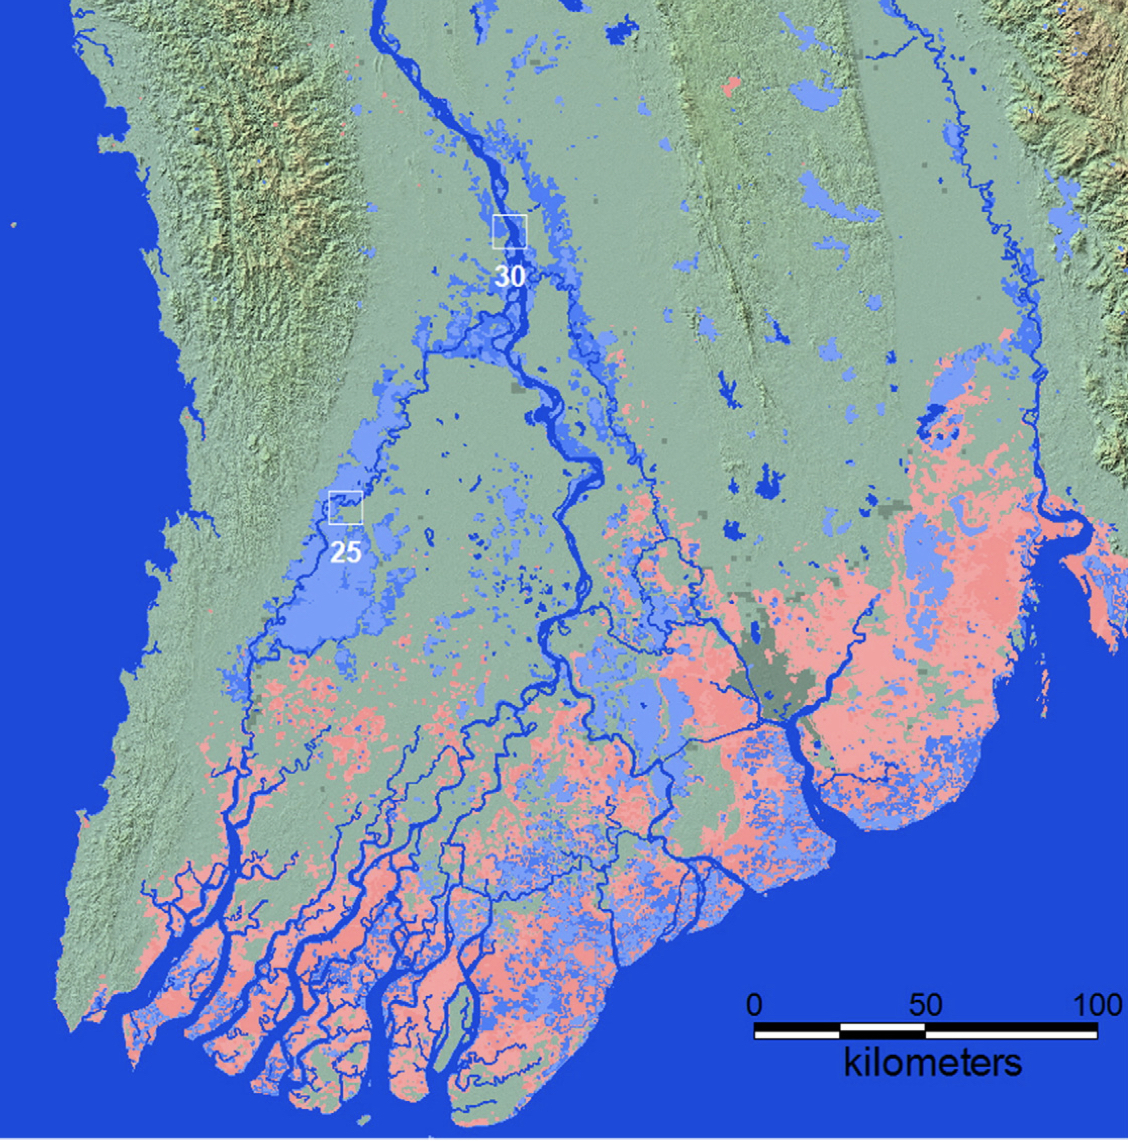
\includegraphics[width=\linewidth]{Graphics/Image8.jpeg}
\caption{Inundation as a result of Nargis (red), compared to typical winter hydrology (dark blue) and average maximum monsoon flood events (medium blue). \red{It would be great if you can move figures to a directory inside images that I had before.}}
\end{figure}

 Nargis is significant to this chapter not only because it had a monumental effect on rice production, but also because it is a prime example of the failures of Myanmar’s military government to protect the lives and economic interests of its residents.
  When Nargis first hit Myanmar, the storm surge flooded approximately 5,200 square km of coastal land and low-lying land, contaminating thousands of rice fields with salt water\red{map?}. An estimated 404, 858 hectares of cropland were inundated by saline water (Seekins, 2009). The storm took over 24 hours to pass through and hit the country on the Western side first, before concentrating over the Southern deltaic region and moving North (Brackenridge et al., 2016). The nature of this storm path was a significant factor in the degree of destructiveness of the storm as the movement triggered a counterclockwise rotation along the shallow southern seabeds of the country, resulting in maximum winds up to 118 km/hour (Brackenridge et al., 2016).

\begin{figure}
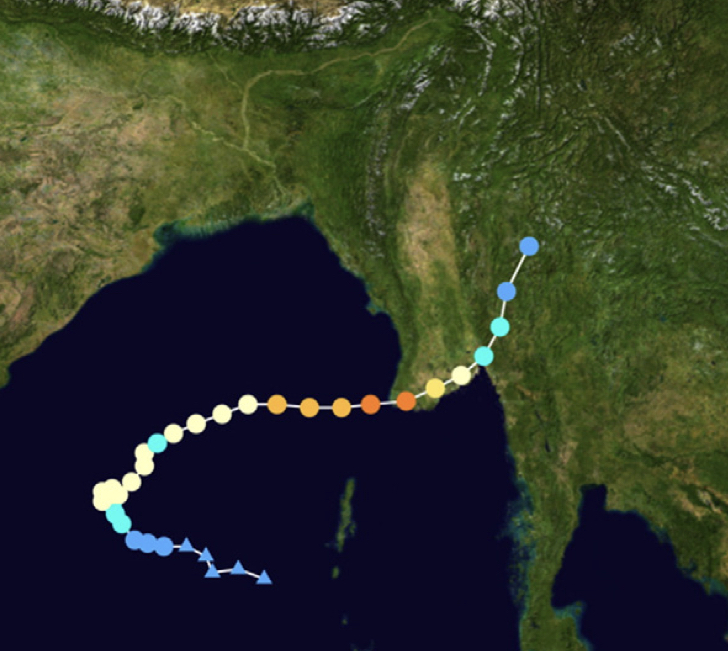
\includegraphics[width=\linewidth]{Graphics/Image9.jpeg}
\caption{Storm path of Cyclone Nargis }
\end{figure}

 Just like any other major flooding event, population growth, deforestation and human construction were identified as long-term causes of the damage inflicted by Cyclone Nargis (Brackenridge et al., 2016). Although these factors are significant, it is important to consider the role of the government of Myanmar in permitting unsustainable dam construction and deforestation to occur, but it is even more important to analyze the country’s disaster response, and to hold the military government accountable for their failures to protect Burmese people.
	In the days following May 3rd, so much chaos and death ensued that the government of Myanmar stopped counting deaths after the toll reached 138,000 (Brackenridge et al., 2016). Although government officials in Myanmar and weather experts worldwide could predict the areas in the projected path of storm, the government failed to communicate the severity of the storm or highlight evacuation routes to the those living in the communities most affected in the coastal south (Brackenridge et al., 2016). Shortly after the cyclone touched down weak infrastructure was quickly overwhelmed. Storm shelters reached capacity and already damaged roads trapped residents in inundated villages (Brackenridge et al., 2016). Many of the deaths tied to Nargis occurred in the weeks following the storm as people in rural areas did not receive proper aid and began combatting disease and starvation (Seekins, 2009).
	Cyclone Nargis did not impact all the residents of Myanmar equally. Poor agricultural workers and other disenfranchised groups throughout the southern parts of the country bore the brunt of the damage. According to the Post-Nargis Assessment, a project conducted by the Special Association of Southeast Asia Nations (ASEAN), 61\% percent of those who died due to Cyclone Nargis and its aftermath were women (Macan-Maker, 2008). Furthermore, thousands of impoverished children were orphaned and had to relocate to cities where they were referred to as “Cyclone Kids.” (Seekins, 2009). Many of these children became subject to exploitation in new metropolitan environments, young girls were frequently forced into prostitution and young boys were often recruited into the Tatmadaw, the Burmese armed forces. 
	In the aftermath of the cyclone foreign aid and global responses to the disaster was met with hostility and ignorance by Myanmar’s military government. When the United Nations called for over 187 million dollars in relief funds the State Peace and Development Council (SPDC) responded that they would accept foreign aid but wanted absolute control over distributions of supplies and made it extremely difficult for relief organizations to get boots on the ground (Seekins, 2009). As time went on Myanmar’s government introduced stricter restrictions on the aid coming into the country. Charity and relief organizations frequently ran into military roadblocks where military forces confiscated food and supplies (Seekins, 2009). The SPDC began facilitating propaganda to discourage organizations from interfering with their response to Nargis. The State-run newspaper “The New Light of Myanmar” declared that the residents of Myanmar no longer needed help obtaining food and supplies because they could get vegetables from the fields and fish and frogs from the creeks (the Irrawaddy, 2008).
	The corruption and overall inefficiencies that were prevalent in the process of delivering aid remained an issue for different relief efforts and government initiatives throughout the country. The SPDC assigned a government organization called the Union Solidarity and Development Association the task of cleaning up the physical damages to infrastructure in the effected regions. The association quickly devolved into a corrupt and harmful presence in many of the communities they were supposed to rebuild (Seekins, 2009). The occupation of removing debris and repairing structures was often left to be organized by community initiatives (Seekins, 2009)\red{when you use the same reference for a whole paragraph, then you might make the subject the "source", so you can highlight the source w/o having to cite very sentance with the same person}. Over the following weeks the international spotlight on the crisis dwindled and food shortages and corruption continued. The Los Angeles Times reported that rice was continuing to be exported out of the country even as thousands of residents of Myanmar were starving domestically (Seekins, 2009)\red{get the original citation from the LATimes!}. The SPDC responded by saying the country was attempting to generate revenue while prices were up globally (Seekins, 2009).
	At first glance the occurrence of Cyclone Nargis may seem like a rarity. Large tropical storms usually do not make landing in the Southern regions of Myanmar, especially compared to regions such as Rakhine, which was hit by severe tropical storms 6 times from 1980 to 2000 (Brackenridge, 2016). This being said, an event as severe as Nargis is projected to reoccur increasingly frequently as the climate crisis\red{I don't know why, but not sure how crisis works in this context -- seems like crisis on top of crisis, is there a better word?} worsens (Brackenridge, 2016). Nargis was extremely damaging to agricultural production in Myanmar, and rice farms in particular were devastated by the event. Much of the agricultural infrastructure that was constructed throughout the 1980s in an effort to improve rice yield was severely damaged or destroyed by the storm. Paddy Land Development Projects 1 and 2, construction projects supported by the World Bank and the Asian Development Bank that implemented drainage systems, polders and sluice gates were made all but irrelevant due to damage. (Omori et al., 2020).\red{begs the question are these projects ever relevant??} Many of the embankments that lined man-made canals or polders were busted as a result of flash floods (Omori et al., 2020). Sluice gates, barriers that are used to control river flow were also overrun in the storm (Omori et al., 2020), The very infrastructure that helps sustain high rates of rice production in Myanmar is clearly extremely susceptible to unpredictable weather in this era of climate crisis.\red{would you say inherantly non-resiliant? be an interesting argument! But perhaps as we discussed today, maybe posing as a question is useful??} Robert Brackenridge, the founder of the Flood Observatory at Dartmouth College, claims that reinforced and sustained flood and sediment management will be necessary to prevent future violent floods in Myanmar(Brackenridge, 2016). Is this sustained management possible considering the political history of Myanmar?


\section{Political History of Rice in Myanmar}
	



\section{Conclusion}





>>>>>>> de527a4eedc4984d93321e9c9721edad286a0ff3



\chapter{Tropical Cyclones in the Philippines}\label{ch:Philippines}

\chapterauthor{Ian Horsburgh}

\red{maybe add to the chapter name: and the Carnot Engine and Climate Change... yes, too long, but you have some cool stuff at the end that needs to be made more visible!}


\section{Tropical Cyclones in the Philippines}

\subsection{A Storm is Coming}
The day is Wednesday, November 6th 2013. In the Visayan Islands, the central islands of the Philippine a\red{A?}rchipelago, the people prepare for a storm. Just days earlier, after a south Asian weather station had begun monitoring a low pressure area east of Micronesia, the storm had been named Haiyan, and been declared a category 5 super typhoon. While Hayian is expected to be the most powerful tropical cyclone ever to hit land, devastating tropical cyclones are not new to the Philippines. One rural Fillipino agricultural worker, Angeles Grefiel, speaks of how past storms have wiped out his crops, leaving him with no money to provide his children with a healthy diet. ``We have generations of children that have grown up without having proper access to the right types of food,'' says Grefiel, a sentiment echoed by Evangeline Aloha, a resident of Leyte Province in the central Philippines, who worries she will have no income if the harvest is wiped out by the storm. As certain cash crops are easily wiped out by heavy rain, many farmworkers like Evangeline and Angeles are ``so vulnerable to disasters that when one strikes, it takes them further and further into that cycle of poverty,'' says a local social worker, also in Leyte Province. To see why certain crops are planted and how they make the country so much more vulnerable to tropical cyclones, we must take a look back on the history of agriculture in the Philippines. \red{great intro!}
  
\subsection{Agriculture and Cyclone Vulnerability?}
Rural Filipino farmers are vulnerable to tropical storms in part due to their integration into worldwide markets. In particular, famine is often a product of the conditions surrounding access to food. ``Famine must be seen not as an absolute scarcity of food in particular regions, but rather as a loss of one’s\red{fix apostrophe} entitlements\red{does the word have a different meaning than to US uses?} to food and/or the means of subsistence,'' writes \citet{warren2018typhoons}. As for Fillipino farmers, this loss of entitlement goes back to the colonial era. Throughout history, rice has been a staple crop in the Philippines. Due to the favorable and temperate climate, Fillipino farmers were able to harvest rice twice a year, while simultaneously planting root crops such as sweet potato. When typhoons ``created severe food shortages for those who grew rice, these root crops became...the ‘\red{look up how to do quotes and apostroshe's in \LaTeX, you have it right in some sections\ldots, the problem for me when I cut and paste in to Rstudio}refuge of the poor’''\citep{warren2018typhoons}. However, in the nineteenth century, this dynamic began to change. 
	Spanish colonization of the Philippines began in the 1500\red{’}s, although major agricultural change, especially as it relates to globalization and integration into market economies started in the early 19th century. This began with ``the Spanish practice of rewarding the Catholic orders for their conversion efforts with land,'' which ``turned the church into the largest landlord in the islands''\citep{ventura2016small}. Spanish catholic landlords then divided up their land, and under this system, ``Inquilinos (tenant landlords) paid annual rents for lands they then subdivided among sharecroppers, who often further subdivided their portions, which would be worked by families living in a central town near the fields''\citep{ventura2016small}.\red{any figure could break up the text here} This system was a major step towards the integration of Filippino farming into the global economy, due to the fact that ''as estates commercialized, they increasingly shared management with Chinese-Philippine mestizo businessmen,'' who had access to British capital \citep{ventura2016small}. When America resumed colonial control following their defeat of Spain in the Spanish-American war in 1898, there were a number of changes to this system, but integration into global markets continued. At the  beginning of the United States’ rule,\red{super interesting!} the new leadership feigned effort to give farmers independent ownership over their land, but just two years later abandoned this effort, apocryphally citing lack of interest in this initiative by the peasants \citep{ventura2016small}. Former president William Howard t\red{T}aft, the civilian governor of the Philippines from 1901 to 1904, then changed direction entirely, saying that ``easing the homestead law’s limitations on corporate ownership to 2,500 acres\red{\ldots is better spacing}...was a much better path to development.'' Following this reversion to a similar corporate control as implemented by Spain, ``prevailing inequalities of landholding and rural wealth during the Spanish period multiplied under US rule.'' \citet{ventura2016small} summarizes the issue, saying that the United States’ ``failure to establish independent homesteads was akin to other alleged shortcomings in hygiene and sanitation, education, and banking, thus justifying the US presence in the islands,'' and consequently ``ownership for large scale plantation agriculture.'' US Civil Service Advisor Roy Franklin Barton talks of the American reforms in the agricultural region of Ifugao, describing how the new ``availability of wage labor jobs'' makes way for ``the introduction of money into the province replacing the old rice currency,'' and thus ``the integration of a market economy'' \citep{klock1995agricultural}. Thus, Spanish and American policies in the Philippines transitioned the country from local to large scale plantation agriculture.\red{add a line if you want a new paragraph}
  This incorporation into large scale plantation agriculture and world trade had large impacts on the vulnerability of the area to natural disasters, such as typhoons ``There is persuasive evidence that peasants and farm laborers became dramatically more pregnable to natural disasters after 1850 as their local economies were violently incorporated into the world market,'' writes \citet{davis2002late}. ``The vulnerability of tropical agriculturalists to extreme climate events after 1870 was magnified by simultaneous restructurings of household and village linkages to regional production systems.'' In refuting claims that farmers chose to adopt to this new age agriculture because it provided a better life, Davis argues that “Recent scholarship confirms that it was subsistence adversity (high taxes, chronic indebtedness, inadequate acreage, loss of subsidiary employment opportunities, enclosure of common resources, dissolution of patrimonial obligations, and so on), not entrepreneurial opportunity, that typically promoted the turn to cash-crop cultivation.”\red{great quote, need page number}
This cash crop cultivation became the primary type of farming in the Philippines by the mid 19th century, and even farmers who still owned land were increasingly ``encouraged to plant cash crops of abaca, copra, tobacco and sugar, and were often forced to sell rice below market prices''\citep{warren2018typhoons}. 
By the 20th century,much of the rice still produced by the Philippines was exported to China, while poor Filipinos lived ``almost exclusively on imported rice, tubers and corn'' \citep{warren2018typhoons}. Thus, rather than the pre-colonial model of growing rice and root crops, a model that was fairly robust in the face of typhoons, farmers in the colonial Philippines who were encouraged to grow cash crops and buy imported rice, as well as those who now worked plantations for a wage, were left with no money and thus no food when cash crops were wiped out by typhoons. As many cash crops rely on long fertile growing seasons for harvest, and thus were much more easily disrupted by storms, ``subsistence farmers, who increasingly chose to cultivate cash crops, counting on a better standard of living,\red{can you make a diagram of this? maybe not, just think about it} often found they had no visible means of sustaining themselves, because of the ‘economic predicament’ triggered by typhoons,'' writes \citet{warren2018typhoons}, again. Thus, in the shift from a diversified to monocrop economy, agricultural, and thus economic disaster became ``a fact of life'' In sum, as colonial powers such as the United States and Spain implemented policy that shifted Filippino agriculture toward cash crop cultivation within worldwide markets, and away from a local multicrop system, the country became more vulnerable to typhoons.\red{really interesting history!}


\red{I think this might be a good place to talk about how cyclone work...}

\subsection{Ready or Not}\red{not very descriptive as a subsection name\ldots}
  As the supertyphoon Hayian approached the Philippine islands, the government scrambled to alert those in danger, but to various degrees of success. While some in danger, like Retche Ycoy, did not receive any warning--``We didn’t expect this was going to happen. We were just sitting around in our house and the wind suddenly started''--others, like 62 year old taxi cab driver Eduardo did not realize what the warnings meant. Recalling the situation, he said, ``What I understood was that there would be a strong wind. We never understood what a storm surge meant.''\red{what's the source of these quotes?}  Others still, like Celina Camposano of Leyte were told to evacuate. While these responses vary from having heard no warning whatsoever to being evacuated and sent to higher ground, they all share one sentiment: their past experiences with tropical storms did not prepare them for what was about to come. \red{paragraph}
  From educating and warning those in danger to helping those affected find food and shelter, the federal Philippine response to tropical cyclones like Haiyan has many obligations. In this section, we will investigate what this response entails, what areas it is successful in, and how it can improve.\red{seems odd that this is present tense, but I can think of ways that this work in the intro, but not sure about now\ldots} While ‘disaster mitigation’ can mean many things, we \red{\st{will}} separate it into post disaster recovery, and pre-disaster preparation. 

\begin{figure}
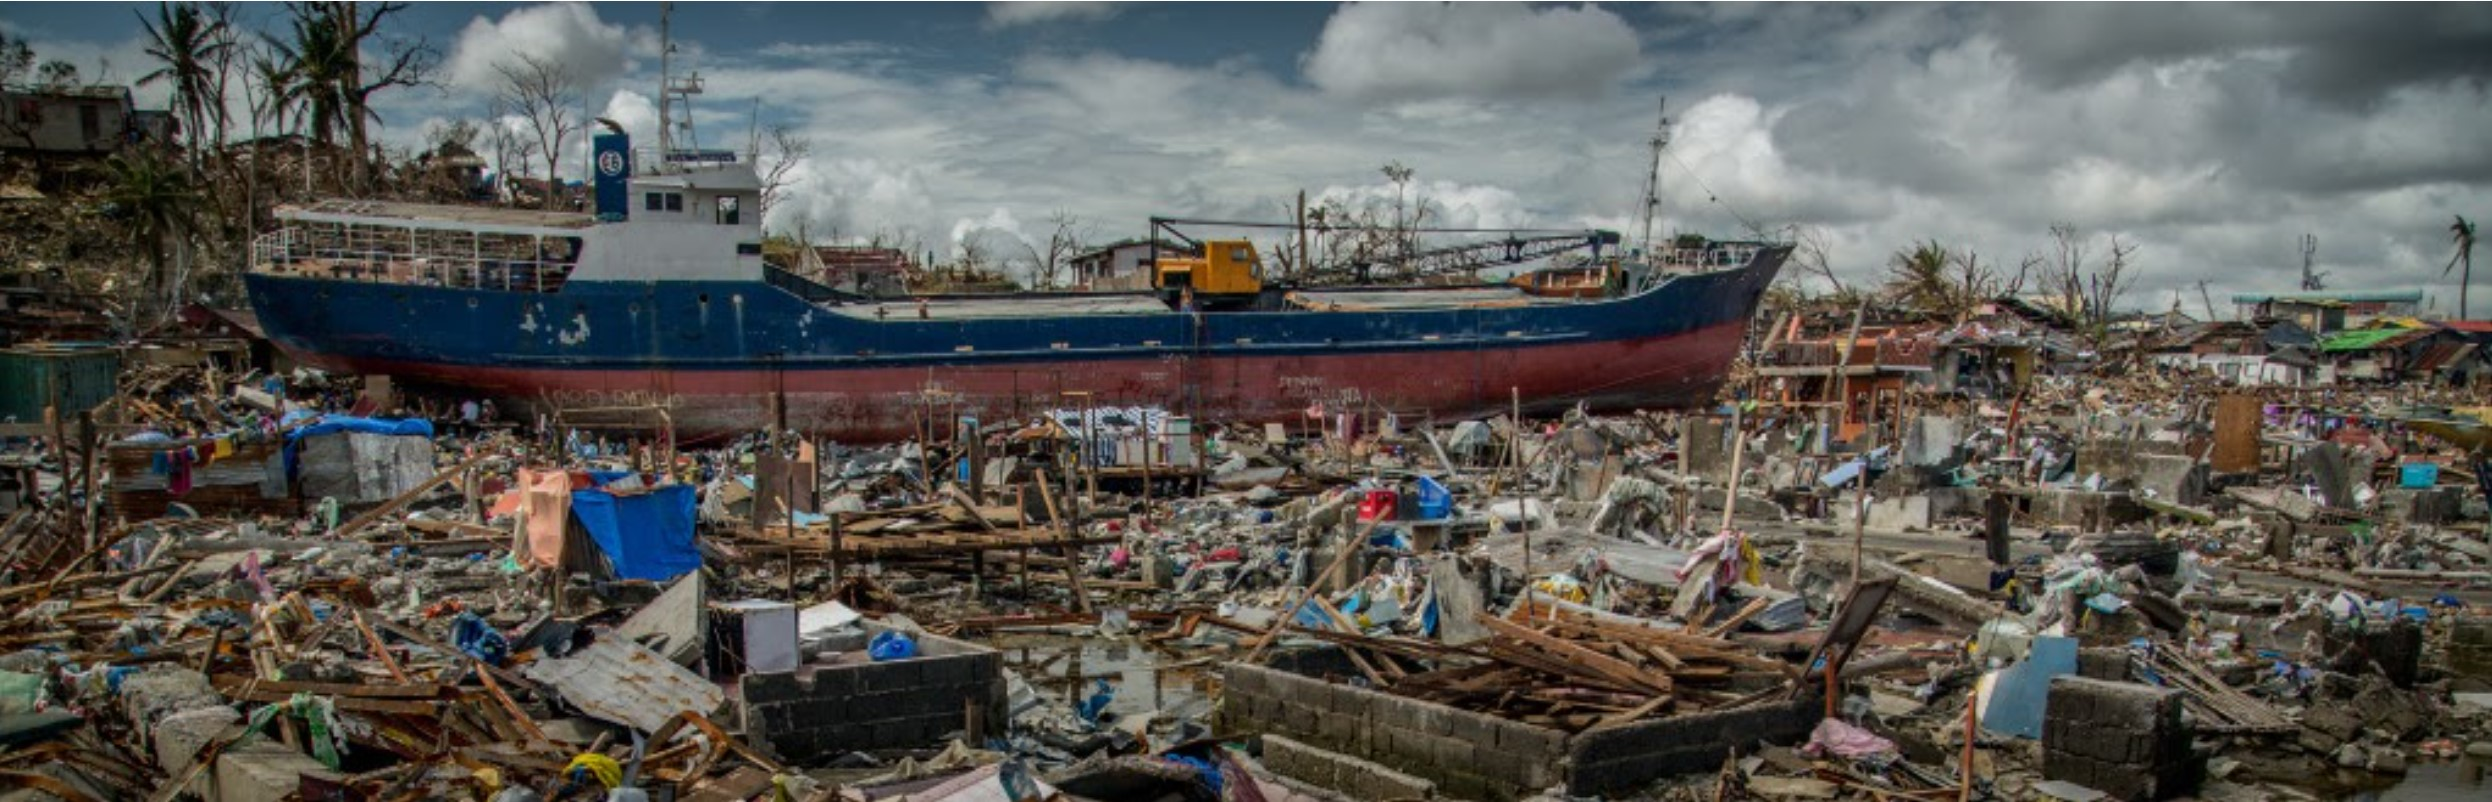
\includegraphics[width=\textwidth]{images/tropical-cyclones/boat.jpg}
\caption{A Ship is washed ashore in Tacloban City
\red{let use a more descriptive label remember there are 16 chapters! also need to be one word or hyponated word.}} 
\label{fig:figure-1}
\end{figure}

\red{to reference figure\ldots Figure~\ref{fig:figure-1}, bute needs a better reference name!}

\subsection{Philippine Disaster Mitigation}
  The Philippines has a number of programs aimed at disaster relief, as seen in figure 10.2.\red{add reference to auto number}Typhoon Haiyan, locally know as Typhoon Yolanda, was disasterous. With 195 mph 1-minute sustained wind speeds, Yolanda\red{confusing to have two names} was the most powerful storm ever to make landfall at the time. With 6300 people dead, and a million houses destroyed or damaged, the Philippine government had much work to do to provide relief for those that survived the devastating storm.
  Immediately after the storm, the Department of Social Welfare and Development (DSWD) provided shelter assistance to many displaced households. For nearly 60,000 household, this came in the form of emergency shelter kits. Although the kits were helpful in providing emergency shelter, the number of families that received the emergency shelter assistance was limited due to an insufficient supply of kits delivered. \citep{bowen2015social}. In addition to these kits, DSWD helped to coordinate the delivery of 136,267 roofing solutions to help with roofs that had been blown off, like Papoose’s. Concurrently, other families were sent to shelters or bunkhouses, and by the 5th month of the response, many of the families who were originally living in emergency shelter kit housing were transferred to more substantial bunkhouses as well. However, this relief housing was not sufficient for all. Another program implemented by DSWD was Food for Work.

\begin{figure}
\centering
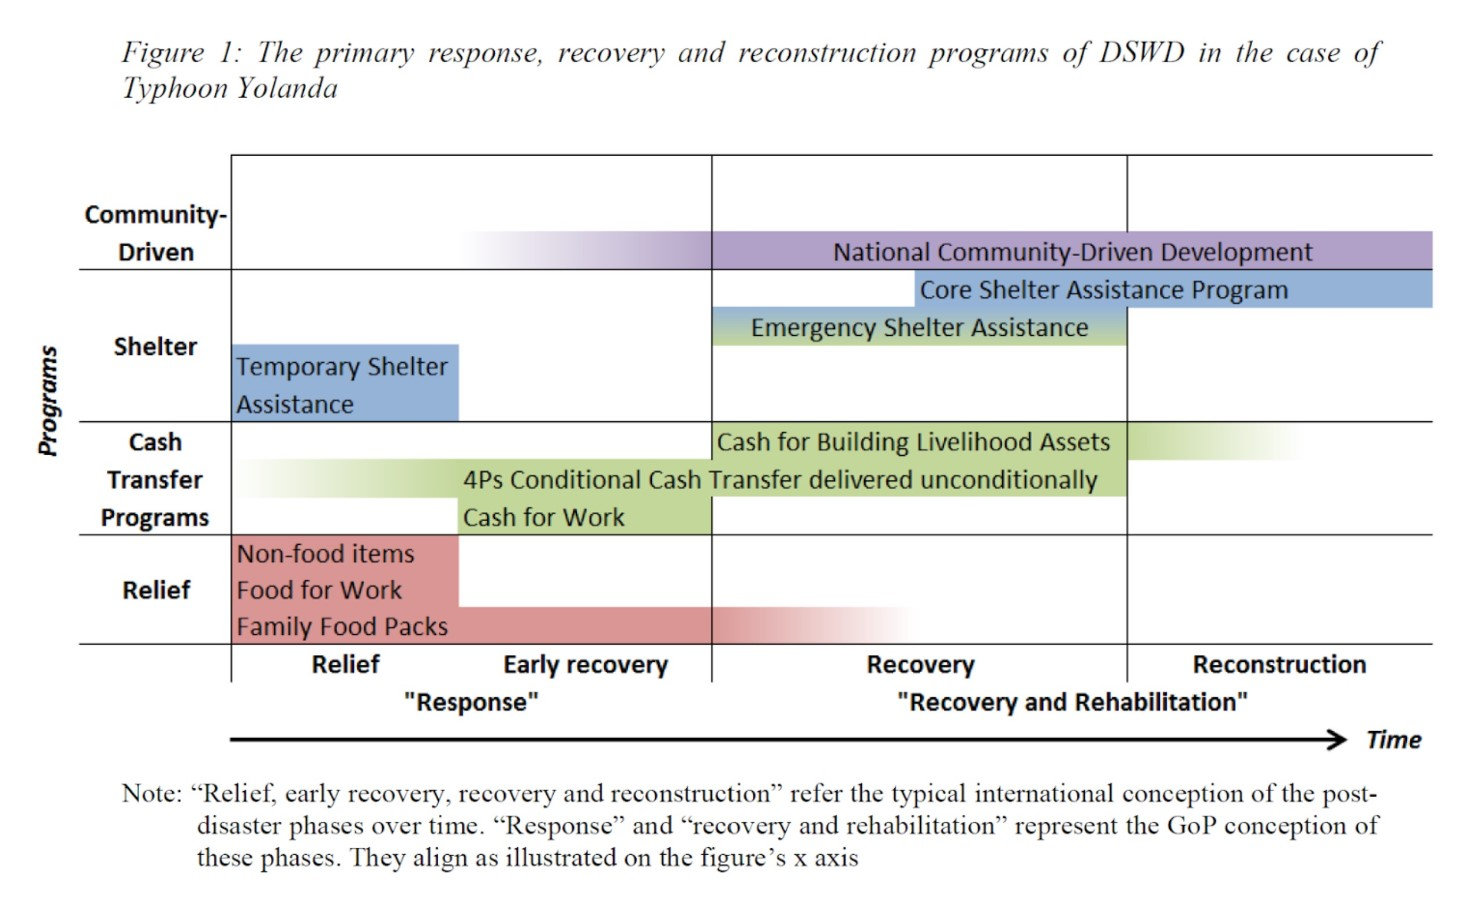
\includegraphics[width=\textwidth]{images/tropical-cyclones/reliefchart.jpg}
\caption{DSWD Relief Programs}
\label{fig:figure 2}
\end{figure}


  In the DSWD’s food for work program, ``Beneficiaries were given food packs in exchange for the provision of their labor to assist in the repacking and distribution of relief goods'' \citep{bowen2015social}. This both helped to expedite the processing and distribution of food packs, and employ/guarantee food for those who lost their job as a result of the tropical cyclone. As the needs of the workers moved beyond immediate shelter and survival, this Food for Work program was replaced with Cash for Work. In the Cash for Work (CFW) program, which continued long into the relief effort, jobs included ``loading/unloading of goods, repacking of relief goods, food preparation, sorting and inventory of damaged property, clearing of debris, coastal clean-up, and canal dredging, among other things'' \citep{bowen2015social}. By 2014, 15,188 people were participating in CFW, which ``helped to provide much needed additional assistance to DSWD relief programs on the ground, while providing beneficiaries with cash based assistance''\citep{bowen2015social}. Programs like Cash for Work, however, would not have been possible without existing cash transfer infrastructure.
  The DWWD, with the help of humanitarian organizations, capitalized on strong pre-existing social welfare programs, especially cash transfer infrastructure, to provide monetary relief in the wake of Hayian. In total, ``Four agencies alone in the inter-agency response distributed around US\$34 million, benefitting 1.4 million disaster-affected people''\citep{bowen2015social}. This money was distributed in various ways, with around 70\red{\%} percent of cash transfers being conditional (Cash for work, etc), and 23 percent being unconditional. Although this system works well, the Phillippine government should learn from and refine this cash distribution process for future disasters, as a number of issues in ``coordination leading to coverage gaps and duplication'' of funds were reported during the Hayian relief period\citep{bowen2015social}.\red{maybe define the problem then tell how to solve?} In addition to government aid, local relief and community driven development  was key to post-Haiyan recovery.\red{we could create a table of activities and their evaluation and recommended changes, make be better than to have all in text?}
  Community driven development refers primarily to the subsection of the DSWD called the National Community Driven Development (NCDD) program that operates primarily on local levels and was established in 2002 to help alleviate rural poverty, especially surrounding disasters. In addition to implementing general infrastructure, the NCDD is well poised for disaster relief due to its geographical breadth and ``has a well established network of community facilitators and community volunteers on the ground''\citep{bowen2015social}. Following Yolanda, the NCDD played a large part ``in the rebuilding/rehabilitation process'' of affected communities by taking on projects such as rebuilding roads, paths/trails, schools, flood/drainage control structures, water systems, and health stations. Thus, ``The Yolanda experience has also demonstrated the important role that community driven development programs can play in the recovery of poor and vulnerable people from disasters''\citep{bowen2015social}. Finally, the Core Shelter Assistance Program helped those affected by the storm find housing. 
  In an effort to build more secure and resilient housing, the DSWD implemented the Core Shelter Assistance Program (CSAP), which aims to establish permanent safe housing for the rural poor. Following emergency housing after a storm, the CSAP builds ``a standardized two-room structure that is built to withstand 220 kmph wind-speeds''\citep{bowen2015social}. As a testament to the durability of these shelters, a local Social Welfare and Development officer stated that ``The core shelter units built through the CSAP of DSWD are still standing even after the mighty force of Typhoon Yolanda...all 80 units built in 1991, 2000 and 2010 in Barangays Cansuso, San Marcelino, San Sebastian, and San Guillermo remain standing''\citep{bowen2015social}.\red{I don't know anything about construction, but that seems impressive! Is it?} Thus, this program provides robust housing that not only serves as relief for typhoon victims, but actually serves to mitigate future damage caused by natural disasters. 
  Overall, the Philippine government has established a fairly robust system for addressing typhoon relief, combining immediate food and shelter relief with one of the best social protection programs in the region, which helps many residents with both immediate survival and monetary subsistence. However, despite these systems to address relief, many residents still live close to the poverty line. As seen in the figure 10.3\red{autoref using a refernce to a label}, 44\% of Philippine residents experience poverty at least once, and of those that do, 2 out of 3 are in and out of poverty, often triggered by typhoons like Yolanda. While the systems described above do well to provide relief following a tropical storm, thus making the poverty triggered by the storm only transitory, other adaptation and mitigation measures could help reduce the need for such extensive post disaster support as well as decrease the number of deaths immediately caused by typhoons. While some measures described above, such as robust housing, function in this way, there are a number of other measures that can be taken to reduce the effects of tropical cyclones.
  
\red{check this out\ldots, is there something like this for the philippines? \url{https://cran.r-project.org/web/packages/hurricaneexposure/vignettes/hurricaneexposure.html}, if not it begs the question, great educational tool, perhaps}

\begin{figure}
\centering
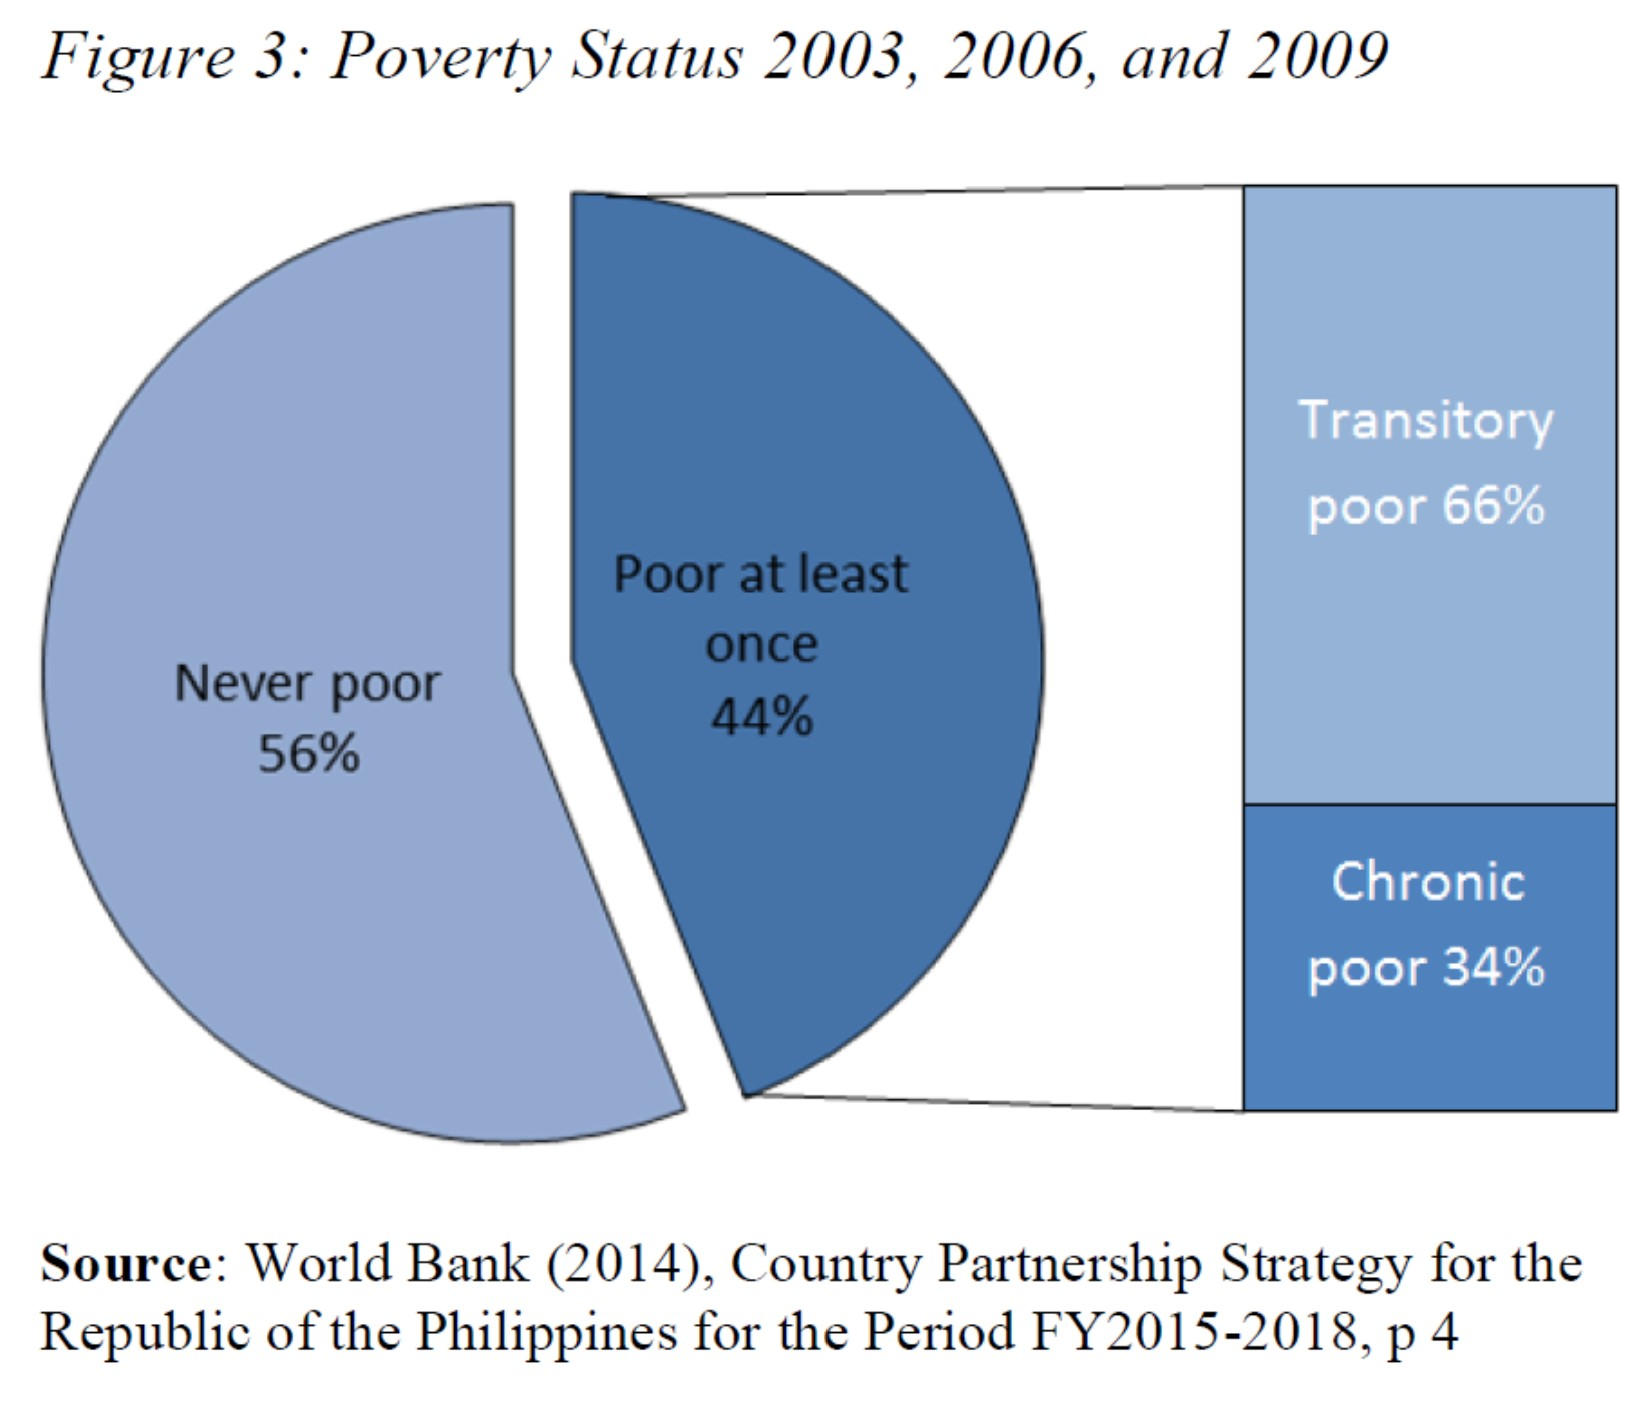
\includegraphics[width=8cm,height=24cm,keepaspectratio]{images/tropical-cyclones/povertystatus.jpg}
\caption{\red{change the reference label to something more descriptive and then we can use a reference in the text.}}
\label{fig:figure 3}
\end{figure}

\red{new section/subsection?}
  Disaster mitigation takes many forms, from long term prevention to recovery. As we have previously discussed recovery and post-disaster mitigation, which the Philippines has demonstrated great competency in, we will now talk about prevention, a sector which the south asian archipelago will need to invest in to mitigate damage caused by future storms. The first form this investment could take is protecting natural land features.\red{is there a science to disaster relief that we could add?}
	While man made structures such as walls and barriers offer some protection and psychological reassurance, they are not an ideal long term solution to cyclone mitigation \citep{king2010disaster}. This stems from a few factors, the first of which being their high maintenance costs, which leads to neglect, and thus causes a dangerous scenario of false security, as was observed in hurricane Katrina in New Orleans in 2005. Another downside of man made structures is that if they are breached, they often keep water in, creating a ponding effect that ``severely constrains response and recovery''\citep{king2010disaster}. Instead of man made infrastructure, many researchers emphasize the importance of retaining natural land features.
	Natural features such as coral reefs, mangroves, and dune ridges ``are extremely effective in controlling storm surge flooding,'' writes \citet{king2010disaster}.\red{seems like this could / should be a new section to focus on `best practices'} While coral reels are able to absorb ``some of the power of tropical cyclone wind-generated waves and surges'' before they hit land, mangroves are crucial to providing relief as they are extremely resilient to tropical storms, and often provide shelter and safety to people and boats around them \citep{williams2007lesson}. While only 20\% of the once 500,000 mangroves in the Philippines remained by the early 1990’s, local and national authorities observed this effect of mangrove protection from tropical storms, and have planted 600,000 mangroves since 1996. In addition to typhoon protection, this has had other benefits such as improved fishing and ecotourism \citep{williams2007lesson}. \citet{williams2007lesson} notes, however, that although Philippine legislature in planting mangroves for cyclone protection could be considered a success story, enforcement is ``often wanting,'' and continuous efforts must be made to maintain the progress the country has made in this respect. The final natural feature that has been observed to help prevent typhoon damage is coastal dunes, behind which ``lagoonal wetlands absorb immundation''\citep{king2010disaster}. Unfortunately, these are in great danger, as ``coastal zones have been cleared, settled, and built over''\citep{king2010disaster}. Thus land use planning and legislature are crucial to maintaining, or many cases such as that of mangroves, rebuilding natural infrastructure to mitigate typhoon damage. In addition to infrastructure, education is imperative to disaster mitigation. 
	Mitigation measures have little to no impact ``if the people do not know the hazard risk'' or ``are unaware of evacuation routes, sheltering strategies, and appropriate response to warnings,'' as demonstrated by Eduardo and Maria \citep{king2010disaster}. ``Many people who may have been through a Category 1 or 2 cyclone have no awareness from that experience of what a Category 3 or 4 will do,''  writes \citet{king2010disaster}, again. As the pre-existing idea of what the storm will look like may contradict official reports, vulnerable populations must be educated on what different categories of storms mean, and what responses are appropriate for the divergent levels. Once these warnings are understood, a robust warning system is extremely helpful in preventing injuries and casualties due to storms. In sum, the Philippine government has created a robust post-disaster relief system that encompasses housing, food, and work. However, to mitigate the damage caused by future storms, the country must invest in protecting natural features such as mangroves, coral reefs, and coastal dunes, as well as strengthen education programs on tropical cyclones.
	
	\red{Okay, I like this, but let's integrate into the text\ldots, perhaps this could be inerted into the areas where you talk about colonilizatoin and talk about long term land use affecting resilience of mangroves?? Maybe too much to force, but it might break up with history with some ecology in a nice way and demonstrate some vulneratility linked to colonial land use changes -- if that actually happened???}
		
\subsection{A Changing Game}\red{perhaps a better heading to be more transparent}
  Compounding issues of lack of education\red{lack of education is a strnge beast, some can 'see' this as a lack of interest by residents, lack of motivation, others will blame gov't. I wonder if we can make sure the reader gets your intention here} on tropical storms is the fact that the nature of these storms is changing. Some residents, such as Maria Flora Orbong of Tacloban City understood what the storm surge meant, yet was still underprepared for storms of Haiyan’s magnitude, remarking that ``We knew that a strong typhoon was coming but we didn’t really expect the water [levels] to rise that high …\red{\ldots} our neighbors evacuated but we thought we were safe. We were in the middle, surrounded [by cement houses].'' Less than an hour after the storm hit the Island, however, things were far from expected. ``The waves rose to six or eight metres (20 to 26 feet)...many people started to escape but the ships washed up and many people died,'' recalls Orbong. Celina Camposano of Leyte echoes the novelty of this storm, saying ``We’ve never experienced something like this before … \red{\ldots}we’ve never had to evacuate before.'' While some of this gap between expectations and reality is due to lack of education on cyclone threat, another reason locals were unprepared for what typhoon brought was that the nature of these types of storms are changing. To understand this change, we must look at how tropical cyclones work and how they are affected by climate change.
  
\subsection{Tropical Cyclones and Climate Change}
Tropical cyclones, referred to as typhoons when taking place over the Pacific Ocean, occur in southeast Asia primarily in the late summer and fall. Distinct from the monsoon season, which describes the prevailing wind that causes a predictable rainy season in the summer months, typhoons are isolated and severe events, sometimes accounting for more precipitation than the entire monsoon season brings\red{interesting!}. Typhoons typically form in warm equatorial ocean waters, as the warm air near the surface rises, leaving an area of lower pressure below. 
Soon, a cycle forms, with surrounding air moving into the lower pressure region before heating up and rising itself. Once the risen air cools off, it forms clouds, which are then fed into the cycle, as seen in figure \red{10.4} Other characteristics often accompany this air and cloud flow, such as torrential rains and a storm surge which can elevate the sea surface 20 feet and cause widespread flooding. 

\begin{figure}
\centering
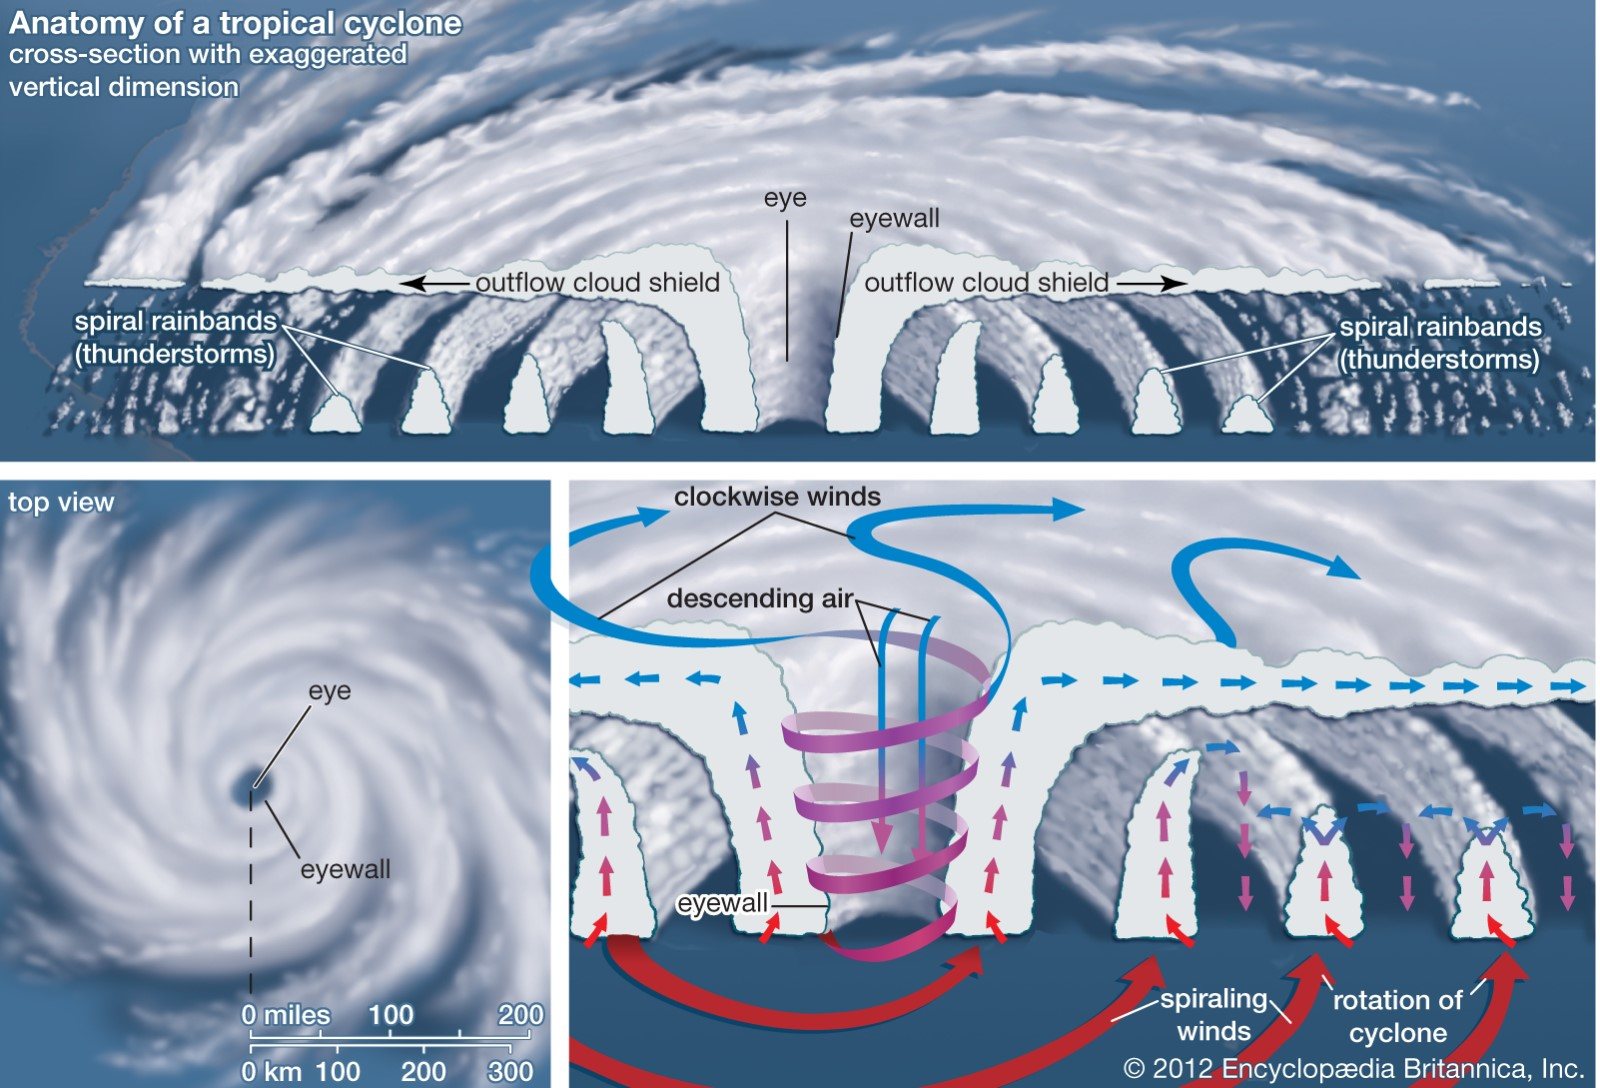
\includegraphics[width=8cm,height=24cm,keepaspectratio]{images/tropical-cyclones/cycloneanatomy.jpg}
\caption{}
\label{fig:figure 4}
\end{figure}

  To represent how these tropical cyclones operate, climate scientists often employ the Carnot Engine model, a theoretical thermodynamic cycle that provides an upper limit on how powerful a storm can be \citep{emanuel1987dependence}. The model depicts fluid\red{air is modelled as a fluid, but I wonder if readers will get that? and why?} that performs work (a measure of energy transfer that occurs when an object is moved) on its surroundings while undergoing four stages, the fourth of which returns to the first, making it cyclic.\red{is there a figure that shows this? Are there some equations that might demonstrate how the model works?  I wonder if we can create a little simulation? \url{https://www.researchgate.net/figure/Carnot-cycle-Figure-5-Structure-of-a-hurricane-Air-is-cooled-through-convection-by_fig1_323693275}} In the case of a cyclone, this fluid takes the form of a mixture of dry air, water vapor, and suspended condensed water, all of which are in thermal equilibrium (the same temperature). However, as the ocean and the atmosphere are in thermal disequilibrium (not the same temperature), the ocean loses heat to the atmosphere by evaporation of water, which has a large heat of vaporization \citep{emanuel2006hurricanes}.\red{this is super interesting and deserves more space if you can figure it out!}
  The carnot cycle uses this heat flow as an input to estimate the maximum power output that could be produced if the storm was perfectly efficient. Although this perfect efficiency is impossible, the carnot cycle is useful to give an upper bound on storm power, operating as described in figure $10.5$.

\red{you should cite earlier chapters...}
  A quick aside on the greenhouse effect: You’ve probably heard the term ``the greenhouse effect'' thrown around, but if you forgot what it is or never learned, here’s a brief summary. Of the light radiated by the sun, 30\% is reflected by the clouds or surface and the rest is (mostly) absorbed by the earth. The earth then transmits energy up by radiation and convection currents, some of which are absorbed by certain elements in the atmosphere such as water vapor, methane, and carbon dioxide. These molecules are known as greenhouse gasses because they act on the climate as a greenhouse does on a garden, trapping heat in the atmosphere.
As a higher concentration of greenhouse gases in the atmosphere leads to a higher temperature, the disequilibrium between the atmospheric temperature and the water increases, thus amplifying the heat flow powering the carnot cycle, which results in a higher upper bound for the intensity of the cyclone\citep{emanuel2006hurricanes}.

\begin{figure}
\centering
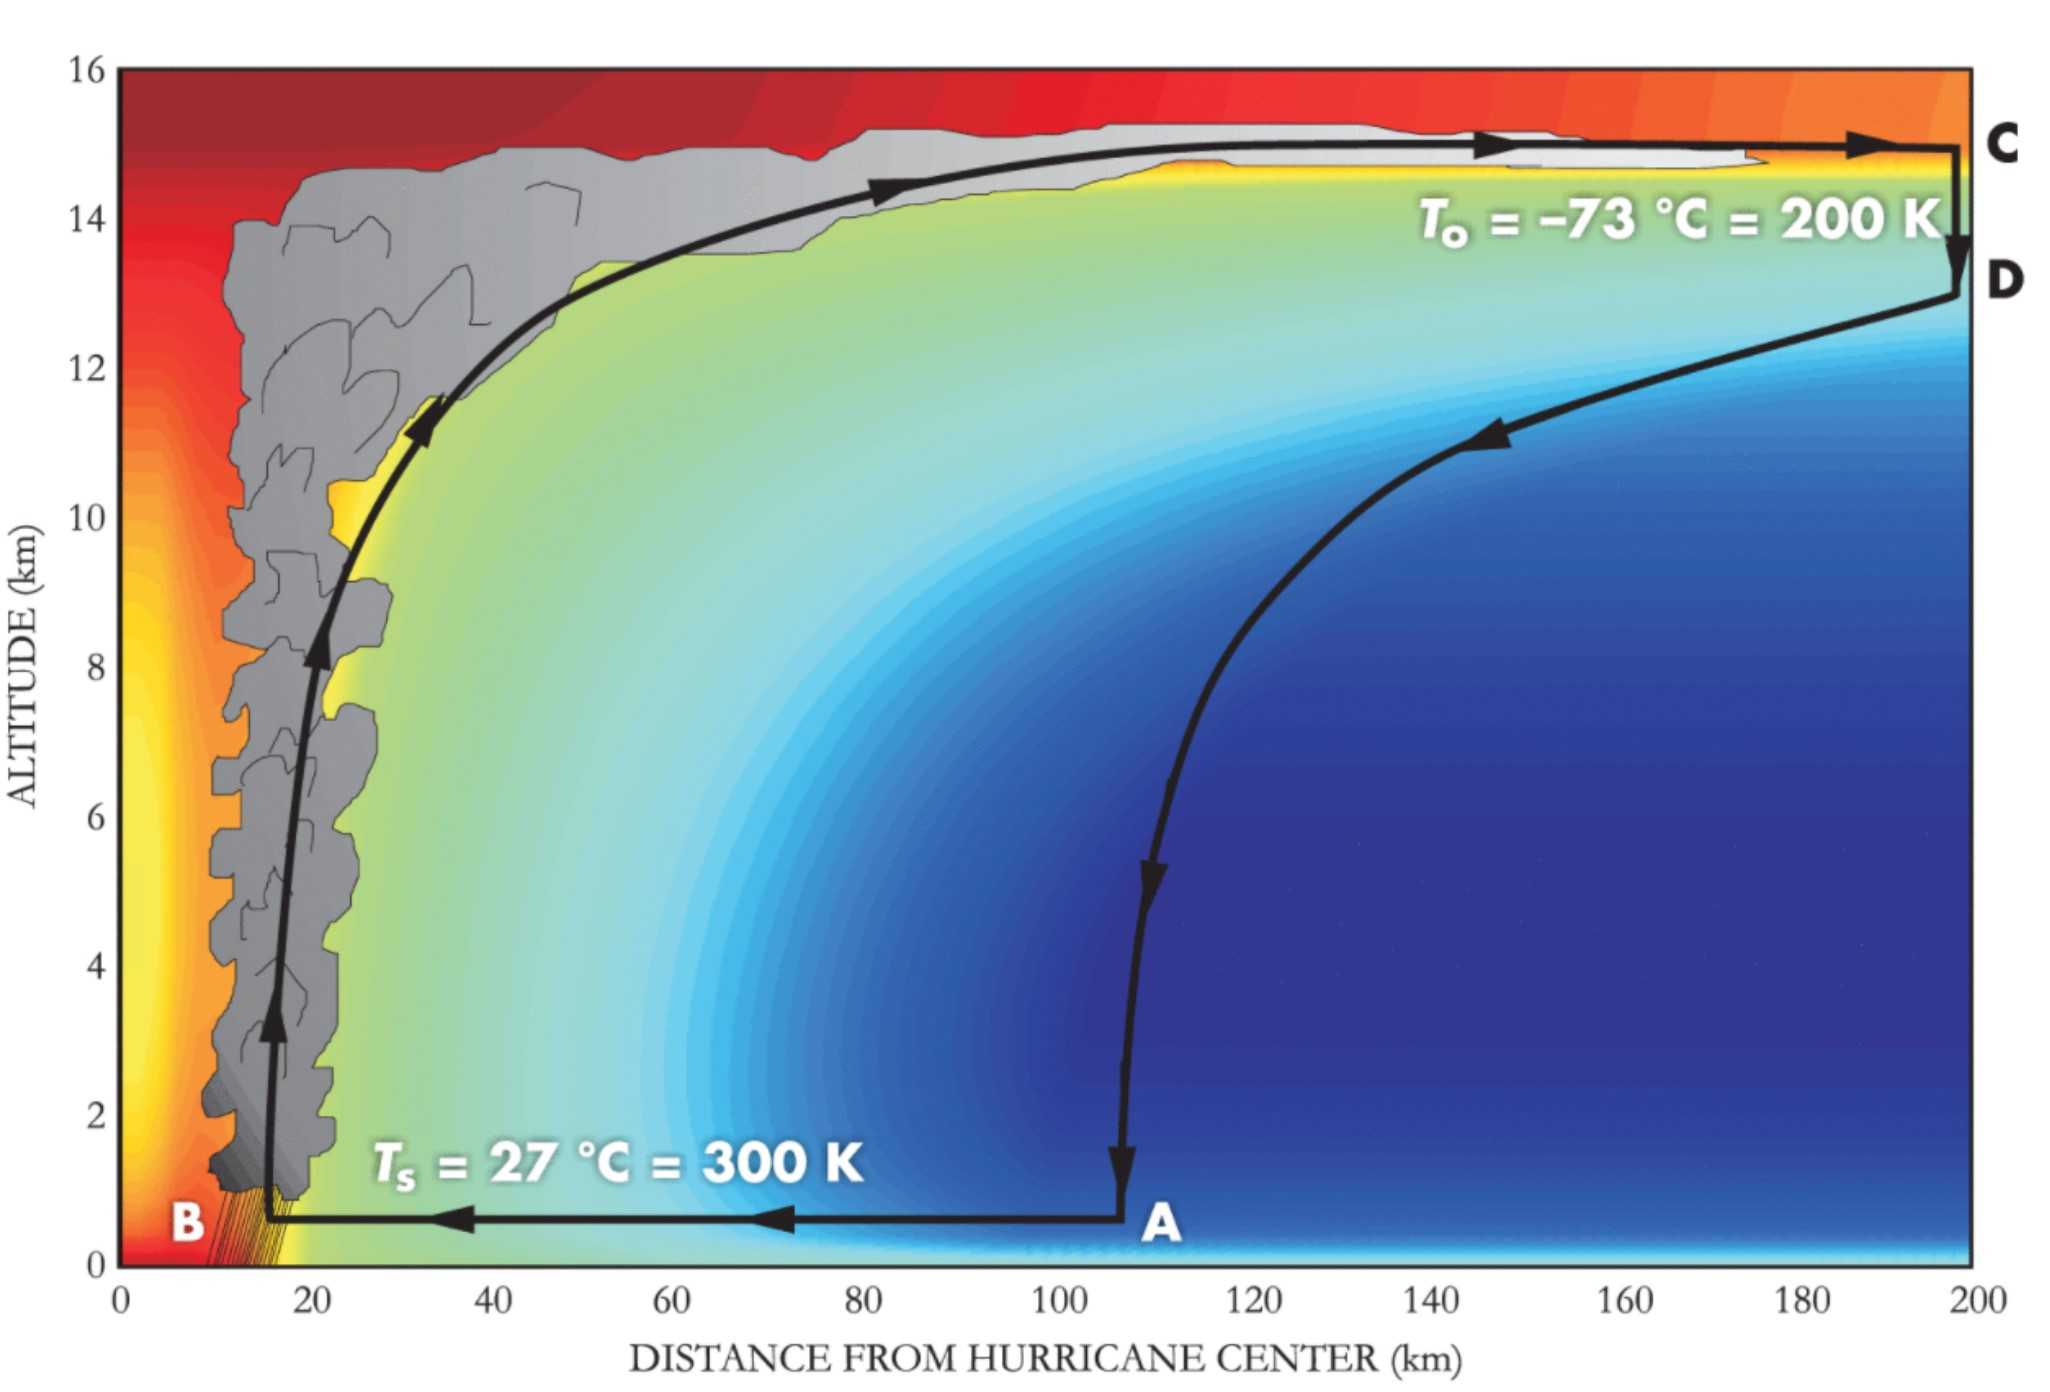
\includegraphics[width=12cm,height=36cm,keepaspectratio]{images/tropical-cyclones/carnotcycle.jpg}
\caption{}
\label{fig:figure 5}
\end{figure}

All this physics on tropical cyclone modeling provides good intuition for why an increase in greenhouse gas concentration in the atmosphere could lead to more powerful storms, but to really quantify this change, we must look to climate simulations and statistics. To investigate one statistic that is particularly pertinent to quantifying cyclone power and potential destructiveness, we look to meteorologist Kerry Emmaneul’s work. In his 2005 article Increasing Destructiveness of Tropical Cyclones, \citet{emanuel2005increasing} noted that ``Basic theory,'' such as what we have looked at with the carnot cycle, ``establishes a quantitative upper bound on hurricane intensity, as measured by maximum surface wind speed.'' Observing that ``the actual monetary loss in wind storms rises roughly as the cube of the wind speed,'' Emmanuel \red{would giving a short biography of this person, create more interest in his/her work?}created the Power Dissipation Index, which he defines as:
$$PDI \equiv \int_0^t \sf{V_{max}}^3 \, dt$$
A quick refresher in calculus: the integral represents the area under a curve, so in this case the curve would be a graph of the maximum sustained wind speed of a storm over time (Velocity cubed), and the integral of V3 would be the area under this curve starting at the beginning of the storm $\sf{t{0}}$ = 0, and ending at time t. This is shown by the 0 and t at the bottom and top, respectively, of the integral symbol. \red{great!, can we create a simulation and show PDI as it relates to t or v?} A simplification of a previous statistic that was problematic as it input data\red{what is the input data needed?  I assume that t and V are not enough?} that was seldom recorded, \citet{emanuel2005increasing} notes that ``this [new] index is a better indicator of tropical cyclone threat than storm frequency or intensity alone.'' Because it does well to estimate the damage of tropical cyclones, only requires one input\red{but not measured?}, and is easy to evaluate, it is often used to represent tropical storm damage.
	Using PDI to gauge storm intensity, numerous studies conclude that tropical cyclone intensity will increase under climate change \citep{zhang2017response}, \citep{emanuel2013downscaling}, \citep{chen2021typhoons}. To apply physics to large scale climatological events, scientists use climate models, which divide up the earth's surface into grid cells, and use complex equations based on fundamental laws of physics, fluid motion, and chemistry to describe how energy and the materials within the grid move through it \citep{noaaclimate.gov}. A visual of this type of model is given in the figure below.

\begin{figure}
\centering
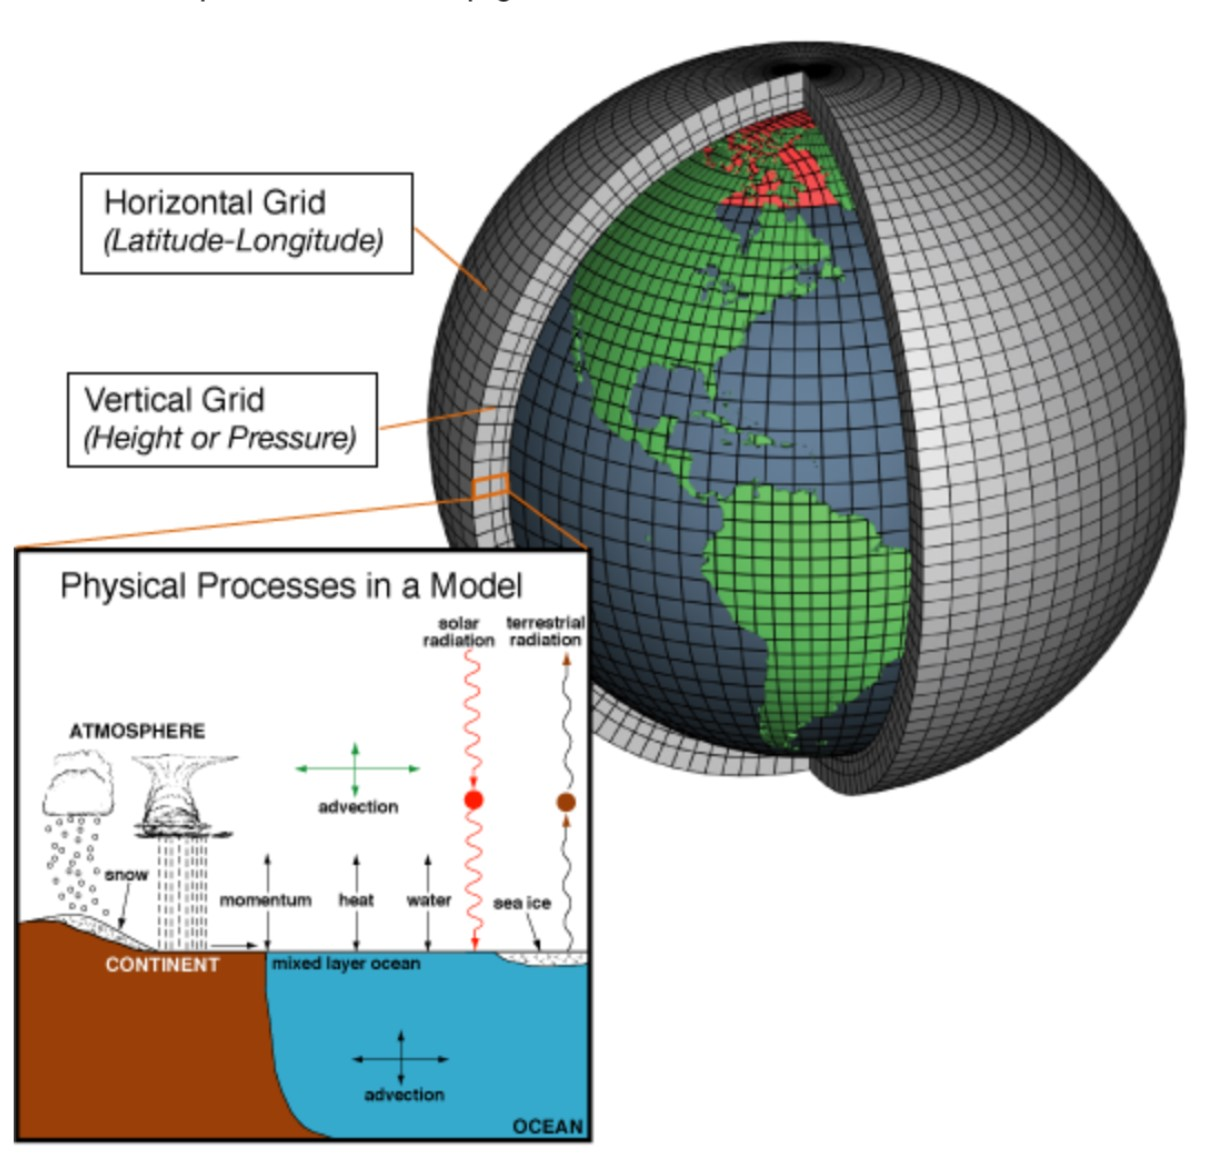
\includegraphics[width=8cm,height=24cm,keepaspectratio]{images/tropical-cyclones/climatemodel.jpg}
\caption{}
\label{fig:figure 6}
\end{figure}

When a model is “run”,\red{we can move this the the climate change chapter if you would like and then just summarize the topic as it relates to your chapter, might be less repetitive for the reader and we'll add you to another chapter authorship} scientists set the variables to certain predictable climate conditions, such as greenhouse gas concentration, and solve the equations for those conditions \citep{noaaclimate.gov}. The results are then plugged into the next grid, and so on, representing the passage of time. To test the models, climatologists run the models back in time, ensuring the results are similar to what has actually been observed before simulating future conditions.

\red{back to your topic, right?}
Applied to tropical cyclones and climate change, these models allow scientists to make conclusions about how greenhouse gasses will affect storms. While the effects of climate change on storm frequency are unclear(\citep{emanuel2013downscaling}, \citep{chen2021typhoons}), multiple studies have shown an increase in tropical cyclone intensity due to climate change \citep{zhang2017response}, \citep{emanuel2013downscaling}, \citep{chen2021typhoons}. This finding is in consonance with what the physics of tropical storms predicted \citep{emanuel1987dependence}. Presented graphically, this can be seen by an increase in PDI in climate models set for expected greenhouse gas concentrations over the next century (recall that PDI is calculated using wind speed, one of the physical processes modeled in climate models). In sum, tropical cyclones can be modeled with the carnot cycle to predict the maximim power output of the storm. This model predicts that an increase in greenhouse gas concentration will cause storms to become more powerful, a prediction that is backed up by climate modeling.

\begin{figure}
\centering
\includegraphics[width=8cm,height=24cm,keepaspectratio]{images/tropical-cyclones/pdigraph.jpg}
\caption{}
\label{fig:figure 7}
\end{figure}

\red{GREAT chapter, I love the physics and discussion of carnot cycle, I think we might back up and teach some thermodynamics as another "interuption" into the history of the phillipines, I have some ideas of you want to think about it}


\chapter{Climate Infrastructure in Vietnam}

\section{Introductory}

How climate change will impact Vietnam

Flooding (especially coastal urban areas)

Sea Level Rise

Land Erosion

Health outcomes

Current Adaptation Plans

Strengthen existing barriers and infrastructure

Adapt cities expecting sea level rise

Withdraw from the coastlines in areas that are well below sea level

What's Needed for the Future

Stronger healthcare system

Support for farmers and agricultural workers

Support for rural population near Mekong and Red river deltas

\section{Conclusion}

Implications for other places in the region


\chapter{Coral Reefs, Ecosystem Services, and Indigenous Peoples}

\chapterauthor{David Chengwen Gorman}

\section{Coral Reef Ecosystem Functioning and Interactions}

\subsection{Coral Reefs: An Introduction\red{heading not capturing the content.}}

\red{title is asking the reader to know what ecosystems services are\ldots, you can either define or cite one of my chapters and I can add that text myself}

In November 2018, North Sentinel Island, an island in the Bay of Bengal smaller than 60 square kilometers, drew international attention after its indigenous inhabitants killed an American missionary. The Sentinelese, one of the last uncontacted people groups in the world, have occupied North Sentinel island for the last 60,000 years. Surrounded by shallow, razor-sharp reefs, the Sentinelese have managed to remain isolated from the rapid development of neighboring Southeast Asian countries and still practice traditional customs and ways of life \citep{Smith}.\red{a map of their location might be useful}

This hunter-gatherer tribe is just one of the thousands of Southeast Asian communities that rely on coral reefs for both protection and sustenance. While most do not practice the traditional hunter-gatherer harvesting practices of the Sentinelese, coral reefs remain fundamental to the lives of millions across Southeast Asia. Unfortunately, coral reefs face significant threats and at the current rate of degradation, reef survival is unlikely. The declining health, in terms of biodiversity, biomass, and fitness, of coral reefs impacts not only the overall condition of the global environment, but negatively affects the majority of the Southeast Asian population. Of these millions, marginalized groups like the indigenous peoples of Southeast Asia are affected disproportionately. Reef destruction will severely harm both the livelihoods and sovereignty of the Sentinelese and other groups like them. 

The coral reefs have become vital components of many Southeast Asian, coastal communities and indigenous groups alike. This fragile, colorful marine ecosystem boasts high levels of both biodiversity and biomass, which are vital to both reef survival as well as the millions worldwide dependent on reefs for sustainably and economic prosperity. These life sustaining ecosystems are akin to the rainforests of the sea. There are nearly 100,000 square-kilometers of coral reefs in Southeast Asia supporting between 600-800 different coral species. Healthy coral reef ecosystems provide various anthropological benefits, or ecosystem services, to people of all socioeconomic backgrounds. Reefs, with their high levels of biodiveristy and biomass, provide food to over a billion people annually, are a major destination for tourism, and hold great promise for biomedicine. 

As a multi-faceted and dynamic ecosystem, the reefs are constantly changing. They face countless threats and stressors, including the effects of climate change, pollution, and overfishing; the reefs are struggling. General reef health serves as an indicator for both global and marine ecosystem health, and unfortunately, the easily observed reef degradation is representative of many other ecosystems worldwide \citep{RAR}.

This chapter describes coral reef ecosystems and current environmental and anthropocentric threats to coral reefs in Southeast Asia.  Because of reefs high value to Earth and indigenous groups, conservation is essential; reef restoration efforts will also be highlighted. The following sections will detail the dynamics, threats, and benefits of the Southeastern Asian coral reefs, while focusing on indigenous interactions and their reef reliance. This chapter will stress the importance of reef protection and restoration, and how it is not only an ecological issue, but an environmental justice one as well.\red{could you add, after reading this chapter the reader should appreciate... three or so bullets -- these are like take home messages} 

\subsection{Coral Functioning\red{is this the best heading?}}

\red{is all this information needed by the reader? Can do these discriptions align with why they are vulnerable?}

Coral is composed of tiny animals referred to as polyps. Hundreds of thousands of these polyps work together to build the visible coral structures which comprise reef ecosystems. Each coral polyp uses calcium and carbonate ions that have been dissociated in the surrounding water to create calcium-carbonate (limestone)\red{limestone is a metamorphic rock, not sure you want to say this, but check on this} skeletons (Figure~\ref{fig:coralanatomy}). During the day, these vulnerable, nocturnal creatures \red{hide to } protect themselves by hiding in their limestone \red{?} skeletons. At night, they extend their \st{many}\red{give the number... but in a new sentance and} tentacles to feed, using specialized cells called nematocysts to stun their prey before consumption. These nematocysts are commonly observed on sea anemones, which makes sense, as coral polyps are part of the same, family Anthozoa.\red{revise} Most species of coral are extremely slow growing, and the majority grow by less than an inch every year \citep{coralreefalliance_2021}.\red{remind reader why this is important to your chapter}

\begin{figure}[h!]
\centering
\includegraphics[width=0.7\linewidth]{images/CoralAnatomy}
\caption{This simplified diagram illustrates the anatomy of each coral, its skeleton, and symbiotic zooxanthellae relationship. The mouth of each coral polyp is surrounded by tenacles, each full of stinging nematocyte cells. The zooxanthellae inhabit the tentacles, and, along the coral, use the limestone skeleton underneath for protection. Hundreds of thousands of these polyps compromise a single “\red{fix quote symbol}visible coral,” all working sharing the same calcium-carbonate skeleton \citep{noaa}.}
\label{fig:coralanatomy}
\end{figure}

The majority of corals, and the ones more essential for the contruction of the reef ecosystem, are classified as hard corals.\red{show images?} These corals are reef-building corals, or hermatypes. They create the calcium carbonate skeletons which support the coral reef ecosystem. The shape of these skeletons, while heavily influenced by genetic composition, is also largely dependent on the surrounding environmental conditions to which the coral is subject.\ref{be sure to tell the readers why this is important to the content of the chapter} In rougher water with stronger waves breaking over the reefs, hard corals tend to create a stronger, more robust stable shape, like a mound or coral flat. In contrast, corals in more sheltered, calmer waters can create complex shapes with intricate branching patterns \citep{coralreefalliance_2021}.  

The body of each coral is \red{actually--this word isn't all that effective in writing, unlike in talking, we all the time! Or, if you told us why this is so counter intuitive, then this would be more clear and you wouldn't need this word\ldots :-)} clear\red{how about transparent?}; the intricate colors come from single-celled eukaryotic cells called dinoflagellates, more commonly refered to as algae.\red{I thought these are noctornal and hide during the day\ldots going to need more info on this!} This grouping of small, photosynthetic algae live inside the coral skeletons and maintain a close, interactive relationship advantageous to both species reffered to as symbiosis. The algae symbiotes within the corals are generally referred to by their colloquial\red{why?}, zooxanthellae. \citep{noaa}. These algae grow inside the coral and photosynthesize, providing the necessary nutrients and oxygen the coral needs to grow and survive. The coral protects the zooxanthellae with its calcium-carbonate skeleton, and via respiration, provides the carbon-dioxide needed for photosynthesis. This symbiotic relationship between coral and algae is delicately balanced, and small disruptions can have catastrophic effects not only for the organisms involved, but also for the entire ecosystem as a whole. \citep{https://doi.org/10.1002/fee.2088}  

Corals are incredibly\red{relative term that probably can't be understood by most readers} slow growing, as they require a delicate balance of nutrients and environmental conditions. Both nutrient influxes and nutrient deficiencies interrupt the coral-zooxanthellae symbiosis, hurting both species. Most species only grow between 0.2-1 inch per year. A reason for this slow growth is that coral reproduction mechanisms are easily disrupted, either from localized pollutants or globalized climate change related issues.\red{cut by 25\%, let's see if we can be more effecient}  

All coral reproductive processes are affected by the water temperature, time of the year, tidal cycles, and lunar cycles, and they vary by species.\blue{good, thus vulnerable to changes!} \red{Does this later discussion help link in our understanding of their vulnerability? I believe so, but only if mentioned later do you want to keep each\ldots} Some coral species are hermaphrodites, able to produce both eggs and sperm at the same time. Others are gonochoric and can only produce one of the two gametes. Coral larvae can be formed either inside the polyp body or outside the polyp body, such as during mass gamete ejection events. Coral larvae are released into the water, where they are free swimmers. They first swim to the surface, and then fall back to the seafloor where they must attach to a hard surface, like a rock or preexisting coral skeleton. This hard surface provides the polyps with a sturdy base and protection, and the corals can begin dividing and making genetic copies of themselves. They then can begin secreting the calcium carbonate skeleton, which in turn attracts zooxanthellae seeking protection, and the symbiotic relationship begins \citep{coralreefalliance_2021}.

For the duration of this chapter, the term ``coral'' will be used to describe the network of polyps which comprise the visual structures of the reefs. 

\subsection{Reef Organisms and Trophic Interactions}

The coral reef food web (Figure~\ref{fig:ExampleReefFoodWeb}), or the relationship between successive trophic levels of the community, starts as any other food web, with energy being derived from the sun by primary producers via photosynthesis. These primary producers include seaweed, grass, phytoplankton, and perhaps most importantly, the zooxanthellae coral symbiotes. This\red{avoid pronouns} is the largest group, as only about 10\% of the energy in each trophic level is passed to each successive level. The second trophic levels, the primary consumers, includes zooplankton, mollusks, squirrelfish, urchins, and of course, the coral polyps themselves. Following this are the secondary consumers, made up of triggerfish, Parrotfish, butterfly fish, and more. Finally, tertiary consumers like the reef shark and barracuda finish this food web, with detritivores like sea cucumbers or bacteria decomposing and recycling organic matter back into the ecosystem \citep{https://doi.org/10.1890/15-1492.1}.

\begin{figure}[h!]
\centering
\includegraphics[width=0.75\linewidth]{images/reeffoodweb}
\caption{Food webs like the one displayed above illustrate the many different feeding interactions within the reef ecosystem. No food web can be completely comprehensive, as the reefs are home to thousands of different species, all interacting with each other. Species may fall into multiple trophic levels depending on their diet and feeding interactions. Food webs like the one shown above provide simplified examples of the feeding relationships and energy transfers within the ecosystem.\citep{https://doi.org/10.1890/15-1492.1}.}
\label{fig:ExampleReefFoodWeb}
\end{figure}

A wide range of species in the reef ecosystem depends on coral polyps, thus making them a keystone species. As ecosystem engineers\red{are they both? confusing to use both terms interchangeably}, they provide the entire structure and habitat from many reef-dwelling creatures with their calcium carbonate skeletons. The coral polyps themselves constitute a small percentage of the total biomass of the ecosystem, as the average coral polyp is only around 1.5 cm large, yet their impact is vital to the ecosystem's survival. To the naked eye, observable ``coral’’\red{should be two single quotes} includes these skeletons, and the symbiotic algae living within them; the coral polyps themselves make up a significantly smaller biomass percentage as one would perceive. 

Many species depend on these coral skeletons for either protection or as hunting grounds. Fish, invertebrate, and other organisms aggregate around these underwater structures, accounting for the ecosystem\red{’}s dense biodiversity and high overall biomass. Some argue that the Parrotfish is another, secondary keystone species. This herbivorous fish eats algae latched onto the coral skeletons, which blocks sunlight and limits the photosynthetic abilities of the zooxanthellae. In a sense, its mutualistic niche is to ``clean the coral,'' allowing normal function to continue. The Parrotfish is a highly targeted, overfished species, and because it fulfils an important niche, its removal negatively effects the entire reef ecosystem. This specific niche is just one of many, all which illustrate the complex relationships involved in the coral reef ecosystem and the importance of each species to the ecosystem \citep{https://doi.org/10.1890/15-1492.1}. 

\red{balances -- on paper this sounds great, but how is this measured?}

\begin{figure}[h!]
\centering
\includegraphics[width=\linewidth]{images/urchin}
\caption{:Pictured above is a seafloor that has been completely overrun by urchins and cannot effectively sustain life anymore. As anthropologic activities influence organism within ecosystems, the natural checks and balances systems degrade and certain species may quickly become dominant, seen with the urchins and the creation of these urchin barrens. The simple removal of the urchin\red{’}s keystone predator, the orange-lined triggerfish, can be enough to cripple entire ecosystems, illustrating the fragile balances within the reef ecosystem \citep{https://doi.org/10.1890/15-1492.1}. }
\label{fig:UrchinBarrenExpanseoveraDyingReef}
\end{figure}

These inter-organism \red{we usually write, inter-speices} relationships can be further illustrated by an examination of the indirect actions which affect entire ecosystems and stem from trophic-level suppression, known as trophic cascades. For Southeast Asian reefs, the most prolific trophic cascade exists between urchins and the orange-lined triggerfish. The triggerfish is a keystone predator and limits uncontrolled urchin expansion. Without these predators, urchin populations would explode and consume everything on the seafloor, creating urchin barrens (Figure~\ref{fig:UrchinBarrenExpanseoveraDyingReef}) incapable of supporting life.These predator-prey interactions are disrupted by anthropocentric activities, mainly overfishing. As the fish are removed from the ecosystem at an unsustainable rate, the detrimental grazer effects of the urchins are exacerbated. While negative human influences will be discussed in future sections, this illustrates how interconnected reef species are the delicate equilibrium between them\blue{great connection} \citep{https://doi.org/10.1890/15-1492.1}.

\subsection{Necessary Climate and Nutrients}

Coral reefs require a delicate balance of nutrients and external conditions, which is easily disturbed, making them especially vulnerable. As for physical needs, sunlight is a crucial limiting factor of the ecosystem. The zooxanthellae require shallow waters with low turbidity, or high clarity. This means they generally can only survive in waters under 50 meters, mostly free of sediment and debris. The water also cannot have too many nutrients, as rapid, uncontrollable, explosive algae growth can cloud waters and block the necessary sunlight needed for photosynthesis\red{define what you mean by this--in particular, what are the concentatons of concern?}. Corals reefs exist in tropical climates usually, as they also need warmer waters of around 20-32 \degree C (68-90 \degree F). Finally, corals need water with a high salinity, or saltwater concentration. They cannot survive in brackish water or estuaries, or anywhere where freshwater sources like rivers drain into the ocean. The tropical, warm climate of Southeast Asia satisfies the aforementioned necessary reef-building conditions, explaining the abundance of coral reefs in the region \citep{https://doi.org/10.1002/fee.2088}.

\begin{figure}[h!]
\centering
\includegraphics[width=0.70\linewidth]{images/reefcycles}
\caption{The above cycles and reciprocal processes are vital for coral growth and survival.They will be further discussed in the following paragraph. Figure from: \citep{https://doi.org/10.1002/fee.2088}. } 
\label{fig:ReefEcosystemFunctioningandIntrisnsicDrivers}
\end{figure}


The first, blue cycle (Figure~\ref{fig:ReefEcosystemFunctioningandIntrisnsicDrivers}), calcium carbonate dynamics, is directly correlated with the coral skeleton formation. Bioerosion, or the breakdown of hard oceanic substrates, leaves behind calcium and carbonate ions, which coral polyps use to produce their limestone skeletons. The second, green cycle (Figure~\ref{fig:ReefEcosystemFunctioningandIntrisnsicDrivers}), herbivore-algae interactions, involves both primary production and herbivory. Photosynthetic organisms transform sunlight into chemical energy, which is then moved up in trophic levels by herbivores. A balance between the two must be maintained to prevent explosive growth of lower trophic levels, which in turn could suppress crucial processes carried out by other organisms in the ecosystem\red{need to be more precise}. Predator-prey interactions, the orange cycle (Figure~\ref{fig:ReefEcosystemFunctioningandIntrisnsicDrivers}), also regulate explosive trophic level growth, as successive trophic level limits the prior. Again, the balance keeps the biomass of one species from dominating and smothering other species. The final process driving success within the coral reef ecosystem is the purple cycle (Figure~\ref{fig:ReefEcosystemFunctioningandIntrisnsicDrivers}), nutrient cycling, or the uptake and release of nutrients among the organisms of the ecosystem. Nutrients must be moved efficiently and effectively in cycles\red{avague in terms of what that actually means}, with a balance\red{define} maintained between retention and reintegration \citep{https://doi.org/10.1002/fee.2088}.

\subsection{Southeast Asian Reefs by Country}

\blue{let's see if we can cut the word count}

\red{Although c}Coral reef locations are relatively limited, \red{they can be found\ldots}, as the previously mentioned conditions must be satisfied, yet they\red{occur} can be found in over 100 countries, mainly between the Tropics of Cancer and Capricorn. Many reefs are concentrated in shallow waters surrounding islands of the Indo-Pacific. Reefs surrounding both Indonesia and the Philippines compose a majority of not only Southeast Asian reefs, but also reefs worldwide (Figure~\ref{fig:MapofSoutheastAsianCoralReefs}).\red{see if you can cut in 1/2} Coral reefs cover 284,300 \red{\kms} square kilometers (110,000 square miles) worldwide, yet the overall area of healthy reef is decreasing rapidly \citep{Watlas}.

\begin{figure}[h!]
\centering
\includegraphics[width=0.6\linewidth]{images/reefmap}
\caption{This map not only shows the locations of Southeast Asian coral reefs, but also the relative risk levels associated with each reef. The threat levels are as follows: blue = low, yellow=medium, red=high, maroon=very high. The suggested threat levels describe local threats; global threats like climate change are not accounted for \citep{Watlas}.}
\label{fig:MapofSoutheastAsianCoralReefs}
\end{figure}

\begin{table}[h!]
\caption{Southeast Asian Coral Reef Size by Country \red{ label needs to be one word or hyphonated pharse to work}. \blue{also, I changed to right justified in table, better?}}
\label{tab:Southeast-Asian-Coral-Reef-Size-by-Country}
\begin{tabular}{lrrr}
Country     & \st{World Reef Area }Rank\st{ing} & Reef Area (\red{\kms}) & Percentage of World Total Reef Area\st{ (\%)} \\ 
\hline\hline
Indonesia   & 1                       & 51,020            & 17.95\% \\ 
\hline
Philippines & 3                       & 25,060            & 8.81\%  \\ 
\hline
Malaysia    & 17                      & 3,600             & 1.27\%  \\ 
\hline
Japan       & 23                      & 2,900             & 1.02\%  \\ 
\hline
Thailand    & 26                      & 2,130             & 0.75\%  \\ 
\hline
Myanmar     & 27                      & 1,870             & 0.66\%  \\
\end{tabular}
\end{table}

\st{Listed are some notable} Southeast Asian countries \blue{have a disproportional area of reefs ??} Table\ref{tab:Southeast-Asian-Coral-Reef-Size-by-Country} and their respective reef areas. While Indonesia and the Philippines dominate total reef area, many coastal Southeast Asian countries have reefs of their own, all which face similar anthropologic pressures. Reefs are spread Southeast Asia accounts for over a quarter of all the worlds coral reefs \citep{Watlas}.\red{cut by 20\%}

\section{Climate Change and Its Effects on Coral Reefs}

\subsection{The Indigenous Paradox}

\blue{takes too long to hear what the indigenous paradox is\ldots, maybe add a subsection on impacts of warming?}

Climate change and global warming are undoubtedly one of the biggest contributors to the loss of biodiversity and overall destruction of coral reefs\red{why?}. \blue{needs better transition}The IUCN Red List Index (RLI), a comprehensive list tracking biodiversity loss and extinction risk, identifies corals as one of the fastest declining species (in terms of diversity and richness) in response to climate change \citep{wwfindex}. Even \blue{if?} all localized reef threats and pollutants were eliminated, the overarching threats of ocean acidification and rising temperatures \red{hold the ability--wordy} to eradicate reefs entirely \citep{Keller2009ClimateCC}.\blue{cut by 30\%}

In addition to reef eradication, climate change disproportionately effects lower socioeconomic classes, specifically, indigenous people groups. Many Southeast Asian indigenous coastal peoples are reliant on reefs not only for food and sustenance, but they also have strong cultural ties to the reefs and surrounding waters. Climate change threatens these indigenous people-reef ecosystem interactions, and these threats compound other climate change-associated dangers affecting indigenous groups. As many indigenous groups inhabit harsh and isolated environments, they are highly vulnerable to the rising sea levels and increased storm severity resulting from climate change. They are also often excluded from policy discussions and legislative responses to climate change, further increasing their susceptibility to climate change disturbances \citep{13772149520190801}.\blue{you talk about this earlier and later right?  Feels like this isn't concrete enough to repeat unless you give examples}

\red{first sentence to describe term\ldots at the top of the subsection} Oddly, indigenous groups are some of the most well-adapted and resilient groups in response to climate change as well. Knowledge of specific environments and ecosystems is passed down generationally, creating a plethora of knowledge concerning responses to environmental issues, all which can be used to combat the effects of climate change. This ecosystem expertise and resilience, coupled with their high vulnerability to climate change, creates what some call ``The Indigenous Paradox.'' Indigenous groups all throughout Southeast Asia are continually ransacked by reef degradation in response to climate change, yet their complex, generational knowledge is vital in combatting climate change and reversing its current narrative. Indigenous peoples offer highly valuable resources concerning reef restoration, which will be discussed further in Section \ref{sub:ie} \citep{13772149520190801}.\blue{re-arrange of cut by 30\%}

\subsection{Rising Sea Level}

A primary issue when discussing climate change and the ocean is rising sea levels. This is due to both melting polar ice caps and thermal expansion of water molecules caused by the rapid increase in temperature, or thermal heat, in recent years. Sea levels are projected to continue to rise 0.5-1.5 meters by 2100, undoubtedly impacting both submerged ecosystems and coastlines worldwide. \citep{coralreefalliance_2021}.\red{not the primary source -- needs to be an author of authority}

\blue{In contrast to the negative impacts,} Brian Keller, Regional Science Coordinator of NOAA's Office National Marine Sanctuaries, and his colleagues conducted a study concerning sea level rise and its effect on corals on the Sanya Bay of the South China Sea, where they discovered a potentially unforeseen positive development: the sea level rise promoted coral growth. The previously degraded reef was able to recolonize via asexual fragmentation in response to the 16.2 $\Mypm$ 0.6 cm rise over the previous 30 years. Of the corals the study surveyed, 86\% were under 30 years old, suggesting that the rise in sea level promoted their growth. This phenomenon can be explained by the rise in coral growth accommodation space, as sea level rise increases the vertical space a coral can grow in. As the coral gets closer to the surface, growth is inhibited by temperature, exposure, and sediment, but by increasing the overall depth, growth can occur in a greater area of water. At first glance, this promising result suggests that climate change actually may benefit coral reefs in some way, but that is unfortunately not the case. Only specific coral species are suited for a rapid rise in accommodation space, which may select out other species. This leads to an increase in total growth but a decrease in biodiversity, and with organisms as vulnerable as coral, biodiversity is crucial \citep{sealevelrise}. Retrospective studies have also found that coral growth rates increased with sea level rise over 16,000 years ago, and then faltered as the sea level became stabilized during the Holocene (current time period, which began 11,700 years ago), but these results cannot be taken as indications of future outcomes. Coral growth capacity is likely to be inhibited by other factors, both regional and global, so an increase in accommodation space may have negligible overall impact \citep{Keller2009ClimateCC}.\blue{nice, see if you can but by 30\%}

The negative effects of sea level rise on the coral reef ecosystem are relatively unquantified, yet practically accepted as true based on past events and prospective insight. As sea levels continue to to rise, they pose risks to coastal regions, with the threat of washing entire communities into the ocean.  Such catastrophic events would undoubtedly add sediment and pollutants to the water while also physically damaging corals and other organisms with the marine debris. Community submergence would also displace people groups, causing them to either move inland or to other coastal areas. Many would likely move to other coastal areas to practice similar lifestyles, which would in turn concentrate pressure on reefs not yet affected by coastline degradation. The increases storm surge and flooding associated with climate change will most strongly contribute to coastal retreatment. Already, over a million people in over 27 places worldwide have been forced to retreat inward, and this number will only increase incrementally as climate change continues to worsen. \citep{Sinay_2020} Indigenous groups and other coastal communities are disproportionately threatened by sea level rise, as the already underrepresented groups will be forced off their land now not only by oppressive governments and corporations, but also by nature itself. As rising sea levels and issues of displacement increase, even benevolent governments struggle to accommodate affected citizens and displaced people groups. These threats to coral reefs may seem distant, but they are quickly approaching realities imposed by climate change \citep{Keller2009ClimateCC}.\blue{nices, see if you cut 20\%}

\subsection{Ocean Warming and Acidification}

Climate change has already begun to negatively impact reefs in quantifiable ways that can be observed at the molecular level.As greenhouse gases are released and trapped in the atmosphere, they prevent heat escape and also contribute to smog and air pollution. The primary greenhouse gas, carbon dioxide (\carbondioxide), is released in high amounts when fossil fuels like coal and natural gases are burned for energy. Fossil fuel emissions release carbon dioxide into the atmosphere, but \blue{scietists believe\ldots} about one third of the \carbondioxide is absorbed by the ocean. The increase in greenhouse gases emissions from fossil fuel burning contributes to both the warming of the planet and the acidification of the ocean\citep{Keller2009ClimateCC}, \red{while reducing the warming poenial\ldots no?} 

As atmosphereic carbon dioxide dissolves in the ocean, it reacts with water to create carbonic acid. This carbonic acid then dissociates into bicarbonate, releasing protons in the process.These protons, when added to the water, lower the pH, making it more acidic (Figure~\ref{fig:OceanAcidifcationChemicalReactionandItsCarbonateRelation}). Since the Industrial Revolution, a 0.1 pH drop has been observed on the ocean surface, and this drop is expected to increase as global emissions continue and \carbondioxide concentrations rise. In more acidic conditions, corals struggle to efficiently create their hard skeletons \citep{Keller2009ClimateCC}. The carbonate ion saturation, or aragonite saturation, is crucial for skeletal growth, as the carbonate ion is one of the two necessary ingredients needed for limestone\red{wrong word, I think} formation. The bicarbonate ion formed by the carbonic acid-carbonate interactions is unusable to corals, thus slowing skeletal growth (see figure for complete chemical process) \red{Figure~\ref{fig:OceanAcidifcationChemicalReactionandItsCarbonateRelation}} Today, up to 60\% of reefs persist in waters with inadequate\red{what does this mean? what concentration should they by?} aragonite saturations \citep{Ayala_2009}.

\begin{figure}[h!]
\centering
\includegraphics[width=\linewidth]{images/acidification2_med}
\caption{The above figure outlines the chemical reactions which connect ocean acidification with limestone formation. As carbon dioxide dissociates in the water, it creates carbonic acid, or H$_2$CO$_3$. The protons of carbonic acid are easily dissociated by the more polar water molecule (H$_2$O), thus dissociating and combining to form bicarbonate, or HCO$_3$. The dissociated protons may also form bicarbonate by reacting with carbonate ions. This chemical reaction removes carbonate ions from the water, which corals need to construct their calcium carbonate skeletons  \citep{Ayala_2009}.}
\label{fig:OceanAcidifcationChemicalReactionandItsCarbonateRelation}
\end{figure}

The skeletons built by corals in waters lacking proper carbonate ion concentrations not only form slower but are also weaker and less robust\red{meaning?}. As a result, corals have fewer defenses to fight pressures and, combined with the slowed growth rates, may not be able to overcome the pre-existing stressors they face. Increasing acidification will likely cause coral production rates to fall below destruction rates, decreasing reef size and affecting the ecosystem as a whole. Additional stress from acidification and climate change only adds more threats to coral, creating a detrimental positive feedback loop for the already struggling polyps. The effects of ocean acidification compound on each other. The weaker skeletons stemming from low carbonate ion concentrations cannot adequately protect the corals, resulting in even lower skeletal production and exacerbating the preexisting consequences of ocean acidification on corals. 
 \citep{Ayala_2009}.

On top of \red{what does this phrase imply? physical relation, which isn't accurate}ocean acidification, as greenhouse gas emissions continue to cause earth's surface to warm, the ocean warms with it. This rise in temperature is the main cause of sea level rise, due to both glacial melt and the molecular expansion of water molecules in response to heat. Ocean warming and its effects on coral reefs is still a topic requiring more research, but its effects have already begun to be observed \citep{wwfindex}. \ref{author of authority?}

Coral disease transmission is exacerbated by higher temperatures, which will be explored further in Section \ref{sub:cd}. Unusually high-water temperatures are the main cause of coral bleaching, and as ocean temperatures continue to rise, mass bleaching events are expected to increase in both frequency and severity\citep{Keller2009ClimateCC}. Ocean warming will have disastrous future effects on coral reefs.  In 2018, Intergovernmental Panel for Climate Change, or IPCC, reported that a mere two-degree Celsius rise in temperature could completely eradicate the coral reefs, with an estimated loss of around 99\% of reefs worldwide \citep{wwfindex}. \red{author of authority?}

\subsection{Coral Bleaching}

Coral polyps react to warming water temperatures and other environmental stressors by expelling their algae. If the waters do not cool or the stressor continues to persist, the algae will not come back, and the coral will starve without them. The starved corals crumble into empty, white, lifeless skeletons. Both species are interdependent and persist in close proximity to each other . They maintain an obligate mutualistic relationship; they cannot survive without each other. The expelling of algae symbiotes in response to different stressors is known as coral bleaching (Figure~\ref{fig:CoralBleaching}), and it has the potential to destroy entire reef ecosystems in an alarmingly short period of time \citep{https://doi.org/10.1111/gcb.14871}.\red{good stuff, can you reduce by 25\%, it's a bit wordy.}

Most bleaching and mass coral mortality events are driven by heat waves, which have increased with climate change and global warming. The disruption of the coral-algae symbiosis caused by the loss of algal endosymbionts is what causes the corals to pale, as the algae are responsible for coral coloring. Without their symbiotes, the corals lose the ability to feed and rapidly starve and die off. Not only does this halt further reef growth, but this depletion of a singular species shifts the organismal balance of the entire ecosystem. These negative ecological cascades descend throughout the ecosystem. Many organisms' habitats are destroyed as the coral, the keystone species and ecosystem engineers, are removed. The population balances within the ecosystem in turn shift, for the species more directly dependent on corals are disproportionately affected by the bleaching events \citep{https://doi.org/10.1111/gcb.14871}.\red{reduce by 50\%}

\begin{figure}[h!]
\centering
\includegraphics[width=0.6\linewidth]{images/coralbleach}
\caption{This above split-image shows the same fire coral before (left) and after (right) coral bleaching has occurred. The vibrant colors on the left image result from the zooxanthellae symbiotes, and when the corals expel them, the ghostly white color seen on the right image is observed. This color change is universal across all coral species; only the color of the calcium carbonate skeleton remains after the algae are expelled \citep{https://doi.org/10.1111/gcb.14871}.}
\label{fig:CoralBleaching}
\end{figure}

Coral bleaching is the net outcome of complex, multifactorial stressors working at both the cellular and ecosystem levels. 

\blue{maybe?}
\begin{description}
\item[Cellular level] \st{accumulation of} reactive oxygen species, or ROS, accumulates and triggers signaling cascades prompting corals to expel their zooxanthellae. These ROS are both produced and accumulated in response to environmental changes and stressors. 
\item[Ecosystem\st{ and environmental} \red{landscape? oceanscape?} level], the most common stressor is heat waves. The first-ever observed mass coral bleaching event in 1998 was driven by El Ni\~{n}o, and rising temperatures have been accredited with the increasing frequency of bleaching events. The two recent back-to-back bleaching events in both 2016 and 2017 gained national attention, showing the vulnerability of the coral ecosystem to change on a global scale. These events also demonstrated how climate change will only make coral bleaching more frequent and of greater severity.
\end{description}

Other environmental exacerbators include, but are not limited to, light availability, salinity, oxygen demand, organic nutrient availability, and inorganic nutrient availability. 

While one of these single factors may not cause a mass bleaching event, they are interconnected and have cumulative effects on the fragile, not-easily-adaptable coral polyps. Each factor also can change how well coral adapts to rapid heat change. Coral bleaching is the result of a complex, dynamic system that global warming negatively affects in multiple ways \citep{https://doi.org/10.1111/gcb.14871}.\red{great stuff -- but can you reduce by 35\% with more succinct language?}

\section{Unsustainable Fishing Practices}

\subsection{The Live Reef Fish Trade}

\blue{discuss/define what you mean by fishing then unsustainable\ldots}
Unsustainable fishing practices are arguably the most detrimental local practice to Southeast Asian reefs. Over 55\% of reefs worldwide are affected by overfishing and unsustainable fishing techniques, and this number is higher in Southeast Asian reefs. Overfishing disrupts trophic interactions, since macroalgae, without as many fish as predators, grow disproportionality and smother corals. An overfishing-driven decline in fish stocks has made fish harder to catch, leading to a shift away from sustainable fishing practices. Unsustainable fishing threatens not only fish stocks and ecosystems, but also local economies and the people that rely on fish for food. The methods currently used to catch live fish, like cyanide fishing or blast fishing, have been incredibly destructive to the coral reefs of Southeastern Asia. Both Indonesia and the Philippines offer textbook examples of unsustainable practices which still persist today, despite efforts to regulate and ban them \citep{coralreefalliance_2021}.\red{needs better source}

A major driver of unsustainable fishing practices is the Live Reef Fish Trade, or LRFT, which is precisely as it sounds: selective fish are caught, kept alive, and later sold. There are two branches of the LRFT: food and ornamental. For the live food fish trade, these live fish are caught and sold as high-priced delicacies. The food trade makes up a majority of the LRFT, as has been continually driven by wealthy Asian countries' affinity for fresh, live fish. Certain high-commodity fish, like leopard coral reef fish, are targeted and fished for disproportionately, selectively pressuring reef ecosystems and disrupting trophic interactions. These fish can sell for as much as \$60 USD per kg instead of the average \$2 USD per kg for most fish. In locales such as Palawan, Philippines, where the average monthly income is under \$100 USD, it is no surprise the LRFT would flourish. Fishermen explain,``It's like hitting the jackpot every time.'' The second branch, the ornamental live fish trade, involves the catching of live fish for sale and transport to aquariums worldwide. The vibrant, colorful reef fish are highly desired in aquariums globally, sustaining demand and further fueling the LRFT. \citep{10.2307/40603032}. \blue{cut by 25\%}

Many of the practices for catching live fish are inherently destructive.\red{to what?} Fish are often caught young and then grown to an edible size. This excessive juvenile capture removes fish before they can reproduce and contribute back to the ecosystem, further reducing the fish stocks of the selected species. Other more violent methods, like cyanide and blast fishing, have horrid effects on reefs, and these will be discussed in the following sections \citep{10.2307/40603032}. 

The LRFT has continued to grow in both the Philippines and Indonesia despite both decreasing profitability and fish stocks. This dangerous combination has led to high levels of overfishing that further destroyed coral reefs. Fishermen are catching less fish and must travel farther distances to find them, causing large scale economic losses in both coastal communities and the individuals residing in them. Because the LRFT is poorly regulated and any existing regulations are often not enforced or disregarded, the harmful impact of the LRFT is likely to continue \citep{10.2307/40603032}.

\subsection{Cyanide and Blast Fishing}

The selective catching of live fish is easily accomplished through the use of sodium cyanide, which stuns larger fish to be later revived. While it may sound complex, cyanide fishing is as simple as diving with a spray bottle containing crushed sodium cyanide tablets which can be injected into reef crevices or squirted directly into the faces of desired fish (Figure~\ref{fig:CyanideFishing}). While larger animals may only be stunned and can later revive, smaller organisms are severely poisoned by the cyanide, as it represents a much larger proportion of their body weight and size.\red{wordy} These animals inevitably die, disrupting ecosystem functioning on multiple levels. Cyanide is most often fatal to small fish, invertebrates, corals, and their symbiotic algae \citep{wwfcyanide}.

	After just 30 seconds of cyanide exposure, coral becomes stressed and begins to lose its ability to function normally. For every live fish caught with cyanide, a square meter of reef is destroyed. Cyanide fishing is not only used for the LRFT, but also for aquarium trade as well. At the turn of the century, 75\% of all aquarium fish coming from Southeast Asia were estimated to be cyanide-caught. Around two-thirds of all Filipino reefs are estimated to be affected in some way by cyanide poisoning \citep{970313024119970301}.

Despite being banned in both Indonesia and the Philippines, cyanide fishing still persists today. Asia's growing affinity for live fish, with neighboring countries like China and Hong Kong making up the majority of the market, fuels the continued use of cyanide fishing. The Padilla region in the Philippines is responsible for around two-thirds of all live fish exports, exporting up to a ton of fish per day. Many of these live fish are caught via cyanide fishing. The minimal regulations and negligible punishments for cyanide fishing enable this destructive practice to continue. In the last six years, only six case files regarding cyanide fishing have resulting in 
convictions \citep{wwfcyanide}.\blue{cut section by 40\%}

\begin{figure}[h!]
\centering
\includegraphics[width=0.7\linewidth]{images/cyanidefishing}
\caption{The diver in this picture is cyanide fishing in a Filipino reef. He uses cheap, makeshift gear which can be either made from scrap or repurposed. The warm, coastal waters allow him to dive without a wetsuit, only using wood planks nailed to slippers as fins. His bottle contains crushed sodium cyanide tablets dissolved in water, a lethal solution which will decimate the reef he is injecting it into \citep{wwfcyanide}.}
\label{fig:CyanideFishing}
\end{figure}

Blast fishing is another way to stun fish for the live trade harvest. Explosives are detonated in reefs to stun fish, which are then selectively chosen for live trade. Like cyanide fishing, smaller organisms are often immediately killed by these blasts, and the coral is as well. Because blasts also break the preexisting coral skeletons, both the habitat and entire ecosystem are destroyed. Over half of all Southeastern reefs are threatened by blast fishing practices \citep{https://doi.org/10.1890/1051-0761(2006)016[1631:RFBFOC]2.0.CO;2}. 
  
The explosives used are almost always homemade and can be as simple as a kerosene-fertilizer mixture inside a glass soda bottle. Just one 300mL bottle can create an explosion which leaves behind a crater with a 1-meter radius capable of lasting multiple years. Besides the general fatalities from the blasts, one of the biggest issues associated with blast fishing is the leftover coral skeleton debris. An examination of craters left behind by blast fishing concluded that even after five years, the rubble and debris left inside the crater was between 5-10 cm deep. This additional sediment can smother both coral and algae, either blocking light and hindering photosynthesis or burning still-intact corals alive. Larger debris and skeletal pieces can also abrase growing corals, scraping off growing colonies or hindering recruitment by blocking secure surfaces for attachment \citep{https://doi.org/10.1890/1051-0761(2006)016[1631:RFBFOC]2.0.CO;2}. 

Over half of all Southeast Asian reefs are currently threatened by blast fishing practices. Again, like cyanide fishing, blast fishing is legislatively banned, but this ban is barely enforced. Blast fishing was banned in Indonesia in 1985, yet it still continues today, not only in Indonesia, but also in most other reef-bearing Southeastern countries \citep{https://doi.org/10.1890/1051-0761(2006)016[1631:RFBFOC]2.0.CO;2}. 

\blue{cut section by 40\%}

\subsection{Economic Drivers and Indigenous Contributions}

A group of indigenous peoples deeply interconnected and dependent upon unsustainable reef fishing is the semi-nomadic, boat dwelling communities of Southeast Asia. These maritime communities are reliant on the sea for subsistence, often inhabiting areas of high biomass and biodiversity, as resources are often concentrated there. As a result, many of these communities are situated near coral reefs and rely on them; to them, reef survival means human survival \citep{boatpeople}. 
One of these groups, the Sama-Bajau, reside mainly in the Philippines and eastern Indonesia. Foods derived from reefs provide a majority of their protein intake, and fishing is a dominant economic sector among the group. Most other economic activities among the Sama-Bajau relate to reefs, as reef reliance supports a wide range of activities, from boat building, to guiding tours, to sea trading. Many groups like the Sama-Bajau have modernized to incorporate stilt houses, giving them more of a sense of community and stability. Unfortunately, many other groups are not officially recognized and lack legal representation, and in turn cannot officially own land areas for settlement. The resulting highly mobile lifestyle deprives these groups of not just landownership, but also healthcare, education, and traditional economic prosperity \citep{boatpeople}.\blue{nicely documented}

Because of the many factors contributing to indigenous suppression and poor socioeconomic conditions, the vast majority of the reef fishermen are poor and struggle to sustain themselves and their families through traditional fishing practices. One factor of interest is the drop-out rates among children in these indigenous groups. The reef-reliant, seafaring lifestyle is commonly not respected among upper socioeconomic classes, for these indigenous groups are viewed as primitive and uncivilized. As a result, indigenous children face widespread racial and cultural discrimination, leading them to drop out of school and pursue a less economically prosperous career, like fishing. As reefs are continually degraded by overarching issues, such as climate change and local issues (e.g., corporate overfishing and pollution), sustainable fishing practices become less viable. Many Sama-Bajau fishermen, like other indigenous fishermen, have turned to the more lucrative unsustainable fishing practices like blast fishing and cyanide fishing. Driven by the high demand of the LRFT and aquarium trade as well, these destructive fishing practices promise steady, higher payouts than traditional fishing methods. Indigenous participation in these activities is not driven by economic greed, but purely because they lack other alternatives to feed their families. These fishing practices further degrade reefs, putting indigenous groups in a viscous cycle of reef degradation and economic activity loss. The drivers of many of the previously mentioned unsustainable fishing practices result from a complex system of oppression, especially among indigenous groups of Southeast Asia \citep{boatpeople}.

\blue{see if you can cut section above by 10\%}
\section{Reefs Pollutants}

\subsection{Marine Debris and Ocean Contaminants} \label{sub:mdoc}

A significant number of anthropocentric activities contribute to reef pollution. Pollutants can be classified generally in three categories: toxins, sediments, and nutrients. Toxins cause physical harm to corals and other organisms at the cellular level. They can be organic or inorganic and are often found in chemical runoff. Sediments block sunlight and prevent photosynthesis and limit primary production. They also reduce the number of viable locations for coral larvae to attach to, as the loose sediment settles on the previously secure spots on the coral skeleton. Sediment also increases the turbidity of the water, blocking visibility. This can contribute to biodiversity loss, selecting for certain animals which do not primarily rely on eyesight. Finally, nutrients can promote algal blooms which smother corals, or they can disturb organismal balances within the ecosystem, disrupting critical interactions among populations. Excessive nutrient richness, or eutrophication, can also promote pathogenic growth among corals and lead to coral epidemics. A wide range of human activities contribute to reef pollution, with globalization, population expansion, and development as main exacerbators \citep{4884777420100401}.

Marine debris is essentially human trash, which enters the water via boats or from land. (Figure~\ref{fig:marinetrash}). Floating trash can bear resemblance to jellyfish and is often consumed by animals, obstructing their gastrointestinal intestinal tract \citep{coralreefalliance_2021}. Lost nets, lines, and other ghost fishing gear also often entangle corals and other reef organisms, severely hindering their mobility and often killing them. The levels of marine litter in Southeast Asia generally exceed the global average, with new coastal development, ineffective regulatory methods, and heavy shipping traffic throughout the region being main contributors \citep{4884777420100401}.

\begin{figure}[h!]
\centering
\includegraphics[width=0.7\linewidth]{images/plasticsuff}
\caption{Plastics and marine debris commonly snag corals and shade them, so that the zooxanthellae cannot adequately perform photosynthesis, and thus starving the corals. Coral engulfed by plastic bags like the one above are highly susceptible to disease, as the plastic bag creates a warm, hypoxic environment that is ideal for pathogen transmission and infectivity. This trash entanglement also may break off chunks of coral, killing entire colonies \citep{USEPA_2017}.}
\label{fig:marinetrash}
\end{figure}

Plastics and marine debris commonly snag corals and shade them, so that the zooxanthellae cannot adequately perform photosynthesis, and thus starving the corals. This trash entanglement also may break off chunks of coral, killing entire colonies \citep{USEPA_2017}.

The majority of marine trash is plastics, which account for 60-80\% of all marine litter. Plastics take multiple generations to degrade and can act as a skin for chemical pollutants, carrying chemicals and toxins into the water from the land or anything else they were in contact with. At each successive trophic level, plastic can be ingested, as there is significant variation among the size of plastic particles. Plastics travel up the entire food chain, decreasing both energy reserves and feeding capacity. Plastic ingestion also decreases the ability to produce offspring, or fecundity. Oceanic plastic pollution is so high that it is estimated there is not a single ocean organism that is completely unaffected by plastic ingestion, either directly or indirectly \citep{12907334620180601}.

The traditional ``plastic pollutant'' is a macroplastic, that is, visible to the naked eye. In actuality, microplastics, or plastic particles under 5mm, comprise the majority of plastic pollution and are increasing in concentration at alarming rates. These microplastics can enter the surrounding reef waters as fragments from larger plastic debris or in terrestrial runoffs and waste dumps. They affect different species of coral differently, but each varying effect is almost always negative. They may attach to corals and disrupt cellular functioning, or they can cause excessive mucus production and overgrowth. Microplastics are small enough for corals to ingest, and the corals retain the plastic fragments for extended periods of time. Microplastic exposure may trigger signaling cascades related to cleaning and digestive responses among different coral species. In a microplastic-coral interaction study, five out of the six coral species examined displayed serious negative health effects when exposed to microplastics. In areas with higher concentrations of microplastics, bleaching and tissue necrosis was widely observed. Microplastic exposure is continually increasing, and poses a serious threat to reefs, corals, and reef organisms alike \citep{12907334620180601}.

Both sewage and wastewater discharge contribute a significant amount of toxins and contaminants to reef water. Chemicals, toxins, bacteria, and pathogens can enter reef ecosystems from cesspools, septic tanks, landfills, sewage treatment plants, and more. These chemicals have obvious negative effects on coral reefs, as many of them can either kill or infect corals and reef inhabitants \citep{coralreefalliance_2021}. In Southeast Asia, over 80\% of sewage deposited in the ocean is left untreated, inevitably depositing high levels of toxins and chemicals into the waters \citep{4884777420100401}. One of the most prevalent chemicals affecting coral reefs, however, comes not from industrial waste and sewage, but from tourists and everyday people. Oxybenzone is a common component of sunscreen, which enters the water whenever people wearing sunscreen do. Along with other harmful chemicals in sunscreen, oxybenzone damages coral DNA and also accumulates in tissues, either causing death and deformities among adolescent coral colonies or inducing bleaching \citep{USEPA_2017}.

Another major source of reef contamination is crude oil, which blocks sunlight, smothering and starving reefs. Oil enters the ocean not only though spills, but also via operational discharge. This oil itself contains toxic components. One of these substance groups, polycyclic aromatic hydrocarbons (PAH), bind to coral DNA and proteins, and in turn disrupt necessary cellular functions \citep{4884777420100401}. While the oils themselves are harmful, the dispersants used to clean up spills are actually more damaging to coral polyps. Surfactants, substances which reduce liquid surface tension when dissolved, are often used, as they dissolve and break apart large floating sheets of oil into smaller droplets. These dispersants are toxic to coral larvae and can kill large sections of young coral fairly quickly. They also prevent the fertilization of mature eggs and hinder coral maturation, or metamorphosis. Oil contamination and surfactant poisoning are increasing in Southeastern coral reefs, as development has continued to increase in Southeast Asian coastal regions \citep{2615280620070801}.

\subsection{Development, Industrialization, and the Agta People}

Many coastal regions in Southeast Asia have seen rapid development in the past couple of decades. This development in itself has negative effects on reefs, as piers and other structures are often built on top of already struggling reefs, negating any chance of regeneration. Resources like sand and limestone are also sometimes extracted from reefs in a process called coral mining; large coral pieces and other reef materials are used as road fills, bricks, or cement components \citep{coralreefalliance_2021}. Much of this coastal development also releases high concentrations of sediment into the water, increasing turbidity and primary production within the reef. Coral reefs are continually polluted by the dredging, dumping, and shipping all associated with development as well. While development is typically a positive economic indicator, it often carries disastrous environmental side effects, as evidenced by the relationship between development and the coral reefs \citep{USEPA_2017}.

Road construction in particular generates many negative consequences for reef growth and survival. Not only does road construction release high levels of toxins into surrounding waters, but it also adds a great deal of sediment as well. Roads, as well as other impervious structures, do not allow liquids to seep into the soil. Instead, they flow across road surfaces and downward, generally towards sources of water. Even after construction is complete, runoff from coastal roads continue to contribute substantial amounts of toxins and sediment to the reefs. This is especially problematic during storms and in areas of high precipitation, as heavy rains pick up toxins and sediments from the ground and flow via roads directly into the ocean. Both Indonesia and the Philippines host monsoon climates, and because this stormwater cannot be filtered by the soil, it carries all of its pollutants into the reefs. Notable toxic substances reaching waters in greater quantities include metals like lead or mercury or organic chemicals like polychlorobiphenyls (PCBs). This particular carcinogenic dioxin not only takes a long period of time to break down, but also affects the growth rates, feeding patterns, defensive responses, and reproductive processes of all coral species. As road, industry, and urban development persist, the runoff will continue to carry chemicals, toxins, sediment, nutrients, and pathogens into surrounding reef water \citep{USEPA_2017}.

In addition to reef degradation, development and industrialization has often displaced indigenous groups. Development indirectly undermines indigenous groups by harming reefs, but also directly hurts them via displacement and relocation. One of these groups, the Agta people of Northeastern Luzon in the Philippines, perfectly exemplify this scenario. Over the past decades, infrastructural development has displaced many of the Agta, forcing them to live as landless peasants on the outskirts of other towns and villages. Despite national legislation ruling against displacement, one Agta group has been involved in a multi-decade struggle, fighting against displacement from their ancestral land, Dimasalansan. They do not legally own the land but instead were given settlement rights in the protected park by the Filipino government. This lack of quantifiable ownership, however, has made it easier for displacement to occur. One standout, displacing developmental project has been the construction of an 82km road through Dimasalansan. This project planned for indigenous displacement, stating that the construction will allow the Agta to adopt ``the culture and ways of the (incoming) migrant population'' and also that ``relocation of livelihood/business and dwelling/camps...shall be formulated.'' Developmental projects often justify indigenous displacement by arguing that they are already semi-nomadic and not place-bound, so relocation is relative \citep{agtadisplace}.

This involuntary displacement forces indigenous groups to adopt differing ways of life. Much of the Agta lifestyle consists of spearfishing the shallow reefs of their native waters, and as they are displaced and pushed further inland, they cannot continue their traditional practices. Instead, they must adopt different livelihoods, and turn away from their ancestral reef reliance, breaking the longstanding cultural ties and connections to the water \citep{RePEc:gam:jsusta:v:12:y:2020:i:19:p:7983-:d:420111}.

\subsection{Deforestation and Agriculture}

As the aforementioned Agta are continually forced inland, they must find new economic activities to sustain themselves. The most commonly chosen new livelihood is small-scale, swidden agricultural cultivation. Slash-and-burn technique is used to clear areas for farming, contributing to both deforestation and agricultural issues in the near-coastal forests. Both are contributors of reef pollutants, further harming the already struggling reef ecosystems and the other indigenous coastal groups who still rely upon them \citep{RePEc:gam:jsusta:v:12:y:2020:i:19:p:7983-:d:420111}.

Deforestation adds high levels of sediment into the surrounding waters, smothering coral. Corals and their endosymbionts in sediment-filled water cannot carry out nightly respiration or daily photosynthesis in an efficient manner. In Indonesia, palm oil plantation growth is a major contributor to deforestation, while in the Philippines, the expansion of logging and agriculture industries is the main cause. In both countries, corruption, poor regulation, and economic greed have exacerbated this issue. One specific tree of interest is the mangrove, which is particularly important to reef protection. Many reef fish raise their young in the protected labyrinth of the mangrove forest, and without it, many offspring become easy prey. In addition to the traditional consequences of deforestation, mangrove destruction also means nursery loss. Mangrove forests also act as filtration systems for sediment, and without them acting as a barrier, more sediment from runoff and other human activities reaches reefs. Three quarters of the mangroves in the Philippines have already been lost, and as agriculture continues to expand, this number is likely to rise \citep{coralreefalliance_2021}.

Agricultural runoff also adds sediment to reef water, but more importantly, agricultural runoff adds excess nitrogen, phosphorus, and other nutrients. Generally, having more nutrients is beneficial, but the reef ecosystem is adapted to survive only at specific, lower-nutrient levels. Nutrient excess selects for other organisms like seagrass, however, which boom in population and outcompete corals for their required nutrients. This eutrophication stems mainly from runoff and discharge containing manure, fertilizers, aquaculture byproducts, and pesticides. Manure and other fertilizers cause phytoplankton booms which not only block sunlight but can also create toxins that are dispersed throughout the ecosystem. These massive algae blooms also require tremendous oxygenic support, causing hypoxic conditions in the water surrounding them. The already struggling organisms often succumb to hypoxia and die off in mass quantities. When pesticides reach the waters, they generally disrupt the symbiotic coral-algae relationship. Herbicides in particular are very dangerous, as they kill the algae and induce bleaching. Finally, when corals are exposed to too many nutrients, bacteria and other pathogenic growth are promoted. Diseases and coral contamination quickly follow \citep{4884777420100401}.

\subsection{Coral Diseases}\label{sub:cd}

Corals are highly susceptible to diseases. They lack virtually any dispersal barriers and spread rapidly due to how close in proximity coral colonies are to each other. Viruses, bacteria, and fungi can cause diseases among coral species, which all proliferate with temperature increases and lower water qualities. As a result, global warming and other anthropocentric activities have led to an increase in coral diseases\citep{Keller2009ClimateCC}. 

Pathogens often enter the reef water through runoff and stormwater containing fecal matter, inadequately treated sewage, and other contaminants. One of the major human sources of coral diseases, however, is plastics. Land-based pathogens attach to micro-holes in plastics, and when they reach the reef, the pathogen can disconnect and then reattach to the polyps. A coral that has been in contact with any plastic is twenty times more likely to be infected with a disease than one that has not. For Southeast Asia, a region with an estimated 11 billion plastic reef entanglements, this is a major issue. Reefs that have no plastic exposure have a 4\% lethal coral disease probability, which, while still high, pales in comparison to the 89\% lethal disease probability of plastic-entangled reefs. Plastic entanglement can potentially create perfect conditions for viruses and bacteria, as sunlight and oxygen may be blocked, and temperatures can increase in sort of a greenhouse effect (Figure~\ref{fig:marinetrash}). As certain coral species are more likely to snag plastics than others, plastic-induced pathogens also contribute to biodiversity loss among coral species \citep{Thompson}.

\begin{figure}[h!]
\centering
\includegraphics[width=0.7\linewidth]{images/coraldisease}
\caption{:This picture shows a brain coral that has been infected with black-band disease. The left side of the coral is how healthy coral appears; the right side is diseased. This particular coral disease’s name is derived from the black circumferential band in the middle of the coral. As the disease progresses, the band travels along the coral, killing polyps and leaving behind a dying, empty skeleton (seen on the right half of the coral) \citep{coraldiseasenoaa}.}
\label{fig:BlackBandDisease}
\end{figure}

Though the methods of transmission are well-theorized, the exact pathogenic causes of coral diseases are not well understood. The effects of coral diseases are nevertheless clear. Diseases always present some sort of indicator, including red, black, white, or yellow bands, discolored spots and blotches, or rapid degradation and general tissue loss (Figure~\ref{fig:BlackBandDisease}). Coral diseases also cause large coral chunks to slough off, exposing the calcium carbonate skeleton underneath. After the area is exposed, small reef creatures inhabit it, using it for shelter and breeding. This over-colonization thus cannot be regrown with new corals, so instead of only the chunk dying, the entire colony passes with it. Very little treatment is available for coral diseases, as currently, black-band disease is the only treatable disease. Coral diseases pose great threats to reefs, as they are not easily combated and can spread rapidly through entire ecosystems \citep{coraldiseasenoaa}.

\section{Reef Ecosystem Services}

\subsection{Biomedicine}

Coral reefs host a vast array of human benefits, which helps to explain why they have been so overused and exhausted. Coral reefs hold massive medical potential, though currently that field of biomedicine is lacking and underdeveloped. As stationary animals, corals need chemical defense mechanisms to protect themselves from predators. These chemical defenses also help to fight diseases and combat environmental stressors. Ideally, one would be able to replicate these chemical processes in drugs for humans to use as defenses to diseases and illnesses. Coral medicine is still in the early stages of development; its importance comes mainly from the potential it holds \citep{AndrewWBruckner_1970}.

Coral reefs have been referred to not just as the medicine cabinet of the sea, but the medicine cabinet of the 21st century. These natural underwater pharmacies are genetic warehouses and hold colossal medical potential. Forty to fifty percent of all drugs currently used have natural origins, and coral reefs are estimated to have 300-400 times higher drug potentials than their terrestrial counterparts \citep{AndrewWBruckner_1970}. New medicines to treat cancer, arthritis, Alzheimer’s, heart disease, viruses, bacterial infection, and more are currently being developed with corals as the centerpiece. One exemplary study conducted by \citet{Tseng_2013} found secosteroids and norcembranoids from the coral \textit{Sinularia nanolobata} inhibited carcinogenic skin cell growth in humans. As coral medical research is continually developed, the medical benefits of differing organic compounds in various coral species will likely be discovered.Other reef organisms like the seahorse have traditionally been used in alternative medicine \citep{coralreefalliance_2021}. In 14th century Asia, seahorse extract was used to treat infections and pain, as well as respiratory, circulatory, and sexual problems. The medical contributions of the reefs have long histories, but it is their potential that holds the most promise \citep{AndrewWBruckner_1970}.

With this great potential comes complications, however. Research and development into coral reef biomedicine are lacking and underdeveloped and will require a great deal of time and resources. While potentially preventing the next global pandemic or treating chronic diseases justifies the costs, the threat research may pose to corals is troublesome. Corals, as small and slow growing organisms, struggle to provide the adequate amount of product or a substance needed for research and development. While any type of harvest or removal poses potential risks to the already struggling corals, too much removal is sure to harm corals. Reefs hold massive medical potential, but any research must be conducted in an ethical and sustainable manner \citep{AndrewWBruckner_1970}.

\subsection{Food Sources}

Despite only making up 1\% of the ocean, coral reefs support over a quarter of all fish in the ocean \citep{noaa}. They are densely populated regions which provide food to people around the globe. It is no wonder six million fishermen—a quarter of the world's small-scale fishermen, actively fish the reefs \citep{coralreefalliance_2021}. Coral reefs provide both employment and food for the vast majority of the 350 million people living within 50km of Southeast Asian coastlines. In addition to harvesting food, reefs fisheries are vital economic players in Southeast Asia; fisheries generate over 2.4 billion US dollars every year. Indonesia and the Philippines dominate the majority of this revenue, as the total annual economic benefit is estimated at USD 1.6 billion and USD 1.1 billion, respectively.  Fisheries compose the largest section of these earnings, and their true revenue is often underreported, as small-scale, sustainable fishermen often do not report reef catches in monetary values. These fishermen and their families are generally reliant on reefs for substance, and thus are more impacted by reef degradation \citep{RAR}.

Fish and seafood from the reefs, on average, make up around 40\% of total animal protein intake for Southeast Asian diets, explaining why fishing in the Coral Triangle has continued to increase as global rates have flatlined. The Coral Triangle includes Indonesia, the Philippines, Papua New Guinea, the Solomon Islands, and Timur-Lee, but a majority of the coastal people living in the Coral Triangle reside in either the Philippines or Indonesia. Fish-related employment makes up 2\% of the entire working population in the coral triangle, a whopping 4.6 million people. Over 18 million people, or 5\% of the total Coral Triangle population, directly rely on reefs for food. Fishing has been estimated to account for over 5\% of the gross domestic product of the countries in the Coral Triangle. The densely populated reefs rich with fish provide food for all types of people, from the average consumer shopping at a market to the indigenous person fishing purely for personal sustenance. Nevertheless, reef fisheries are crucial to sustaining Southeast Asia’s large and growing population \citep{coraltriangle}.

All socioeconomic groups across Southeast Asia are reliant in some way on coral reefs for food sources, however, lower classes are often more dependent on reefs for sustenance. The indigenous peoples of Southeast Asia are one of these heavily dependent groups. The Tagbanua People offer a case study on reef reliance representative of many other indigenous groups in the Coral Triangle. The Tagbanua People, or the People of the Village, inhabit Coron Island, Palawan on the Southwestern side of the Philippines (Figure~\ref{fig:TagbanuaFishing}). Thought to be descendants of the Tabon Man (16,500-year-old remains found— the earliest appearance of modern man), the Tagbanua are one of the oldest groups in the Philippines. They occupy a coastal region and have a very close relationship with both the water and the reefs \citep{4826000120100501}.

\begin{figure}[h!]
\centering
\includegraphics[width=0.65\linewidth]{images/tagfish}
\caption{:The 12-15 million indigenous people living in the Philippines make up between 10-15\% of the population. 110 groups are officially recognized, yet there are many more who have not been officially recognized by the Philippines’ government. Above pictured are the Tagbanua, one of these indigenous people groups of the Philippines. They either spearfish or fish from simple wooden boats like seen above. These boats are used to traverse the shallow reefs and harvest fish, lobster, squid, octopus, and other protein sources. Many other indigenous groups maintain a similar reef-relationship, one consisting of simple fishing practices, and transportation methods \citep{4826000120100501}.}
\label{fig:TagbanuaFishing}
\end{figure}

The Tagbanua have been categorized as a semi-nomadic, seafaring native group. After agriculture, fishing is the second main economic activity. A vast majority of fishermen practice either traditional hook-and-line fishing or spearfishing and take only what is needed from the reefs. They fish both for personal sustenance and trade, but they donate excess catches to community members in need whenever possible. Tagbanua fishing is highly sustainable, as they hold high respect for the reefs and its inhabitants. As reef degradation continues, millions across Southeast Asia lose access to food and protein sources, but more directly dependent groups like lower socioeconomic classes and indigenous groups are disproportionately affected \citep{4826000120100501}.

\subsection{Tourism and the Tagbanua}

Reefs attract tourists for various recreational activities. Shallow waters and high levels of biodiversity make for world-class snorkeling and diving. For the same reasons, boat tour charters and submarines also thrive from reef tourism. Coral reefs attract spear fishers as well, as there are many fish species which can be shot and caught, all while in relatively shallow water.  Because reefs are natural breakwaters, they create world-class, incredibly consistent waves, which attract surfers from around the globe. Almost every world-famous wave breaks over the reef, and the shallow reef waters provide fast, hollow waves perfect for barrels—every surfer's dream. Bali, Indonesia, is just one example of a destination which attracts surfers of all skill levels solely to surf the reef-breaking waves \citep{wwfindex}. Over 9\% of all coastal tourism value is attributed to the coral reefs.  They provide many incentives for travel, and this tourism brings both positive and negative effects \citep{reeftourism}.

Globally, reef tourism is estimated to generate USD 36 billion yearly, and the mean value of reef per square hectare is thought to be around USD 96,000. Many recreational reef activities have been commercialized. Cn-reef tourism helps to stimulate and support local economies. The general appeal of reefs has developed strong tourist economies in the Southeastern coastal areas. This reef-adjacent tourism, including hotels, rentals, restaurants, and more, has created additional jobs and stimulated economic growth. 30\% of the world’s reefs are involved in the tourism sector, and they provide employment to over one hundred different sectors. The importance of reef tourism has provided economic incentives for reef conservation and sustainable practices. Tourism provides opportunities for conservation education and great awareness, which allows issues to be displayed on a global scale instead of only in local communities. Tourists may also become emotionally attached to reefs, providing additional incentives to support reef restoration and protection efforts, either directly or financially \citep{reeftourism}.

While tourism does aid in economic development, it also can lead to heightened economic disparity and steal wealth from local communities. Foreign corporations and large companies often dominate tourist areas, making it so local people cannot own businesses, but instead must work for them. As tourism can be such a dominating economic force, it can also edge out other economic sectors, and large corporations can easily obtain monopolies on entire regional economies. This allows them to mistreat and underpay their workers, who are typically mainly local people \citep{reeftourism}.

Reef tourism has also contributed to countless culturally insensitive developmental projects, which negatively affect the indigenous groups, including the Tagbanua. They are consistently pressured to lease out their land for tourism purposes, as their ``pristine'' surroundings are easy selling points. Tourists who have come close to indigenous lands have left pollutants and contributed to reef degradation, further harming native populations. As reefs are continually degraded, native peoples are continually harmed. The Tagbanua’s recent self-determination and land reclamation efforts are complicated by tourism and the economic greed that accompanies it. The reefs surrounding indigenous lands are highly desired, as they have not been subject to as many unsustainable practices. It is very difficult for indigenous groups like the Tagbanua to become involved in the ``democratic process however,'' as previously only those who are formally dressed and speak fluent English are allowed to attend and participate in policy dialogues. As a result, indigenous groups can be purposefully underrepresented and their land is commonly encroached on, a practice exacerbated by tourism and perfectly exemplified by the struggles of the Tagbanua \citep{4826000120100501}.

Tourism also contributes heavily to marine degradation and reef destruction. It breeds development, as hotels, piers, roads and other structures are built to accommodate tourists. This development adds sediment and other contaminants to reefs, as previously discussed in Section \ref{sub:mdoc} \citep{reeftourism}. Tourists themselves can also harm reefs during their on-reef recreational activities. They may step on corals while diving and kick up sediment while snorkeling. Tourists often are also not environmentally conscious, and they leave behind trash which pollutes reefs. They may wear chemically harmful sunscreen while in the water, leaving pollutants and chemicals in the reefs \citep{coralreefalliance_2021}. From buying unsustainable coral jewelry to accidentally spearing an endangered fish, tourists themselves can threaten reefs in countless ways. Tourism as a whole can be beneficial or detrimental to reefs, depending on how it is implemented, who holds the power, and how well-educated the tourists are \citep{reeftourism}.

\subsection{Coastline Protection}

Worldwide, over 200 million people depend on coral reefs for protection from storm surges, rough waves, and flooding \citep{wwfindex}. Waves break over patches of shallow water, and because reefs extend vertically up the water column, they serve as natural breakwaters. They reduce the power, size, and energy of waves \citep{Beck}. Reefs have been shown to reduce wave energy by up to 97\%, and wave height by 84\%. Waves first break over the shallowest part of the reef, the reef crest, which alone can dissipate around 86\% of a wave’s energy. Without reefs, waves would break over sandbars closer to the coast, flooding terrestrial settlements and destroying dwellings. \citep{Pelton_2017}.

In addition to acting as breakwaters, reefs provide buffers for coastlines against floods, storms, and erosion. Southeast Asian reefs protect billions of dollars worth of coastline, as reefs continue to dissipate wave energy during natural disasters. In the monsoon climates of both Indonesia and the Philippines, typhoons occur often, and without reefs as protectors, coastlines would be hit significantly harder. Reefs protect coastlines not just from typhoons, but also from hurricanes and tsunamis. The global cost of storm damage is estimated to double without reef protection. The submerged reefs are crucial natural defense systems, protecting millions of coastal inhabitants in Southeast Asia and around the globe \citep{Beck}.

\fbox{
\begin{minipage}[h!]{0.9\textwidth}
\subsection{The Sentinelese People}

Another Southeast Asian indigenous group in close relation with the reefs are the Sentinelese people of the Indian Ocean’s North Sentinel Island. This group drew international attention when they killed an American tourist who travelled on their land illegally, and then shot arrows and threw spears at the helicopter sent to recover his body. The estimated 80-150 people currently living on the island are some of the last untouched native peoples. Their sovereignty is protected by North Sentinel Island’s lack of natural harbors and the surrounding sharp, shallow reefs. The Indian government has also enacted laws protecting their sovereignty, leaving them very isolated from foreign interference \citep{Smith}.

\includegraphics[width=\linewidth]{images/sentpeeps}

While little is truly known about the Sentinelese, their relationship with the reef is relatively understood. Their hunter-gatherer lifestyle is mainly fueled by the reefs. They use small, narrow, outrigger canoes and long poles to navigate and harvest the shallow reefs in the surrounding waters. A vast majority of their consumed protein comes from the reefs; they fish, harvest, and consume both reef fish and invertebrates. It can be assumed that many other Southeast Asian indigenous groups in coastal areas maintain a similar relationship with coral reefs, though they may lack government protection. Reef degradation is often viewed solely in ecological terms, but we must also consider its anthropologic effects, especially on indigenous populations \citep{Smith}.
\end{minipage}
}

\section{Reef Restoration, Protection, and Conservation}

\subsection{Ecosystem Based Adaptations}

Coral reefs, in their current state, cannot be restored passively. It is not\red{passive voice} enough to simply stop the problems and threats corals reefs face; the extent of current degradation cannot be repaired. Active restoration efforts are critical for the future survival of the corals and the coral reef ecosystem. The implementation of ecosystem-based adaptations and formation of marine-protected areas have been two highly successful active restoration efforts. Reef restoration is a complex, dynamic task that requires community involvement, government backing, foreign aid, and restorative projects that are backed by research and driven by science \citep{14551496520201201}.\red{cut by 25\%}

Ecosystem-Based Adaptations, or EbAs, are a form of active coral restoration which aims to rebuild natural capital and ecosystems in order to aid in preservation and protection, while also promoting and defending vulnerable ecosystems, like the coral reefs. The first EbA restorative efforts took place in the reefs of the Philippines, but they have since been expanded for worldwide use. In Southeast Asia, EbA are still very prevalent and have had great success when it is properly implemented. It is mainly carried out at the community level but offers involvement opportunities to a wide range of people and groups, from tourists to NGOs to scientists and more. EbA, especially in Southeast Asian coastal communities, drives co-benefits between people and nature, as reef restoration coincides with economic growth and prosperity \citep{14551496520201201}.

Coral gardening is a widely used EbA composed of two phases. In the first, the nursery phase, corals are grown via asexual coral propagation. Coral colonies that have already been destroyed or broken off, or corals of opportunities, are harvested and brought to nurseries where they are grown for the next 6-12 months. Nurseries can be either ocean-based or land-based. Ocean-based nurseries are cheaper but more vulnerable, while land-based nurseries resemble labs and are more expensive and protected (Figure~\ref{fig:coralrestore}). During this phase, a hundred colonies can easily become thousands, which are then implanted directly into the reef \citep{cgarden}. A newly emerging and highly successful type of coral gardening is microplanning. Newly grown colonies are commonly arranged a few inches apart from each other on a rock-like base and subsequently doused with a growth elixir in a lab. The corals grow up to 25 times faster and connect to form one massive colony, which is then later transplanted into a living reef ecosystem \citep{Morin_2014}.

Another EbA, direct transplantation, involves transplanting broken corals to other locations without first growing them in a nursery. This strategy is often employed after storms, as rough waters and waves may break pieces of coral away from their main structure, and the corals cannot survive without anchoring. Colonies are then relocated to areas with more inhabitable conditions where they are more likely to survive and reproduce. After this more suitable area is identified, fragmented corals are secured with cement or steel ties. Corals need stable, secure structures, which are achieved either by cementing a colony onto a cement base and then attaching this base to the seafloor with cable ties or by just simply attaching cable ties to corals and then driving them into the seafloor to act as anchors. Direct transplantation also applies to the second phase of coral gardening. EbAs commonly overlap and build off each other to achieve the best restorative results \citep{areef}.\red{great stuff, let's see if you can cut 30\% and be more succinct}

\begin{figure}[h!]
\centering
\includegraphics[width=0.7\linewidth]{images/coralrestore}
\caption{Coral restoration techniques and EbAs often do not fall into a single category but are a mix of multiple. As seen in this picture, this open-ocean coral nursery is also acting as an artificial reef. As the corals are propagated, they will be either transplanted to preexisting communities or remain as an artificial reef, depending on the condition of the reefs in the surrounding water. EbAs must be adaptive to maximize their potential, as the natural world is a dynamic, ever changing system.\citep{cgarden}}
\label{fig:coralrestore}
\end{figure}

Artificial reef creation, another EbA, has seen high levels of success in reef restoration. For a reef to be artificially made, pre-existing materials like oil rigs and other large steel or concrete structures, are sunken in reef areas and act as anchors or attachment zones for reefs to form (Figure~\ref{fig:coralrestore}). As reef restorative technology has progressed, artificial reef creation has progressed with it. Mineral accretion devices such as Biorock have been very promising and hold great potential. These electrified artificial reefs are essentially metal webs with weak electric current flowing through them, which not only prevents rusting but also causes minerals to precipitate out of the water and collect on the metal. The attached coral colonies can in turn make calcium carbonate skeletons three-to-five times faster than before, as they have an abundance of substrate and easy access to it as well. Mineral accretion devices also protect corals from bleaching and other external disturbances, making them highly effective options for artificial reef promotion. They are expensive and hard to maintain, however. Because of the funding and expertise required, mineral accretion devices are difficult to implement at a local level without an external partner \citep{areef}.

Reef restoration via EbAs is by no means cheap, but it is a necessary step in coral reef protection and restoration. The benefits far outweigh the costs, for future issues stemming from a lack of coral reefs will cost more fiscally and harm already struggling populations. EbA’s require significant government support, which is harder to obtain in the developing coastal countries of Southeast Asia than in developed countries. Developing countries have fiscal advantages, however, as restorative efforts are estimated to be thirty times cheaper than in developed nations, because community and volunteer participation significantly lower costs. Case studies in both Indonesia and the Philippines confirmed that local participation and community involvement not reduced costs of restoration, but also contributed to long-term benefits in sustainability and within the community \citep{14551496520201201}.

\subsection{Marine Protected Areas}

Marine Protected Areas, or MPAs, are areas that purposefully restrict human activities in effort to either promote conservation or restoration. They give fish and other reef populations areas to recover, as they cannot be affected by overfishing and other unsustainable practices. As coral conservation efforts continue, the specific areas of the Indo-Pacific have been made MPAs, which have led to significant positive reef growth and restoration. The Philippines Marine Sanctuary Strategy of 2004 declared that 10\% of coral reefs would be no-take MPAs by 2020, but currently, only 2.7-3.4\% of reefs are MPAs. On top of this, 85\% of the Philippines MPAs are concentrated in only two areas, leaving them highly susceptible to ecological disturbances \citep{10.2307/40603378}. 

MPA networks have been deemed more effective than single, large-area MPAs, as disturbances concentrated in one area, like an oil spill or heat wave, will not destroy the entire implemented MPA system. Smaller networked MPAs are also more easily managed locally, a vital component of MPA effectiveness. A large, singular MPA may stop an entire community from harvesting reef resources, making multiple small MPAs much more suitable options when still considering anthropocentric factors\citep{Keller2009ClimateCC}. Finally, effective MPAs must be adaptive, as reefs are constantly changing, but also must be long-term and well-enforced. MPAs are much more easily enforced when local communities and governments are involved with the decision-making process and implementation, as shown by Locally Managed Marine Areas, or LMMAs. LMMAs are not managed in the traditional top-down style with a national government presiding over the area, but instead are managed at local levels in conjunction with local traditions and community practices. In the Indo-Pacific, regions where LMMAs have been implemented have led to high levels of reef renewal and restoration \citep{cgarden}. 

When MPAs are properly implemented and effectively managed, they have been proven to be highly successful. Indonesia
\red{’}s Convention of Biological Diversity and Sustainable Development Goals pledged to turn 32.5 million ha, or 10\% of the total coral reefs, into MPAs. A study conducted across 622 Indonesian coral reefs spanning 17 geographic regions concluded that successfully implemented MPAs had significantly higher biomasses (1.4 times higher). In general, reefs need a measured biomass of 500-650 kb/ha to sustain functionality, and this was accomplished in around 40\% of all Indonesian MPAs surveyed. In contrast, only 25\% of open reefs were above this threshold. Both no-take and gear-restricted MPAs promote biomass by providing safe spots for struggling reef populations to recover without external, anthropocentric threats. This allows fish and other reef populations to better recover from overfishing and other unsustainable activities, further stressing the importance of MPAs \citep{https://doi.org/10.1111/conl.12698}. 

One less common type of MPA results not from governmental restrictions, but indigenous efforts. To many indigenous groups, particular reef sections are culturally significant, and some waters are even thought to be sacred. One of these groups, the already-discussed Tagbanua, believe some nature spirits, or Panyain, dwell in reefs. Panlalambot, a giant-humanoid octopus, is one of these reef-dwelling Panyains that inhabits a reef section in off Coron Island. As a result, these areas are highly protected and act as fish sanctuaries, allowing certain struggling populations to recover from the many unsustainable practices and pollutants effecting marine ecosystems. While these ``MPAs'' are culturally motivated, they are still highly effective and beneficial to reef restoration efforts \citep{4826000120100501}.

\subsection{Intersectional Efforts} \label{sub:ie}

While local management and grassroots projects have been highly effective, they must be paired with involvement by national government and programs in order to enact effective, long-lasting reef protections and restorative efforts. These intersectional efforts are vital to reef restoration efforts, as local communities hold extensive ecological knowledge about specific reefs of their area. Intersectional efforts also maintain an environmental justice lens, as both environmental and anthropologic factors are considered in policy making. This protects already marginalized groups like the indigenous people of Southeast Asia, for purely environmental efforts often disproportionately affect the groups more directly reliant on a specific ecosystem. When consulted in policy making, indigenous groups are not only given their deserved voice, but also offer generational knowledge concerning reefs which has been expanded upon for over a millennium. These indigenous groups and local communities also do \red{not share--seems like an understatement} the same financial or lobbying ties and biases as other groups may. Generally, they want what is best for the reefs, as it is best for themselves as well. This anthropologic lens developed through this intersectionality is crucial to maintaining a just, inclusive approach to ecological restoration \citep{13772149520190801}.

Indonesia’s Coral Reef Rehabilitation and Management Program, COREMAP, perfectly illustrates this collaborative effort between national government and local communities. Started in 1998, COREMAP began by aiding local community management of coral reefs but has since significantly widened its scope of practice and nationwide impact. COREMAP has successfully implemented over 350 collaborative management plans between local communities and governments, increasing awareness about ocean health and the threats coral reefs face. Through COREMAP, rare and endangered species have been able to rebound and have returned to reefs. In six of the seven project districts, COREMAP policies and initiatives lead to a 17\% growth in coral cover, as well as a 20\% income growth among district residents, clearly illustrating that coral restoration drives economic prosperity \citep{Marinescienceresilientcommunities}.

The national scale COREMAP operates on allows for a wider range of capabilities achievable by purely local-level projects. Their intersectional nature, however, allows for local community voices to be heard and accounted for, and marginalized groups to be represented. COREMAP’s involvement with local communities also allows for a better implementation of policies, as the groups involved have personal ties and motivations for restoration. For example, interventions such as the 2004 Blast and Cyanide Fishing ban can only be implemented at the national level but has had issues with implementation and enforcement. National bans and legislation are useless if they are not followed, but because COREMAP promotes community engagement, its projects have been highly successful. It is initiatives like this, backed by both national power and local participation, that are critical to the protection and restoration of the coral reefs \citep{Marinescienceresilientcommunities}.

\red{see if this section can be slimmed down by 25\%}

\section{Coral Reefs: Conclusion}

\begin{figure}[h!]
\centering
\includegraphics[width=0.9\linewidth]{images/reefbigchillin}
\caption{Pictured is a healthy Southeast Asian coral reef. Bursting with color and biodiversity, reefs like these support lives for thousands of species, including humans. Reef restoration and protection are crucial to maintaining already thriving reefs like this and also reviving the many degraded reefs of Southeast Asia. Reef conservation will allow these coral reefs to remain rich in biodiversity and continue sustaining the indigenous peoples and coastal communities of Southeast Asia.}
\label{fig:A Healthy Southeast Asian Coral Reef}
\end{figure}

From localized threats, like unsustainable fishing and pollutants, to global threats such as ocean acidification and climate change, coral reefs are highly threatened.\red{wordy, threat used twice} These biodiverse ecosystems support millions across Southeast Asia; not only do they provide food and protection, but many coastal economies are directly reliant on reefs. Threats to reefs are threats to people, especially to already struggling poor coastal communities and indigenous groups of Southeast Asia. Indigenous groups are commonly disproportionately affected by reef destruction, as they are more directly reliant on them. Reef degradation in turn is not simply an ecological issue, but an environmental justice one was well. Pollutants and malpractices must be eliminated, but reefs will also require active restoration efforts, as anthropocentric actions have degraded reefs to the point where they are no longer capable of healing independently. Saving the coral reefs is not saving a few fish species; it is saving millions of organisms and the millions of people who rely on them. Coral reef conservation should not be viewed simply as an ecological issue, but as a complex problem requiring multidisciplinary efforts to achieve success.\red(good linkage to consequences\ldots}

%<<chapterchild, child='chapters/nuclear-waste.Rnw'>>=
%@


\chapter{Waste Management for a Circular Economy}

\section{Life-Cycle}

\subsection{Collection}

\subsection{Transport}

Treatment

Disposal

Sectors:

Industrial

Household

Biological 

Types of Waste:

Solid:

Liquid

Gaseous waste

\section{Biomimicry}

\subsection{Circularity}

Examples in Nature

Education:

Teach people to be mindful and live sustainably

Social PsychologyProblems and New Approaches: 

Sustainability

Incineration \& Dumping

Recycle \& Reuse

Resource Recovery



\chapter{Air Pollution \& Social Justice in Hong Kong}
\chapterauthor{Neenah Vittum}

\section{Opening}

Urbanization and air pollution \red{go hand in hand--can you be more precise}. As many Asian countries have undergone rapid industrialization and rural-to-urban migrations, air pollution has become a key issue. The consequences of air pollution, \red{like many other environmental issues, are vast and far from--revise remove?} equitably distributed. To better understand the complex intersections between environmental justice, marginalization and air pollution\red{’}s human health effects, we will focus specifically on Hong Kong. 

(UNFINISHED)

\section{A Brief Overview of Hong Kong}

Hong Kong is a small special administrative region of China consisting of a series of small islands in the South China Sea and the Kowloon peninsula, which borders China\red{’}s southern Guangdong province to the north. Despite Hong Kong’s relatively small size, 1110 km2 \red{\kms I created a custom shortcut command for this!} (add source), Hong Kong is not a singularly urban area. The territory consists of rural, mountainous regions and densely populated communities concentrated near the coast and ports. Though not administratively defined, Hong Kong’s urban population is primarily concentrated in the Victoria City and Kowloon areas. 

\section{Hong Kong's History}
(UNFINISHED)
 \blue{try to stay focused on the history that is important to the reader of the chapter}
 
\section{Air Pollution in Hong Kong}

Hong Kong, like many other cities, experiences urbanization issues.\red{odd statement -- all cities are the result of urbanization\ldots, what's the opposite of an oxymoron? not sure :-), but maybe this might be called redundant?} A combination of poor air circulation from tall buildings, and dense activity including both shipping and motor vehicle traffic has underscored Hong Kong’s air pollution issues. Hong Kong’s air quality is monitored by the Hong Kong Environmental Protection Department (HKEPD), whose network of stations covers Hong Kong Island, Kowloon, and the New Territories (Xia 2004)\red{example of a citation...\citep{REF}}. In those regions, the HKEPD has a total of 16 stations, 13 general stations installed on rooftops and 3 roadside stations (source EPD), which consistently measure common air pollutants including sulfur dioxide (SO$_{2}$), nitric oxide (NO), nitrogen dioxide (NO$_{2}$), carbon monoxide (CO), and ozone (O$_{3}$), and respirable suspended particulates (RSP) such as PM$_{2.5}$ and PM$_{10}$ (Xia 2004).\blue{can we get a map of HK that includes these?} 

Hong Kong’s air pollution levels come from a number of different notable sources. The primary source of Hong Kong’s air pollution is motor vehicle emissions. Motor vehicle emissions are a major source of air pollution in most major cities throughout the world (Xia 2004). Urban areas, especially in recent history, tend to house a larger portion of the world’s population\red{be exact? make a graph of proportion with time?}. This increase in activity in urban areas has been shown to escalate air pollution issues (Wong 2019, Gurjar 2010). Air pollution emitted from motor vehicles includes nitrogen oxides (NO$_{x}$)\red{nice!}, CO, volatile organic compounds (VOCs), and PM (Xia 2004). We will see later on how these concentrated amounts of these pollutants can cause detrimental human health issues. \blue{are we doing to assume the reader knows what all these things are?}

Another source of air pollution in Hong Kong is its harbor and shipping port. Hong Kong’s Victoria Harbor is the fourth busiest shipping port in the world (Ng 2013). Shipping contributes to about 36\red{\%}% 
of SO$_{2}$ emissions in Hong Kong. Regulation in recent years has worked to greatly and effectively reduce shipping emissions,\red{will you expand later? If not, details would be useful here} but persistent issues still remain (Mason 2019).

\section{Air Pollution and Human Health}

The human health effects of air pollutants are part of what certain chemicals as air \red{“}pollution.\red{”} \blue{see guides}These effects have been widely studied in many different parts of the world.\red{to what effect?} Gurjar et. al developed a risk of mortality model to examine the human health effects of air pollution in megacities (Gurjar 2010). They found that elevated levels of total suspended particles (a measure of PM), SO$_{2}$, and NO$_{2}$ led to more cases\red{be more exact in what they found} of respiratory mortality. Furthermore, they found a higher number of hospital admissions due to chronic obstructive pulmonary disease (COPD)\red{more detail}. Patients with COPD have been known to experience more symptoms on days when the air quality is worse (Harre 1997). As we saw in the previous section, Hong Kong has significant problems with all of these pollutants and thus threats to human health are cause for concern. 

A number of Hong Kong-specific studies have looked into the human health effects of air pollution. Kan et. al\red{’}s 2010 included Hong Kong in its study of SO$_{2}$ and daily mortality in a number of cities across Asia. Their short-term study found an association between the two, concluding that SO$_{2}$ can cause cardiorespiratory health effects, act as a respiratory irritant, and can cause cardiovascular abnormalities by action as a bronchoconstrictor (Kan 2010).\red{nice!} Furthermore, SO$_{2}$’s association with shipping has been particularly worrisome for Hong Kong as a shipping port. A 2012 assessment by Hong Kong’s Civic Exchange Department concluded that SO$_{2}$ was responsible for 519 premature deaths across the Pearl River Delta. Of those 519 deaths, 385 were in Hong Kong (Mason 2019). Experts estimate high exposure for a population as dense as Hong Kong with a probable 3.8 million people living near coastal areas directly exposed to shipping emissions like SO$_{2}$, NO$_{x}$, and PM$_{10}$ (Kilburn 2012). \blue{let's create a table of pollutants and describe them?}

Air pollution has also been closely tied to COPD. In Hong Kong specifically, several studies have shown an increased risk of hospitalization associated with air pollution (Ko 2007, Wong 1999). Gaseous pollutants, \red{EXAMPLES coming?}, tend to exacerbate human health effects and lead to more hospitalization when the weather is cold, which Qiu et. al. confirmed in their 2012 study of Hong Kong. Though Hong Kong’s winter months are milder than most cold temperatures associated with increased hospitalizations, they believe that Hong Kong’s relatively warmer winter and lack of reliance on central heating encourages residents to open their windows for ventilation leading to prolonged outdoor exposure (Qiu 2012)\blue{interesting!}. Furthermore, Qiu et. al found that humidity plays a role in COPD hospital admissions. Lower humidity saw fewer effects of  PM$_{10}$, SO$_{2}$, and NO$_{2}$ on COPD admissions. They believe that high humidity contributes to the protection of the windpipe and the dissolution of certain elements of gaseous chemicals (Qiu 2012). 

Air pollution has also been associated with Ischaemic\red{I don't know what this this is\ldots} heart disease (IHD), one of the leading causes of death worldwide (World Health Stats SOURCE). In Hong Kong, both mortality and hospital admissions have been associated with PM$_{10}$, PM$_{2.5}$, NO$_{2}$, O$_{3}$, and SO$_{2}$ (Tam 2015). 

\section{Population Density, Income Inequality, and Housing}

\subsection{Income Inequality and Zoning Laws}

Analyzing Hong Kong\red{’}s population density goes hand in hand with the territory’s deepening socio-economic divides. As of the government’s latest census in 2016, Hong Kong’s GINI coefficient, a measurement of income distribution on a scale from 0 to 1, is 0.539 (Wong 2018). For the sake of comparison, Singapore’s GINI coefficient was 0.458 in 2016, and the United States and United Kingdom recorded coefficients of 0.394 and 0.358, respectively, a couple years prior (Yiu 2017).\red{good place for a table!} Many point to the territory’s emphasis on free market activity, general lack of government regulation, and history of development as reasons why Hong Kong’s income inequality is so high (Zhao 2005).
	
Hong Kong’s income inequality and urban population density issues are inexplicably tied. The government’s land-zoning practices prioritize revenue collection through real-estate development, a trade-off of low market taxes, and consequently concentrate the population into a variety of high-density living situations (Tang 2017). Though overall population density is generally high, true density measures vary from neighborhood to neighborhood, and thus the problems associated with population density, like psychological issues and disease spread (Romanova 2018), are not evenly distributed over the entirety of Hong Kong’s territory. In other words, there is a wide variety of experiences among Hong Kong’s many residents.

\subsection{Public Housing}

Hong Kong’s housing situation has many interesting implications. To examine this further, we will look at the differences between public and private housing. Hong Kong’s population is split nearly evenly between private housing provided by real estate developers and public housing subsidized by the government (Fan 2012). Public housing is a necessity given Hong Kong’s extreme income inequality issues . On average, those who live in private housing earn double the amount of those in public housing (Fan 2012). Public and private housing appear in different concentrations throughout Hong Kong’s territory with private housing generally in older, less dense areas and public housing in newer regions (Fan 2012). 

(IMAGE: Public/Private Housing Distribution)

Location plays an important role in aspects of urban life that influence the quality of the environment and the health of residents. For instance, public housing tends to be more densely populated (Fan 2012). Increased concentrations of residents mean increased traffic, more street-level vehicle emissions, less open spaces, and differences in air ventilation (Fan 2012, Stern 2003, Tang 2017).\red{show some details from these studies} All of these factors influence pollution levels and the health effects associated with them. Coupled with the information that public housing, which is denser that private housing, is typically occupied by those of a lower socioeconomic status, it is evident\red{passive voice} that Hong Kong’s poorer residents are consistently at a higher risk of respiratory disease, cardiovascular disease, and other negative health impacts of air pollution (Stern 2003, Fan 2012, Li 2017).

\subsection{Economic Mobility}

Economic mobility is an important consideration in understanding issues of environmental justice (EXPAND). Political scientist (?) Rachel Stern’s 2003 article Hong Kong Haze concisely pointed out that several then-members of Hong Kong’s government lived in a neighborhood named Deep Water Bay, which was known as a “green setting” characterized by tranquility and low pollution levels (Stern 2003). Even with the pervasive and wide-spread nature of air pollution, those with resources are able to buy their way out of potentially dangerous living conditions.\red{nicely stated} Those with higher incomes and higher levels of wealth are able to afford the elevated cost of a clean environment. In other words, they benefit from economic mobility. Private housing, in general, allows for a certain degree of choice that is not afforded to residents of public housing (Fan 2012). 

It is important\red{ Passive voice}  to note that not all residents of low socioeconomic status live in public housing. Many low-to-middle class neighborhoods experience the same high population density problems (Stern 2003). (EXPAND)

Furthermore, Hong Kong’s unhoused population is growing, with many unable to afford increasing rent prices (Yiu 2018). (INSERT RECENT STATS) Public housing is not always a viable option or effective solution, too, because the Hong Kong government has been experiencing public housing shortages. As of 2018, the waiting time for public housing is five years and three months (Ng and Xinqi 2018). (FIND HISTORICAL DATA) Hong Kong\red{’}s unhoused population is estimated to be around (updated number) (SOURCE). (ADD comparison statistic to better explain what \# \red{see guide on special characters} means) Though it has not been widely studied in Hong Kong, living outside exacerbates many of the issues associated with outdoor air pollution (FIND study in another location that talks about this). Direct, prolonged exposure, without indoor ventilation or other filtration aids, will likely increase the risk of developing diseases linked to poor air quality.

\section{Indoor Air Pollution}

Hong Kong\red{’}s air quality pollution issues extend to indoor spaces as well (Stern 2003). This is an important consideration given the way in which Hong Kong’s population density and housing shortage problems have led to increasingly cramped living conditions. Living conditions driven by the housing shortage made headlines in Western media a couple of years ago. To afford housing, many of Hong Kong’s residents share apartments, renting single rooms, beds, or simply caged-off areas. 

Indoor air quality can be negatively affected by activities like smoking, cooking, or burning incense. Though these activities are not necessarily associated with low socioeconomic status, \red{it is important} to consider the volume of space in which they are performed. The level of total suspended particles released through these activities is higher in smaller areas because they have less room to disperse. These high concentrations lead to prolonged exposure. Additionally, those who are unable to afford air conditioning may opt to open windows during the warmer months. This brings the negative health effects of outdoor air pollution into the home (Stern 2003). 

\section{Open Spaces and Other Patterns of Environmental Inequity}

Hong Kong’s zoning practices also influence the territory’s distribution of “Open Space Zones.” Open Space \red{z}ones are designated for public recreation in the midst of Hong Kong’s urban areas. These Open Space zones are not as explicitly tied to air pollution issues, but they do reflect general trends in environmental inequity in Hong Kong. A proportionally higher number of Hong Kong’s Open Space zones are in expensive low-density neighborhoods\red{can you show explicit data/maps?}. Furthermore, Hong Kong’s government has future plans to continue open space zoning and construction in these areas, as well as commercial centers in order to encourage consumption and tourism (Tang 2017). Hong Kong’s low-middle income neighborhoods, the most densely populated urban areas of the territory are not afforded the same opportunities. 

Building design and air circulation are important factors in air pollution and air quality determination\red{let's find more peer reivewed literature on this}. Urban streets can be categorized as either open streets or street canyons. Open streets have built structures on one side, while street canyons have built structures on both sides (Wong 2019). Street canyons, depending on their positioning and wind patterns, may lead to less circulation and higher exposure to air pollution (Wong 2019). With what we know about Hong Kong’s tendency to place open spaces, which would imply open streets, in wealthier low-density neighborhoods, the open space issue becomes even more explicitly tied to air pollution beyond general trends of environmental injustice. 

\begin{figure}
%\includegraphics[width=\linewidth]{graphics/title}
\caption{caption}
\label{title}
\end{figure}

\section{Environmental Activism in Hong Kong}
(UNFINISHED)

\section{Beyond Hong Kong}
(UNFINISHED)


\chapter{Environmental Economies East Asia}\label{ch:economies}

\chapterauthor{Chhavi Monga}

\section{Case Study}

\subsection{Amid COVID-19, air pollution remains most pressing environmental health threat: Evidence from the World Air Quality Report 2020 by IQAir}

The case study below includes snippets from the 2020 World Air Quality report, published by IQAir. The goal here is to get the reader acquainted with one of the major environmental issues countries in East Asia face \citep{air2020report}. 


Among criteria pollutants commonly measured in real time, fine particulate matter (PM2.5) is currently understood to be the most harmful to human health due to its prevalence and far-reaching health risks. Exposure to PM2.5 has been linked to negative health effects like cardiovascular disease, respiratory illness, and premature mortality. PM2.5 is defined as ambient airborne particulates that measure up to 2.5 microns in size. These particles include a range of chemical makeups and come from a range of sources. The most common human-made sources include fossil-fuel powered motor vehicles, power generation, industrial activity, agriculture and biomass burning. The microscopic size of PM2.5 allows these particles to be absorbed deep into the bloodstream upon inhalation, potentially causing far-reaching health effects like asthma, lung cancer, and heart disease. PM2.5 exposure has also been associated with low birth weight, increased acute respiratory infections, and stroke. 

\begin{figure}
\centering
\includegraphics[width=50mm]{images/Picture7pm25.png}
\caption{Size of PM2.5 particle: A perspective }
\label{fig:method} \citep{air2020report}
\end{figure}

More than 90 percent of the global population breathes dangerously high levels of air pollution. Due to its ubiquity and severity, air pollution constitutes the world's biggest environmental health hazard, contributing to as many as 7 million premature deaths globally per year (more than 3 times higher than deaths associated with COVID-19). Air pollution also burdens the global economy with more than \$5 trillion in welfare losses.
In 2020, the spread of COVID-19 raised new concerns, as exposure to particle pollution was found to increase vulnerability to the virus and its health impacts. Early reporting suggests that the proportion of COVID-19 deaths attributed to air pollution exposure ranges from 7 to 33 percent.
In a year defined by dramatic measures taken around the world to reduce the spread of COVID-19, IQAir published its 2020 World Air Quality Report to raise awareness around air pollution - a silent killer.
The 2020 World Air Quality report aggregates PM2.5 data from 106 countries, collected from ground-based government monitors and a growing network of validated, non-governmental air quality monitors contributed by organizations and individuals in order to learn from the world's largest air pollution database.


\begin{figure}
\centering
\includegraphics{images/Picture8EA.png}
\caption{East Asia is estimated to carry the highest regional share of global outdoor air pollution-related deaths (37\%).20 Air pollution also
costs 7.5\% of this region's annual gross domestic product (GDP)
in welfare losses. While cities from this region comprise 42 of
the 100 most polluted cities globally, PM2.5 concentrations are
trending downward overall. } \citep{air2020report}
\label{fig:method}
\end{figure}


\begin{figure}
\centering
\includegraphics{images/Picture8EA.png}
\caption{Southeast Asia faces air pollution challenges largely stemming
from rapid population growth and economic development. The
region's energy demand has steeply increased as a result, with
electricity demand increasing at around 6\% per year.36 The region
mostly relies on fossil fuels for energy, with oil as the leading and
coal the fastest-growing source.
PM2.5 emission sources in Southeast Asia vary by country and
environment. In urban areas, dominant emission sources include
construction, industry, and transportation. }
\citep{air2020report}
\label{fig:method}
\end{figure}


Three East Asian cities- Singapore (-25\%), Beijing (-23\%), and Bangkok (-20\%) observed the greatest reductions in PM2.5 emission from the sample. 

\textbf{China}

86 percent of Chinese cities experienced cleaner air than the year prior, while annual PM2.5 exposure by population fell 11 percent. Despite this progress, China continues to dominate the ranking of top 100 most polluted cities globally, with 42 cities represented. Hotan, a desert oasis in Xinjiang province, ranked as the most polluted city globally, with pollution levels 11 times higher than the WHO target for annual pollution exposure (< 10 mu per metre cubed). The city also had the highest monthly PM2.5 averages worldwide from March to June, when weather typically increases the intensity of sandstorms (with March peaking at an average 264.4 mu per metre cubed). Beijing experienced improved air quality for its 8th consecutive year, with air pollution levels falling 11 percent from 2019. Air pollution still remains a dire concern in the Chinese capital, with 58 percent of annual days exceeding daily WHO PM2.5 targets (< 25 mu per metre cubed).

\textbf{South Korea}

No South Korean cities achieved the WHO target for annual PM2.5 exposure (< 10 mu per metre cubed) in 2020. Only 5 (of 60) cities in South Korea met the country's less stringent standard for annual PM2.5 of < 15 mu per metre cubed. Despite chronically high pollution levels, South Korea did observe dramatic air quality improvements in 2020, with population-weighted PM2.5 exposure falling 21 percent. These improvements, however, are largely attributed to short-term measures intended to reduce the spread of COVID-19 and limit coal factory emissions during the polluted winter months.Long-term policy and changes in human behavior are necessary to further reduce South Korea's PM2.5 levels.

\textbf{Southeast Asia}

Air pollution remains a severe problem facing the Southeast Asia region: only 10.8 percent of cities here breathe air quality that meets annual PM2.5 exposure targets set by the WHO. Despite the continual health burden, 70 percent of cities in Southeast Asia observed improved air quality in 2020. Cities that did not observe direct improvements over 2019 were predominantly located in northern Thailand, which suffered from huge smoke emissions resulting from the agricultural burning season. The capital cities of Jakarta (39.6 mu per metre cubed) and Hanoi (37.9 mu per metre cubed) again ranked higher than notoriously polluted Beijing (37.5 mu per metre cubed) in 2020.

\textbf{Global Trends}

Lockdown measures and changes in human behavior in response to the spread of the novel coronavirus resulted in healthier air overall in 2020. Air quality improvements over 2019 were observed in 84 percent of countries (weighted by city population) and 65 percent of global cities.

The most significant air quality improvements were observed during the first lockdown period, when countries around the world mandated relatively strict social distancing measures in an effort to contain the virus.

Cities with higher average PM2.5 levels and denser populations tended to observe the most significant PM2.5 reductions from COVID-19 lockdown measures. Delhi (-60\%), Seoul (-54\%) and Wuhan (-44\%), for example, all observed substantial drops during their respective lockdown periods as compared to the same time frame in 2019. Los Angeles experienced a PM2.5 reduction of -31\% during its lockdown period as well as a record-breaking stretch of air quality that met WHO air quality guidelines (< 10 mu per metre cubed).

Often, these initial improvements were short-lived. By the end of 2020, rebounds in industry and transport resulted in smaller average annual reductions:

Delhi: -15\%,

Seoul: -16\%,

Wuhan: -18\%,

Los Angeles: +15\%

To isolate the effect of coronavirus-motivated changes on air quality, the Centre for Research on Energy and Clean Air (CREA) applied a ''weather correction'' to the report's dataset. The correction removed the influence of weather from observed PM2.5 levels.

Weather can greatly influence observed PM2.5 levels by affecting how pollution coagulates (gathers and falls to the ground), disperses, and transforms as a result of chemical reactions.

While the influence of weather on the dataset varies from city to city, the resulting ''de-weathered'' figure paints a clearer picture of true changes in PM2.5 levels from 2019 to 2020. This could be the result of social distancing measures for COVID-19, new air pollution policy, or changing trends in human behavior.



\section{Introduction}


The case study preseneted above shows that environmetal issues such as air pollution can negatively impact the overall health of an economy. However, if we look at ''progress'' in particular, we see a general upward trend in most East Asian Countries (see \ref{fig:GDPgrowth}). This is counterintuitive, given that we just learned about the ongoing trend of bad air quality in East Asia. In what sense, then, are these countries 'growing'? How is this progress measured, and why do nation states not take into account environmental damage when calculting their growth rates? 

This chapter will try to answer these questions and in this process attempt to determine a relationship between the environemnt and economics. Through discussing terms such as sustainable development, the Environmental Kuznet's Curve and the Social Cost of Carbon, the chapter explores the question of whether economic growth can be sustainable.

\section{GDP as a Primary Measure of Growth}
\label{GDP.}

Most economies use 'GDP' to calculate growth, and this measure has been at the forefront of economic policy for a long time. GDP stands for Gross Domestic Product and measures the final monetary value of all goods and services produced within an economy in a year. In simpler terms, it measures total economic output or production. The GDP growth over time for countries from around the world is presented in Figure \ref{fig:GDPgrowth}. Over time, East Asia's contribution to the world GDP has increased considerably, which indicates that there has been a boost in the overall economic output of countries within this region see Figure \ref{fig:GDPgrowth}. This of course, does not take into account the extensive environmental damage that has been caused in order to achieve the economic output. 


\begin{figure}
\includegraphics[width=\linewidth]{images/Picture1.png}
\caption{GDP growth over the years} 
\citep{bolt2020maddison}
\label{fig:GDPgrowth}
\end{figure}


Another measure, GDP per capita, provides a slightly more accurate description of the overall prosperity of a nation and is used alongside the GDP. It is calculated by dividing the GDP of a country by its population and shows how much economic production value can be attributed to each individual citizen. GDP per capita hence translates to a measure of national wealth while also serving as a prosperity measure, and can give us an idea about the standard of living of a particular country (see Figure \ref{fig:GDPerCapita}). For example, the overall GDP of China might be higher than that of Japan (see Figure \ref{fig:GDPAsia}), but that does not mean that its people are necessarily better off (monetarily). When you divide the GDP by population, you get a better picture of how much each person is earning on average (see Figure \ref{fig:GDPPerCapCJ})


\begin{figure}
\includegraphics[width=\linewidth]{images/gdpPerCap.png}
\caption{GDP per capita over the years. We see that on average, the East Asian population is economically worse off than Western populations, but is better off than Sub Saharan African populations.}
\citep{bolt2020maddison}
\label{fig:GDPerCapita}
\end{figure}


\begin{figure}
\includegraphics[width=\linewidth]{images/gdpAsia.png}
\caption{China's overall GDP higher than Japan's overall GDP.}
\citep{world2017world}
\label{fig:GDPAsia}
\end{figure}

\begin{figure}
\includegraphics[width=\linewidth]{images/gdpPerCapCJ.png}
\caption{Japan's GDP per capita  is significantly higher than China's GDP per capita despite China having a higher overall GDP.}
\citep{world2017world}
\label{fig:GDPPerCapCJ}
\end{figure}



East Asia, including both Northeast and Southeast Asia, has undergone great industrialization and urbanization during the last decades (Mori 2013). These activities allowed the region to enjoy rapid growth compared to the West and is on its way to becoming the world's center of economic growth. As is evident in figure \ref{fig:GDPgrowth}, the GDP share of East Asia has shown an upward trend and has steadily been contributing more and more to the world GDP. Rapid economic growth has brought a sharp reduction in poverty as well, and this can be seen in Figure \ref{fig:GDPerCapita} showcased by rising per capita GDP.


However, although industrialization and urbanization have contributed significantly to economic growth, they have brought along serious environmental degradation. Industrial plants have increased the discharge of untreated air and water pollutants and solid wastes, increasing energy demands, and numbers of automobiles have made air pollution more serious. High-emitting sectors like power, transport, construction, even agriculture, have served as the backbone in economic growth. With little to no adequate policies to control emissions, pollution from all these new and increasing sources accumulate (see Figure \ref{fig:AsiaCarbon}). ''Since air pollution is such a chronic problem in Asia, many in the region -- including some politicians -- have decided to live with it as a necessary cost in the pursuit of development, which it isn't,'' Kakuko Nagatani-Yoshida, the United Nations Environment Program regional coordinator for chemicals, waste and air quality in Bangkok, told Nikkei \citep{faulden_2021}. The result of that is why more and more cities are recording higher PM2.5 levels every yearAs evidence, today, seven of the world's 20 cities with the highest levels of particulate air pollution were located in East Asia, and 19 out of 20 were located in Asia \citep{air2020report}. Although countries like Japan have very low PM2.5 levels, Japanese megabanks like Mizuho Financial Group, Sumitomo Mitsui Group and Mitsubishi UFJ Financial Group continue to fund oil- and gas-powered projects, indirectly contributing to pollution levels across the world \citep{faulden_2021} \ref{fig:AsiaCarbon}.


\begin{figure}
\includegraphics[width=\linewidth]{images/AsiaCarbon.jpg}
\caption{Asian countries have some of the worst recorded pollution levels. Agricultural burning and forest fires are well recognized as a source of dangerous smog affecting many parts of Asia, compounding the industrial and transport air pollution that is a byproduct of Asia's export-led economic growth.}
\label{fig:AsiaCarbon}
\end{figure}

\section{Environmental Economics and Ecological Economics}


There are two main fields of study dedicated solely to studying how economies interact with the environment and the tradeoffs between economic growth and environment protection; Environmental economics and Ecological Economics. 

Environmental Economics developed in its present form in the 1960s as a result of the intensification of pollution and the heightened awareness among the general public in Western countries about the environment and its importance to our existence \citep{al-attili}. It started becoming evident to economists that, for economic growth to be indefinitely 'sustainable', the economic system needs to be held accountable for the way it has been exploiting natural resources in order to maintain high levels of economic growth. Environmental economists therefore view the environment as a form of natural capital which performs life support, amenity, and other functions that cannot be supplied by man-made capital \citep{al-attili}. This stock of natural capital includes natural resources plus ecological systems, land and biodiversity.

The growth of environmental economics in the 1970s was initially within the neo-classical paradigm, according to which consumers, workers, and firms all make a rational calculation as to what is in their own best interests. In general, this approach to the environment is concerned with issues of market failure, inappropriate resource allocation, and how to manage public goods \citep{al-attili}. In other words, little attention was paid towards the underlying relationships between the economy and the environment. 

Concerns about the limits of the environmental economics approach led some environmental economists to develop what is now referred to as ecological economics. Ecological economics views the relationship of the economy and the environment as central and any analysis places economic activity within the environment (as opposed to the two being seperate). This distinction is best illustrated with reference to debates concerning sustainable development and the difference between weak and strong sustainability (SOAS). Ecological economics supports the notion of strong sustainability- a view of sustainability that assumes that not all forms of capital (ie human and natural) are perfectly substitutable (this will be discussed in the next section). The subject deems it necessary to get a more integrated picture of how human interactions with the environment have been in the past, and make predictions about future interactions. Ecological economists view humans as beings embedded in their ecological life-support system, as opposed to being separate from the environment.


East Asian policies have mostly relied on studies by environmental economists rather than ecological economists, which explains why they did not reflect local conditions of the environment in a particular country as they were taken from the West. Since ecological economics generally tends to support the notion that the natural environment must be nurtured and protected, as, without it, an economy and human life cannot function, this field has a more conservative perspective regarding economic activity and how it impacts the natural environment \citep{dean2014principles}. As a result, ecological economists emphasize that East Asian countries may need to rethink the standard orthodox economic concepts such as endless economic growth and want fulfillment on which their current environmental policies are based.

\section{Sustainability and Sustainable Development}

Sustainable development defined by the Brundtland Commission as development that meets the needs of the present without compromising the ability of future generations to meet their own needs.

In addition, there are two main definitions in use currently --- strong sustainability and weak sustainability. 

Weak sustainability is mostly used by economic growth theorists and environmental economists often within the field of economics. It draws a clear distinction between ''economic capital'' and ''natural capital''. Economic capital consists of land, labor, capital (machines), and human capital (knowledge). Natural capital comprises the environment and natural resources. 

\begin{figure}
\includegraphics[width=\linewidth]{images/weakstrongsus.png}
\caption{Differnce between weak sustainability and strong sustainability. Source: \citep{ir}}
\label{fig:WeakStrong}
\end{figure}


Weak sustainability assumes that natural capital and manufactured capital are essentially substitutable and considers that there are no essential differences between the kinds of well-being they generate \citep{ekins2003framework}; \citep{neumayer2012human}. The only issue that matters is the total value of the aggregate stock of capital (the combination of land, labor, physical and human capital), which should be at least maintained or ideally increased for the sake of future generations \citep{solow1993measurement}. In such a perspective: ''it does not matter whether the current generation uses up nonrenewable resources or dumps \carbondioxide in the atmosphere as long as enough machinery, roads and ports are built in compensation'' \citep{neumayer2003weak}. Such a position leads to maximizing monetary compensations for environmental degradation. In addition, from a weak sustainability perspective, technological progress is assumed to continually generate technical solutions to the environmental problems caused by the increased production of goods and services \citep{ekins2003framework}. 

On the other hand, the strong sustainability emphasizes that natural capital cannot be viewed as a mere stock of resources. Rather, natural capital is seen as a set of complex systems consisting of evolving biotic and abiotic elements that interact in ways that determine the ecosystem's capacity to provide human society directly and/or indirectly with a wide array of functions and services \citep{ekins2003framework}. This approach is very popular among ecological economists.


\section{The Growth Debate}

Having acquainted ourselves with the definitions presented above, we are now equipped to understand and enagage with the very imporant and widely debated concept of whether economic growth can be sustainable. In this process, we will also determine a relationship between economic growth and environmental performance.

''Anyone who believes that exponential growth can go on forever in a finite world is either a madman or an economist,'' is a famous quote by economist Kenneth Boulding.


However, economic growth, measured by GDP has been at the forefront of policymaking across the world for the past 70 years. Global output (GDP) is now more than eight times higher than it was in 1950, and if it continues to grow at the same average rate, then the world economy will be 17 times bigger in 2100 than it is today: a staggering 146-fold increase in economic scale in the space of just a few generations \citep{theeconomist}. 

Neo classical economics, a broad theory that focuses on supply and demand as the driving forces behind the production, pricing, and consumption of goods and services, seems to take for granted that economic growth ncreases social welfare. However there has been some criticism on this assumption in recent times.

Since 'social welfare' is not unambiguously measurable, one can discuss endlessly the so called 'meaningful measures' of welfare. For example, just because a country's global output or GDP is growing, it does not mean that its people are always happier, and that its environment is being looked after. GDP is only measured in terms of money, and does not really take into account, for example, environmental damage, which one would argue is essential for measuring 'welfare'. To elaborate, the last 50 years have been accompanied by the degradation of an estimated 60\% of the world's ecosystems, and the Stockholm Resilience Centre at Stockholm University in 2015 \citep{stockholmresiliencecentre} identified four key areas in which human activity already lies beyond the ''safe operating space'' of the planet: climate change, land-use change, loss of biosphere integrity and overload in biogeochemical cycles (see Figure \ref{fig:planetB}). In other words, the unprecedented increase in economic activity fails to take into account the ecological constraints of a finite planet.

\begin{figure}
\includegraphics[width=\linewidth]{images/planetBound.jpg}
\caption{Estimates of how the different control variables for seven planetary boundaries have changed from 1950 to present. The green shaded polygon represents the safe operating space. \citep{stockholmresiliencecentre}}
\label{fig:planetB}
\end{figure}

\section{Case Study: The Environmental Performance Index (EPI)}

As we have just established, the impact human activities have on the environment has not been positive. However, it could advance in one of the two directions. First, excessive and irresponsible industrial production has resulted in pollution, natural resource depletion, and ecosystem deterioration. But on the other hand, effective environmental governance and eco-friendly technologies alleviate the burden on the ecosystem, reduce environmental risks to human health and promote sustainable growth. 

We can find evidence of this by looking at The 2020 Environmental Performance Index (EPI) \citep{epi}, which provides a data-driven summary of the state of sustainability around the world. It uses 32 performance indicators across 11 issue categories and ranks 180 countries on environmental health and ecosystem vitality. These indicators provide insights at a national scale of how close countries are to achieving the environmental policy targets they establish. The indicators also provide a way to spot problems, set targets, track trends, understand outcomes, and identify best policy practices. This analysis can also help government officials refine their policy agendas, facilitate communications with key stakeholders, and maximize the return on environmental investments. 
Overall EPI rankings indicate which countries are best addressing the environmental challenges that every nation faces. Going beyond the aggregate scores and drilling down into the data to analyze performance by issue category, policy objective, peer group, and country offers even greater value for policymakers (see Figure \ref{fig:EPImeas}). This granular view and comparative perspective can assist in understanding the determinants of environmental progress and in refining policy choices (EPI Yale).

\begin{figure}
\includegraphics[width=\linewidth]{images/EPImeas.png}
\caption{The 2020 EPI Framework. The framework organizes 32 indicators into 11 issue categories and two policy objectives, with weights shown at each level as a percentage of the total score. \citep{epi}}
\label{fig:EPImeas}
\end{figure}

\begin{figure}
\includegraphics[width=\linewidth]{images/EPI.png}
\caption{The relationship between 2020 EPI Score and GDP per capita shows a strong positive correlation between GDP per capita and EPI score, indicating that on average richer countries have a better environment. \citep{epi}}
\label{fig:EPI}
\end{figure}

Figure \ref{fig:EPI} graphs the relationship between GDP per capita of a country, and its EPI score. The higher the EPI score, the better the country is considered at promoting sustainable development and conserving its environment. GDP per capita, as discussed in section \ref{GDP.}, serves as a prosperity measure by measuring how much each person within a country is earning on average. The figure shows a positive correlation between the two variables, indicating that good policy results are associated with wealth (GDP per capita). For example, China has a low GDP per capita and also a low EPI score, whereas Singapore has a high GDP per capita as well as a high EPI score. In other words, economic prosperity makes it possible for nations to invest in policies and programs that promote sustainable development. Therefore, if we consider an increasing GDP per capita to be an indicator of economic growth, then we can conclude that economic growth can be sustainable.



\section{The Environmental Kuznet's Curve: An Approach Used by Environmental Economists}

According to Huang et al, the driving factors that affect environmental performance can be divided into two broad categories. The first category consists of socioeconomic factors including national economic achievement and the advancement in production technologies. The second category is concerned with the effectiveness of government regulation for issues concerning government fiscal commitment to environmental governance and the stringency of environmental regulation.


The Environmental Kuznet's Curve (EKC) attempts to answer the question of whether rising income levels and economic growth improve or deteriorate the environmental performance of a country. The theory essentially emphasizes that different stages of economic development influence a country’s environmental status, and posits inverted-U relationship between pollution and economic development (see figure \ref{fig:EKGCurve}): usually, pollution grows rapidly in the early stage of industrialization when clean air and water are not priorities compared to jobs and growth, and then as an economy becomes wealthier and more concerned with environmental quality, pollution gradually falls to the pre-industrial level \citep{grossman1991environmental}.

\begin{figure}
\includegraphics[width=\linewidth]{images/Picture2.png}
\caption{The Environmental Kuznet's Curve showing how different stages of economic development influence a country’s environmental status. Usually, pollution grows rapidly in the early stage of industrialization when clean air and water are not priorities compared to jobs and growth, and then as an economy becomes wealthier and more concerned with environmental quality, pollution gradually falls to the pre-industrial level \citep{taguchi2013environmental}}
\label{fig:EKGCurve}
\end{figure}



Dasgupta and others \citep{dasgupta2002confronting}, however, point out that the conventional EKC \ref{fig:EKGCurves} has been challenged by numerous critics. The negative view is that the curve will rise to a horizontal line (see figure \ref{fig:EKGCurves}) denoting maximum existing pollution levels, as globalization promotes a ''race to the bottom'' when it comes to upholding environmental standards. Under this scenario, relatively high environmental standards in high-income economies impose high costs on polluters, prompting shareholders to drive firms to relocate to low-income countries with weak or non-existent environmental regulations \citep{taguchi2013environmental}. This results in increased capital outflows, and forces governments in high-income countries to begin relaxing environmental standards . 

The second scenario, entitled New Toxics \ref{fig:EKGCurves}, is also pessimistic: industrial society continuously creates new, unregulated and potentially toxic pollutants, thereby the overall environmental risks from these new pollutants continue to grow even if some sources of pollution are reduced \citep{taguchi2013environmental}.

The scenario of the Revised EKC \ref{fig:EKGCurves} on the other hand is optimistic. It assumes that due to growing public concern and research knowledge about environmental quality and regulation, developing societies can experience an EKC that is lower and flatter than the conventional one would suggest; these societies may develop from low levels of per capita income with little or no degradation in environmental quality \citep{taguchi2013environmental}. In Figure \ref{fig:EKGCurves}, the revised EKG curve is lower than the Conventional EKG, and the Conventional EKG is flatter.

\begin{figure}
\includegraphics[width=\linewidth]{images/Picture3.png}
\caption{The Environmental Kuznet's Curve, different versions \citep{taguchi2013environmental}}
\label{fig:EKGCurves}
\end{figure}

\subsection{EKG in East Asia}

Asian economies are at different stages of development consisting of high-income countries, such as Japan and the Republic of Korea, middle-income countries, such as Malaysia and Thailand, and low-income countrie,such as Cambodia and Myanmar, so a particular country is expected to lie on a specified point on the Kuznets curve depending on the stage of development it is in. \citep{taguchi2013environmental} examined whether the scenarios of Conventional EKC, Race to the Bottom and Revised EKC were applicable in Asia to representative environmental indices, namely sulfur emissions and carbon emissions. He found that sulphur emissions (see Figure \ref{fig: EKasia} ) follow the expected inverted U-shape pattern of the conventional EKC, while carbon emissions tend to increase with per capita income in the observed range. As for the Race to the Bottom and Revised EKC scenarios, the latter was verified in sulphur emissions, while the former was not present in sulfur or carbon emissions.


\begin{figure}
\includegraphics[width=\linewidth]{images/Picture4.png}
\caption{The Environmental Kuznet's Curve in East and South-East Asia \citep{taguchi2013environmental}}
\label{fig: EKasia}
\end{figure}

The reason that sulfur emissions follow the conventional Kuznets curve could be attributed to policy. Local pollutants, such as sulphur emissions, are subject to regulation. In fact, the pollution controls on sulphur emissions have been promoted intensively over a broad area of Asia since the 1970s \citep{taguchi2013environmental}. According to Iwami \citep{iwami2001advantage}, the remarkable reduction of sulphur emissions in Japan from the beginning of 1970s to the mid 1980s comes from environmental regulations reinforced by central and local governments, and technological development for desulphurization and energy efficiency promoted by private companies. International regulations also influenced the sudden action taken by governments. For example, in 1972, the Stockholm Declaration came into being. This declaration represented a first major attempt at considering the global human impact on the environment, and an international attempt to address the challenge of preserving and enhancing the human environment \citep{assessment2002united}. It espouses mostly broad environmental policy goals and objectives rather than detailed normative positions.


On the other hand, global pollutants such as carbon emissions are easily externalized, ie their effects are felt by parties other than the ones directly producing them. Thus they are not subject to regulation, mainly because they are so difficult to regulate. For example, China's C02 emissions will be felt by its neighboring countries and have a negative effect on thier air quality. This is why in the Figure \ref{fig: EKasia}, we see that carbon emissions do not follow the Conventional EKG. Regulatory frameworks on greenhouse gas were set domestically and internationally only after the Kyoto Protocol was approved in 1997. Asian countries, with the exception of Japan, are, however, non-Annex I countries and so they have no legal obligation nor incentive to reduce carbon emission \citep{yaguchi2007beyond}. Moreover, even though Japan has policies in place for reducing carbon emissions, it has not been successful in doing so, so no spillover effects (benefits) may be expected for other lower-income East Asian countries.


As for the revised EKG, we see that it pertains to developing countries in East Asia for sulfur concentrations \ref{fig: EKasia}. According to Iwami \citep{iwami2001advantage}, for instance, in the early 1970s, air pollution, particularly sulphur concentration, in the large metropolitan areas of South-East Asia was less prevalent, despite rapid economic growth in their respective countries when compared with metropolitan areas of Japan. This is because their governments and firms implemented initiatives in the early stage of development; from the late 1970s to the early 1980s, Indonesia, Malaysia, the Philippines, and Thailand moved forward with establishing fundamental frameworks for environmental protection including regulations pertaining to sulfur emissions, such as laws, standards, and institutions \citep{taguchi2013environmental}.

To sum up the discussion we may conclude that emission control policies play an important role in lowering emissions, and countries with strong environmental policies and regulation often see a decline in their emissions.



\section{Conclusion}

In this chapter, we have looked at different models and theories in order to understand how countries in East Asia and around the world measure progress and growth. Progress is often measured by versions of GDP, and non-monetary factors are usually not taken into consideration. We also learned that there has been evidence that economic growth can be sustainable, as shown by the EKC and the EPI score.
As countries in Asia continue to pursue growth, finding the right balance between growth and sustainability through effective policies and institutions will be an important theme in policymaking in the coming decades.






\chapter{Unpacking Plastic Pollution and Recycling in Japan}

\chapterauthor{Eleanor Dunn}

$\rightarrow$\red{this is an example of a right arrow, but I don't recall why I put it in here}

\section{History of Plastic in Japan}

\red{Great start, Eleanor!  Let's see if you can help me with the focus -- what are the three main points you want to communicate in this chapter? Yes, three is arbitrary, but let's start there. Use the sections to help you develop that structure and then reflect that in the introduction.} 

\red{I think the history of urbanization and incineration could be tied... the city is made possible by incineration and waste?  or with urbanization, the logic of packaging and incineration was borne (in like 1920?).} 

\red{I think the Japanese culture values is great and might be able to be used more... but I am not an expert, so let's think about it.}

\red{The waste stream includes landfills in most countries, do they no exist in Japan?  Can you tell the reader anything about what does recycling mean in the "best case"?}

\subsection{Introduction}

Japan is a unique case study in plastic consumption and pollution in East Asia. Not only is Japan the second largest consumer of single use plastics in the world after the United States citeJohnston 2020 \red{here's an example citation that has a key to the bib file \citep{REF}}, but it is also one of the foremost\red{how about, ``it leads? the world\ldots -- making it an active verb!} recyclers in the world citeMcCurry 2011 with 84 percent of 2018`\red{use single quote instead '}s collected plastic ending up recycled citePWMI 2019. In the face of this impressive percentage, defining what exactly the Japanese government means by ``recycling''\red{good use of quote symbols!} is significant in revealing the social justice issues associated with this process.


\subsection{Urbanization}

	Today, 93 percent of Japan's population lives in an urban environment. Japan's rapid urbanization and industrialization began in the late 1800's during the Meiji Restoration. The Meiji government sought to import western industry and technologies and the economy expanded rapidly. Economic growth stalled during the Great Depression.\red{perhaps discuss the inter-war period of empire building to support it's economic growth?} After World War Two, Japan's economy boomed once again. The 1960s and 1970s brought particular economic growth. Grocery and convenience stores became ubiquitous, partially due to the importation of US consumer capitalism \red{cite}. The ``bubble economy'' period in Japan was another economic boom from the 80's to the 90's. The late 90s saw the rise of the \emph{Konbini}, a type of convenience store, as well as a shift from reusable containers to single use packaging citex citeCwiertka 2020. Japan has the third largest packaging market in the world today citeCwiertka 2020. \red{nice!}
	
Waste management became a mounting problem in the face of urbanization.\red{perhaps, a long view -- global trends in urbanization have\ldots} \red{and subsequently, a new problem of where to stick all this waste!} Landfills began to overflow, and illegal dumping caused human and environmental health crises, including the Minamata disease\red{explain?} of the 50s citeHCSWM. Japan has the third largest economy in the world despite ranking 63rd citeencyclopedia in land area, creating a situation of high consumption with minimal disposal space, an issue faced worldwide, but exemplified on such a small archipelago. \red{passive voice\ldots} It is important to note that a Japanese person throws away half as much garbage as an American citeHarden 2008, so \red{could fill in a few blanks here where this blame comes from} despite blame placing rhetoric on East Asian countries for the world's plastic crisis, this issue is global, and more an impact of economic largesse than regional failure.  
	
Figure \ref{fig:konbini}

\begin{figure}
\includegraphics[width=\linewidth]{JapanPlastics/groceries.png}
\caption{talk about Kobini categories. Source: citewashingtonpost.}
\label{fig:konbini}
\end{figure}

Figure \ref{fig:wealthwaste}

\begin{figure}[h]
\includegraphics[width=\linewidth]{JapanPlastics/wealthwaste.png}
\caption{Consumption and disposal rose with urbanization. Source: citeSMWRT.}
\label{fig:wealthwaste}
\end{figure}
	
\subsection{Cultural Significance of Packaging} 

While convenience and food safety are practical reasons for plastic consumption, \red{there is--passive voice} historical and cultural significance to packaging in Japan. This section is not offered to proliferate western ideas of hyper traditionalism and exoticism of Asian countries, but rather to create a more complete overview of Japan's plastic consumption.\red{nicely stated. Is there a reference you can use to support this statement?} 

Aesthetics have always been important to Japanese culture, guiding art and daily practices alike citeSaito 1999. ``The allure of the hidden'' is a cultural appeal based in indigenous Shintoism and a reason for historic attention to packaging, even before plastic packaging took hold. The tactile experience of opening packages is also significant:\red{good place for a quote block (after 50 words?), where the quotation marks are redundant}

\begin{quote}
\red{paraphrase this sentance?, not as compelling as the rest, which is super cool!--There are other examples of choreographing the temporal sequence of our aesthetic experience by spatial design in the Japanese tradition.} For example, both Buddhist temples and Shinto Shrines are wrapped with a series of enclosures, consisting of walls, gates, and vegetation, that regulate our experience of the respective space by offering a progressing sequence of going from the outer to the inner. The glimpse of the inner gradually unfolds as we keep going through the walls and gates citeSaito 1999.\red{I can't remember where the citation goes for a long quote\ldots}
\end{quote}

\red{Thus, }\st{This quote points to an }artistic intentionality \red{may influence the consumer products that are\ldots} \st{that can explain why corporations decided to sell products} layered in plastic as a culturally based marketing technique\red{maybe?}. citeBen-Ari et al. 1990`s anthropological study of Japanese wrapping offers that ``by carefully wrapping an object, one is apparently expressing politeness \red{and ca,?} care for the object, and therefore care for the recipient ''. These traditions and cultural sensibilities give more depth to the merchandizing outsiders hypocritically criticize.\red{perhaps we can be more nuanced here?} While thoughtful wrapping has roots in traditional Japanese culture, aesthetically pleasing packaging is ubiquitous in the global marketplace, and it`\red{regular openening quote here '}s fair to say just about everyone enjoys opening presents. 

\subsection{Where is it Coming from?\red{heading is abit ambiguous}}

Coca-Cola, PepsiCo and Nestle are the largest distributors of plastic in the world citeStatista. The first two companies are based in the United States, and Nestle is based in Switzerland.\red{why is this statistics important?  Sounds like an important factoid, but needs some framing\ldots} 

In 2015, around 71 percent of Japan'\red{I fixed the apostrophe}s domestic plastic demand came from industries, while household demand accounted for 39 percent citeNakatani et al. 

I should add more to this but I would think I`ll submit the paper I`m basing the section to the call for papers so I can make sure I`ve understood it correctly.\red{ :-) also, I wonder if we could make a table of these statistics?} 

\section{Problems of Plastic Pollution}

This could be a whole chapter on its own, I'll offer a limited overview and someone can add on next year...\red{yes, let's see how other chapters engage with this\ldots}

\subsection{Ocean Plastics and Ingestion}

What are the human implications of the plastic pollution? Japan is the largest seafood importer in the world, consuming six percent of global fish harvests (Bird 2012). This dietary fact \red{becomes dangerous--perhaps a bit more nuanced on this} when a study finds that eighty percent of anchovies in Tokyo Bay contain plastic (Denyer 2019). ALthough researchers have not conclude direct correlation between microplastics in fish and negative health outcomes, some plastics contain endocrine disruptors, which have known negative impacts on human health citeRoyte 2018 such as increased risk of cancer, immune and nervous system interruption, and reproductive issues EPA.\red{nicely framed! Let's see if we can make this flow better.} 

While microplastics and other ``mismanaged'' plastic waste pose health problems for the world\red{`}s people, the 84 percent of Japan\red{`}s plastic that is recycled also holds implications for human health and social justice.   
 
\section{What Does Recycling \emph{Really} Mean?}

\subsection{Recycling Laws and Public Cooperation}

\red{I generally put text in before I put in a figure, text first, then cite the figure... using the figure reference below}

\begin{figure}[h]
\includegraphics[width=\linewidth]{JapanPlastics/legalhis.png}
\caption{legal history of waste management legislation in japan. Source: citeSMWRT.}
\label{fig:legalhis}
\end{figure}

Figure \ref{fig:rcycle}[h]

\begin{figure}
\includegraphics[width=\linewidth]{JapanPlastics/Rcycle.png}
\caption{How Japan disposes of discarded plastic. As you can see, most discarded plastic ends up in some recycling category. For the purpose of this chapter, lets unpack the``Incineration'' and ``Exported for recycling'' categories. Source: citeDenyer2017.}
\label{fig:rcycle}
\end{figure}

\subsection{Incineration}

\red{Japan was not the first, put in context with a larger, longer history of incineration\ldots, no more than two or three sentances?}

Japan has used incineration for waste management for around eighty years citeSWMRT. In 2009, Japan had nearly 1500 incinerators, 70 percent of which were stoker furnaces, others included fluidized bed furnaces and gasification fusion resource furnaces.\red{perhaps a figure to demonstrate this?} Incinerators generate electricity as the burning waste heats up water, turning it into steam. The steam then propels a turbine generator which creates electricity citeEIA 2020.

Incinerators are effective at reducing waste volume, an important benefit to a small island nation where many landfills are at capacity citeHarden 20008. Additionaly, they generate electricity through the process detailed above, or \textbf{thermal recycling}, which is better for the environment than some other forms of steam turbine energy production, like coal burning. Generally, one ton of waste creates as much electricity as one ton of coal citeWatson 2016. 
\red{I suspect the chemicals emitted depend on the feed stock used in the incineration.}

\subsubsection{Health and Environmental Justice}

Most studies on the health and social justice implications of incinerating waste include little data\red{`data' is a narrow concept, do you mean information?} on East Asia. Generally,  older incinerator techonlogies correlate to adverse health impacts. 

Though Japan has replaced most older incinerators in recent years, reducing incinerator related dioxin emissions by 98 percent since 1997 citeSMWRT, not enough time\red{when will enough time pass?} has passed for adequate evaluation of possible health impacts of newer technologies citeTait et al. 

While demographic evaluations of communties near incinerators in Japan are scarce, in Europe and the United States, incinerators tend to be in areas with minority and lower socioeconomically positioned populations citeMartuzzi et al 2010. As a country that recycles 58 percent \red{fig x} of its plastic waste through incineration, the government should continue research and offer transparency about the process of choosing where incinerators will be built and who might have suffered disproportionately from the hazardous incineration techonologies of the past. 

One of the largest concerns with incinerators is \textbf{dioxin} emissions\red{sometimes the using the term without some context can be off putting, how about could say something about toxic chemicals created by incineration} . Between 1997-1998,\red{start with the potenital impact on the population in the study} a study in Japan found a higher incidence of infant mortality related to congenital birth defects in areas near incinerators with higher soil dioxin levels citeTait et al 2020. Dioxins have a seven-year half-life cite and can persist in soil and the body for multiple times longer cite. Therefore, despite Japan's drastic 98 percent reduction in dioxin emissions since 1997, the harmful chemical compounds are likely still impacting the populations closest to them or who eat food from those areas, even if direct emissions no longer pose a significant threat. Although, a 2005 study in Osaka showed a positive correlation between school incinerator proximity and number of children experiencing ``wheeze, headache, \red{stomachache}, and fatigue'' citeMiyake et al. 2005. These problems could also be attributable to ash or heavy metal contamination, two additional byproducts of thermal recycling.\red{maybe define these additional impacts into your earlier section?}

Conversely, a study conducted from 2000-2007 reviewed the health and dioxin exposure of incinerator workers in comparison to the rest of Japan\red{’}s population citeYamamoto et al. 2015. The study concluded that this occupation did not have significant impacts on the health or dioxin levels of the workers. This study, conducted with oversight from Japan Industrial Safety and Health citeJISHAand the Ministry of Health, Labour and Welfare citeYamamoto et al. 2015, implies the safety of incinerators by concluding that even those who work around incinerators daily do not experience negative impacts.

BREAKING THIS UP WITH IMAGE \red{:-)}

These contradictions suggest the need for further research into incinerator impacts. A pamphlet published by the Ministry of the Environment, offers that the research and development of more efficient, cleaner incinerators are ongoing, and the government communicates with residents about building plans, negotiating until they have consent cite SMWRT and Harden 2008. Additionally, modern incinerators in cities like Tokyo and Hiroshima serve as tourist attractions and community gathering spaces, featuring swimming pools, fitness centers, and health clinics for the local elderly population. These incinerators are odorless and have tall smokestacks, so that smoke, greenhouse gasses, and trace toxic compounds are expelled above the skyscrapers citeHayden 2008. \red{does this seem odd to you?}

While incineration is an effective and evolving way to reduce plastic waste volume while generating electricity and modern incinerators in Japan can seem like a magic solution to crushing waste volume,  the human and environmental costs require further investigation. Governmental assurances of safety coupled with contradictory studies of dioxin impacts prove incineration to be a complex environmental justice issue as Japan continues to rely on the process for waste management. Consider this issue with regard to the two dominant theories of pollution: matter out of place and thresholds of harm.\red{nice!} Despite the strict emission regulations for ``NOx, SOx, smoke, dioxin and other gasses'' citeSMRWT, Japan's remarkable incinerators still emit low levels of dioxins and other toxic chemicals. The matter out of place theory would suggest that any amount of contamination from these chemicals in the soil, air, or human body, is unacceptable and should be fought against. The thresholds of harm theory, which generally informs environmental legislation, makes the distinction between ``perceived'' and ``demonstrated harm'', basically, that forms of contamination are non-violent until the moment harm is scientifically proven, not anecdotally or psychosomatically. 

Although Japan's incinerators are a solution to overflowing landfills and contribute significantly \emph{less} dioxins than landfill fires citeWatson 2016, they still emit. Any toxic emissions can constitute a slow violence to those living and working nearby, and the full extent of human and environmental impacts of new incinerator technologies will likely not be demonstrable for decades, if ever. Also, the extent to which dioxins and contaminants from past, more unclean incineration, persists soil, food systems, and bodies requires more research so that those impacted can be compensated cite NRDC 2017. 

\subsection{The Global Plastic Trade}

Per figure x, Japan exports fourteen percent of its recycled plastic waste. China, formerly the primary importer of plastic, halted plastic imports in 2018, increasing the pressure on other, less wealthy, importing countries like Thailand, Malaysia, and Vietnam citeBauman 2019 and compounding the social justice issues of the global plastic trade.\red{citation?} Japan counts these waste exports towards their recycling percentage, even though the countries that are importing the plastic have even more limited infrastructure for recycling and waste management citeWP. Additionally, most of the exported plastic is not in good enough condition to be recycled citeNippon 2019. Much of the plastic that ends up in the oceans comes from these countries citeMahoney 2020, spurring international blame on poorer Asian countries for polluting the oceans, despite that wealthier, more consumptive countries like Japan and the United States are the sources of the plastic.\red{great point!} It was not until January 1, 2021, that importing countries had to provide consent to receive contaminated plastic waste. The Tokyo Plastic Strategy highlights concerns over this protective international legislation, offering that illegal dumping might increase in Japan as exporting becomes more difficult citeTPS. Japan`s opposition to this legislation speaks to a global hegemony of wealthy countries and the role of nationalism in environmental justice. 

\subsubsection{``The Recycling Myth''- The Global Plastic Trade and Malaysia}

In 2018, GreenPeace Malaysia released a paper outlining the impacts of plastic imports on Malaysia, problematizing recycling as the developed world has come to understand it. Countries like Japan ship their plastic to Malaysia, where it is then sorted into high and low grade. High grade plastics are for recycling, though much of those end up dumped or burned, and low grade, typically single-use items, are slotted for disposal, though as low as 30 percent of all plastics imported to Malaysia end up recycled.

Individuals in Malaysia have found illegal economic opportunity burning and dumping plastic waste outside of licensed incineration or waste management facilities. Some Malaysians have protested the plastic waste trade and the harm it has done to their communities with varying success. The government has decided to phase out plastic imports, but GreenPeace suggests more could be done. 

A mother from Jenjoram, Malaysia, Fatma, recounts her son's complaints of the health impacts from unregulated plastic burning: ``Mother, it is always hazy in the mornings at my school.\red{’} I said, \red{‘}Oh, it’s fine. It’s always hazy, and the haze is from Indonesia.’ He said, ‘No! Every day is hazy\red{\ldots}… Since the beginning of the year, my eldest son aged 13 years old-he has this health problem: his eyes are red, itchy and tearing''. Illegal dumpsites can be found near fisheries, contaminating the waters of prawn and other food sources with aluminum levels 300 times higher than the acceptable limit. 

The UN Basel Convention, which came into effect the first of January 2021, sets regulations for plastic waste exports. Essentially, they must be clean and easy to recycle citereauterss, and importing countries must give consent to import contaminated waste. Since 2019, Malaysia has been sending hundreds of containers of contaminated or poor-quality waste back to offending countries citeReutersstaff 2021

\section{Conclusion and Moving Forward}

\subsection{Mitigation Efforts}

\subsubsection{Ecotowns}

\red{sort of a response to the ills of urbanization?  Super interesting to explore...}

  Most of Japan's citizenry is conscious of their waste production, as detailed above. Some small town residents have taken this interest to new levels, serving as an example for the rest of the country and world. There are 26 \textbf{ecotowns} in Japan citeCrossley-Baxter, including Kamikatsu and Shikoku. Both towns aim to codify the 3Rs and Japan's national calls for creating a sound material society. Kamikatsu replaced its out-of-date incinerator with a 45 category waste separation center, reusing and upcycling most of their waste. Shikoku has a similar separation center with a swap shop, where one person's trash truly becomes another's treasure. Shikoku residents have reclaimed 11 tons of waste this way citeCrossley-Baxter 2020. Residents dedicate much effort to the proper separation of waste, and voice skepticism that such involved effort may not work in more populated areas, as Kamikatsu only has 1,500 residents citeWP. 

Focus on local as opposed to national adaptation to climate environmental issues has gained popularity in the past decade, given that different locales experience climate impacts in unique ways and municiplaities are more in touch with their citizenry's needs citeMeasham et al. 2011.  

 Despite these efforts, one Kamikatsu resident offers that “the recycling system treats a symptom of our dependency on single-use plastic”, and even further, the recycling system itself is less perfect than it may seem. 
 
 In the ideal situation, the world's wealthiest nations will agree to phase out plastic production in favor of eco-friendly alternatives, whether thats biodegradables, paper, or reliance on reusable packaging. Also to tackle industry, local and national governmentts must enforce plastic reduction goals, making it more economically attractive for companies to use less plastic. 
 
 \red{super interesting... can this be linked to aesthetics?}
 
 \subsubsection{Longterm Goals}
 
 Japan\red{`}s goals for reducing plastic usage on a  national level include a 25 percent reduction in single use plastic waste and 60 percent reuse rate, and  2 megatonne usage of biobased plastic alternatives by 2030 citeNakatani et al. \ref{fig:legalhis} demonstrates the history of waste management laws in Japan. Though legal enforcement of these goals in the industrial sector has proven difficult citeNakatani et al 2020. Allusions I have found to these difficulties are vague, but I`m continuing to search and will use evidence from another country to offer potential reasons for this. \red{sounds good}

\subsection{In Closing}

On an even deeper level, we must continue to ask ourselves what a sustainable future looks like under the capitalist world powers who push  consumerism to fill the pockets of the wealthy at the expense of the environment and socially deprived cite groups who pay the price, typically those in the glibal south. Is a sound-material society feasible under capitalism? Who has the greatest potential to spark change?
 
Three of \textbf{The 17 Principles of Environmental Justice},``demand the right to
participate as equal partners at every level of decisionmaking, including needs assessment, planning, implementation, enforcement and evaluation'', ``affirms the right of all workers
to a safe and healthy work environment without being forced to choose between an unsafe livelihood and unemployment. It also affirms the right of those who work at home to be free from environmental hazards'' and ``protects the right of victims of environmental injustice to receive full compensation and reparations for damages as well as quality health care'' citeNRDC 2017. Should I paraphrase these? In what ways does Japan`s current recycling system fail to fulfill the tenets of Envrionmental Justice? What uncertainties arise in your attempt to answer that question? Likely many. Those uncertainties are important, and should drive efforts not to accept ``recycling'' as it stands.

\red{this could be useful in the earlier section... then discuss the social justice and various scales, city, nation, and beyond?}

\backmatter

\part{Backmatter}

The back matter often includes one or more of an index, an afterword, acknowledgments, a bibliography, a colophon, or any other similar item. In the back matter, chapters do not produce a chapter number, but they are entered in the table of contents. If you are not using anything in the back matter, you can delete the back matter TeX field and everything that follows it.

\printglossary

\renewcommand\bibname{References}
\setlength{\bibsep}{2\baselineskip}
\setlength\bibindent{.5in}
%\bibliographystyle{plainnat}
\bibliographystyle{ecology}
\bibliography{References,marctest}

\end{document}
